%%%%%%%%%%%%%%%%%%%%%%%%%%%%%%%%%%%%%%%%%%%%%%%%%%%%%%%%%%%%%%%%%%%%%%%%%%%%%%%%%%%%%%%%%%%%%%%%%%%
%%%%%%%%%%%%%%%%%%%%%%%%%%%%%%%%%%%%%%%%%%%%%%%%%%%%%%%%%%%%%%%%%%%%%%%%%%%%%%%%%%%%%%%%%%%%%%%%%%%
%%%%%%%%%%%%%%%%%%%%%%%%%%%%%%%%%%%%%%%%%%%%%%%%%%%%%%%%%%%%%%%%%%%%%%%%%%%%%%%%%%%%%%%%%%%%%%%%%%%
%%%%%%%%%%%%%%%%%%%%%%%%%%%%%%%%%%%%%%%%%%%%%%%%%%%%%%%%%%%%%%%%%%%%%%%%%%%%%%%%%%%%%%%%%%%%%%%%%%%

%\documentclass[12pt,letterpaper]{mitthesis}
%\documentclass[12pt,letterpaper,draft]{book}
\documentclass[12pt,letterpaper]{book}
\usepackage[utf8]{inputenc}
\usepackage[spanish]{babel}

% para poner el tamano de los margenes
\usepackage[left=4cm,top=4cm,right=2.5cm,bottom=2.5cm]{geometry}

% para poner doble espacio
\usepackage{setspace}
\onehalfspacing

% util para revisar detalles finos, descativar despues
\usepackage{layouts}

% para que escriba 'Figura...' en negritas
\usepackage[labelfont=bf]{caption}

% numeros con punto decimal (el default es coma decimal)
\decimalpoint

% tienen algunos comandos que ocupo, como align o defn
\usepackage{amsmath}
\usepackage{amsfonts}
\usepackage{amssymb}

% sin este no se pueden incluir imagenes
\usepackage{graphicx}

% sobre el formato de las paginas
\usepackage{cmap}
\pagestyle{plain}

% para importar el codigo de R y que se vea bien
\usepackage{listings}
\usepackage{color}

% este paquete pone las fracciones bonitas
\usepackage{nicefrac}

% hipervinculos a internet
\usepackage{url}

% para poner imagenes verticales en pagina completa
\usepackage{pdflscape}
\usepackage{afterpage}
\usepackage{everypage}
\usepackage{environ}

% tablas a hoja completa
\usepackage{tabularx}

% tablas con lineas gruesas
\usepackage{booktabs}

% grandes cantidades de codigo como comentario
\usepackage{verbatim}

% etiquetas en un multiplot
\usepackage[caption=false]{subfig}
\usepackage{float}

% para que el indice tenga hipervinculos
%\usepackage{hyperref}
\usepackage[pdftex,
            pdfauthor={JC Enciso Alva},
            pdftitle={TITULO DE LA TESIS},
            pdfsubject={Matemáticas Aplicadas},
            %pdfkeywords={PALABRAS CLAVE},
            %pdfproducer={Latex con hyperref},
            pdfcreator={pdflatex}]{hyperref}

% para que la bibliografia aparezca en el indice
\usepackage[nottoc]{tocbibind}

% opciones de la bibliografia en espanol
\usepackage{babelbib}

% para tablas de colores
\usepackage{xcolor,colortbl}
\usepackage{multirow}

% arreglar problemas con las etiquetas con archivos multiples
\usepackage{xr}
\usepackage{zref}

% para poner palomita y tache
\usepackage{pifont}

% para escribir pseudocodigo
%\usepackage[spanish,onelanguage,linesnumbered,vlined]{algorithm2e}
\usepackage[spanish,onelanguage,linesnumbered,ruled,vlined]{algorithm2e}
% boxed

%%%%%%%%%%%%%%%%%%%%%%%%%%%%%%%%%%%%%%%%%%%%%%%%%%%%%%%%%%%%%%%%%%%%%%%%%%%%%%%%%%%%%%%%%%%%%%%%%%%
%%%%%%%%%%%%%%%%%%%%%%%%%%%%%%%%%%%%%%%%%%%%%%%%%%%%%%%%%%%%%%%%%%%%%%%%%%%%%%%%%%%%%%%%%%%%%%%%%%%

% ajustando las figuras, parametros globales
%\renewcommand{\fps@figure}{!b}
%\renewcommand{\fps@table}{!b}

%%%%%%%%%%%%%%%%%%%%%%%%%%%%%%%%%%%%%%%%%%%%%%%%%%%%%%%%%%%%%%%%%%%%%%%%%%%%%%%%%%%%%%%%%%%%%%%%%%%
%%%%%%%%%%%%%%%%%%%%%%%%%%%%%%%%%%%%%%%%%%%%%%%%%%%%%%%%%%%%%%%%%%%%%%%%%%%%%%%%%%%%%%%%%%%%%%%%%%%

% comandos para tablas/figuras en hoja completa: SidewaysTable y SidewaysFigure

\newcounter{abspage}% \thepage not reliab

\makeatletter
\newcommand{\newSFPage}[1]% #1 = \theabspage
  {\global\expandafter\let\csname SFPage@#1\endcsname\null}

\NewEnviron{SidewaysFigure}{
\begin{figure}[p]
\protected@write\@auxout{\let\theabspage=\relax}% delays expansion until shipout
  {\string\newSFPage{\theabspage}}%
\ifdim\textwidth=\textheight
  \rotatebox{90}{\parbox[c][\textwidth][c]{\linewidth}{\BODY}}%
\else
  \rotatebox{90}{\parbox[c][\textwidth][c]{\textheight}{\BODY}}%
\fi
\end{figure}}

\NewEnviron{SidewaysTable}{
\begin{table}[p]
\bordes{1.1}
\protected@write\@auxout{\let\theabspage=\relax}% delays expansion until shipout
  {\string\newSFPage{\theabspage}}%
\ifdim\textwidth=\textheight
  \rotatebox{90}{\parbox[c][\textwidth][c]{\linewidth}{\BODY}}%
\else
  \rotatebox{90}{\parbox[c][\textwidth][c]{\textheight}{\BODY}}%
\fi
\end{table}}

%%%%%%%%%%%%%%%%%%%%%%%%%%%%%%%%%%%%%%%%%%%%%%%%%%%%%%%%%%%%%%%%%%%%%%%%%%%%%%%%%%%%%%%%%%%%%%%%%%%
%%%%%%%%%%%%%%%%%%%%%%%%%%%%%%%%%%%%%%%%%%%%%%%%%%%%%%%%%%%%%%%%%%%%%%%%%%%%%%%%%%%%%%%%%%%%%%%%%%%

\newcommand{\abbrlabel}[1]{\makebox[3cm][l]{\textbf{#1}\ \dotfill}}
\newenvironment{abbreviations}{\begin{list}{}{\renewcommand{\makelabel}{\abbrlabel}}}{\end{list}}

\pagestyle{plain}

%%%%%%%%%%%%%%%%%%%%%%%%%%%%%%%%%%%%%%%%%%%%%%%%%%%%%%%%%%%%%%%%%%%%%%%%%%%%%%%%%%%%%%%%%%%%%%%%%%%
%%%%%%%%%%%%%%%%%%%%%%%%%%%%%%%%%%%%%%%%%%%%%%%%%%%%%%%%%%%%%%%%%%%%%%%%%%%%%%%%%%%%%%%%%%%%%%%%%%%

% munchas abreviaciones que uso para ahorrar codigo, quiza ponga mas

\newtheorem{definicion}{Definición}[chapter]
\newtheorem{teorema}{Teorema}[chapter]
\newtheorem{proposicion}{Proposición}[chapter]
\newtheorem{demostracion}{Demostración}[chapter]

\newcommand{\R}{\mathbb{R}}
\newcommand{\C}{\mathbb{C}}
\newcommand{\N}{\mathbb{N}}
\newcommand{\Z}{\mathbb{Z}}
\newcommand{\intR}{\int_{-\infty}^{\infty}}
\newcommand{\intZ}{\int_{-\infty}^{0}}
\newcommand{\intPI}{\int_{-\pi}^{\pi}}
\newcommand{\simint}[1]{\int_{- #1 }^{ #1 }}
\newcommand{\prima}{^{\prime}}

\newcommand{\ddd}{$\delta$}
\newcommand{\dirac}{$\delta$  de Dirac}

\newcommand{\aste}[1]{\widehat{ #1 }^{\star}}
\newcommand{\est}[1]{\widehat{ #1 }}

\newcommand{\COS}[1]{\mathrm{cos}\left( #1 \right)}
\newcommand{\SEN}[1]{\mathrm{sen}\left( #1 \right)}

\newcommand{\E}[1]{\mathrm{E}\left[ #1 \right]}
\newcommand{\Var}[1]{\mathrm{Var}\left( #1 \right)}
\newcommand{\Cov}[1]{\mathrm{Cov}\left( #1 \right)}
\newcommand{\abso}[1]{\left| #1 \right|}

\newcommand{\xt}{$\{X(t)\}_{t\in T}$ }
\newcommand{\xtd}{$\{x_t\}_{t=0,\dots,T}$ }
\newcommand{\orden}{\mathcal{O}}

\newcommand{\talque}{\mathrel{}\middle|\mathrel{}}

\newcommand{\lp}{\ell^{p}}
\newcommand{\llp}{L^{p}[I]}
\newcommand{\ldos}{\ell^{2}}
\newcommand{\lldos}{L^{2}[I]}

\newcommand{\sip}{\ding{51}}
\newcommand{\nop}{\ding{55}}

%%%%%%%%%%%%%%%%%%%%%%%%%%%%%%%%%%%%%%%%%%%%%%%%%%%%%%%%%%%%%%%%%%%%%%%%%%%%%%%%%%%%%%%%%%%%%%%%%%%
%%%%%%%%%%%%%%%%%%%%%%%%%%%%%%%%%%%%%%%%%%%%%%%%%%%%%%%%%%%%%%%%%%%%%%%%%%%%%%%%%%%%%%%%%%%%%%%%%%%

% colores para tablas

\newcommand{\bordes}[1]{\renewcommand{\arraystretch}{#1}}

\definecolor{gris}{gray}{0.925}
\definecolor{gris2}{gray}{0.8}

\newcommand{\toprulec}{%
  \arrayrulecolor{black}\specialrule{\heavyrulewidth}{\aboverulesep}{0pt}
  \arrayrulecolor{gris}\specialrule{\belowrulesep}{0pt}{0pt}
  \arrayrulecolor{black}
}
\newcommand{\midrulec}{%
  \arrayrulecolor{gris}\specialrule{\aboverulesep}{0pt}{0pt}
  \arrayrulecolor{black}\specialrule{\lightrulewidth}{0pt}{\belowrulesep}
}
\newcommand{\bottomrulec}{%
  \arrayrulecolor{black}
  \arrayrulecolor{gris}\specialrule{\belowrulesep}{0pt}{0pt}
  \arrayrulecolor{black}\specialrule{\lightrulewidth}{0pt}{\belowrulesep}
}

%%%%%%%%%%%%%%%%%%%%%%%%%%%%%%%%%%%%%%%%%%%%%%%%%%%%%%%%%%%%%%%%%%%%%%%%%%%%%%%%%%%%%%%%%%%%%%%%%%%
%%%%%%%%%%%%%%%%%%%%%%%%%%%%%%%%%%%%%%%%%%%%%%%%%%%%%%%%%%%%%%%%%%%%%%%%%%%%%%%%%%%%%%%%%%%%%%%%%%%

% colores para lslistings

\definecolor{dkgreen}{rgb}{0,0.6,0}
\definecolor{gray}{rgb}{0.5,0.5,0.5}
\definecolor{mauve}{rgb}{0.58,0,0.82}

\lstset{ %
  language=R,                     % the language of the code
  basicstyle=\footnotesize,       % the size of the fonts that are used for the code
% basicstyle=\tiny,               % the size of the fonts that are used for the code
  numbers=left,                   % where to put the line-numbers
  numberstyle=\tiny\color{gray},  % the style that is used for the line-numbers
  stepnumber=1,                   % the step between two line-numbers. If it's 1, each line
                                  % will be numbered
  numbersep=5pt,                  % how far the line-numbers are from the code
  backgroundcolor=\color{white},  % choose the background color. You must add \usepackage{color}
  showspaces=false,               % show spaces adding particular underscores
  showstringspaces=false,         % underline spaces within strings
  showtabs=false,                 % show tabs within strings adding particular underscores
  frame=single,                   % adds a frame around the code
  rulecolor=\color{black},        % if not set, the frame-color may be changed on line-breaks within not-black text (e.g. commens (green here))
  tabsize=2,                      % sets default tabsize to 2 spaces
  captionpos=b,                   % sets the caption-position to bottom
  breaklines=true,                % sets automatic line breaking
  breakatwhitespace=false,        % sets if automatic breaks should only happen at whitespace
  title=\lstname,                 % show the filename of files included with \lstinputlisting;
                                  % also try caption instead of title
  %keywordstyle=\color{blue},      % keyword style
  %commentstyle=\color{dkgreen},   % comment style
  %stringstyle=\color{mauve},      % string literal style
  %escapeinside={\%*}{*)},         % if you want to add a comment within your code
  morekeywords={*,/,.}            % if you want to add more keywords to the set
  deletekeywords={t,_,max,R}      % to remove keywords
} 

%%%%%%%%%%%%%%%%%%%%%%%%%%%%%%%%%%%%%%%%%%%%%%%%%%%%%%%%%%%%%%%%%%%%%%%%%%%%%%%%%%%%%%%%%%%%%%%%%%%
%%%%%%%%%%%%%%%%%%%%%%%%%%%%%%%%%%%%%%%%%%%%%%%%%%%%%%%%%%%%%%%%%%%%%%%%%%%%%%%%%%%%%%%%%%%%%%%%%%%

% los vinculos dentro del documento son mas discretos
\hypersetup{
    colorlinks,
    linkcolor={red!50!black},
    citecolor={blue!50!black},
    urlcolor={blue!80!black}
}

%%%%%%%%%%%%%%%%%%%%%%%%%%%%%%%%%%%%%%%%%%%%%%%%%%%%%%%%%%%%%%%%%%%%%%%%%%%%%%%%%%%%%%%%%%%%%%%%%%%
%%%%%%%%%%%%%%%%%%%%%%%%%%%%%%%%%%%%%%%%%%%%%%%%%%%%%%%%%%%%%%%%%%%%%%%%%%%%%%%%%%%%%%%%%%%%%%%%%%%
%%%%%%%%%%%%%%%%%%%%%%%%%%%%%%%%%%%%%%%%%%%%%%%%%%%%%%%%%%%%%%%%%%%%%%%%%%%%%%%%%%%%%%%%%%%%%%%%%%%
%%%%%%%%%%%%%%%%%%%%%%%%%%%%%%%%%%%%%%%%%%%%%%%%%%%%%%%%%%%%%%%%%%%%%%%%%%%%%%%%%%%%%%%%%%%%%%%%%%%

\begin{document}

\setcounter{page}{0}
\thispagestyle{empty}

\title{Estacionariedad débil en registros polisomnográficos de adultos mayores,
como posible marcador de deterioro cognitivo}
\author{Julio Cesar Enciso Alva}

%\scalebox{0.7}
{\setstretch{1.0}
\begin{center}
    
\includegraphics[width=0.2\linewidth]{./img_oficiales/logo_uaeh.png}\\
    {\Large \textbf{ \textsc{
        Universidad Autónoma del Estado de Hidalgo\\
        Instituto de Ciencias Básicas e Ingeniería\\
        }}
    \vspace*{2.5em}
    }
    {\huge
        Estacionariedad débil en registros polisomnográficos de adultos mayores,
        como posible marcador de deterioro cognitivo\\
    \vspace*{2.5em}
    }
    {\large
        \textbf{Presenta}\\
        \vspace*{.25em}}
        {\Large
        Julio Cesar Enciso Alva\\
        \vspace*{3em}
        }
        {\large
        \textbf{Dirección}\\
        \vspace*{.25em}}
        {\Large
        Dra. Erika Elizabeth Rodríguez Torres\\
    \vspace*{3em}
    }
    {\large
    Pachuca, Hidalgo, Octubre de 2017\\
    M\'exico
    }
\end{center}
}

\newpage

%%%%%%%%%%%%%%%%%%%%%%%%%%%%%%%%%%%%%%%%%%%%%%%%%%%%%%%%%%%%%%%%%%%%%%%%%%%%%%%%%%%%%%%%%%%%%%%%%%%
%%%%%%%%%%%%%%%%%%%%%%%%%%%%%%%%%%%%%%%%%%%%%%%%%%%%%%%%%%%%%%%%%%%%%%%%%%%%%%%%%%%%%%%%%%%%%%%%%%%
%%%%%%%%%%%%%%%%%%%%%%%%%%%%%%%%%%%%%%%%%%%%%%%%%%%%%%%%%%%%%%%%%%%%%%%%%%%%%%%%%%%%%%%%%%%%%%%%%%%
%%%%%%%%%%%%%%%%%%%%%%%%%%%%%%%%%%%%%%%%%%%%%%%%%%%%%%%%%%%%%%%%%%%%%%%%%%%%%%%%%%%%%%%%%%%%%%%%%%%

\pagenumbering{roman}
\setcounter{page}{1}

\chapter*{Resumen}
%
%{\small
%%Si bien en el \'ultimo siglo han incrementado la esperanza y la calidad de vida, observada 
%%\cite{PlanAlzheimer04} un aumento en la presencia de enfermedades no-transmisibles asociadas con 
%%la edad, entre ellas la demencia.
%%En particular, algunos estudios estad\'isticos \cite{Amer13,Miyata13,Potvin12} sugieren una 
%%relaci\'on entre trastornos del sue\~no y el deterioro cognitivo (DC) durante la vejez.
%
%El presente trabajo, enmarcado en tal hip\'otesis, busca marcadores cl\'inicos para el DC
%relacionados con el sue\~no.
%Para ello se analizan registros de actividad cerebral durante el sue\~no (polisomnograf\'ia, PSG), 
%modelados como procesos estoc\'asticos a tiempo continuo. 
%Cuando se trabaja con este tipo de se\~nales se suelen presuponer propiedades como la 
%no-estacionariedad, que es de particular relevancia en la obtenci\'on del espectro de potencias de 
%estas se\~nales, por ejemplo; esta propiedad rara vez se verifica, y de hecho se ha sugerido
%\cite{McEwen75,Cohen77,Sugimoto78} que en casos at\'ipicos, como el del DC, podr\'ia no cumplirse. 
%En este trabajo se investiga si los registros de PSG en adultos mayores (AM) pueden modelarse 
%efectivamente como procesos d\'ebilmente estacionarios, para lo cual se utiliza la prueba propuesta 
%por Priestley y Subba Rao.
%
%Fueron analizados registros de PSG para AM diagnosticados, a trav\'es de pruebas 
%neuropsicol\'ogicas, como controles o con DC (5 y 4 sujetos, respectivamente). 
%Se prest\'o especial atenci\'on a la etapa de sue\~no denominada MOR, cuyo acr\'onimo refiere a la
%presencia de movimientos oculares r\'apidos (entre otras caracter\'isticas).
%Se encontraron, solamente en el grupo control y en las regiones frontal y posterior, diferencias 
%significativas sobre el porcentaje de tiempo que las se\~nales son estacionarias durante sue\~no 
%MOR y no-MOR.
%Estos resultados sugieren que, en presencia de DC, cambia la organizaci\'on funcional del cerebro 
%al transitar entre etapas de sue\~no.
%Por \'ultimo destacamos que en AM sin DC son reconocibles patrones de 'etapas de estacionariedad' 
%que, en un orden espec\'ifico, son consistentes con la aparici\'on del sue\~no MOR.
%
%}

%%%%%%%%%%%%%%%%%%%%%%%%%%%%%%%%%%%%%%%%%%%%%%%%%%%%%%%%%%%%%%%%%%%%%%%%%%%%%%%%%%%%%%%%%%%%%%%%%%%
%%%%%%%%%%%%%%%%%%%%%%%%%%%%%%%%%%%%%%%%%%%%%%%%%%%%%%%%%%%%%%%%%%%%%%%%%%%%%%%%%%%%%%%%%%%%%%%%%%%
%%%%%%%%%%%%%%%%%%%%%%%%%%%%%%%%%%%%%%%%%%%%%%%%%%%%%%%%%%%%%%%%%%%%%%%%%%%%%%%%%%%%%%%%%%%%%%%%%%%
%%%%%%%%%%%%%%%%%%%%%%%%%%%%%%%%%%%%%%%%%%%%%%%%%%%%%%%%%%%%%%%%%%%%%%%%%%%%%%%%%%%%%%%%%%%%%%%%%%%

\chapter*{Acrónimos}

\begin{tabular}{rl}
\textbf{AASM} & American Association of Sleep Medicine
\\
\textbf{EEG} & Electroencefalografía
\\
\textbf{EMG} & Electromiografía
\\
\textbf{EOG} & Electrooculografía
\\
\textbf{FDE} & Función de Densidad Espectral
\\
\textbf{MOR} & Movimientos Oculares Rápidos
\\
\textbf{NMOR}& No-MOR
\\
\textbf{PSG} & Polisomnografía
\\
\textbf{PDC} & Posible Deterioro Cognitivo
\\
\textbf{PSR} & [Prueba de] Priestley-Subba Rao
\\
\end{tabular}

\newpage

%%%%%%%%%%%%%%%%%%%%%%%%%%%%%%%%%%%%%%%%%%%%%%%%%%%%%%%%%%%%%%%%%%%%%%%%%%%%%%%%%%%%%%%%%%%%%%%%%%%
%%%%%%%%%%%%%%%%%%%%%%%%%%%%%%%%%%%%%%%%%%%%%%%%%%%%%%%%%%%%%%%%%%%%%%%%%%%%%%%%%%%%%%%%%%%%%%%%%%%
%%%%%%%%%%%%%%%%%%%%%%%%%%%%%%%%%%%%%%%%%%%%%%%%%%%%%%%%%%%%%%%%%%%%%%%%%%%%%%%%%%%%%%%%%%%%%%%%%%%
%%%%%%%%%%%%%%%%%%%%%%%%%%%%%%%%%%%%%%%%%%%%%%%%%%%%%%%%%%%%%%%%%%%%%%%%%%%%%%%%%%%%%%%%%%%%%%%%%%%

\thispagestyle{empty}

\tableofcontents
\newpage

%%%%%%%%%%%%%%%%%%%%%%%%%%%%%%%%%%%%%%%%%%%%%%%%%%%%%%%%%%%%%%%%%%%%%%%%%%%%%%%%%%%%%%%%%%%%%%%%%%%
%%%%%%%%%%%%%%%%%%%%%%%%%%%%%%%%%%%%%%%%%%%%%%%%%%%%%%%%%%%%%%%%%%%%%%%%%%%%%%%%%%%%%%%%%%%%%%%%%%%
%%%%%%%%%%%%%%%%%%%%%%%%%%%%%%%%%%%%%%%%%%%%%%%%%%%%%%%%%%%%%%%%%%%%%%%%%%%%%%%%%%%%%%%%%%%%%%%%%%%
%%%%%%%%%%%%%%%%%%%%%%%%%%%%%%%%%%%%%%%%%%%%%%%%%%%%%%%%%%%%%%%%%%%%%%%%%%%%%%%%%%%%%%%%%%%%%%%%%%%

\setcounter{page}{1}
\pagenumbering{arabic}

%%%%%%%%%%%%%%%%%%%%%%%%%%%%%%%%%%%%%%%%%%%%%%%%%%%%%%%%%%%%%%%%%%%%%%%%%%%%%%%%%%%%%%%%%%%%%%%%%%%
%%%%%%%%%%%%%%%%%%%%%%%%%%%%%%%%%%%%%%%%%%%%%%%%%%%%%%%%%%%%%%%%%%%%%%%%%%%%%%%%%%%%%%%%%%%%%%%%%%%
%%%%%%%%%%%%%%%%%%%%%%%%%%%%%%%%%%%%%%%%%%%%%%%%%%%%%%%%%%%%%%%%%%%%%%%%%%%%%%%%%%%%%%%%%%%%%%%%%%%

%%%%%%%%%%%%%%%%%%%%%%%%%%%%%%%%%%%%%%%%%%%%%%%%%%%%%%%%%%%%%%%%%%%%%%%%%%%%%%%%%%%%%%%%%%%%%%%%%%%
%%%%%%%%%%%%%%%%%%%%%%%%%%%%%%%%%%%%%%%%%%%%%%%%%%%%%%%%%%%%%%%%%%%%%%%%%%%%%%%%%%%%%%%%%%%%%%%%%%%
%%%%%%%%%%%%%%%%%%%%%%%%%%%%%%%%%%%%%%%%%%%%%%%%%%%%%%%%%%%%%%%%%%%%%%%%%%%%%%%%%%%%%%%%%%%%%%%%%%%
%%%%%%%%%%%%%%%%%%%%%%%%%%%%%%%%%%%%%%%%%%%%%%%%%%%%%%%%%%%%%%%%%%%%%%%%%%%%%%%%%%%%%%%%%%%%%%%%%%%

\chapter{Preeliminares}

\section{Antecedentes}

En 2016 V\'azquez-Tagle y colaboradores estudiaron la epidemiolog\'ia del 
deterioro cognitivo en adultos mayores dentro del estado de Hidalgo,
%en aqu\'el estudio se 
%efectuaron registros polisomnogr\'aficos (PSG) y se 
encontrando una correlaci\'on entre una menor eficiencia del sue\~no\footnote{Porcentaje de tiempo
de sue\~no, respecto al tiempo en cama} y la presencia de deterioro cognitivo \cite{VazquezTagle16}.
En un segundo trabajo por Garc\'ia-Mu\~noz y colaboradores \cite{Valeria} se analizaron 
registros polisomnogr\'aficos (PSG)
%datos de PSG 
para detectar posibles cambios en la conectividad funcional del cerebro\footnote{Se suele 
hablar de \textbf{conectividad funcional} cuando las se\~nales registradas en dos lugares est\'an 
estad\'isticamente 'muy' interrelacionadas; este t\'ermino se contrapone al de \textbf{conectividad 
anat\'omica}, que se refiere a conexiones f\'isicas} en adultos mayores con posible deterioro 
cognitivo (PDC), reportando un mayor exponente de Hurst para registros de PSG en adultos mayores 
con PDC \cite{Valeria}.
El exponente de Hurst, calculado a trav\'es del algoritmo \textit{Detrended Fluctuation Analysis}, 
est\'a relacionado con las correlaciones de largo alcance y la estructura fractal de una serie de 
tiempo, siendo que un mayor exponente est\'a asociado con se\~nales cuya funci\'on de 
autocorrelaci\'on decrece m\'as lentamente \cite{Rodriguez11}.
Con base a que en aquellos trabajos se ha supuesto que los registros de PSG son no-estacionarios, 
en este trabajo se pretende verificar si efectivamente estas se\~nales se pueden considerar con tal
caracter\'istica.

El supuesto de estacionariedad es b\'asico en el estudio de series de tiempo, y usualmente se 
acepta o rechaza sin un tratamiento formal; es de particular importancia, por ejemplo, para 
calcular el espectro de potencias a partir de registros.
La idea de que sujetos con PDC exhiben estacionariedad d\'ebil en sus registros de EEG en mayor 
proporci\'on, respecto a individuos sanos, fue sugerida por Cohen \cite{Cohen77}, quien a su vez se 
refiere a trabajos anteriores sobre estacionariedad y normalidad en registros de EEG 
\cite{McEwen75,Sugimoto78,Kawabata73}.
%Cabe mencionar que en estos primeros estudios se palpa la posibilidad de que los registros de EEG 
%fueran 'ruido' de alg\'un tipo, una idea que se ha probado err\'onea en estudios m\'as recientes 
%\cite{Klonowski09}; sin embargo, se retoma como hip\'otesis a la luz de los estudios mencionados. 

%%%%%%%%%%%%%%%%%%%%%%%%%%%%%%%%%%%%%%%%%%%%%%%%%%%%%%%%%%%%%%%%%%%%%%%%%%%%%%%%%%%%%%%%%%%%%%%%%%%
%%%%%%%%%%%%%%%%%%%%%%%%%%%%%%%%%%%%%%%%%%%%%%%%%%%%%%%%%%%%%%%%%%%%%%%%%%%%%%%%%%%%%%%%%%%%%%%%%%%

\section{Justificaci\'on}

En algunos estudios de gran escala se han hayado correlaciones entre diferentes transtornos del 
sueño y algún grado de deterioro cognitivo objetivo en adultos mayores 
\cite{Amer13,Miyata13,Reid06,Potvin12}; entendiendo por ello una ejecuciones más pobres en tareas
cognitivas, pero que no impiden llevar a cabo actividades cotidianas.

%%%%%%%%%%%%%%%%%%%%%%%%%%%%%%%%%%%%%%%%%%%%%%%%%%%%%%%%%%%%%%%%%%%%%%%%%%%%%%%%%%%%%%%%%%%%%%%%%%%
%%%%%%%%%%%%%%%%%%%%%%%%%%%%%%%%%%%%%%%%%%%%%%%%%%%%%%%%%%%%%%%%%%%%%%%%%%%%%%%%%%%%%%%%%%%%%%%%%%%

\section{Pregunta de investigaci\'on}

¿Los registros de PSG\footnote{Polisomnograma: actividad eléctrica del cerebro durante el sueño,
además de otros marcadores como la actividad ocular o la respiración} en adultos mayores, pueden
considerarse como series tiempo débilmente estacionarias?
¿Es posible que tal caracterización se relacione con el estado cognoscitivo del adulto mayor?

%%%%%%%%%%%%%%%%%%%%%%%%%%%%%%%%%%%%%%%%%%%%%%%%%%%%%%%%%%%%%%%%%%%%%%%%%%%%%%%%%%%%%%%%%%%%%%%%%%%
%%%%%%%%%%%%%%%%%%%%%%%%%%%%%%%%%%%%%%%%%%%%%%%%%%%%%%%%%%%%%%%%%%%%%%%%%%%%%%%%%%%%%%%%%%%%%%%%%%%

\subsection{Hip\'otesis}

Existen diferencias en la conectividad funcional del cerebro en adultos mayores con PDC, respecto
a sujetos sanos, y es posible detectar estas diferencias como una mayor o menor 'presencia' de 
estacionariedad d\'ebil en registros de PSG durante el sue\~no profundo.

%%%%%%%%%%%%%%%%%%%%%%%%%%%%%%%%%%%%%%%%%%%%%%%%%%%%%%%%%%%%%%%%%%%%%%%%%%%%%%%%%%%%%%%%%%%%%%%%%%%

\subsection{Objetivo general}

Deducir, a partir de pruebas estad\'isticas formales, las presencia de estacionariedad d\'ebil en
registros de PSG para adultos mayores con PDC, as\'i como individuos control.

%%%%%%%%%%%%%%%%%%%%%%%%%%%%%%%%%%%%%%%%%%%%%%%%%%%%%%%%%%%%%%%%%%%%%%%%%%%%%%%%%%%%%%%%%%%%%%%%%%%

\subsection{Objetivos espec\'ificos}

\begin{itemize}
\item Estudiar la definici\'on de estacionariedad para procesos estoc\'asticos y sus posibles 
consecuencias dentro de un modelo para los datos considerados

\item Investigar en la literatura c\'omo detectar si es plausible que una serie de tiempo dada sea 
una realizaci\'on para un proceso estoc\'astico d\'ebilmente estacionario, y bajo qu\'e supuestos 
es v\'alida esta caracterizaci\'on

\item Usando los an\'alisis hallados en la literatura, determinar si las series de tiempo 
obtenidas a partir de los datos considerados provienen de procesos d\'ebilmente estacionarios.
Revisar si la informaci\'on obtenida en los diferentes sujetos muestra diferencias entre sujetos 
con y sin PDC
\end{itemize}

%%%%%%%%%%%%%%%%%%%%%%%%%%%%%%%%%%%%%%%%%%%%%%%%%%%%%%%%%%%%%%%%%%%%%%%%%%%%%%%%%%%%%%%%%%%%%%%%%%%
%%%%%%%%%%%%%%%%%%%%%%%%%%%%%%%%%%%%%%%%%%%%%%%%%%%%%%%%%%%%%%%%%%%%%%%%%%%%%%%%%%%%%%%%%%%%%%%%%%%
%%%%%%%%%%%%%%%%%%%%%%%%%%%%%%%%%%%%%%%%%%%%%%%%%%%%%%%%%%%%%%%%%%%%%%%%%%%%%%%%%%%%%%%%%%%%%%%%%%%
%%%%%%%%%%%%%%%%%%%%%%%%%%%%%%%%%%%%%%%%%%%%%%%%%%%%%%%%%%%%%%%%%%%%%%%%%%%%%%%%%%%%%%%%%%%%%%%%%%%


%%%%%%%%%%%%%%%%%%%%%%%%%%%%%%%%%%%%%%%%%%%%%%%%%%%%%%%%%%%%%%%%%%%%%%%%%%%%%%%%%%%%%%%%%%%%%%%%%%%%
%%%%%%%%%%%%%%%%%%%%%%%%%%%%%%%%%%%%%%%%%%%%%%%%%%%%%%%%%%%%%%%%%%%%%%%%%%%%%%%%%%%%%%%%%%%%%%%%%%%
%%%%%%%%%%%%%%%%%%%%%%%%%%%%%%%%%%%%%%%%%%%%%%%%%%%%%%%%%%%%%%%%%%%%%%%%%%%%%%%%%%%%%%%%%%%%%%%%%%%
%%%%%%%%%%%%%%%%%%%%%%%%%%%%%%%%%%%%%%%%%%%%%%%%%%%%%%%%%%%%%%%%%%%%%%%%%%%%%%%%%%%%%%%%%%%%%%%%%%%

\section{Conceptos}

Se exponen los conceptos que usados en un estilo
de \textit{glosario comentado}.
Por comodidad la exposici\'on se divide en dos subsecciones marcadamente diferentes: fisiolog\'ia y 
matem\'aticas.
En la primera se menciona el deterioro cognitivo en adultos mayores
a nivel de poblaci\'on, aunque el énfasis es sobre el sistema nervioso a nivel de organismo.
La segunda subsecci\'on se centra en herramientas matemáticas usadas
para analizar los registros obtenidos, entendidas no como técnicas sino como objetos abstractos
definidos formalmente; 
conforme se van presentando estos objetos, se comenta sobre su papel en la modelación de los
fenómenos fisiológicos descritos.

Cabe advertir que las dos partes son diferentes no s\'olo en temas sino
tambi\'en en un sentido epist\'emico: mientras en la primera subsecci\'on se mencionan afirmaciones
basadas en datos experimentales, acompa\~nadas de citas pertinentes; en la segunda subsecci\'on
se mencionan definiciones y afirmaciones que son formalmente verdaderas y demostrables en el sistema 
axiomático usual, presentando en un apéndice del presente texto algunas de las demostraciones 
o bien referencias sobre las faltates\footnote{Este caso se reservó para casos especialmente 
extensos y tediosos, como la derivación de formas aproximadas para las varianzas de ciertos 
estimadores}.


%\subsection{Adulto mayor}
%
%Primeramente se presenta una definici\'on formal de qu\'e se entiende por ''adulto mayor'' en el 
%contexto de la psicolog\'ia y que es usado durante este trabajo.

\subsection{Fisiolog\'ia}

\begin{description}
\item[Adulto Mayor.] Individuo de 60 a\~nos o m\'as que habite un pa\'is en v\'ias de desarrollo, o 
65 a\~nos en pa\'ises desarrollados \cite{Hita14}.
\end{description}

El envejecimiento es determinado por una serie de procesos moleculares, celulares, fisiol\'ogicos y 
psicol\'ogicos que conducen directamente al deterioro de funciones cognitivas, espec\'ificamente 
atenci\'on y memoria \cite{Navarrete03,Park09}. 
%En un principio, se consideraba que el envejecimiento cerebral ocurr\'ia fundamentalmente por una 
%muerte neuronal \cite{Coleman87}, sin embargo, estudios realizados con tejido cerebral post mortem 
%de adultos mayores que en vida fueron sanos, mostraron que dicha muerte neuronal no alcanza un 10\% 
%del tejido \cite{Esiri07}. 

%Con el paso del tiempo, la organizaci\'on an\'atomo-funcional del cerebro sufre modificaciones que 
%traen como consecuencia la afectaci\'on de diferentes capacidades cognitivas; sin embargo, la 
%vulnerabilidad de los circuitos neuronales ante estos cambios no suceden de forma homog\'enea en 
%todo el cerebro \cite{Hita14}.
La funcionalidad durante la vejez se relaciona con el estilo de vida, los factores de riesgo, el 
acceso a la educaci\'on y las acciones para el cuidado de la salud realizadas en edades m\'as 
tempranas \cite{Ohayon04,Sanhueza14}.

INCLUIR SOBRE DETERIORO COGNITIVO: QUIZA DESDE LA INTRODUCCION DE NEUROPSI

En la escala cl\'inica del deterioro cognitivo, en este trabajo se han analizado sujetos que lo
padecen en un grado leve; m\'as a\'un, en el transcurso de este escrito ser\'a referido como 
Posible Deterioro Cognitivo, am\'en de los esfuerzos vertidos para el mejoramiento de los 
individuos afectados.

\begin{description}
\item[Deterioro cognitivo leve.] S\'indrome caracterizado por una alteraci\'on adquirida y 
prolongada de una o varias funciones cognitivas, que no corresponde a un s\'indrome focal y no 
cumple criterios suficientes de gravedad para ser calificada como demencia \cite{Robles02}.
\end{description}

DECIR POR QUE SE DEBERIA RELACIONAR EL SUENO Y EL DETERIORO COGNITIVO

%%%%%%%%%%%%%%%%%%%%%%%%%%%%%%%%%%%%%%%%%%%%%%%%%%%%%%%%%%%%%%%%%%%%%%%%%%%%%%%%%%%%%%%%%%%%%%%%%%%
%%%%%%%%%%%%%%%%%%%%%%%%%%%%%%%%%%%%%%%%%%%%%%%%%%%%%%%%%%%%%%%%%%%%%%%%%%%%%%%%%%%%%%%%%%%%%%%%%%%

%\subsection{Electroencefalograma}

Si bien es perfectamente posible definir el sue\~no sin necesidad de hablar del 
electroencefalograma, conviene hablar primero de \'este debido a la forma en que son tipificadas
cl\'inicamente las diferentes etapas del sue\~no.

\begin{description}
\item[Electroencefalograma (EEG).] Registro de las fluctuaciones en potenciales el\'ectricos en el 
cerebro.
\end{description}

%De manera convencional, la actividad el\'ectrica del cerebro se registra en tres locaciones: en la 
%corteza cerebral expuesta (electrocorticograma, ECoG), a trav\'es de agujas incrustadas en el 
%tejido nervioso (registro profundo), o el cuero cabelludo (EEG).
En cualquiera de tales sitios, el registro representa una superposici\'on de potenciales de campo 
producidos por una amplia variedad de generadores de corriente dentro de un medio conductor 
volum\'etrico: los elementos neuronales generan, cada cual, corrientes que son conducidas y 
disipadas a trav\'es del espacio en el cerebro.
%A ello hay que adicionar que la arquitectura cerebral es altamente no homog\'enea.

UNA MEJOR DESCRIPCION DE ESTE FENOMENO

Debido a que las neuronas en la corteza cerebral tienen orientaciones muy diversas con respecto a 
la superficie, y a que disparan de manera as\'incrona, el aporte neto de estos campos al potencial 
registrado es negligible bajo condiciones normales.
%Una excepci\'on muy importante ocurre en el caso de un est\'imulo simult\'aneo (sincronizado)
%del n\'ucleo tal\'amico o de las aferentes nerviosas; estas respuestas suelen tener una amplitud 
%relativamente alta, y son referidas como 'potenciales evocados'.

El registro de los electrodos (los canales) son referidos como un \textbf{montaje}: 
%en un montaje 
%bipolar, cada canal mide la diferencia entre dos electrodos adyacentes, mientras que en un montaje 
%referencial cada canal mide la diferencia respecto a un electrodo de referencia, usualmente una 
%oreja.
%Aunque los mismos eventos el\'ectricos se registran en todos los montajes, aparecen en un diferente 
%formato seg\'un el caso. 
%Los potenciales son amplificados anal\'ogicamente y posteriormente registrados.
El sistema m\'as usado para la colocaci\'on de los electrodos con fines cl\'inicos es el 
\textit{International Federation 10--20 system}, propuesto por la International Federation of EEG 
Societies \cite{Jasper58,AASM07}, mostrado en la figura \ref{img1020}. 

\begin{figure}
\centering
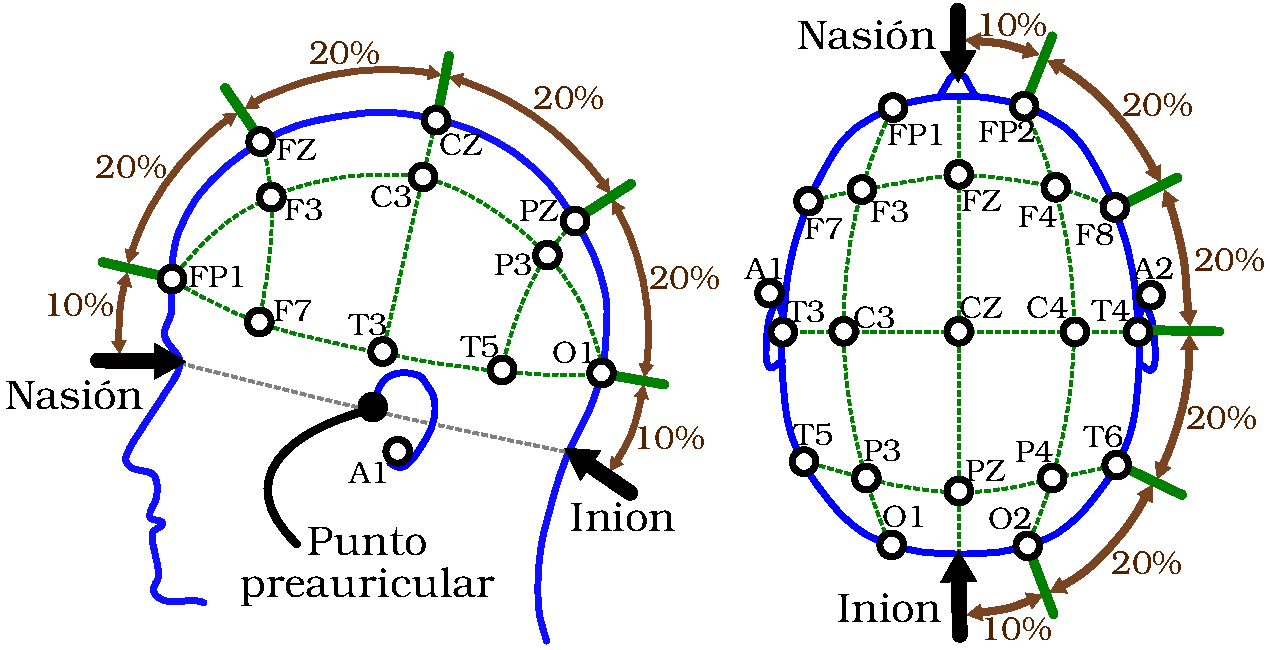
\includegraphics[width=0.9\linewidth]{./img_diagramas/cabeza_hecha.pdf} 
\caption{Colocaci\'on de electrodos seg\'un el sistema 10--20. En el cr\'aneo, el \textbf{inion} es 
una protuberancia craneal, mientras que el \textbf{nasi\'on} es la uni\'on del hueso frontal y los 
huesos nasales; el \textbf{punto preauricular} se ubica arriba del cart\'ilago llamado tragus, que 
protege el canal auditivo \cite{Butkov07}. 
}
\label{img1020}
\end{figure}

Usualmente el EEG muestra una actividad oscilatoria continua y cambiante, cuya 
frecuencia var\'ia entre 0.5 y 100 Hz \cite{Clark98}.
Su composici\'on est\'a fuertemente relacionada con el grado de actividad 
cerebral; por ejemplo, hay diferencias claras durante vigilia y sue\~no.
En general la frecuencia del EEG incrementa cuando hay un altos grados de actividad cerebral, lo 
cual se debe a que las ondas se vuelven m\'as as\'incronas, y entonces la magnitud del  potencial 
integrado de superficie decrece (a pesar de la alta actividad cortical).
Aunque la mayor parte del tiempo el EEG es irregular y no muestra patrones claros, es com\'un que 
muestre ondas cerebrales relativamente organizadas llamadas \textbf{ondas cerebrales} que, 
para su estudio, han sido clasificadas en 
cuatro grandes grupos: alfa, beta, gamma, delta.
Estos grupos son ilustrados en la figura \ref{ritmos}.

\begin{figure}
\centering
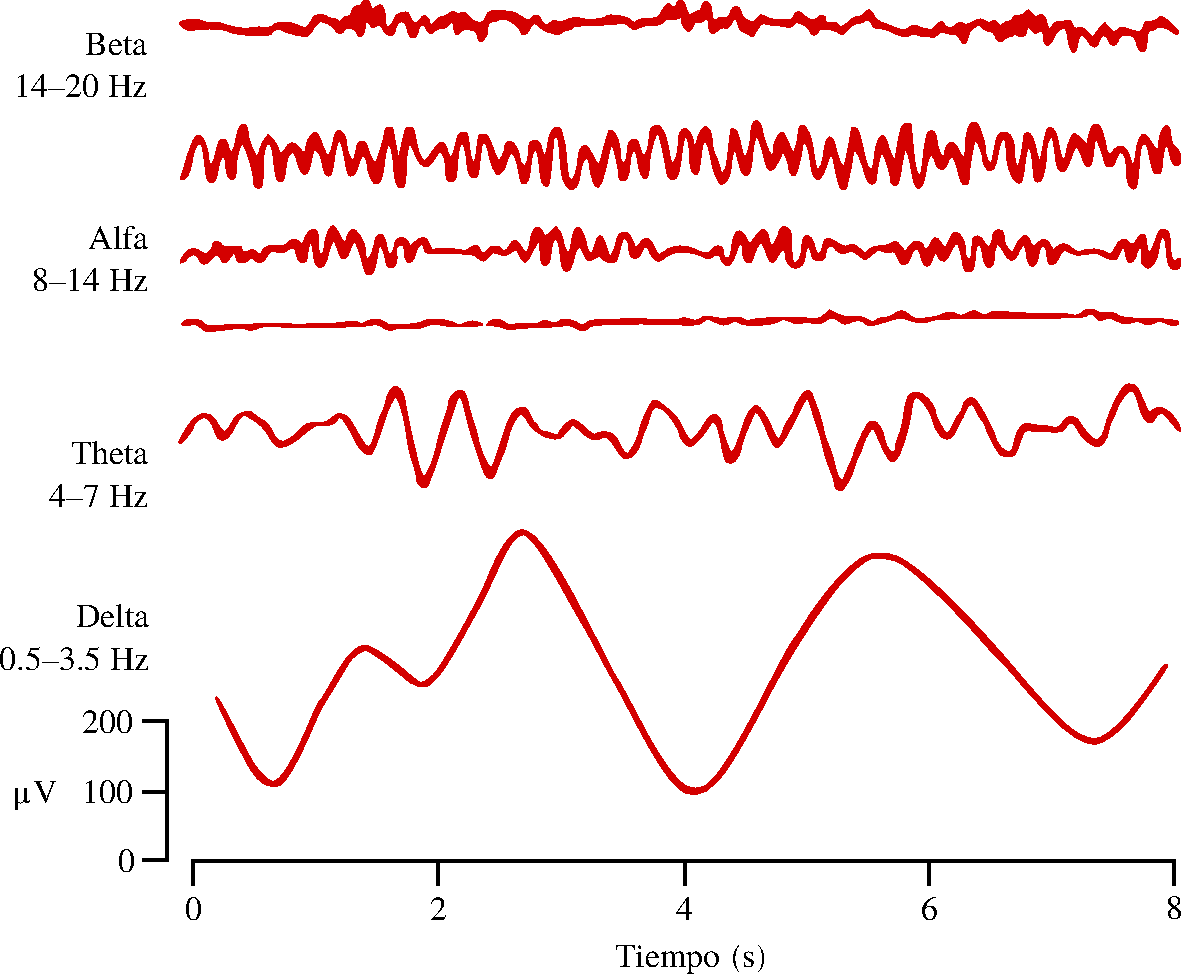
\includegraphics[width=0.55\linewidth]{./img_diagramas/ritmos_hechos.pdf} 
\caption{Ejemplos de ondas cerebrales encontradas en el EEG. Reconstruido de \textit{EEG Signal 
Processing}, por S. Sanei y J. A. Chambers \cite{Sanei07} }
\label{ritmos}
\end{figure}

\begin{description}
\item[Ondas alfa.] Frecuencias entre 8 y 13 Hz. Ocurren en sujetos despiertos en un estado de 
quietud del pensamiento. 
Aparecen m\'as frecuentemente en la regi\'on occipital, pero tambi\'en 
pueden ser registradas en las regiones frontal y parietal. 
%Su voltaje aproximado est\'a entre 20 y 
%200 mV. Cuando el sujeto duerme, las ondas alfa desaparecen completamente. 

\item[Ondas beta.] Frecuencias de 14 a 30 Hz. Normalmente se registran en las regiones parietal y 
frontal. 
%A veces se les divide en dos tipos: beta I y beta II. Las ondas beta I (14--20 Hz) son 
%afectadas por la actividad mental de manera similar a las ondas alfa.
%Las ondas beta II (20--30 Hz), en cambio, aparecen durante una activaci\'on intensa del sistema 
%nervioso central y durante tensi\'on.

\item[Ondas theta.] Frecuencias entre 4 y 7 Hz. Ocurren principalmente en las regiones parietal y 
temporal 
%en ni\~nos, pero pueden aparecer en algunos adultos durante estr\'es emocional, sobre todo 
%durante periodos de decepci\'on y frustraci\'on.

\item[Ondas delta.] Incluye todas las ondas del EEG con frecuencias menores a 3.5 Hz. Ocurren 
generalmente en el sue\~no profundo en infantes, y despu\'es de enfermedades org\'anicas serias del 
cerebro.
\end{description}

Cabe mencionar que el espectro de frecuencias del potencial de campo producido por m\'usculos 
faciales medianamente contra\'idos incluye componentes de frecuencia que bien cuadran en el rango 
usual del EEG (0.5--100 Hz); cuando estas se\~nales 'contaminan' el registro de EEG, son referidas
como \textbf{artefactos}. La variedad de artefactos conocidos es muy basta, al grado de
considerarse a la detecci\'on de \'estos como un paso previo inevitable.

%%%%%%%%%%%%%%%%%%%%%%%%%%%%%%%%%%%%%%%%%%%%%%%%%%%%%%%%%%%%%%%%%%%%%%%%%%%%%%%%%%%%%%%%%%%%%%%%%%%
%%%%%%%%%%%%%%%%%%%%%%%%%%%%%%%%%%%%%%%%%%%%%%%%%%%%%%%%%%%%%%%%%%%%%%%%%%%%%%%%%%%%%%%%%%%%%%%%%%%

\subsection{Sue\~no}

El sueño del ser humano, según criterios polisomnográficos (electroencefalograma, electrooculograma y electromiograma) se divide fundamentalmente en sueño REM (R) (rapid eye movement) y en sueño No REM (NREM)

El sue\~no normal se divide en dos etapas principales: MOR (fase R) y NMOR (fase N), que se 
diferencian por sus rasgos electroencefalogr\'aficos y una serie de caracter\'isticas 
fisiol\'ogicas, y de los cuales obtienen sus nombres.
Cabe mencionar que la nomenclatura acerca de las fases del sue\~no ha sido recientemente modificada 
por la American Association of Sleep Medicine (AASM) en 2007 \cite{AASM07}, de modo que en este 
trabajo se  usar\'an ambas nomenclaturas siempre que sea posible, por fines de compatibilidad.

\begin{description}
\item[Sue\~no] Proceso vital c\'iclico complejo y activo, compuesto por varias fases y que posee 
una estructura interna caracter\'istica, con diversas interrelaciones en los sistemas hormonales y 
nerviosos \cite{FernandezConde07}.
El sue\~no en el ser humano se puede caracterizar por las siguientes 
propiedades\cite{CarrilloMora}:
\begin{enumerate}
\item Disminuci\'on de conciencia y reactividad a est\'imulos externos
\item F\'acilmente reversible (lo cual lo diferencia de otros estados 
patol\'ogicos como el estupor y el coma)
\item Inmovilidad y relajaci\'on muscular
\item Periodicidad t\'ipica circadiana (diaria)
\item Los individuos adquieren una postura estereotipada
\item La privaci\'on induce alteraciones conductuales y 
fisiol\'ogicas, adem\'as de que genera una 'deuda' acumulativa
\end{enumerate}
\end{description}

Durante el sue\~no MOR (fase R), ocurre que las ondas lentas y amplitud alta son reemplazadas por 
ondas r\'apidas de bajo voltaje, irregulares, y que recuerdan la actividad en el EEG durante el 
estado de alerta.
La presencia de estos patrones irregulares no interrumpen el sue\~no, sino que incrementan el 
umbral para los est\'imulos externos; este comportamiento es referido como 'sue\~no parad\'ojico'.
Durante esta etapa de sue\~no, el sujeto exhibe movimientos oculares r\'apidos (MOR), raz\'on por 
la cual recibe su nombre caracter\'istico.
Durante el sue\~no MOR se producen la mayor\'ia de las enso\~naciones (referidos coloquialmente 
como sue\~nos), y la mayor\'ia de los pacientes que despiertan durante esta fase suelen recordar 
v\'ividamente el contenido de sus enso\~naciones \cite{Chokroverty09}.
F\'isicamente el tono de todos los m\'usculos disminuye (con excepci\'on de los m\'usculos 
respiratorios y los esf\'interes vesical y anal), as\'i mismo la frecuencia cardiaca y respiratoria 
se vuelve irregular.

El sue\~no fuera de la etapa MOR es referido como no-MOR (NMOR, fase N), y es dividido en etapas 
seg\'un la 'profundidad' del sue\~no, entendida en t\'erminos de la actividad cerebral registrada.
En el sue\~no profundo se observan ondas delta muy irregulares, y junto con ellas ocurren trenes 
cortos de ondas, parecidas a las alfa, y que son referidas como \textit{husos de sue\~no}. 
El ritmo alfa y los husos de sue\~no est\'an sincronizados en el sue\~no y la somnolencia, en 
contraste con la actividad irregular, desincronizada y de bajo voltaje registrada en estado de 
alerta.
A grosso modo, la clasificaci\'on de etapas del sue\~no seg\'un la AASM se basa en las siguientes
caracter\'isticas \cite{Hori01}:

\begin{description}
\item[Vigilia (W)] Presencia de ritmo alfa contin\'uo con m\'axima amplitud sobre regiones de la 
corteza parieto-occipital. Tono muscular relativamente alto y ausencia de movimientos oculares.

\item[Fase 1 (N1)] Corresponde con la somnolencia o el inicio del sue\~no ligero, en ella es muy 
f\'acil despertarse. 
Presencia intermitente de ondas alfa en menos del 50\% de la \'epoca, actividad de frecuencias 
mezcladas y bajo voltaje, adem\'as de movimientos oculares lentos y algunas ondas agudas. 
La actividad muscular disminuye paulatinamente, pueden observarse sacudidas musculares s\'ubitas 
que a veces coinciden con una sensaci\'on de ca\'ida. 

\item[Fase 2 (N2)] Se caracteriza por patrones espec\'ificos de actividad cerebral conocidos como 
husos de sue\~no y complejos K. 
Puede aparecer hasta un 20\% de ondas lentas (ritmo delta). Ausencia de actividad ocular y tono 
muscular bajo.
La temperatura, la frecuencia card\'iaca y respiratoria disminuyen paulatinamente. 

\item[Fases 3 (N3)] Predominan ondas de frecuencias muy bajas ($<2$ Hz) con amplitudes superiores a 
75 $\mu$V en m\'as del 20\% y menos del 50\% de la \'epoca. Pueden tambi\'en aparecer complejos K y 
husos de sue\~no de forma espor\'adica. Ausencia de actividad ocular y tono muscular bajo.

\item[Fase 4 (N4)] La fase m\'as profunda del sue\~no NMOR y referido como 'sue\~no de ondas 
lentas', pues hay presencia de \'estas ondas en m\'as del 50\% de la \'epoca. Las dem\'as 
caracter\'isticas son similares a las de la fase 3.

\item[Fase MOR (R)] Presencia de actividad EEG de baja amplitud y frecuencias entremezcladas 
(theta-alfa-beta) similar a la observada en el estado de vigilia activa con ojos abiertos.
\end{description}

Un adulto joven pasa aproximadamente entre 70--100 minutos en el sue\~no NMOR para despu\'es entrar 
al sue\~no MOR, el cual puede durar entre 5--30 min; este ciclo se repite cada hora y media.
En los ancianos se va fragmentando el sue\~no nocturno con frecuentes episodios de despertar, se 
reduce mucho el porcentaje de sue\~no en fase 4, pero se mantiene constante el porcentaje de 
sue\~no MOR. Adicionalmente, muchos adultos mayores dormitan durante el d\'ia varias siestas cortas 
\cite{CarrilloMora}.

La edad es un factor decisivo para la cantidad de horas de sueño. El recién nacido duerme entre 14 y 18 horas, el lactante entre 12 y 14 horas, el niño en etapa escolar entre 11 y 12 horas y en la edad adulta, la mayoría duerme entre 7 y 8 horas por noche. En otras palabras, es fisiológico que el número de horas dormidas vaya disminuyendo progresivamente a lo largo de la vida, pudiendo existir una diferencia de hasta 16 horas como promedio entre la niñez y la edad adulta. En los ancianos, el número de horas de diferencia entre las horas de sueño propias v/s las horas de sueño de la niñez, es aún mayor

\cite{Contreras13}

%%%%%%%%%%%%%%%%%%%%%%%%%%%%%%%%%%%%%%%%%%%%%%%%%%%%%%%%%%%%%%%%%%%%%%%%%%%%%%%%%%%%%%%%%%%%%%%%%%%
%%%%%%%%%%%%%%%%%%%%%%%%%%%%%%%%%%%%%%%%%%%%%%%%%%%%%%%%%%%%%%%%%%%%%%%%%%%%%%%%%%%%%%%%%%%%%%%%%%%
%%%%%%%%%%%%%%%%%%%%%%%%%%%%%%%%%%%%%%%%%%%%%%%%%%%%%%%%%%%%%%%%%%%%%%%%%%%%%%%%%%%%%%%%%%%%%%%%%%%
%%%%%%%%%%%%%%%%%%%%%%%%%%%%%%%%%%%%%%%%%%%%%%%%%%%%%%%%%%%%%%%%%%%%%%%%%%%%%%%%%%%%%%%%%%%%%%%%%%%

%%%%%%%%%%%%%%%%%%%%%%%%%%%%%%%%%%%%%%%%%%%%%%%%%%%%%%%%%%%%%%%%%%%%%%%%%%%%%%%%%%%%%%%%%%%%%%%%%%%
%%%%%%%%%%%%%%%%%%%%%%%%%%%%%%%%%%%%%%%%%%%%%%%%%%%%%%%%%%%%%%%%%%%%%%%%%%%%%%%%%%%%%%%%%%%%%%%%%%%
%%%%%%%%%%%%%%%%%%%%%%%%%%%%%%%%%%%%%%%%%%%%%%%%%%%%%%%%%%%%%%%%%%%%%%%%%%%%%%%%%%%%%%%%%%%%%%%%%%%
%%%%%%%%%%%%%%%%%%%%%%%%%%%%%%%%%%%%%%%%%%%%%%%%%%%%%%%%%%%%%%%%%%%%%%%%%%%%%%%%%%%%%%%%%%%%%%%%%%%

\section{Conceptos}

Para poder identificar marcadores significativos para el diagnóstico del deterioro cognitivo, 
éste debe ser estudiado desde la neuropsicología; dentro de ésta última se destaca la técnica de 
electroencefalografía, que es usada para medir cierto tipo de actividad cerebral y que posiblemente 
esté asociada al deterioro cognitivo. 
Una vez expuestos los conceptos pertinentes, se presenta una colección de objetos matemáticos
(procesos estocásticos débilmente estacionarios) con los cuales se han modelado un tipo de
actividad cerebral, y que fue comparado con mediciones de la misma.

La exposición se divide en dos subsecciones marcadamente diferentes: matemáticas y 
fisiología/psicología.
En la primera se menciona al deterioro cognitivo en adultos mayores, con énfasis en su 
caracterización dentro del sistema nervioso.
La segunda subsección se centra en las herramientas estadísticas utilizadas para analizar datos 
experimentales, entendidas no como simples \textit{técnicas} sino como objetos abstractos
definidos formalmente.

Estas dos partes difieren no sólo en temas sino también epistemológicamente: en la
primera aparecen afirmaciones basadas en datos experimentales, acompañadas de las citas 
pertinentes, mientras que en la segunda las
afirmaciones son formalmente verdaderas y demostrables en el sistema 
axiomático usual. Respecto a estas últimas, varias de las demostraciones se presentan como 
apéndice junto las definiciones pertinentes, mientras otras son citadas debido a diversos motivos.

\subsection{Psicología}

%La demencia es un síndrome debido a la disfunción cerebral, que produce desintegración
%de la conducta en los planos intelectual y emocional, alterando significativamente la
%función social y laboral del paciente.

La \textbf{demencia} es, según el Manual diagnóstico de y estadístico de trastornos mentales
(DSM-IV), \textit{un síndrome que consiste en el desarrollo de déficit cognoscitivos
suficientemente graves como para interferir significativamente en las actividades laborales 
y sociales, respecto al nivel de actividad previo. 
%Aparece precedida por una enfermedad médica o
%el efecto de exposición prolongada a sustancias tóxicas, incluso ambos.
Los sujetos con demencia tienen una baja capacidad para aprender información nueva y 
suelen olvidar lo aprendido anteriormente, siendo éste el síntoma más prominente} \cite{DCM_5}.

Cuando un sujeto presenta cambios marcados en su conducta, es relativamente fácil identificar
la demencia; caso contrario es el diagnóstico temprano de la misma, el cual es importante
para un tratamiento adecuado que 
revierta o desacelere el avance de este síndrome.
Se ha señalado que los criterios del manual DSM-IV son suficientes para este diagnóstico
\cite{Knopman01}.


Considerando a los \textbf{adultos mayores}, entendidos como individuos de 60 años o más,
conviene destacar que el
envejecimiento es determinado por una serie de procesos moleculares, celulares, fisiológicos y 
psicológicos que conducen directamente al deterioro de funciones cognitivas, específicamente 
atención y memoria \cite{Navarrete03,Park09}.
%Aunque popularmente se asocia a la vejez con el deterioro cognitivo,
La funcionalidad durante esta etapa se relaciona con el estilo de vida, los factores de riesgo, el 
acceso a la educación y las acciones para el cuidado de la salud realizadas en edades más 
tempranas \cite{Ohayon04,Sanhueza14}.
%En un principio, se consideraba que el envejecimiento cerebral ocurr\'ia fundamentalmente por una 
%muerte neuronal \cite{Coleman87}, sin embargo, estudios realizados con tejido cerebral post mortem 
%de adultos mayores que en vida fueron sanos, mostraron que dicha muerte neuronal no alcanza un 10\% 
%del tejido \cite{Esiri07}. 

%Con el paso del tiempo, la organizaci\'on an\'atomo-funcional del cerebro sufre modificaciones que 
%traen como consecuencia la afectaci\'on de diferentes capacidades cognitivas; sin embargo, la 
%vulnerabilidad de los circuitos neuronales ante estos cambios no suceden de forma homog\'enea en 
%todo el cerebro \cite{Hita14}.

Al momento de diagnosticar deterioro cognitivo en adultos mayores, deben tenerse en cuenta
el envejecimiento normal y la posible \textbf{pseudodemencia depresiva}, ya que presentan
características similares. Con respecto a ésta última, definida como \textit{un
trastorno del afecto y que produce un aparente deterioro cognitivo} \cite{DCM_5},
aunque no es efectivamente un tipo de demencia bien puede desencadenar en ello
en ausencia de un tratamiento adecuado.

Como es usual, se considerará como etapa precursora de la demencia al
\textbf{deterioro cognitivo leve}, definido como \textit{un
síndrome caracterizado por una alteración adquirida y prolongada de una o varias funciones 
cognitivas, que no corresponde a un síndrome focal y no cumple criterios suficientes de 
gravedad para ser calificada como demencia} \cite{Robles02}.
En el transcurso de este escrito este padecimiento
será manejado como \textbf{posible deterioro cognitivo (PDC)} ya
que el autor no tiene la autoridad ni la autorización para efectuar un diagnóstico clínico, y 
porque los síntomas en esta etapa se consideran --afortunadamente-- reversibles.


\subsubsection{Diagnóstico de la demencia}

En psicología los instrumentos de medición estándar son las \textbf{pruebas neuropsicológicas}, 
entendidas como muestras
de alguna conducta de interés a las que se asignan puntajes para comparar cuantitativamente
entre sujetos \cite{Ardila12}.

Las habilidades medibles a través de test neuropsicológicas se suelen agrupar en áreas o
\textbf{dominios}: atención, lenguaje, cálculo, memoria y aprendizaje, percepción,
motricidad, funciones somatosensoriales, habilidades espaciales, funciones ejecutivas. 
%Principales sindromes neuropsicologicos
%Afasia 
%Alexia 
%Agrafia 
%Acalculia 
%Agnosia 
%Apraxia 
%Amnesia 
%Sindrome disejecutivo 
%Demencia
%No  existe  un  manual  de  síndromes  neuropsicológicos,  aunque  muchos  de  ellos  se incluyen 
%en el Manual Diagnóstico y Estadístico de los Trastornos Mentales (DSM-IV, 1994)  y  en  la 
%Clasificación  Internacional  de  las  Enfermedades (ICD-10,  World  Health Organization, 2007).

HACER, QUIZA, UN CUADRO SOBRE LOS DOMINIOS Y SUS RELACIONES CON LAS PARTES DEL CEREBRO

%%%%%%%%%%%%%%%%%%%%%%%%%%%%%%%%%%%%%%%%%%%%%%%%%%%%%%%%%%%%%%%%%%%%%%%%%%%%%%%%%%%%%%%%%%%%%%%%%%%
%%%%%%%%%%%%%%%%%%%%%%%%%%%%%%%%%%%%%%%%%%%%%%%%%%%%%%%%%%%%%%%%%%%%%%%%%%%%%%%%%%%%%%%%%%%%%%%%%%%

\subsection{Fisiología}

El sistema nervioso central consiste en la médula espinal y el cerebro, siendo el segundo una
porción altemente especializada del primero; aparece protegido por las meninges, un grpo de tres capas 
protectoras, e inmerso en el llamado líquido cefalorraquídeo.
El cerebro se divide en tres partes: tallo cerebral, cerebelo y hemisferios cerebrales;
éstos últimos tienen asociadas las llamadas \textit{funciones superiores}, como son uso de lenguaje,
reconocimiento de rostros, aprendizaje, conciencia, etc., por lo que se les prestará
atención de forma exclusiva.

Los hemisferios cerebrales se componen de capas, de las cuales la más externa se conoce como
\textit{corteza cerebral}; tiene cerca de 1 cm de espesor y un color grisáceo debido a que
las céulas nerviosas en esa capa están muy densamente emapquetadas, y debido a lo cual se le conoce
como \textit{materia gris}.

La corteza cerebral presenta numerosos pliegues organizados en \textit{giros} (crestas) y
\textit{surcos} (valles), los surcos más profundos se llaman \textit{fisuras} y son usados
como referencia;
la fisura lateral define al \textbf{lóbulo temporal} como la porción por debajo de 
éste, mientras que la fisura central define al \textbf{lóbulo frontal} como la
porción delante de éste (ver figura \ref{lobulos}). Los \textbf{lóbulos parietal y occipital}
se encuentran, respectivamente, detrás de los lóbulos frontal y temporal.

Varias de las funciones superiores han sido asociadas con 

\begin{figure}
\centering
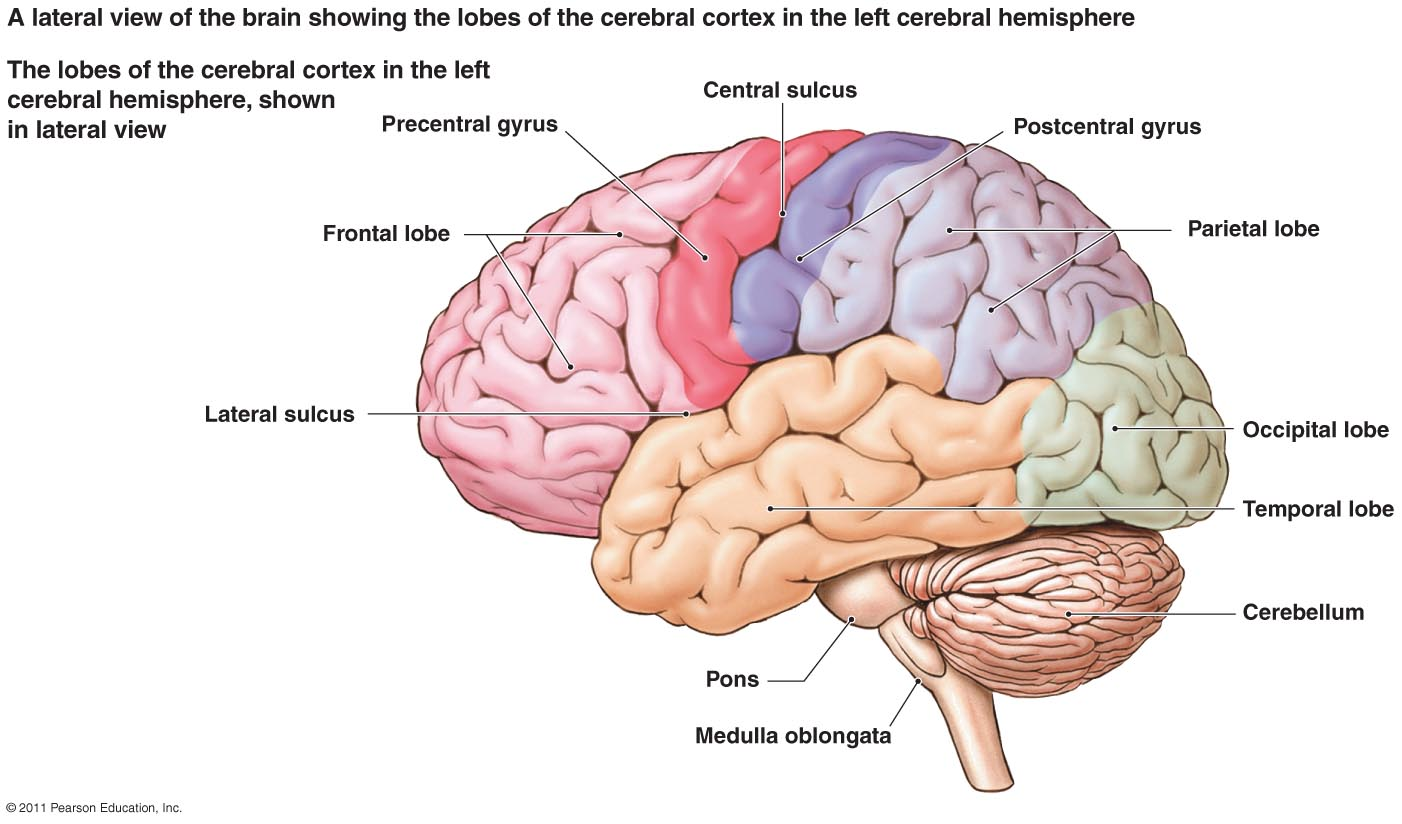
\includegraphics[width=0.8\linewidth]{./img_diagramas/brainlandmarks.jpg} 
\caption{Referentes fisiológicos usadas para definir a los lóbulos cerebrales.
Este gráfico será redibujado.
}
\label{lobulos}
\end{figure}

\begin{figure}
\centering
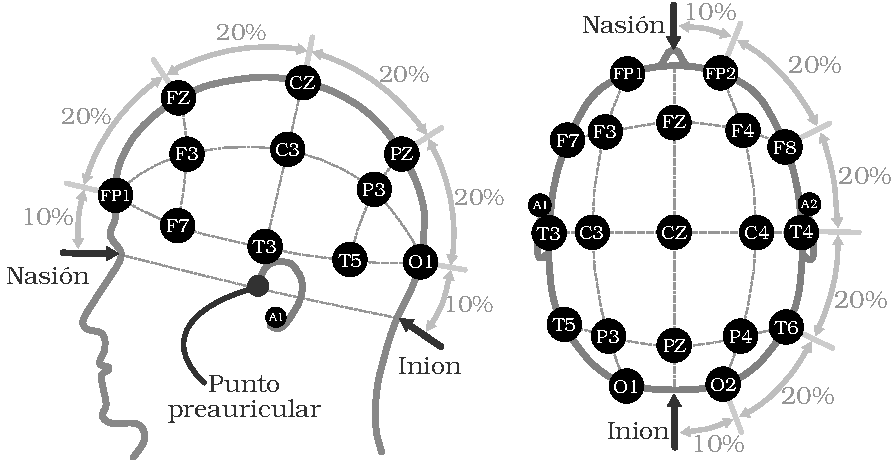
\includegraphics[width=\linewidth]{./img_diagramas/cabeza_proporcionada.pdf} 
\caption{Colocación de electrodos según el sistema 10--20. El \textbf{inion} es 
una protuberancia craneal, mientras que el \textbf{nasión} es la unión del hueso frontal y los 
huesos nasales; el \textbf{punto preauricular} se ubica arriba del cartílago llamado tragus, que 
protege el canal auditivo \cite{Butkov07}. 
}
\label{img1020}
\end{figure}

\begin{figure}
\centering
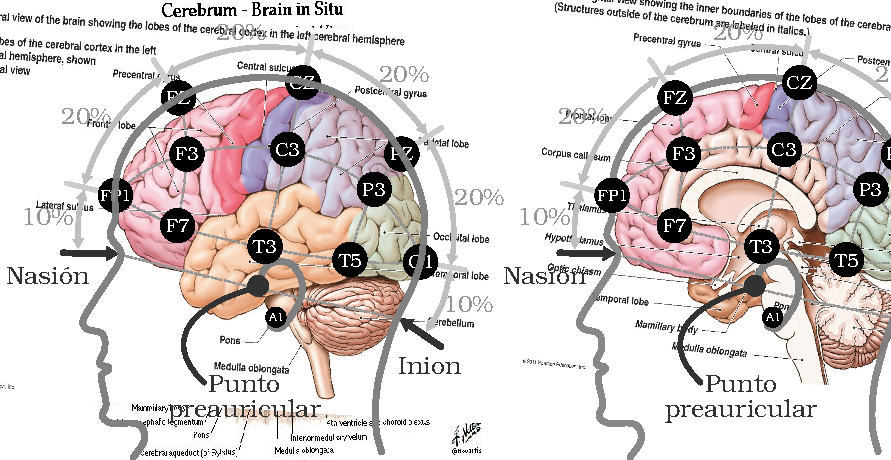
\includegraphics[width=\linewidth]{./img_diagramas/cerebro_1020.pdf} 
\caption{Esquema de la correspondencia entre el Sistema 10-20 y las regiones de la corteza
cerebral que representan, aproximadamente. Este gráfico será reconstruido.
}
\label{corresponde_1020}
\end{figure}

%%%%%%%%%%%%%%%%%%%%%%%%%%%%%%%%%%%%%%%%%%%%%%%%%%%%%%%%%%%%%%%%%%%%%%%%%%%%%%%%%%%%%%%%%%%%%%%%%%%
%%%%%%%%%%%%%%%%%%%%%%%%%%%%%%%%%%%%%%%%%%%%%%%%%%%%%%%%%%%%%%%%%%%%%%%%%%%%%%%%%%%%%%%%%%%%%%%%%%%

\subsection{Sueño}

%textwidth: \printinunitsof{cm}\prntlen{\textwidth}
%
%linewidth: \printinunitsof{cm}\prntlen{\linewidth}

%%%%%%%%%%%%%%%%%%%%%%%%%%%%%%%%%%%%%%%%%%%%%%%%%%%%%%%%%%%%%%%%%%%%%%%%%%%%%%%%%%%%%%%%%%%%%%%%%%%
%%%%%%%%%%%%%%%%%%%%%%%%%%%%%%%%%%%%%%%%%%%%%%%%%%%%%%%%%%%%%%%%%%%%%%%%%%%%%%%%%%%%%%%%%%%%%%%%%%%
%%%%%%%%%%%%%%%%%%%%%%%%%%%%%%%%%%%%%%%%%%%%%%%%%%%%%%%%%%%%%%%%%%%%%%%%%%%%%%%%%%%%%%%%%%%%%%%%%%%
%%%%%%%%%%%%%%%%%%%%%%%%%%%%%%%%%%%%%%%%%%%%%%%%%%%%%%%%%%%%%%%%%%%%%%%%%%%%%%%%%%%%%%%%%%%%%%%%%%%


%%%%%%%%%%%%%%%%%%%%%%%%%%%%%%%%%%%%%%%%%%%%%%%%%%%%%%%%%%%%%%%%%%%%%%%%%%%%%%%%%%%%%%%%%%%%%%%%%%%%
%%%%%%%%%%%%%%%%%%%%%%%%%%%%%%%%%%%%%%%%%%%%%%%%%%%%%%%%%%%%%%%%%%%%%%%%%%%%%%%%%%%%%%%%%%%%%%%%%%%
%%%%%%%%%%%%%%%%%%%%%%%%%%%%%%%%%%%%%%%%%%%%%%%%%%%%%%%%%%%%%%%%%%%%%%%%%%%%%%%%%%%%%%%%%%%%%%%%%%%
%%%%%%%%%%%%%%%%%%%%%%%%%%%%%%%%%%%%%%%%%%%%%%%%%%%%%%%%%%%%%%%%%%%%%%%%%%%%%%%%%%%%%%%%%%%%%%%%%%%

\section{Conceptos, matem\'aticas}

Se describen algunos conceptos sobre estimaci\'on espectral para procesos estoc\'asticos 
d\'ebilmente estacionarios (incluyendo las definiciones de \'estos), y la generalizaci\'on 
propuesta por Priestley para procesos no-estacionarios; esta descripci\'on se basa principalmente 
en libro \textit{Spectral Analysis and Time Series} de M. B. Priestley \cite{Priestley81}.

Como se mencion\'o, el objeto de estudio en este trabajo son registros de se\~nales
electrofisiol\'ogicas (en particular, de PSG) que son modeladas como procesos estoc\'asticos; (por 
simplicidad, se escribir\'a simplemente 'procesos'); antes de continuar, conviene presentar la 
definici\'on de este concepto. 

\begin{defn}[Proceso estoc\'astico]
Un proceso estoc\'astico $\{ X(t) \}$ es una familia de variables aleatorias en los reales, 
indexadas por $t \in T$.
\label{proc_estocastico}
\end{defn}

Se denotar\'a a una realizaci\'on de $X(t)$ como $x(t)$, mientras que la funci\'on de probabilidad 
acumulada para $X(t)$ ser\'a $F_{X(t)}$. Cabe enfatizar que para cada valor de $t$, $X(t)$ es una 
variable  aleatoria.

La definici\'on \ref{proc_estocastico} es aplicable tanto para procesos en tiempo continuo como 
para tiempo discreto\footnote{Un proceso se dice \textbf{a tiempo discreto} cuando el \'indice $t$ 
(tradicionalmente asociado al tiempo) pertenece a un conjunto a lo m\'as numerable, mientras que se 
dice \textbf{a tiempo continuo} si este conjunto es un intervalo; en este trabajo s\'olo se 
consideran estos dos tipos de 'tiempos'}.
Como modelo, se entiende que las se\~nales del PSG son fen\'omenos a tiempo continuo, pero que no
es registrable sino en un conjunto finito de puntos en el tiempo; en otras palabras, se espera que 
tenga caracter\'isticas propias de un proceso a tiempo continuo aunque en la pr\'actica se trate 
con un proceso a tiempo discreto.

\subsection{Estacionariedad d\'ebil}

Una vez definidos los procesos estoc\'asticos, es posible definir una caracter\'istica de los 
mismos y que se investiga en el presente trabajo: la estacionariedad.
Informalmente, esta propiedad se refiere a que la 'estructura' del proceso sea invariante en el
tiempo; para un proceso estacionario, calcular el promedio sobre cualquier subconjunto de datos 
deber\'ia arrojar resultados estad\'isticamente id\'enticos, mientras que no hay tal garant\'ia
para proceso no-estacionarios.
La definici\'on \ref{est_fuerte}, referida como estacionariedad fuerte o estricta, induce fielmente 
estas propiedades.

\begin{defn}[Estacionariedad fuerte]
Un proceso estoc\'astico $\{ X(t) \}$ es fuertemente estacionario si, para cualquier conjunto de 
tiempos admisibles\footnote{El t\'ermino \textbf{tiempos admisibles} indica que la definici\'on es 
la misma para procesos a tiempo discreto o continuo bajo las restricciones adecuadas} 
$t_1,t_2,\dots,t_n$ y cualquier $\tau$ tal que $t_i+\tau$ son tiempos admisibles para 
$i = 1, 2, \dots n$; se cumple que
\begin{equation*}
F_{\left(X(t_1),X(t_2),\dots,X(t_n)\right) }
\equiv
F_{\left(X(t_1+\tau),X(t_2+\tau),\dots,X(t_n+\tau)\right)}
\end{equation*}

Donde $F_{\left(X(t_1),X(t_2),\dots,X(t_n)\right) }$ es la funci\'on de distribuci\'on de 
probabilidad conjunta para el vector $\left(X(t_1),X(t_2),\dots,X(t_n)\right)$
\label{est_fuerte}
\end{defn}

Sin embargo, la definici\'on \ref{est_fuerte} resulta in\'util si se pretende verificar que un 
registro dado pudiera ser modelado como la realizaci\'on de un proceso es fuertemente estacionario 
(un objetivo descartado para este trabajo). En ese escenario, para cada tiempo registrado $t$ se 
tiene s\'olo una observaci\'on para cada variable aleatoria $X(t)$, lo cual es muy poca 
informaci\'on como para estimar las funciones de probabilidad acumulada mencionadas en la 
definici\'on.
Estas limitaciones motivan una definici\'on m\'as d\'ebil de estacionariedad, pero que pueda ser 
detectada en realizaciones dadas de procesos; se exhibe la definici\'on \ref{est_orden_m} como 
alternativa.

\begin{defn}[Estacionariedad de orden $\boldsymbol{m}$]
Un proceso estoc\'astico $\{ X(t) \}$ se dice estacionario de orden $m$ si, para cualquier conjunto 
de tiempos admisibles $t_1,t_2,\dots,t_n$ y cualquier $\tau \in \R$ se cumple que
\begin{equation*}
\E{ X^{m_1}(t_1)X^{m_2}(t_2)\cdots X^{m_n}(t_n) }
=
\E{ X^{m_1}(t_1+\tau)X^{m_2}(t_2+\tau)\cdots X^{m_n}(t_n+\tau) }
\end{equation*}
Para cualesquiera enteros $m_1,m_2,\dots,m_n$ tales que $m_1+m_2+\dots+m_n \leq m$
\label{est_orden_m}
\end{defn}

Para entender mejor la definici\'on \ref{est_orden_m} y sus limitaciones frente a la 
estacionariedad fuerte, consid\'erense tres procesos: $\{X(t)\}$ fuertemente estacionario, 
$\{Y_1(t)\}$ estacionario de orden 1, y $\{Y_2(t)\}$ estacionario de orden 2. Luego
\begin{itemize}
\item Las medias\footnote{La media de una variable aleatoria $V$ se define como $ \mu_V := \E{V}$} 
$ \mu_{X(t)}$, $ \mu_{Y_1(t)}$ y $ \mu_{Y_2(t)}$ no dependen de $t$

\item Las varianzas\footnote{La varianza de una variable aleatoria $V$ se define como 
$ \Var{V} := \E{\left(V - \mu_V \right)^{2}}$} $ \Var{Y_1(t)}$ y $ \Var{Y_2(t)}$ no dependen de 
$t$, pero no se puede garantizar lo mismo para $\Var{X(t)}$

\item El coeficiente de asimetr\'ia\footnote{El coeficiente de asimetr\'ia para una variable 
aleatoria $V$ se define como 
$\gamma_V = \frac{\E{\left(V-\mu_V\right)^{3}}}{\Var{V}^{\nicefrac{3}{2}}}$}
$ \gamma_{X(t)}$ no depende de $t$, pero no se puede garantizar lo mismo para $ \gamma_{Y_1(t)}$ ni 
para $ \gamma_{Y_2(t)}$
\end{itemize}

Cabe mencionar que hay una relaci\'on de contenci\'on clara en familia de los conjuntos de procesos 
estacionarios de orden finito (si un proceso es estacionario de orden $m$, entonces es estacionario 
de orden $n$ para todo $n \leq m$); es posible definir procesos estacionarios de orden 'infinito' 
seg\'un \ref{est_orden_m}, que intuitivamente ser\'ian fuertemente estacionarios. 
De manera pragm\'atica, en este trabajo no se discuten tales interrogantes, sino que se usar\'a 
\'unicamente la definici\'on correspondiente al caso $m=2$, referida como estacionariedad d\'ebil o 
de orden 2, y repetida en la definici\'on \ref{est_orden_2}.

\begin{defn}[Estacionariedad d\'ebil]
Un proceso estoc\'astico $\{ X(t) \}$ es d\'ebilmente estacionario si, para cualesquiera tiempos 
admisibles $t, s, t+\tau, s+\tau$, se cumple que
\begin{center}
\begin{tabular}{ccc}
$\E{X(t)} = \E{X(t+\tau)}$
& y &
$\E{X(t)X(s)} = \E{X(t+\tau)X(s+\tau)}$
\end{tabular}
\end{center}
\label{est_orden_2}
\end{defn}

M\'as a\'un, parece conveniente exhibir una caracterizaci\'on equivalente para los procesos 
d\'ebilmente estacionarios, pero que tiene una interpretaci\'on m\'as sencilla.
\begin{thrm}
Un proceso estoc\'astico es d\'ebilmente estacionario si y s\'olo si para cualesquiera tiempos 
admisibles $t$, $s$ se tiene que
\begin{itemize}
\item $\E{X(t)} = \mu_X$
\item $\Var{X(t)} = \sigma^{2}_X$
\item $\Cov{X(t),X(s)} = \rho_X (s-t)$
\end{itemize}
Donde $\mu_X$, $\sigma^{2}_X$ son constantes, $\rho_X(\tau)$ es una funci\'on que \'unicamente 
depende de $\tau$
\label{est_usual}
\end{thrm}

Cabe comentar  sobre la existencia de procesos que son fuertemente estacionarios pero que no son 
estacionarios de ning\'un orden: por ejemplo, un proceso de variables aleatorias independientes con 
distribuci\'on de Cauchy\footnote{Una variable aleatoria tiene distribuci\'on de Cauchy si su 
funci\'on de probabilidad acumulada es de la forma 
$\displaystyle F(x) = \frac{1}{\pi} \int_{-\infty}^{x} \frac{1}{1+y^{2}} dy$}.
Una condici\'on suficiente para que un proceso fuertemente estacionario sea estacionario de orden 
$m$ es que tenga sus primeros $m$ momentos bien definidos.
Con respecto a las se\~nales registradas en el EEG, entendidas como procesos estoc\'asticos, se 
espera que tengan (cuando menos) segundos momentos bien definidos; m\'as adelante se presentan 
argumentos, desde una interpretaci\'on f\'isica, sobre por qu\'e se espera que ocurra lo anterior.

A continuaci\'on (definici\'on \ref{cont_est}) se presenta una tipo de regularidad que se supone
para las se\~nales registradas en el EEG: continuidad de alg\'un tipo.

\begin{defn}[Continuidad estoc\'astica en media cuadr\'atica]
Un proceso estoc\'astico a tiempo continuo $\{ X(t) \}$ es estoc\'asticamente continuo, en el 
sentido de media cuadr\'atica, en un tiempo admisible $t_0$ si y s\'olo si
\begin{equation*}
\lim_{t \rightarrow t_0} \E{\left( X(t) - X(t_0) \right)^{2}} = 0
\end{equation*}
\label{cont_est}
\end{defn}

Una forma natural de pensar en la definici\'on \ref{cont_est} es que, si $\abso{t-t_0}$ es muy 
peque\~no, entonces $X(t)$ y $X(t_0)$ difieren muy poco entre s\'i (como variables aleatorias).
Es destacable que si un proceso es estoc\'asticamente continuo en un intervalo, sus realizaciones 
solamente se pueden garantizar continuas casi en todas partes \footnote{Una propiedad se cumple 
\textbf{casi en todas partes} si se cumple en un conjunto cuyo complemento tiene medida cero} en 
ese intervalo.
Como ejemplos, un proceso ruido blanco (definici\'on \ref{r_blanco}) no es estoc\'asticamente 
continuo, mientras que un proceso de Wiener (definici\'on \ref{r_wiener}) s\'i lo es.

\begin{defn}[Proceso ruido blanco]
Se dice de un proceso estoc\'astico $\{ R(t) \}$ que cumple, para cualesquiera tiempos admisibles
$t$ y $s$, las siguientes propiedades:
\begin{itemize}
\item $\E{R(t)}=0$
\item $\Cov{R(t),R(s)}=0 \Leftrightarrow t=s$ 
\end{itemize}
\label{r_blanco}
\end{defn}

\begin{defn}[Proceso de Wiener]
Se dice de un proceso estoc\'astico $\{ W(t) \}$ que cumple, para cualesquiera tiempos admisibles
$t$ y $s$ (con $s>t$) las siguientes propiedades:
\begin{itemize}
\item $W(0) = 0$ ($W(0)$ es constante)
\item $W(s)-W(t)$ es independiente de $W(u)$, para todo $u<t$ admisible
\item $W(s)-W(t) \sim N(0,\abso{t-s})$  (los incrementos tienen distribuci\'on normal)
\end{itemize}
\label{r_wiener}
\end{defn}

%%%%%%%%%%%%%%%%%%%%%%%%%%%%%%%%%%%%%%%%%%%%%%%%%%%%%%%%%%%%%%%%%%%%%%%%%%%%%%%%%%%%%%%%%%%%%%%%%%%
%%%%%%%%%%%%%%%%%%%%%%%%%%%%%%%%%%%%%%%%%%%%%%%%%%%%%%%%%%%%%%%%%%%%%%%%%%%%%%%%%%%%%%%%%%%%%%%%%%%

\subsection{Espectro de potencias para procesos estoc\'asticos}

Existe una larga tradici\'on en ciencias biom\'edicas para entender/modelar las se\~nales
electrofisiol\'ogicos en t\'erminos de ondas y frecuencias, ya que fundamentalmente son fen\'omenos 
el\'ectricos \cite{Kaiser00}.  
Estos modelos est\'an t\'ipicamente asociados con las series de Fourier y la transformada de 
Fourier (definiciones \ref{FourierClasico} y \ref{trFourier}, respectivamente).

\begin{defn}[Serie de Fourier]
Sea $k$ una funci\'on real peri\'odica (con periodo $2T$) tal que 
$\simint{T} \abso{k(t)} dt < \infty$. 
Se le llamar\'a 'serie de Fourier para la funci\'on $k$' a la sucesi\'on $\left( A_n \right)$, 
calculada de la siguiente manera
\begin{equation*}
A_n = \frac{1}{2 T} \simint{T} k(t) e^{-\nicefrac{ i n t}{2T}} dt
\end{equation*}
\label{FourierClasico}
\end{defn}

\begin{defn}[Transformada de Fourier]
Sea $P_T$ el espacio de las funciones peri\'odicas con periodo $2T$ que tienen una serie de Fourier 
bien definida. Existe una funci\'on $\mathfrak{F}$ que mapea cada funci\'on a su respectiva serie 
de Fourier, y \'esta ser\'a referida como la transformada de Fourier
\label{trFourier}
\end{defn}

Como se mencion\'o, en este trabajo se suponen conocidas las propiedades de las series de Fourier 
(seg\'un la definici\'on \ref{FourierClasico}), de entre las cuales se destacan las siguientes:
\begin{itemize}
\item Las series de Fourier  son cuadrado-sumables\footnote{Una sucesi\'on $\left( S_n \right)$ se 
dice cuadrado-integrable si cumple que $\sum_{n\in \mathbb{Z}} \abso{S_n}^{2} < \infty$. El 
conjunto de estas series es denotado por $\ell^{2}$}

\item La transformada de Fourier, $\mathfrak{F}$, no es invertible en general. Es com\'un definir
una pseudoinversa como 
$\mathfrak{F}_{\text{inv}} 
: \left( A_n \right) \mapsto \sum_{n \in \mathbb{Z}} A_n e^{\nicefrac{i n t}{2 T}} $

\item Los conjuntos $P_T$ y $\ell^{2}$, con la suma y producto usuales, tienen la estructura de 
espacio vectorial. M\'as a\'un, usando las respectivas normas $\Vert k \Vert = \intR k(t) dt$ y 
$\left\Vert \left( A_n \right) \right\Vert_2 = \sum_{n\in \mathbb{Z}} \abso{S_n}^{2} < \infty$,
ambos son espacios de Hilbert.
\end{itemize}

La transformada de Fourier goza de una interpretaci\'on f\'isica muy extendida, seg\'un la cual 
toda se\~nal peri\'odica puede verse como la superposici\'on (suma) de se\~nales senoidales 
ortogonales de diferentes frecuencias\footnote{De manera pragm\'atica, en el presente trabajo la 
palabra  'frecuencia' se usar\'a para referirse a la cantidad $q$ en expresiones del tipo 
$e^{i q t}$}; suponiendo previamente que las se\~nales se suman y multiplican por escalares de la 
manera usual. 
Esta afirmaci\'on es equivalente a que el conjunto de funciones con una serie de Fourier bien 
definida, tiene estructura de espacio vectorial y admite una base ortonormal de funciones 
senoidales (referida como la base de Fourier). 
La interpretaci\'on f\'isica adquiere mayor relevancia cuando se exhibe el concepto de energ\'ia
disipada (definici\'on \ref{energia}) en conjunto con el el teorema \ref{parseval_serie}, ya que 
permite formular la siguiente interpretaci\'on: la energ\'ia disipada por una se\~nal peri\'odica 
puede verse como la suma de la energ\'ia disipada por sus componentes en la base de Fourier 
(usualmente referidos como \textbf{componentes de frecuencias}).
La funci\'on que 'desglosa' estos componentes se conoce como espectro de potencias (definici\'on 
\ref{espec}).

\begin{defn}[Energ\'ia de una se\~nal]
Sea $k$ una funci\'on real que modela una se\~nal. La energ\'ia disipada por $k$ en el intervalo de
tiempo $[a,b]$ est\'a dada por
\begin{equation*}
\text{Energ\'ia}_{[a,b]} = \int_{a}^{b} \abso{k\left(t\right)}^{2} dt
\end{equation*}
\label{energia}
\end{defn}

\begin{thrm}[Relaci\'on de Parseval]
Sea $k$ una funci\'on peri\'odica (de periodo $2T$) que admite una serie de Fourier bien definida,
$(A_n)$. Se cumple que
\begin{equation*}
\int_T^{T} X^{2}(t) dt = \sum_{n=-\infty}^{\infty} \abso{A_n}^{2}
\end{equation*}
\label{parseval_serie}
\end{thrm}

\newpage

\begin{defn}[Espectro de potencias]
Sea $P_T$ el espacio de las funciones peri\'odicas con periodo $2T$ que tienen una serie de Fourier 
bien definida. Se le llama espectro de potencias a la funci\'on 
$h: P_T \times \mathbb{R} \mapsto \mathbb{R}$ definida como
\begin{equation*}
h_k(\omega) = 
\begin{cases}
\abso{A_i}^{2} & \text{ , si } \omega = \frac{n}{2T} \text{   con } n\in \mathbb{Z} \\
0 & \text{ ,  otro caso}
\end{cases}
\end{equation*}
donde $\left( A_n \right)$ es la serie de Fourier de $k$
\label{espec}
\end{defn}

Es importante mencionar que la energ\'ia, entendida como la integral de una forma cuadr\'atica, es 
un concepto com\'un a varias ramas de la f\'isica y las ingenier\'ias; en cambio, en econom\'ia o 
en epidemiolog\'ia, por ejemplo, no hay una motivaci\'on clara para usar el concepto de energ\'ia 
seg\'un \ref{energia}.
En el presente trabajo no s\'olo se manejar\'a este concepto de energ\'ia, sino que se supondr\'a
que los registros de PSG contienen energ\'ia finita para cualquier intervalo finito de tiempo.

%%%%%%%%%%%%%%%%%%%%%%%%%%%%%%%%%%%%%%%%%%%%%%%%%%%%%%%%%%%%%%%%%%%%%%%%%%%%%%%%%%%%%%%%%%%%%%%%%%%
%%%%%%%%%%%%%%%%%%%%%%%%%%%%%%%%%%%%%%%%%%%%%%%%%%%%%%%%%%%%%%%%%%%%%%%%%%%%%%%%%%%%%%%%%%%%%%%%%%%

\subsubsection{Espectro de potencias para funciones no-peri\'odicas}

A continuaci\'on se presentan dos generalizaciones de las series de Fourier previas, a aquella que
ser\'a usada para procesos estoc\'asticos. La primera de ellas es las integrales de Fourier
(definici\'on \ref{fourier_int}), que operan de la misma forma que las series de Fourier pero
sobre funciones absolutamente sumables; se pueden extender sencillamente la transformada de Fourier 
y el espectro de potencias para esta funci\'on.

\begin{defn}[Integral de Fourier]
Sea $k$ una funci\'on tal que $\intR \abso{k(t)} dt < \infty$. Se le llamar\'a 'integral de 
Fourier para la funci\'on $k$' a la funci\'on $A:\mathbb{R}\rightarrow \mathbb{C}$ calculada de la 
siguiente manera
\begin{equation*}
A(\omega) = \frac{1}{2 \pi} \intR k(t) e^{- i \omega t} dt
\end{equation*}
\label{fourier_int}
\end{defn}

La integral de Fourier  se encuentra bien definida para cualquier $\omega \in \mathbb{R}$, e 
incluso se puede probar que es una funci\'on continua y que converge a 0 en $\pm \infty$.
Sin embargo, por brevedad s\'olo se usar\'a como motivaci\'on para la transformada de 
Fourier-Stieltjes.

\begin{defn}[Transformada de Fourier-Stieltjes]
Se dice que una funci\'on real $A$ es la transformada de Fourier-Stieltjes de una funci\'on $k$ si 
\'esta puede expresarse casi en todas partes como
\begin{equation*}
k(x) = \intR e^{ i \omega t} dF(\omega)
\end{equation*}
siendo que la integral est\'a definida en el sentido de Stieltjes
\label{fourier_stieltjes}
\end{defn}

En la definici\'on \ref{fourier_stieltjes}, si $F$ es derivable en todas partes entonces $F\prima$ 
cumple el mismo papel que la integral de Fourier; en cambio, si $k$ es una funci\'on peri\'odica 
entonces $F$ toma una forma escalonada cuyos aumentos coinciden con la serie de Fourier para $k$. 
M\'as a\'un, existen funciones que no son ni peri\'odicas ni absolutamente sumables pero poseen 
una transformada de Fourier-Stieltjes, como $k(x)=\SEN{x}+\SEN{\sqrt{2}x}$, 
$k(x)=\COS{x} + (1+x^{2})^{-1}$.

\begin{comment}
\begin{thrm}[Descomposici\'on de Lebesgue]
Sea $f:I\rightarrow \R$ una funci\'on de variaci\'on acotada, con $I$ un intervalo. Entonces pueden 
hallarse funciones $f_j, f_c, f_a :I\rightarrow \R$ tales que
\begin{itemize}
\item $f = f_j+ f_c+ f_a$
\item $f_j = \sum_{y \leq x} f(x-0) + f(x+0)$
\item $f_a$ es absolutamente continua\footnote{Para que una funci\'on sea absolutamente continua,
basta que sea de variaci\'on acotada y que mapee conjuntos de medida cero en conjuntos de medida
cero} en $I$
\item $f_c$ es una funci\'on singular\footnote{Una funci\'on es singular si es continua, de 
variaci\'on acotada y no-constante, y se cumple que tiene derivada cero casi en todas partes} en 
$I$
\end{itemize}
Estas funciones son \'unicas excepto por constantes, y en conjunto son llamados la 
\textit{descomposici\'on de Lebesgue} de $f$
\label{Lebesgue_decomp}
\end{thrm}
\end{comment}

%%%%%%%%%%%%%%%%%%%%%%%%%%%%%%%%%%%%%%%%%%%%%%%%%%%%%%%%%%%%%%%%%%%%%%%%%%%%%%%%%%%%%%%%%%%%%%%%%%%
%%%%%%%%%%%%%%%%%%%%%%%%%%%%%%%%%%%%%%%%%%%%%%%%%%%%%%%%%%%%%%%%%%%%%%%%%%%%%%%%%%%%%%%%%%%%%%%%%%%

\subsubsection{Espectro de potencias para un proceso d\'ebilmente estacionario}

Por simplicidad, el enfoque la definici\'on que se aborda considera un proceso d\'ebilmente 
estacionario, $\{X(t)\}$, y posteriormente una realizaci\'on particular, $x(t)$; como no hay 
garant\'ia que $x$ tenga una transformada de Fourier bien definida (o alguna de las 
generalizaciones presentadas previamente), se procede a aproximarla por una serie de funciones que 
s\'i las tienen.
As\'i entonces, para cada $T>0$ se define a $x_T$ como
\begin{equation*}
x_T(t) = 
\begin{cases}
x(t) & \text{ , } -T\leq t \leq T \\
0 & \text{ , otro caso}
\end{cases}
\end{equation*}
Posteriormente se define a $G_T$; bien puede entenderse como una transformada de Fourier para una 
funci\'on extendida peri\'odicamente, y de modo que el espacio entre frecuencias se vuelven 
infinitesimal, o bien puede verse como una integral de Fourier (claramente bien definida) para una 
serie convergente de funciones.

\begin{equation*}
G_T (\omega) = \frac{1}{\sqrt{2 \pi}} \intR x_T(t) e^{-i \omega t} dt
= \frac{1}{\sqrt{2 \pi}} \int_{-T}^{T} x(t) e^{-i \omega t} dt
\end{equation*}

Sin la garant\'ia de que $x(t)$ tenga una integral de Fourier bien definida, no hay garant\'ia que 
$G_T$ converja cuando $T\rightarrow \infty$. Recuperando el concepto de energ\'ia disipada, ligado 
a $\left| G_T(\omega) \right|^{2}$, se puede construir una explicaci\'on f\'isica para la 
divergencia de $G_T$: un sistema que disipa 'niveles constantes' de energ\'ia (porque $\Var{X(t)}$ 
es constante) puede disipar una cantidad infinita de energ\'ia durante un tiempo infinito. 
Conviene, entonces, usar el tama\~no de los intervalos sobre los cuales se define $G_T$, de modo 
que se converja a una 'densidad' de energ\'ia disipada:
$\lim_{T\rightarrow{\infty}} \frac{ \left| G_T(\omega) \right|^{2}}{2 T}$.
Tal expresi\'on se puede adaptar al proceso per se como en la definici\'on \ref{SDF}.

\begin{defn}[Funci\'on de densidad espectral (SDF)]
Sea $\{X(t)\}$ un proceso estoc\'astico en tiempo continuo, d\'ebilmente estacionario. Se define la 
funci\'on de densidad espectral (SDF) para $\{X(t)\}$ como
%\begin{equation*}
%h(\omega) = \lim_{T\rightarrow \infty} \E{ \frac{ \left| G_T(\omega) \right|^{2}}{2 T} }
%\end{equation*}
\begin{equation*}
h(\omega) = \lim_{T\rightarrow \infty} \E{ \frac{1}{2T} \frac{1}{2 \pi}
\abso{ \int_{-T}^{T} X(t) e^{-i \omega t} dt}^{2} }
\end{equation*}
%Donde $G_T (\omega) = \frac{1}{\sqrt{2 \pi}} \int_{-T}^{T} X(t) e^{-i \omega t} dt$
\label{SDF}
\end{defn}

Conviene mencionar que la convergencia de la SDF est\'a garantizada casi en todas partes, pero la
funci\'on resultante puede no ser suficiente para explicar adecuadamente al proceso; por ejemplo, 
un proceso peri\'odico, con periodo $T$, tendr\'a una SDF que es cero en todos sus puntos salvo en 
los m\'ultiplos enteros de $T$.
Este fen\'omeno es similar al caso de variables aleatorias discretas, que no poseen una funci\'on 
de densidad de probabilidad bien definida en todos sus puntos.
Conviene definir una versi\'on 'integral' de la SDF (definici\'on\ref{SDF_integrado}).

\begin{defn}[Funci\'on de espectro integrado]
Sea $\{X(t)\}$ un proceso estoc\'astico a tiempo continuo, d\'ebilmente estacionario. Se define la 
funci\'on de espectro integrado para $\{X(t)\}$ como
\begin{equation*}
H(\omega) = \int_{-\infty}^{\omega} h(\lambda) d\lambda
\end{equation*}
Donde $h$ es la funci\'on de densidad espectral para $\{X(t)\}$
\label{SDF_integrado}
\end{defn}

Si la SDF, $h$, est\'a bien definida en todos sus puntos, entonces la funci\'on de espectro 
integrado ($H$) satisface que $H\prima= h$ y se dir\'a que el proceso tiene un \textbf{espectro 
puramente continuo}; si $H$ tiene una forma escalonada, con escalones rectos, se dir\'a que es un 
\textbf{espectro puramente discreto}.
Como es de esperarse, cada tipo de proceso tiene caracter\'istica diferentes y se puede estudiar 
mejor con herramientas diferentes; para el caso de procesos con un espectro mixto (ninguno de los 
anteriores), se exhiben herramientas que los reducen a estos casos 'puros'.

Cabe destacar que, por como se defini\'o la SDF integrada, \'esta es una funci\'on positiva, 
no-decreciente, y que en $-\infty$ vale 0; esta observaci\'on ser\'a importante.

%%%%%%%%%%%%%%%%%%%%%%%%%%%%%%%%%%%%%%%%%%%%%%%%%%%%%%%%%%%%%%%%%%%%%%%%%%%%%%%%%%%%%%%%%%%%%%%%%%%
%%%%%%%%%%%%%%%%%%%%%%%%%%%%%%%%%%%%%%%%%%%%%%%%%%%%%%%%%%%%%%%%%%%%%%%%%%%%%%%%%%%%%%%%%%%%%%%%%%%

\subsection{Estimaci\'on de la funci\'on de densidad espectral}

Anteriormente se defini\'o espectro de potencias para procesos d\'ebilmente estacionarios con 
segundos momentos finitos (definici\'on \ref{SDF}); sin embargo, aquella definici\'on es sumamente 
ineficiente dentro de la estimaci\'on pues requiere valores esperados sobre todo del proceso.
A continuaci\'on se muestran dos teoremas respecto a la SDF facilitar\'an su estimaci\'on.

\begin{thrm}[Wiener-Khinchin]
Una condici\'on suficiente y necesaria para que $\rho$ sea una funci\'on de autocorrelaci\'on de 
alg\'un proceso estoc\'astico a tiempo continuo $\{X(t)\}$ d\'ebilmente estacionario y 
estoc\'asticamente continuo, es que exista una funci\'on $F$ que tenga las siguientes propiedades
\begin{itemize}
\item Mon\'otonamente creciente
\item $F(-\infty) = 0$
\item $F(+\infty) = 1$
\end{itemize}
y tal que para todo $\tau \in \R$ se cumple que
\begin{equation*}
\rho(\tau) = \intR e^{i \omega \tau} dF(\omega)
\end{equation*}
\label{t_wienerkhinchin}
\end{thrm}

\begin{thrm}[Wold]
Una condici\'on suficiente y necesaria para que $\rho$ sea una funci\'on de autocorrelaci\'on de 
alg\'un proceso estoc\'astico a tiempo discreto $\{X(t)\}$ d\'ebilmente estacionario es que exista 
una funci\'on $F$ con las siguientes propiedades
\begin{itemize}
\item Mon\'otonamente creciente
\item $F(-\pi) = 0$
\item $F(+\pi) = 1$
\end{itemize}
y tal que para todo $\tau \in \R$ se cumple que
\begin{equation*}
\rho(\tau) = \intPI e^{i \omega \tau} dF(\omega)
\end{equation*}
\label{t_wold}
\end{thrm}

Una observaci\'on interesante sobre estos teoremas es el caso $\tau = 0$
\begin{equation*}
\rho(0) = \int_{-A}^{+A} dF(\omega) = F(A) - F(-A)
\end{equation*}
donde $A$ vale $\infty$ o $\pi$ seg\'un sea el caso discreto o continuo. Si $R$ es la funci\'on de
autocovarianza del proceso, entonces la ecuaci\'on anterior se traduce en que
\begin{equation*}
R(0) = \sigma^{2} \left( F(A) - F(-A) \right) = \sigma^{2} F(A)
\end{equation*}
donde $\sigma^{2}$ es la varianza del proceso. 
Esta observaci\'on adquiere importancia porque la SDF integrada ($H$), por definici\'on, satisface 
el papel de $F$ salvo por la condici\'on $F(\infty)=1$; si se puede garantizar que 
$H(\infty)<\infty$ entonces puede ser normalizada para satisfacer tal condici\'on y, m\'as a\'un,
si tal fuera el caso entonces $H(\infty)=\sigma^{2}$. Una consecuencia muy fuerte de este 
comentario es que, como se ha establecido previamente que s\'olo se considerar\'an procesos con
segundos momentos finitos, entonces la SDF de los procesos considerados siempre es acotada.

Como corolario, se puede afirmar que la SDF de un proceso (d\'ebilmente estacionario y de varianza
finita) es la transformada de Fourier-Stieltjes de la funci\'on de autocovarianza.
Esto implica que el estimador m\'as 'natural' para la SDF es la transformada de Fourier (discreta) 
de la funci\'on de autocorrelaci\'on (estimada); esta funci\'on se conoce como 
\textit{periodograma}. 

Conviene introducir estimadores para la funci\'on de autocovarianza de un proceso d\'ebilmente 
estacionario, $\{ X(t) \}$, a partir de un conjunto de $N$ observaciones equiespaciadas en el 
tiempo con separaci\'on $\Delta t$; se denotar\'a a estas observaciones como 
$x_1, x_2 , \dots, x_N$. Como se cumple la siguiente propiedad para la funci\'on de autocovarianza, 
$R$, por definici\'on
\begin{equation*}
R(\tau) = \E{X(n\Delta t)X(n\Delta t + \tau)} \text{  ,  } n = 0, 1, 2,  3,\dots, N
\end{equation*}
el estimados est\'andar para $R$ est\'a dado por la siguiente expresi\'on
\begin{equation*}
\widehat{R}(\tau) = \frac{1}{N-\abso{\tau}} 
\sum_{t = 1}^{N-\abso{\tau}} x_t x_{t+\abso{\tau}}
\label{estimador_R}
\end{equation*}

Se puede demostrar que $\widehat{R}$ es un estimador insesgado\footnote{Un estimador para el 
par\'ametro $\theta$, $\widehat{\theta}$, se dice \textbf{insesgado} si 
$\E{\widehat{\theta}}=\theta$} y consistente\footnote{Un estimador para el par\'ametro $\theta$ que 
depende de $N$ observaciones, 
$\widehat{\theta}_N$, se dice \textbf{consistente} si 
$\lim_{N\rightarrow \infty} \Var{\widehat{\theta}_N} = 0$} 
para $R$; sin embargo conviene introducir un estimador diferente para $R$
\begin{equation*}
\aste{R}(\tau) = \frac{1}{N} 
\sum_{t = 1}^{N-\abso{\tau}} x_t x_{t+\abso{\tau}}
\label{estimador_R_ast}
\end{equation*}

Se puede demostrar que $\aste{R}$ tiene las siguientes propiedades:
\begin{itemize}
\item $\E{\aste{R}(\tau)} = \left(1 - \frac{\abso{\tau}}{N} \right) R(\omega)$
\item $\Var{\aste{R}(\tau)} \approx \frac{1}{N} 
\sum_{r=-\infty}^{\infty} \left( R^{2}(r) + R(r-\tau)R(r+\tau) \right)$
\item $\Cov{\aste{\rho}(\tau),\aste{\rho}(\tau+\nu)} \approx \frac{1}{N} 
\sum_{r=-\infty}^{\infty} \left( \rho(r)\rho(r+\nu) + \rho(r-\tau)\rho(r+\tau+\nu) \right)$
\end{itemize}
Las aproximaciones para la varianza y covarianza se vuelven exactas si el proceso sigue una 
distribuci\'on normal en todos los tiempos.

Bajo estas consideraciones, se exhibe formalmente el periodograma (definici\'on 
\ref{periodograma}); si bien la expresi\'on con que se escribe es f\'acil de interpretar (la 
transformada de Fourier discreta para la se\~nal) y es eficiente computacionalmente, es conveniente
ligarla con la funci\'on de autocovarianza (teorema \ref{periodograma_rho}).

\begin{defn}[Periodograma]
Sean $x_1, x_2 , \dots, x_N$ observaciones de un proceso estoc\'astico de media cero y varianza
finita. Se llama periodograma a la funci\'on $I_N: [-\pi,\pi] \rightarrow \R$ calculada como
\begin{equation*}
I_N(\omega) = \frac{2}{N} \abso{ \sum_{t=0}^{N} e^{i \omega t} x_t }^{2}
\end{equation*}
\label{periodograma}
\end{defn}

\begin{thrm}
Sean $x_1, x_2 , \dots, x_N$ observaciones de un proceso estoc\'astico de media cero y varianza
finita. Se puede calcular el periodograma para estos datos como
\begin{equation*}
I_N(\omega) = 2 \sum_{r = -(N-1)}^{N-1} \aste{R}(r) \COS{r \omega}
\end{equation*}
Donde $\aste{R}$ es el estimador para la funci\'on de autocovarianza del proceso, calculado como
$\widehat{R}(\tau) = \frac{1}{N-\abso{\tau}} \sum_{t = 1}^{N-\abso{\tau}} x_t x_{t+\abso{\tau}}$
\label{periodograma_rho}
\end{thrm}

Se puede demostrar que el periodograma es un estimador insesgado de la SDF para los proceso 
considerados; sin embargo, si el proceso tuviera un espectro puramente continuo, ocurre que 
$\lim_{N\rightarrow \infty} \Var{I_N(\omega)} = h^{2}(\omega)$, con $h$ la SDF del proceso: el 
periodograma, en general, no es consistente.
En parte esto ocurre porque el periodograma depende de los estimadores para la funci\'on de 
autocovarianza, $\est{R}$, evaluada en todos los puntos posibles: para calcular $\est{R}$ en 
valores muy altos se requieren puntos muy alejados, los cuales son menos abundantes e implican 
una mayor varianza.

Si efectivamente el periodograma aumenta su varianza cuando incluye las 'colas' de la funci\'on de 
autocovarianza, entonces una soluci\'on es evitarlas, multiplicando por una funci\'on de pesos. 
Tales consideraciones dan origen a estimadores de la forma
\begin{equation*}
\est{h}(\omega) = \frac{1}{2\pi} \sum_{s = -(N-1)}^{N-1} 
\lambda(s) \aste{R}(s) e^{i \omega t}
\label{ventaneando}
\end{equation*}
donde la funci\'on de pesos, $\lambda$, es referida como \textbf{ventana de retrasos}. Para 
estudiar las propiedades estos estimadores, conviene reescribirlos en funci\'on del periodograma

\begin{equation*}
\est{h}(\omega) = \intPI I_N(\theta) W(\omega-\theta) d\theta
\end{equation*}
donde $W$ es la transformada de Fourier finita de $\lambda$
\begin{equation*}
W(\theta) = \frac{1}{2\pi} \sum_{s = -(N-1)}^{N-1} \lambda(s) e^{-is\theta}
\end{equation*}

Cabe destacar la forma que adopta $\est{h}$ como la convoluci\'on $I_N \ast W$, que bien puede 
entenderse como que $W$ es una funci\'on de pesos en el 'dominio de las frecuencias'; por ello, $W$ 
es referida como \textbf{ventana de retrasos}.
En la tabla \ref{ventanas} hay una lista corta de algunas funciones tipo ventana. Estos estimadores 
son consistentes y sesgados, aunque son asint\'oticamente insesgados.

\begin{SidewaysTable}
\centering
\bordes{1.5}
\begin{tabular}{c}
\textbf{Algunas funciones tipo ventana}
\vspace{1em}
\end{tabular}
\begin{tabular}{lll}
\toprule
 & \textbf{Ventana de retrasos} & \textbf{Ventana en las frecuencias} \\
\midrule
\textbf{P. truncado} & 
$\displaystyle
\lambda(s) = \begin{cases}
1 &\text{, si } \abso{s} \leq M \\
0 &\text{, otro caso}
\end{cases}$ &
$\displaystyle
W(\theta) = \frac{1}{2\pi} \frac{\SEN{(M+\frac{1}{2})\theta}}{\SEN{\nicefrac{\theta}{2}}}
=: D_M(\theta)$
\\
\rowcolor{gris}
\textbf{Bartlet} &
$\displaystyle
\lambda(s) = \begin{cases}
1-\nicefrac{\abso{s}}{M} &\text{, si } \abso{s} \leq M \\
0 &\text{, otro caso}
\end{cases}$ &
$\displaystyle
W(\theta) = \frac{1}{2\pi M} 
\left( \frac{\SEN{ \nicefrac{M\theta}{2}}}{\SEN{\nicefrac{\theta}{2}}} \right)^{2}
=: F_M(\theta)$
\\
\textbf{Daniell} &
$\displaystyle
\lambda(s) = \frac{\SEN{\nicefrac{\pi s}{M}}}{\nicefrac{\pi s}{M}}$ &
$\displaystyle
W(\theta) = \begin{cases}
\nicefrac{M}{2\pi} &\text{, si } \abso{\theta} \leq \nicefrac{\pi}{M} \\
0 &\text{, otro caso}
\end{cases}$
\\
\rowcolor{gris}
\textbf{Tukey-Hanning} &
$\displaystyle
\lambda(s) = \begin{cases}
\nicefrac{1}{2}\left( 1+ \COS{\nicefrac{\pi s}{M}} \right) &\text{, si } \abso{s} \leq M \\
0 &\text{, otro caso}
\end{cases}$ &
$\displaystyle
W(\theta) = \frac{1}{4} D_M\left(\theta - \frac{\pi}{M} \right) 
+\frac{1}{2} D_M\left(\theta \right)
\frac{1}{4} D_M\left(\theta + \frac{\pi}{M} \right)$
\\
\textbf{Parzen} &
$\displaystyle
\lambda(s) = \begin{cases}
1-6\left( \nicefrac{s}{M} \right)^{2} + 6\left( \nicefrac{\abso{s}}{M} \right)^{3} 
&\text{, si } \abso{s} \leq \nicefrac{M}{2} \\
2\left( 1 - \nicefrac{\abso{s}}{M} \right)^{3}
 &\text{, si } \nicefrac{M}{2} \leq \abso{s} \leq M \\
0 &\text{, otro caso}
\end{cases}$ &
$\displaystyle
W(\theta) = \frac{3}{8 \pi M^{3}} \left( 
\frac{\SEN{\nicefrac{M\theta}{4}}}{\nicefrac{1}{2}\SEN{\nicefrac{\theta}{2}}} 
\right)^{4}
\left( 1- \nicefrac{2}{3} \SEN{\nicefrac{\theta}{2}}^{2} \right)$
\\
\rowcolor{gris}
\textbf{Bartlet-Priestley} &
$\displaystyle
\lambda(s) = \frac{3M^{2}}{\left(\pi s\right)^{2} }
\left( \frac{\SEN{\nicefrac{\pi s}{M}}}{\nicefrac{\pi s}{M}} - \COS{\nicefrac{\pi s}{M}}
\right)
$ 
&
$\displaystyle
W(\theta) = \begin{cases}
\frac{3M}{4\pi} \left( 1- \left(\frac{M \theta}{\pi} \right)^{2} \right)
&\text{, si } \abso{\theta} \leq \nicefrac{\pi}{M} \\
0 &\text{, otro caso}
\end{cases}$
\\
\bottomrule
\end{tabular}
\caption{Ejemplos de algunas ventanas que suavizan el periodograma, formando estimadores 
consistente de la SDF para el caso de espectro puramente continuo.
Las funciones $F_M$ y $D_M$ toman, respectivamente, los nombres de \textit{n\'ucleo de Fejer} y
\textit{N\'ucleo de Dirichlet} de orden $M$}
\label{ventanas}
\end{SidewaysTable}

%%%%%%%%%%%%%%%%%%%%%%%%%%%%%%%%%%%%%%%%%%%%%%%%%%%%%%%%%%%%%%%%%%%%%%%%%%%%%%%%%%%%%%%%%%%%%%%%%%%
%%%%%%%%%%%%%%%%%%%%%%%%%%%%%%%%%%%%%%%%%%%%%%%%%%%%%%%%%%%%%%%%%%%%%%%%%%%%%%%%%%%%%%%%%%%%%%%%%%%

\subsection{Filtros lineales}

Como herramienta auxiliar en la estimaci\'on de la SDF, conviene considerar procesos del tipo 
$Y(t) = \intR g(u) X(t-u) du$, referidos como 'filtrados'.
Hist\'oricamente los filtros se originan como circuitos f\'isicos que, por dise\~no, son de ayuda 
en la 'cancelaci\'on' anal\'ogica de componentes de frecuencia (ver m\'as adelante).
%
Los filtros, aplicados a proceso d\'ebilmente estacionarios, afectan su SDF de manera 'simple' 
(teorema \ref{filtro}); por otro lado, permiten interpretar a procesos autorregresivos (AR) y de 
medias m\'oviles (MA) como versiones filtradas de procesos ruido blanco; m\'as a\'un, si los 
procesos filtrados pueden tener la forma\footnote{La integral est\'a definida en el sentido de 
Stieltjes} $Y(t) = \intR X(t-u) dG(u)$, entonces es posible manejar el operador retraso 
($B[Y](t) = Y(t)-Y(t-1)$).
%

\begin{thrm}
Sea $\{ X(t) \}$ un proceso d\'ebilmente estacionario que admite una representaci\'on de 
Wold-Cram\'er. Sea $g$ una funci\'on real con $\intR \abso{g(u)} du < \infty$, y sea $\{ Y(t) \}$ 
un proceso definido de la siguiente forma:
\begin{equation*}
Y(t) = \intR g(u) X(t-u) du
\end{equation*}
Entonces, se cumple la siguiente relaci\'on
\begin{equation*}
h_X(\omega) = h_Y(\omega) \abso{\Gamma(\omega)}^{2}
\end{equation*}
donde $h_X$ y $h_Y$ son las respectivas SDF de $\{X(t)\}$ y $\{Y(t)\}$, y 
$\Gamma(\omega) = \intR g(u) e^{i \omega u} du$.
\label{filtro}
\end{thrm}

En el teorema \ref{filtro}, la funci\'on $g$ es referida como \textbf{funci\'on de respuesta}; tal 
nombre tiene sentido si $\{X(t)\}$ no fuera un proceso, sino un 'impulso unitario' (una funci\'on 
tipo \dirac \footnote{La funci\'on $\delta_x:\R\rightarrow \R$ es una funci\'on $\delta$ de Dirac 
si puede verse como la funci\'on de distribuci\'on de masa para una medida finita que es cero para 
todo conjunto que no contenga a $x$}).
La funci\'on $\Gamma$ es referida como \textbf{funci\'on de transferencia}, nombre motivado de 
manera similar al considerar a $\{X(t)\}$ una 'se\~nal' senoidal ($X(t) = e^{i \omega t}$); la 
conexi\'on se vuelve m\'as clara si se interpreta esta segunda se\~nal como funci\'on tipo \dirac 
en el dominio de las frecuencias.
Respecto a la 'cancelaci\'on' de frecuencias basta decir que, en teor\'ia, se puede construir a $g$ 
de modo que $\Gamma$ sea 0 fuera de un intervalo cerrado y 1 dentro del mismo; este efecto es 
referido como \textbf{filtro de banda}.

%%%%%%%%%%%%%%%%%%%%%%%%%%%%%%%%%%%%%%%%%%%%%%%%%%%%%%%%%%%%%%%%%%%%%%%%%%%%%%%%%%%%%%%%%%%%%%%%%%%
%%%%%%%%%%%%%%%%%%%%%%%%%%%%%%%%%%%%%%%%%%%%%%%%%%%%%%%%%%%%%%%%%%%%%%%%%%%%%%%%%%%%%%%%%%%%%%%%%%%

\subsection{Representaci\'on de Wold-Cram\'er}

Como consecuencia de los teoremas \ref{t_wienerkhinchin} y \ref{t_wold}, los procesos d\'ebilmente 
estacionarios pueden ser caracterizados usando directamente la SDF (sin usar la funci\'on de
autocorrelaci\'on).
Esta representaci\'on existe en virtud del teorema \ref{rep_espectral}, cuya demostraci\'on no 
ser\'a incluida en este trabajo; el lector interesado en tan imponente teorema puede referirse a 
\cite{Priestley81}.

\newpage

\begin{thrm}
Sea $\{X(t)\}$ un proceso estoc\'astico a tiempo continuo d\'ebilmente estacionario de media 0 y 
estoc\'asticamente continuo en el sentido de media cuadr\'atica. Entonces, existe un proceso 
ortogonal $\{Z(\omega)\}$ tal que, para todo tiempo $\omega$ admisible, se puede 
escribir\footnote{La integral se encuentra definida en el sentido de media cuadr\'atica.}
\begin{equation*}
X(t) = \intR e^{i t \omega} dZ(\omega)
\end{equation*}
Donde el proceso $\{Z(t)\}$ tiene las siguientes propiedades para todo $\omega$
\begin{itemize}
\item $\E{dZ(\omega)} = 0$
\item $\E{\abso{dZ(\omega)}^{2}} = dH(\omega)$
\item $\Cov{dZ(\omega),dZ(\lambda)} = 0 \Leftrightarrow \omega \neq \lambda$
\end{itemize}
Donde $dH(\omega)$ la SDF integrada de $\{X(t)\}$
\label{rep_espectral}
\end{thrm}

En virtud del teorema de Wold, se puede tener una variante del teorema \ref{rep_espectral}
para procesos a tiempo discreto, raz\'on por la cual  
tal representaci\'on es referida como \textbf{representaci\'on de Wold-Cram\'er}.

%%%%%%%%%%%%%%%%%%%%%%%%%%%%%%%%%%%%%%%%%%%%%%%%%%%%%%%%%%%%%%%%%%%%%%%%%%%%%%%%%%%%%%%%%%%%%%%%%%%
%%%%%%%%%%%%%%%%%%%%%%%%%%%%%%%%%%%%%%%%%%%%%%%%%%%%%%%%%%%%%%%%%%%%%%%%%%%%%%%%%%%%%%%%%%%%%%%%%%%

\subsection{Prueba de Priestley-Subba Rao}

Esta t\'ecnica fue presentada por Priestley y Subba Rao en 1969 \cite{Priestley69}, y consiste en 
estimar el espectro local del proceso len varios puntos en el tiempo y las frecuencias, para luego 
probar la hip\'otesis de que el espectro cambia en el tiempo; la explicaci\'on presente es m\'as 
bien somera, los detalles formales que se omiten en el presente texto (la existencia del proceso 
evolutivo para cierto tipo de procesos, las propiedades de los estimadores usados) pueden 
encontrarse son tomadas de \cite{Priestley65} y \cite{Priestley66}.

Se pre-supone que los datos pueden entenderse como una cantidad finita de 
observaciones provenientes de un proceso estoc\'astico a tiempo continuo que, para todos los 
tiempos, tiene media cero y varianza finita, adem\'as de ser estoc\'asticamente continuo y tener 
un espectro puramente continuo.
Si bien son numerosas las condiciones, no se ha supuesto que
el proceso sea estacionario; adem\'as, se ha argumentado porqu\'e los que conviene ver a los 
registros de PSG  como observaciones de procesos, estoc\'asticamente continuos, con valor 
esperado y varianzas finitas. El tener media cero y espectro puramente continuo ser\'an 'forzadas' 
num\'ericamente, estimando del proceso su media y componente peri\'odica mediante regresi\'on
lineal adaptativa; en particular, se utiliza el algoritmo \textit{Seasonal-Trend decomposition
using Loess} (STL), propuesto por Cleveland y colaboradores \cite{Cleveland1990}.

Por brevedad, se mostrar\'a s\'olo someramente una condici\'on extra para los procesos a considerar:
tener una representaci\'on de la forma
\begin{equation*}
X(t) = \intPI A(t,\omega) e^{i t \omega} dZ(\omega)
\end{equation*}
donde $\{ dZ(\omega) \}$ es un proceso ortogonal 
($\Cov{dZ(\omega),dZ(\lambda)} = 0 \Leftrightarrow \omega \neq \lambda$).
Este objeto, que bien puede entenderse como una representaci\'on de Wold-Cram\'er que puede cambiar
en el tiempo, fue introducida por Priestley \cite{Priestley65} como el
\textbf{espectro evolutivo}; es amplia e interesante
la discusi\'on sobre qu\'e procesos admiten un espectro evolutivo, pero se omite en
el presente trabajo por motivos de tiempo.

Respecto a la estimaci\'on del espectro local se usa el \textbf{estimador de doble ventana}, 
t\'ecnica introducida por Priestley \cite{Priestley69} y que requiere dos funciones, $w_\tau$ y 
$g$, que funcionan como ventana de retrasos y como filtro lineal, respectivamente.
%
En cuando a $g$, se define a $\Gamma(u) = \intR g(u) e^{i u \omega} du$ y se les pide que
\begin{equation*}
2\pi \int_{-\infty}^{\infty} \lvert g(u) \lvert^{2} du 
= 
\int_{-\infty}^{\infty} \lvert \Gamma(\omega) \lvert^{2} d\omega
= 1
\end{equation*}

Cabe mencionar que las ventanas espectrales mostradas en la tabla \ref{ventanas} bien 
pueden cumplir las propiedades requeridas para ser filtros.
Posteriormente se define el estimador $U$ con el objetivo de asignar pesos en el tiempo para estimar
a la SDF
% en el tiempo dado; m\'as a\'un, $U$ sirve 
%como una aproximaci\'on de la representaci\'on de Wold-Cram\'er para 
%el proceso.
\begin{equation*}
U(t,\omega) = \int_{t-T}^{t} g(u) X({t-u}) e^{i \omega (t-u)} du
\end{equation*}

Bajo el entendido que la funci\'on $\Gamma$ converge a una funci\'on tipo \dirac, puede 
considerarse que 
$\E{\abso{U(t,\omega)}^{2}} \approx f_t(\omega)$; sin embargo, se demuestra en \cite{Priestley66} 
que $\Var{\abso{U(t,\omega)}^{2}} \nrightarrow 0$.
%
Debido a ello se usa una segunda funci\'on tipo ventana,
%, para 'suavizar' el estimador y hacerlo consistente (
de forma similar al periodograma.
Se considera la funci\'on $W_\tau$, ventana de retrasos, y su respectiva ventana espectral 
$w_\tau$; deben satisfacer las siguientes propiedades:
\begin{itemize}
\item $w_{\tau}(t) \geq 0$ para cualesquiera $t$, $\tau$
\item $w_{\tau}(t) \rightarrow 0$ cuando $\lvert t \lvert \rightarrow \infty$, para todo $\tau$
\item $\displaystyle \int_{-\infty}^{\infty} w_{\tau}(t) dt = 1$ para todo $\tau$
\item $\displaystyle \int_{-\infty}^{\infty} \left( w_{\tau}(t) \right)^{2} dt < \infty$ para todo $\tau$
\item $\exists C$ tal que  
$\displaystyle \lim_{\tau\rightarrow\infty} \tau \int_{-\infty}^{t} \abso{ W_{\tau}(\lambda) }^{2} d\lambda = C$
\end{itemize}

%Por ejemplo, la ventana de Daniell satisface estas propiedades; para ello, conviene calcular que
%$\lim_{\tau\rightarrow\infty} \tau \int_{t-T}^{t} \lvert W_{\tau}(\lambda) \lvert^{2} d\lambda = 2\pi$;
%m\'as a\'un, 
Cabe mencionar que todas las ventanas mostradas en \ref{ventanas} satisfacen las propiedades 
anteriores.
Finalmente, se define el estimador $\est{f}$ para las SDF normalizada, $f_t$, como
\begin{equation*}
\widehat{f}(t,\omega) = \int_{t-T}^{t} w_{T'}(u) \lvert U(t-u,\omega) \lvert^{2} du
\label{estimador_doble_ventana}
\end{equation*}

Fue demostrado por Priestley \cite{Priestley65} que los estimadores de doble ventana son 
asint\'oticamente insesgados y consistentes, y propone las siguientes aproximaciones:
%conviene exhibir las siguientes expresiones aproximadas propuestas en aqu\'el trabajo
\begin{itemize}
\item $\displaystyle
\E{\est{f}(t,\omega)} \approx 
\intR \widetilde{f}(t,\omega+\theta) \abso{\Gamma(\theta)}^{2} d\theta$
\item $\displaystyle
\Var{\est{f}(t,\omega)} \approx \frac{C}{\tau} \left( \overline{f}^{2}(\omega) \right)
\intR \abso{\Gamma(\theta)}^{4} d\theta $
\end{itemize}

donde las funciones $\widetilde{f}$ y $\overline{f}$ son versiones 'suavizadas' de la SDF 
normalizada, $f$, y est\'an definidas de la siguiente manera
\begin{equation*}
\widetilde{f}(t,\omega+\theta) = 
\intR W_{\tau}(u) f(t-u,\omega+\theta) du
\end{equation*}
\begin{equation*}
\overline{f}^{2} (t,\omega) =
\frac{\intR f^{2}\left(t-u,W_{\tau}^{2}(u)\right) du}
{\intR \left( W_{\tau}(u) \right)^{2} du}
\end{equation*}

Como $W_{\tau}$ funciona como ventana espectral, converge a una 
funci\'on tipo \dirac; luego $\widetilde{f}$ es aproximadamente la convoluci\'on 
$\widetilde{f}(t,\omega+\theta) \approx \delta_t \ast f(\bullet,\omega+\theta)$. 
Una aproximaci\'on muy similar 
puede hacerse respecto al segundo t\'ermino, de modo que $\widetilde{f}\approx f$ y 
$\overline{f}^{2}\approx f^{2}$.
Tales aproximaciones ser\'an mejores en tanto las ventanas $w_{\tau}$ y $W_{\tau}$ sean m\'as 
cercanas a funciones tipo \dirac.
%; m\'as a\'un, una condici\'on adecuada es que estas funciones 
%tengan una forma 'm\'as delgada' que el espacio entre los tiempos y frecuencias donde se estimar\'a 
%$f$.
Dicho esto, se pueden hacer las siguientes aproximaciones, un poco m\'as arriesgadas:
\begin{itemize}
\item $\displaystyle \E{\est{f}(t,\omega)} \approx f(t,\omega)$
\item $\displaystyle \Var{\est{f}(t,\omega)} \approx 
\frac{C}{\tau} f^{2}(t,\omega) \intR \abso{\Gamma (\theta)}^{4} d\theta$
\end{itemize}

%Por otro lado, es importante mostrar expresiones para la covarianza, si bien s\'olo se
%se reescriben 
%aqu\'i unas simplificaciones hechas en el caso que el proceso, adem\'as de cumplir las hip\'otesis 
%de semi-estacionariedad, sea 'normal'
A continuaci\'on se exhiben expresiones para la covarianza del estimador, en el caso particular
de un proceso aproximadamente normal
\begin{equation*}
\Cov{\est{f}(t_1,\omega_1) , \est{f}(t_2,\omega_2)} \approx \intR \intR
w_\tau (u) w_\tau(v) \Cov{ \abso{U(t_1-u,\omega_1)}^{2} , \abso{U(t_2-u,\omega_2)}^{2} }
du dv
\end{equation*}
la covarianza ser\'a negligible en tanto $w_\tau$ se comporte como una 
funci\'on \dirac, con un pico m\'as delgado que $\abso{\omega_1-\omega_2}$.
El mismo efecto se logra si $\abso{U(t_1-u,\omega_1)}^{2}$ y $\abso{U(t_2-u,\omega_2)}^{2}$ son 
no-correlacionados, pero por brevedad s\'olo se citar\'a de \cite{Priestley65} que basta que 
$\Gamma$ sea una funci\'on \dirac, cuyo ancho sea menor a $\abso{t_1-t_2}$.

Un dato sumamente importante para la estimaci\'on de la SDF es c\'omo la varianza del estimador 
$\widehat{f}$ depende 'multiplicativamente' de la verdadera SDF.
Una interpretaci\'on sobre este hecho, difundida dentro de las ingenier\'ias, es sobre la 
'modulaci\'on' de ondas, que puede verse como una 'multiplicaci\'on de ondas', y que motiva el uso 
de la 'transformaci\'on logar\'itmica'.
Formalmente, se introduce el siguiente estimador
\begin{equation*}
Y(t,\omega) = \log{\left( \est{f}(t,\omega)\right)}
\end{equation*}

Se puede demostrar que $Y$ tiene las siguientes propiedades:
\begin{itemize}
\item $\displaystyle 
\E{ Y(t,\omega) } \approx \log \left( f(t,\omega) \right)$
\item $\displaystyle 
\Var{ Y(T,\omega) } 
\approx \frac{C}{\tau} \intR \abso{\Gamma (\theta)}^{4} d\theta $
\end{itemize}
m\'as a\'un, el estimador $Y$ puede ser representado de la siguiente forma
\begin{equation*}
Y(t,\omega) = \log \left( f(t,\omega) \right) + \varepsilon(t,\omega)
\end{equation*}
donde las variables $\varepsilon(t,\omega)$ satisfacen que
\begin{itemize}
\item $\displaystyle \E{\varepsilon(t,\omega)} = 0$
\item $\displaystyle \Var{\varepsilon(t,\omega)}
\approx \frac{C}{\tau} \intR \abso{\Gamma (\theta)}^{4} d\theta$
\end{itemize}

Priestley \cite{Priestley81} destaca que la transformaci\'on logar\'itmica tiene la propiedad de 
hacer que el estimador $Y$ tenga una distribuci\'on 'm\'as cercana' a la normal, y que en la 
pr\'actica bien puede considerarse que las variables $\varepsilon$'s tienen distribuci\'on normal 
con media 0 y varianza $\sigma^{2}$.
Es destacable que las variables $\varepsilon$'s comparten la misma media y varianza, adem\'as de 
que son aproximadamente no-correlacionadas.

La prueba de Priestley-Subba Rao, como se mencion\'o, funciona calculando el estad\'istico $Y$ 
sobre varios puntos en el tiempo y la frecuencia, y luego revisando si se puede afirmar que el 
vector  $\left( Y(t,\omega_1), Y(t,\omega_2), \dots, Y(t,\omega_N) \right)$ es constante en el 
tiempo; de forma concreta  se maneja la siguiente aproximaci\'on
\begin{equation*}
\sum_{i = 1 }^{N} \left( Y(t,\omega_i) - \overline{Y}(\bullet,\omega_i) \right)^{2} 
\sim \sigma^{2} \chi^{2}(N)
\end{equation*}
donde $\sigma^{2} = \Var{\varepsilon(t,\omega)}$, y
$\overline{Y}(\bullet,\omega) = \frac{1}{M} \sum_{j=1}^{M} Y(t_j,\omega)$.
Con tal caracterizaci\'on se puede usar una prueba ANOVA de manera relativamente f\'acil.

%%%%%%%%%%%%%%%%%%%%%%%%%%%%%%%%%%%%%%%%%%%%%%%%%%%%%%%%%%%%%%%%%%%%%%%%%%%%%%%%%%%%%%%%%%%%%%%%%%%
%%%%%%%%%%%%%%%%%%%%%%%%%%%%%%%%%%%%%%%%%%%%%%%%%%%%%%%%%%%%%%%%%%%%%%%%%%%%%%%%%%%%%%%%%%%%%%%%%%%
%%%%%%%%%%%%%%%%%%%%%%%%%%%%%%%%%%%%%%%%%%%%%%%%%%%%%%%%%%%%%%%%%%%%%%%%%%%%%%%%%%%%%%%%%%%%%%%%%%%
%%%%%%%%%%%%%%%%%%%%%%%%%%%%%%%%%%%%%%%%%%%%%%%%%%%%%%%%%%%%%%%%%%%%%%%%%%%%%%%%%%%%%%%%%%%%%%%%%%%

%%%%%%%%%%%%%%%%%%%%%%%%%%%%%%%%%%%%%%%%%%%%%%%%%%%%%%%%%%%%%%%%%%%%%%%%%%%%%%%%%%%%%%%%%%%%%%%%%%%
%%%%%%%%%%%%%%%%%%%%%%%%%%%%%%%%%%%%%%%%%%%%%%%%%%%%%%%%%%%%%%%%%%%%%%%%%%%%%%%%%%%%%%%%%%%%%%%%%%%
%%%%%%%%%%%%%%%%%%%%%%%%%%%%%%%%%%%%%%%%%%%%%%%%%%%%%%%%%%%%%%%%%%%%%%%%%%%%%%%%%%%%%%%%%%%%%%%%%%%
%%%%%%%%%%%%%%%%%%%%%%%%%%%%%%%%%%%%%%%%%%%%%%%%%%%%%%%%%%%%%%%%%%%%%%%%%%%%%%%%%%%%%%%%%%%%%%%%%%%

\section{Matemáticas}

Existe una larga tradición para entender --y modelar-- las señales electrofisiológicas en términos 
de ondas y frecuencias, ya que fundamentalmente son fenómenos eléctricos \cite{Kaiser00}.
En el presente trabajo se aborda el enfoque usual de asociar la \textit{energía} de una señal con 
su varianza, y usar la transformada de Fourier para estudiar como se \textit{reparte} dicha energía
entre los \textit{componentes de frecuencia}. 
%
Para modelar los registros de PSG como procesos estocásticos conviene mencionar que
\begin{itemize}
\item Usar un modelo estocástico para las señales no implica suponer que son aleatorias, sino que 
en principio no se rechaza el no-determinismo
\item Las señales ocurren efectivamente \textit{a tiempo continuo} aunque sólo son 
registrables \textit{a tiempo discreto}, lo cual es importante dentro del modelo
\end{itemize}

El objetivo principal de este trabajo es estudiar si el modelo descrito admite --en el sentido 
estadístico-- algunas propiedades, entre las cuales destaca la estacionariedad débil, y cómo la 
información recabada durante la comparación puede relacionarse con las fases de sueño y el PDC.

%%%%%%%%%%%%%%%%%%%%%%%%%%%%%%%%%%%%%%%%%%%%%%%%%%%%%%%%%%%%%%%%%%%%%%%%%%%%%%%%%%%%%%%%%%%%%%%%%%%

\subsection{Frecuencia y energía}

%Para estudiar formalmente a la transformada de Fourier y sus propiedades, cuando menos las 
%relevantes como modelo, han de presentarse los espacios de funciones para las cuales \textit{tiene 
%sentido}; tarea que es ejecutada en el anexo A.

La \textbf{transformada de Fourier \textit{clásica}} ($\mathscr{F} $) se entiende formalmente como 
un operador\footnote{Un operador es efectivamente una función, cuyo dominio es un conjunto de 
funciones; toma un nombre distinto para evitar confusiones} que asocia una función $S=S(t)$,
periódica con periodo $2T$, con una serie $A = A(n),  {n\in \Z}$ tal que
\begin{equation}
A(n) = \frac{1}{2T} \int_{-T}^{T} S(t) e^{ -i t \frac{n}{2T}} dt
\label{txt_s_fourier}
\end{equation}
%
donde el factor $\frac{n}{2T}$ es referido como \textit{frecuencia}; y se dice que 
$\mathscr{F}[S] = A$. Los detalles formales sobre $\mathscr{F}$ se exponen en el anexo A.
%
Con respecto a la \textbf{energía}, de manera operativa ésta se define 
como\footnote{Potencia = Energía / Tiempo, ver anexo A}
\begin{equation}
\text{potencia}[S]_{[a,b]} = \frac{1}{b-a} \int_a^{b} \abso{S(t)}^{2} dt
\label{txt_potencia}
\end{equation}

La relación de Parseval permite caracterizar la potencia de una señal si ésta admite una tr. de
Fourier bien definida
%
\begin{equation}
\int_{-T}^{T} \abso{S(t)}^{2} dt = \sum_{n=-\infty}^{\infty} \abso{A(n)}^{2}
\label{txt_parseval}
\end{equation}

Reemplazando la expresión \ref{txt_parseval} sobre la definición de potencia, el módulo de la tr. 
de Fourier puede verse como indicador de como se \textit{distribuye} la energía de la señal $S$,
motivo por el cual es referido como \textbf{espectro de potencia}.
En las diferentes genralizaciones que se presentan, se busca conservar tal interpretación.
%
%Por ejemplo, si $S$ no es periódica pero cumple que $\intR \abso{S(t)} dt < \infty$, entonces
%puede definirse
%
%\begin{equation*}
%A(\omega) = \intR S(t) e^{- i \omega t} dt
%\end{equation*}


%%%%%%%%%%%%%%%%%%%%%%%%%%%%%%%%%%%%%%%%%%%%%%%%%%%%%%%%%%%%%%%%%%%%%%%%%%%%%%%%%%%%%%%%%%%%%%%%%%%

\subsection{Estacionariedad débil}

En el sentido formal un \textbf{proceso estocástico}\footnote{Durante el texto será referido 
simplemente como \textbf{proceso}, por comodidad} \xt es una colección de \textit{variables 
aleatorias} (VA) indexadas.
El significado preciso y formal de los conceptos mencionados en la presente sección se discuten en
el anexo B.

El conjunto $T \in \R$ que indexa a un proceso, referido como \textit{tiempo}, se considerará como 
un intervalo cerrado (\textbf{tiempo continuo}) o bien un suconjunto de 
$\left\{ t \in \R | {t} \cdot {\Delta_t} \in \Z \right\} $  para algún $\Delta_t$ 
(\textbf{tiempo discreto}).
Estos procesos suelen ser referidos como \textit{univariados} o \textit{series de tiempo}.
%
Las diferentes partes de un proceso estocástico serán denotadas como:\\

\begin{tabular}{cl}
\xt & Todo el proceso \\
$X(t)$ & Una VA que compone al proceso, en el tiempo $t$ \\
$x(t)$ & Una realización de $X(t)$ \\
$F_{X(t)}$ & Función de propbabilidad acumulada para $X(t)$ \\
$ {\Delta_t}$ & Frecuencia de muestreo (sólo en tiempo discreto)
\end{tabular}\\

La estacionariedad es un indicativo de la \textit{homogeneidad} de un proceso, un proceso 
fuertemente estacionario se compone de VA que tienen la misma distribución y distribuciones
conjuntas que no dependen del tiempo (definición ??); tal característica usualmente se considera
\textit{innecesariamente} fuerte y se reemplaza por la siguiente

\begin{definicion}%[Estacionariedad débil]
Un proceso \xt es \textbf{débilmente estacionario} si y sólo si para cualesquiera tiempos 
admisibles\footnote{\textbf{Tiempos admisibles} significa que la definición es la misma para tiempo
y discreto, bajo las restricciones pertinente} $t$, $s$ se tiene que
\begin{itemize}
\item $\E{X(t)} = \mu_X$
\item $\Var{X(t)} = \sigma^{2}_X$
\item $\Cov{X(t),X(s)} = R_X (s-t)$
\end{itemize}
Donde $\mu_X$, $\sigma^{2}_X$ son constantes, $\rho_X(\tau)$ es una función que únicamente 
depende de $\tau$
%\label{est_orden_primera}
\end{definicion}

Por simplicidad de notación, a lo largo del texto los procesos débilmente estacionarios serán 
referidos simplemente como \textit{estacionarios}. 

%%%%%%%%%%%%%%%%%%%%%%%%%%%%%%%%%%%%%%%%%%%%%%%%%%%%%%%%%%%%%%%%%%%%%%%%%%%%%%%%%%%%%%%%%%%%%%%%%%%

\subsection{Función de densidad espectral}

La forma más natural de definir un espectro de potencias para un proceso estacionario 
es a través de la tr. de Fourier de sus realizaciones; sin embargo, en general no se puede 
garantizar que quede bien definida: puede no ser periódica, cuadrado-integrable, uniformemente 
continua, etc.
%
Este problema se aborda restringiendo el tiempo a un conjunto \textit{sin problemas}, para luego
considerar el límite cuando tal conjunto tiende a su \textit{forma original}.

\begin{definicion}%[Función de densidad espectral]
Sea \xt un proceso estacionario a tiempo continuo. Se define su \textbf{función de densidad 
espectral} como
\begin{equation}
h(\omega) = \frac{1}{2 \pi} \lim_{T\rightarrow \infty} \E{ \frac{1}{2T} 
\abso{ \int_{-T}^{T} X(t) e^{-i \omega t} dt}^{2} }
\label{txt_FDE_cont}
\end{equation}
\end{definicion}

\begin{definicion}%[Función de densidad espectral]
Sea $\{X(t)\}_{\nicefrac{t}{\Delta_t}\in \Z}$ un proceso estacionario a tiempo discreto. Se 
define su \textbf{función de densidad espectral} como
\begin{equation}
h(\omega) = \frac{1}{2 \pi} \lim_{N\rightarrow \infty} \E{ \frac{1}{2N} 
\abso{ \sum_{n=-N}^{N} X(n \Delta_t) e^{-i \omega n \Delta_t}}^{2} }
\label{txt_FDE_disc}
\end{equation}
\end{definicion}

Los detalles formales sobre la definición de la función de densidad espectral (FDE) se discuten en 
el anexo B; algunas de sus propiedades que conviene resaltar son 
\begin{itemize}
\item La FDE de un proceso en tiempo continuo está definida para $\omega \in \R$, y en tiempo
discreto para $\omega \in [-\pi,\pi]$
\item Es una función par ($h(-\omega) = h(\omega)$) y no-negativa
\item $h(0) = \mu_X$, el promedio del proceso
\item $\int h(\omega) d\omega = \sigma^{2}_X$, la varianza del proceso %_{\boldsymbol{T}}
\item Como consecuencia de los teorema de Wiener-Khinchin (\ref{t_wienerkhinchin}) y de Wold
(\ref{t_wold}), y suponiendo que el espectro es continuo, se puede escribir
\begin{equation}
R(\tau) = \int_{\boldsymbol{T}} h(\omega) e^{i \omega \tau} d\omega
\label{txt_r_ft_h}
\end{equation}
con $R$ la función de autocovarianza del proceso
\end{itemize}

%%%%%%%%%%%%%%%%%%%%%%%%%%%%%%%%%%%%%%%%%%%%%%%%%%%%%%%%%%%%%%%%%%%%%%%%%%%%%%%%%%%%%%%%%%%%%%%%%%%

\subsection{Estimadores}

Cuando se supone la existencia de la FDE es inmediato el querer calcularla; sin embargo, manejar 
procesos estocásticos implica la imposibilidad de \textit{acceder} a las VA's a partir de 
observaciones, de modo que el cálculo se basa en realizaciones y no da lugar a un resultado 
\textit{exacto} (como con la tr. de Foruier) sino una VA.

Sea \xt un proceso estacionario y \xtd una muestra de tamaño $N$ para una realización del proceso.
%
Un estimador \textit{natural}\footnote{Comparar las expresiones en \ref{txt_periodograma} y en 
\ref{txt_FDE_disc}} para la FDE es el \textbf{periodograma}, definido como
\begin{equation}
I_N(\omega) = \frac{2}{N} \abso{\sum_{t = 0}^{N} e^{i \omega t} x(t)}^{2}
\label{txt_periodograma}
\end{equation}

Como se demuestra en el anexo B, el periodograma es un estimador 
insesgado\footnote{$\E{I_N(\omega)}=h(\omega)$} pero 
inconsistente\footnote{$\lim_{N\rightarrow\infty} \Var{I_N(\omega)} = h^{2}(\omega) \neq 0$} para
la FDE, lo cual lo descalifica para usarse en la práctica.

Para entender --y evitar-- la inconsistencia del periodograma conviene escribirlo de una forma
equivalente (teorema ??)
\begin{equation}
I_N(\omega) = 2 \sum_{\tau = -(N-1)}^{N-1} \widehat{R}^{\star}(\tau) \COS{\omega \tau}
\label{txt_periodograma2}
\end{equation}
%
donde $\widehat{R}^{\star}$ es un estimador para $R$, la función de autocovarianza, 
definido como
\begin{equation}
\widehat{R}^{\star} (\tau) = \frac{1}{N} \sum_{t = 1}^{N-\abso{\tau}} x_t x_{t+\abso{\tau}}
\end{equation}

Como se demuestra en el anexo B, el estimador $\widehat{R}^{\star}$ es consistente y sesgado, aunque
es \textit{asintóticamente insesgado}\footnote{$\lim_{N\rightarrow \infty} 
\widehat{R}^{\star}(\tau) = R(\tau)$}.
%
La expresión \ref{txt_periodograma2} bien puede verse como una versión discreta e invertida de la 
expresión en \ref{txt_r_ft_h}, tomando en cuenta que la FDE y la función de autocovarianza son 
simétricas. 

Una ventaja de la segunda forma del periodograma es que puede verse como una suma ponderada de 
$\widehat{R}^{\star}$ para diferentes valores de $\tau$. 
Mientras más grande es $\tau$, es menor la cantidad de parejas de puntos cuya distancia en el 
tiempo es $\tau$, de modo que el estimador $\widehat{R}^{\star}$ tiene más varianza. 

Así entonces, la inconsistencia del periodograma se debe en gran parte a que está construido,
indirectamente, usando estimadores con varianza muy elevada.
La solución más natural sería evitar los componentes con mucha varianza, considerando estimadores de 
la forma

sdfsdfafdgdfgsdfgdsdfgdsfg



\subsection{Prueba de Priestley-Subba Rao}

Una propiedad interesante de poder estimar el espectro evolutivo de un proceso, a partir de una 
realización del mismo, es la capacidad para identificar si éste pudiera reducirse al espectro 
usual, definido para procesos débilmente estacionarios --bastaría con revisar si el espectro 
estimado es constante en el tiempo.

La prueba de estacionariedad propuesta por Priestley y Subba Rao en 1969 \cite{Priestley69} tiene 
como \textit{ingrediente principal} un estimador muy particular para una cantidad que depende del 
espectro, con propiedades estadísticas adecuadas para detectar la posible estacionariedad.

Sea \xt que se tiene un proceso semi-estacionario y sea \xtd un conjunto de observaciones del 
proceso, espaciadas uniformemente en el tiempo.
Se construye a $\widehat{f}$, el estimador de doble ventana definido como en la sección anterior,
usando las funciones ventana $g_h$ y $w_\tau$, y sus respectivas transformadas de Fourier 
$\Gamma_h$ y $W_\tau$. Como se mencionó previamente, bajo las condiciones descritas se cumple que 
$\widehat{f}$ es un estimador consistente y aproximadamente insesgado para $f$, el espectro
evolutivo de \xt. Ahora bien, considerando las siguientes aproximaciones
%
\begin{itemize}
\item $\E{\widehat{f}(t,\omega)} \approx f(t,\omega)$
\item $\Var{\widehat{f}(t,\omega)} \approx 
\frac{C}{T} f^{2}(t,\omega) \intR \abso{\Gamma^{4}(\theta)} d\theta$
\end{itemize}
%
donde $C = \lim_{T\rightarrow \infty} T \intR \abso{W_T(\lambda)} d\lambda$.
Usando a $\widehat{f}$, se define el estimador $Y$ como el logaritmo de éste, 
$Y(t,\omega) = \log\left(\widehat{f}(t,\omega)\right)$, y que tiene las siguientes propiedades
%
\begin{itemize}
\item $\E{Y(t,\omega)} \approx \log\left(f(t,\omega)\right)$
\item $\Var{Y(t,\omega)} \approx 
\frac{C}{T} \intR \abso{\Gamma_h(\theta)}^{4} d\theta =: \sigma^{2}$
\end{itemize}
%

Cabe destacar que la varianza $Y$ no es formalmente independiente de $f$ sino que es 
\textit{aproximadamente independiente}, es decir, la varianza de $Y$ depende \textit{más} 
del propio estimador que del verdadero valor de $\log\circ f$.
Esto no es tan sorprendente tomando en cuenta el diseño del estimador de doble ventana, que otorga 
mayor importancia a la información local usando repetidamente la proposición \ref{pseudo_d}. Esta 
independencia asintótica sugiere que $Y$ puede verse como
%
%\begin{equation}
$Y(t,\omega) = \log\left(f(t,\omega) \right) + \varepsilon(t,\omega)$,
%\end{equation}
%
con $\E{\varepsilon(t,\omega)} \approx 0$ y $\Var{\varepsilon(t,\omega)} \approx \sigma^{2}$.

Más aún, es demostrado en \cite{Priestley66} que si $\abso{\omega-\omega_0}$ es suficientemente 
grande como para que 
$\intR \abso{\Gamma_h(\theta+\omega)}^{2}\abso{\Gamma_h(\theta+\omega_0)}^{2} d\theta \approx 0$,
entonces 
%
%\begin{itemize}
%\item 
$\Cov{Y(t,\omega),Y(t,\omega_0)} \approx 0$.
%\end{itemize}
%
Similarmente, si $\abso{t-t_0} >> \intR \abso{t} \abso{w_\tau (t)} dt $, entonces
%
%\begin{itemize}
%\item 
$\Cov{Y(t,\omega),Y(t_0,\omega)} \approx 0$.
%\end{itemize}

Bajo estas nuevas condiciones, es posible construir una versión discretizada de $Y$ tal que los 
componentes $\varepsilon$ sean estadísticamente independientes. Para ello se define una malla de 
puntos $(t_i,\omega_j)$, con $i = 1,\dots,I$ y  $j=1,\dots,J$, y posteriormente a la matriz $Y$ 
como $Y_{i,j} = Y(t_i,\omega_j)$, que satisface
%
\begin{itemize}
\item $Y_{i,j} = \log\left(f(t_i,\omega_j)\right) + \varepsilon_{i,j}$
\item $\E{\varepsilon_{i,j}} \approx 0$
\item $\Var{\varepsilon_{i,j}} \approx \sigma^{2} = 
\frac{C}{T} \intR \abso{\Gamma_h(\theta)}^{4} d\theta$
\item $\Cov{\varepsilon_{i,j},\varepsilon_{i_0,j_0}} \approx 0$ siempre que $(i,j)\neq (i_0,j_0)$
\end{itemize}

Si el número de puntos es \textit{suficientemente grande}, entonces
las componentes de $Y$ siguen distribuciones aproximadamente normales, de modo que
$\varepsilon_{i,j} \sim N(0,\sigma^{2})$.

Habiendo definido al estimador $Y$ según de esta forma en su versión discretizada (proceso resumido
en el gráfico \ref{algoritmo_stationarity}), es posible definir criterios estadísticos para determinar la 
estacionariedad débil usando a $Y$. El primer caso es definir, como hipótesis nula, un modelo 
general
%
\begin{equation*}
H_0 : \hspace{1em} Y_{i,j} = \mu + \alpha_i + \beta_j + \gamma_{i,j} + \varepsilon_{i,j}
\end{equation*}
%
donde $\varepsilon$ son como se definieron anteriormente. Respecto a los otros parámetros, $\mu$ 
representa el promedio de $Y$ (así $\alpha$, $\beta$, $\gamma$ tienen media cero), $\alpha$ y 
$\beta$ son las \textit{variaciones} de $Y$ en el tiempo y las frecuencias, respectivamente, y 
$\gamma$ abarca las \textit{variaciones} no-lineales; $\gamma$ y $\varepsilon$ se diferencian en 
que por diseño se sabe que $\varepsilon_{i,j} \sim N(0,\sigma^{2})$, mientras que no se ha supuesto 
nada sobre $\gamma$.

Para determinar la estacionariedad se define, como hipótesis alterna, un modelo el $Y$ es 
efectivamente constante en el tiempo
%
\begin{equation*}
H_A : \hspace{1em} Y_{i,j} = \mu + \alpha_i + \varepsilon_{i,j}
\end{equation*}
%
posteriormente se prueba si se puede rechazar $H_0$ a favor de $H_A$; para ello se evalúan los 
estadísticos de el cuadro \ref{cantidades_psr} y se verifican las hipótesis 
$\nicefrac{S_{I+R}}{\sigma^{2}} = 0$ (para $\gamma=0$)  y $\nicefrac{S_T}{\sigma^{2}} = 0$ (para 
$\beta=0$).
Por cómo se construyeron, estos estadísticos tienen distribuciones $\chi^{2}$, con los grados de 
libertad indicados indicados en el cuadro.

\begin{table}
\centering
\bordes{1.1}
\begin{tabular}{llc}
\toprule
\multicolumn{2}{l}{{Estadístico}} & {Gr. de libertad} \\
\midrule
$S_T$ & $=J \sum_{i=1}^{I} \left( Y_{i,\bullet} - Y_{\bullet,\bullet} \right)^{2}$ 
& $I-1$ \\
$S_F$ & $= I \sum_{j=1}^{J} \left( Y_{\bullet,j} - Y_{\bullet,\bullet} \right)^{2}$ 
& $J-1$ \\
$S_{I+R}$ & $= \sum_{i=1}^{I} \sum_{j=1}^{J} 
\left( Y_{i,j} - Y_{i,\bullet} - Y_{\bullet,j} + Y_{\bullet,\bullet} \right)^{2}$ 
& $(I-1)(J-1)$ \\
%\midrule
\rowcolor{gris}
$S_{0}$ & $= \sum_{i=1}^{I} \sum_{j=1}^{J} 
\left( Y_{i,j} - Y_{\bullet,\bullet} \right)^{2}$ 
& $IJ -1$ \\
\midrulec
$Y_{i,\bullet}$ & $= \frac{1}{J} \sum_{j=1}^{J} Y_{i,j}$ & \\
$Y_{\bullet,j}$ & $= \frac{1}{I} \sum_{i=1}^{I} Y_{i,j}$ & \\
$Y_{\bullet,\bullet}$ & $= \frac{1}{I J} \sum_{i=1}^{I} \sum_{j=1}^{J} Y_{i,j}$ & \\
\bottomrule
\end{tabular}
\caption{Estadísticos involucrados en la prueba PSR}
\label{cantidades_psr}
\end{table}

Cabe mencionar que en la formulación original de la prueba de PSR se exploran algunas otros modelos 
que pueden ser verificadas usando el estimador $Y$, descritos en el cuadro \ref{modelos}.
Los procesos \textbf{uniformemente modulados} (UM) necesariamente pueden expresarse como 
$X(t) = S(t) X_0(t)$, donde $\{X_0(t)\}_{t\in T}$ es un proceso débilmente estacionario.

Para un proceso UM, si se hace a $S$ constante ($\beta = 0$) se obtiene un proceso débilmente 
estacionario. En otro modelo, si se hace a $f_0$ constante\footnote{Lo cual 
sólo es físicamente relevante si el proceso es a tiempo discreto} ($\alpha = 0$) entonces el 
proceso puede interpretarse como un proceso ruido blanco (definición ??) multiplicado en el tiempo 
por una función arbitraria.

\begin{table}
\centering
\begin{tabular}{lcc}
\toprule
{Modelo} & {Estacionario} & {UM} \\
\midrule
$H_0 : \hspace{.5em} Y_{i,j} = \mu + \alpha_i + \beta_j + \gamma_{i,j} + \varepsilon_{i,j}$
& \ding{55} & \ding{55} \\
$H_1 : \hspace{.5em} Y_{i,j} = \mu + \alpha_i + \beta_j + \varepsilon_{i,j}$ 
& \ding{55} & \ding{51} \\
$H_2 : \hspace{.5em} Y_{i,j} = \mu + \alpha_i + \varepsilon_{i,j}$ 
& \ding{51} & \ding{51} \\
$H_3 : \hspace{.5em} Y_{i,j} = \mu + \beta_j + \varepsilon_{i,j}$ 
& \ding{55} & \ding{51} \\
\bottomrule
\end{tabular}
\caption{Modelos que pueden ser contrastados usando la prueba PSR}
\label{modelos}
\end{table}

\begin{algorithm}
%\SetAlgoLined
\DontPrintSemicolon
\KwData{$X = \left(x_1, x_2, \cdots, x_N \right)$}
\KwResult{p-valores para $S_{I+R} = 0$, $S_T = 0$, $S_F = 0$}
%initialization\;

$ X \leftarrow \left(x_1, x_2, \cdots, x_N \right)$\;
\For{$i = 1, \cdots$; $j=1, \cdots $}{
    $ U[i,j] \leftarrow \sum_{u = t-T}^{T} g(u) X[t-u] \exp\left(-\boldsymbol{i} \omega_j i\right)$ \;
}
\For{$i = 1, \cdots$; $j=1, \cdots $}{
    $ \widehat{f}[i,j] \leftarrow \sum_{u = t-T}^{T} w_\tau (u) \abso{U[i-u,j]}^{2}$ \;
}
$Y \leftarrow \log{\widehat{f}}$\;
\For{$i=1,\cdots, I$}{
    $Y_{i,\bullet} = \frac{1}{J} \sum_{j=1}^{J} Y_{i,j}$\;
}
\For{$j=1,\cdots, J$}{
    $Y_{\bullet,j} = \frac{1}{I} \sum_{i=1}^{I} Y_{i,j}$\;
}
$Y_{\bullet,\bullet} = \frac{1}{I J} \sum_{i=1}^{I} \sum_{j=1}^{J} Y_{i,j}$ \;
%\displaystyle

\caption{Prueba de Priestley-Subba Rao}
\label{algoritmo_stationarity}
\end{algorithm}


%\subsubsection{Implementación}
%
%%Para poder usar efectivamente la prueba de PSR en el análisis de señales electrofisiológicas, ésta 
%%debe ser ejecutada por una computadora. 
%Conviene destacar que la prueba de PSR se encuentra implementada para el software estadístico R 
%\cite{R_citar}, dentro del paquete \texttt{fractal} \cite{R_fractal}; esta implementeación en 
%particular fue usada para los analizar las series de tiempo.
%
%La prueba se encuentra normalizada para 

%%%%%%%%%%%%%%%%%%%%%%%%%%%%%%%%%%%%%%%%%%%%%%%%%%%%%%%%%%%%%%%%%%%%%%%%%%%%%%%%%%%%%%%%%%%%%%%%%%%
%%%%%%%%%%%%%%%%%%%%%%%%%%%%%%%%%%%%%%%%%%%%%%%%%%%%%%%%%%%%%%%%%%%%%%%%%%%%%%%%%%%%%%%%%%%%%%%%%%%
%%%%%%%%%%%%%%%%%%%%%%%%%%%%%%%%%%%%%%%%%%%%%%%%%%%%%%%%%%%%%%%%%%%%%%%%%%%%%%%%%%%%%%%%%%%%%%%%%%%
%%%%%%%%%%%%%%%%%%%%%%%%%%%%%%%%%%%%%%%%%%%%%%%%%%%%%%%%%%%%%%%%%%%%%%%%%%%%%%%%%%%%%%%%%%%%%%%%%%%


%%%%%%%%%%%%%%%%%%%%%%%%%%%%%%%%%%%%%%%%%%%%%%%%%%%%%%%%%%%%%%%%%%%%%%%%%%%%%%%%%%%%%%%%%%%%%%%%%%%
%%%%%%%%%%%%%%%%%%%%%%%%%%%%%%%%%%%%%%%%%%%%%%%%%%%%%%%%%%%%%%%%%%%%%%%%%%%%%%%%%%%%%%%%%%%%%%%%%%%
%%%%%%%%%%%%%%%%%%%%%%%%%%%%%%%%%%%%%%%%%%%%%%%%%%%%%%%%%%%%%%%%%%%%%%%%%%%%%%%%%%%%%%%%%%%%%%%%%%%
%%%%%%%%%%%%%%%%%%%%%%%%%%%%%%%%%%%%%%%%%%%%%%%%%%%%%%%%%%%%%%%%%%%%%%%%%%%%%%%%%%%%%%%%%%%%%%%%%%%

\chapter{Metodología}

El presente trabajo resulta de una colaboración con el departamento de Gerontología, dependiente 
del Instituto de Ciencias de la Salud (ICSA).
Parte de esta colaboración incluye el acceso a los registros de PSG obtenidos por Vázquez Tagle 
y colaboradores en 2016 \cite{VazquezTagle16}; por ello, se cita la metodología de aquél estudio 
de la manera más fiel posible.
Así mismo se describe, a nivel de implementación, el análisis central de este trabajo: la prueba 
de Priesltey-Subba Rao. 

%%%%%%%%%%%%%%%%%%%%%%%%%%%%%%%%%%%%%%%%%%%%%%%%%%%%%%%%%%%%%%%%%%%%%%%%%%%%%%%%%%%%%%%%%%%%%%%%%%%
%%%%%%%%%%%%%%%%%%%%%%%%%%%%%%%%%%%%%%%%%%%%%%%%%%%%%%%%%%%%%%%%%%%%%%%%%%%%%%%%%%%%%%%%%%%%%%%%%%%

\section{Participantes y su diagnóstico}

Los sujetos fueron elegidos usando un muestreo no probabilístico de sujetos tipo \cite{Garcia09},
firmando un consentimiento informado previamente a su inclusión en el estudio. 
De manera extensiva, los criterios de exclusión para el estudio fueron los siguientes:
\begin{itemize}
\item Firma del consentimiento informado
\item Edad entre 60 y 85 años
\item Diestros (mano derecha dominante)
\item Sin ansiedad, depresión ni síndromes focales
\item No usar medicamentos o sustancias para dormir
\item Voluntario para el registro de PSG
\end{itemize}

Un total de 9 participantes cumplieron todos los criterios de exclusión y procedieron al registro 
de PSG; adicionalmente se tomó registro de otros tres adultos mayores, bajo el consentimiento de 
éstos y de los responsables del proyecto.

Usando los resultados obtenidos, los sujetos se dividieron en tres grupos:
\begin{description}
\item[Grupo PDC] (4 sujetos) Puntuación en Neuropsi menor a la media menos 3 desviaciones 
estándar, reportadas para poblaciones control \cite{Solis03}
\item[Grupo Control] (5 sujetos) Sin deterioro cognitivo
\item[Grupo Excluido] (3 sujetos) No satisfacen los criterios de inclusión, pero que se 
sometieron voluntariamente al estudio con aprobación de los responsables
\end{description}

Con respecto al tercer grupo, se conforma de sujeto que fallan en exactamente uno de los criterios 
de inclusión: FGH padece parálisis facial y posiblemente daño cerebral, MGG padece depresión, y EMT 
no califica como adulto mayor por su edad.
Se efectuaron los mismos análisis sobre este grupo con la finalidad de exhibir las capacidades y
limitaciones de las técnicas utilizadas, debido a lo cual este grupo es ignorado en la sección de 
resultados, pero retomado en la discusión.

\begin{table}
\centering
\bordes{1.1}
\begin{tabular}{c}
\textbf{Datos generales de los participantes}
\vspace{1em}
\end{tabular}
\begin{small}
\begin{tabular}{llcrrrrrrr}
\toprule
 \phantom{m}&
 & {Sexo} & {Edad} & {Esc.} & {Neuropsi} & {MMSE} & {SATS} & {KATZ} & {Gds} \\
\midrule
\multicolumn{6}{l}{{Grupo Control}}\\
&VCR    & F    & 59   & 12   & 107      & 29   & 21   & 0    & 3 \\
&MJH    & F    & 72   & 9    & 113      & 30   & 18   & 0    & 0 \\
&JAE    & F    & 78   & 5    & 102      & 28   & 19   & 0    & 5 \\
&GHA    & M    & 65   & 9    & 107.5    & 30   & 23   & 0    & 7 \\
&MFGR   & F    & 67   & 11   & 110      & 30   & 18   & 0    &   \\
\rowcolor{gris}
&\multicolumn{1}{c}{$\widehat{\mu}$} & 
              & 68.20& 9.20 & 107.90   & 29.40& 19.80& 0.00 & 3.00\\
\rowcolor{gris}
&\multicolumn{1}{c}{$\widehat{\sigma}$} & 
              & 7.19 & 2.68 & 4.07     & 0.89 & 2.17 & 0.00 & 3.08\\
\midrulec
%\hline
\multicolumn{6}{l}{{Grupo PDC}}\\
&CLO    & F    & 68   & 5    & 81       & 28   & 22   & 1    & 6 \\
&RLO    & F    & 63   & 9    & 90       & 29   & 20   & 0    & 3 \\
&RRU    & M    & 69   & 9    & 85       & 27   & 10   & 0    & 3 \\
&JGZ    & M    & 65   & 11   & 87       & 25   & 20   & 0    & 1 \\
\rowcolor{gris}
&\multicolumn{1}{c}{$\widehat{\mu}$} & 
              & 66.25& 8.50 & 85.75   & 27.25& 18.00& 0.25 & 3.25\\
\rowcolor{gris}
&\multicolumn{1}{c}{$\widehat{\sigma}$} & 
              & 2.75 & 2.52 & 3.77    & 1.71 & 5.42 & 0.50 & 2.06\\
\midrulec
%\hline
\multicolumn{6}{l}{{Sujetos excluidos}}\\
&FGH    & M    & 71   & 9    & 83.5     & 21   & 23   & 0    & 4  \\
&MGG    & F    & 61   & 9    & 114      & 28   & 29   & 1    & 14 \\
&EMT    & M    & 50   & 22   & 106      & 30   & 15   & 0    & 4  \\
\bottomrule
\end{tabular} 
\end{small}
\label{tab_sujetos}
\caption{Resultados de las pruebas neuropsicológicas 
}
\end{table}

%%%%%%%%%%%%%%%%%%%%%%%%%%%%%%%%%%%%%%%%%%%%%%%%%%%%%%%%%%%%%%%%%%%%%%%%%%%%%%%%%%%%%%%%%%%%%%%%%%%
%%%%%%%%%%%%%%%%%%%%%%%%%%%%%%%%%%%%%%%%%%%%%%%%%%%%%%%%%%%%%%%%%%%%%%%%%%%%%%%%%%%%%%%%%%%%%%%%%%%

\section{Registro del polisomnograma}

Los adultos mayores participantes fueron invitados a acudir a las instalaciones de la Clínica 
Gerontológica de Sueño (ubicadas dentro del Instituto de Ciencias de la Salud) para llevar a cabo 
el registro. Los participantes recibieron instrucciones de realizar una rutina normal de 
actividades durante la semana que precedió al estudio, y se les recomendó que no ingirieran bebidas 
alcohólicas o energizantes (como café o refresco) durante las 24 horas previas al experimento, ni 
durmieran siesta ese día.

El protocolo de PSG incluye 19 electrodos de EEG, 4 electrodos de EOG para registrar movimientos 
oculares horizontales y verticales, y 2 electrodos de EMG colocados en los músculos submentonianos 
para registrar la actividad muscular. 
La colocación de los electrodos para registrar la actividad EEG se realizó siguiendo las 
coordenadas del Sistema Internacional 10--20.

Debido a problemas técnicos el registro se efectúo a 512 puntos por segundo (Hz) para algunos
participantes, y a 200 Hz para otros; la recomendación de la AASM de un mínimo de 128 Hz se 
satisface en ambos casos. 

Las señales fueron amplificadas (amplificador de alta ganancia en cadena), filtradas (filtro paso 
de banda de 0.5--30 Hz) y digitalizadas para su posterior análisis.
En la tabla \ref{frecuencias} se reportan la duración de estos registros para cada sujeto.

%Debido a un cambio en el polisomnógrafo 
%usado, la frecuencia de muestreo (en Hz) cambia entre sujetos.

\begin{table}
\centering
\bordes{1.2}
\begin{tabular}{c}
\textbf{Datos generales sobre los registros de PSG}
\vspace{1em}
\end{tabular}
\begin{tabular}{llcrrcrrr}
\toprule
    \phantom{m}&
    &\multirow{2}{*}{\bordes{1}\begin{tabular}{l}Frecuencia\\ muestreo\end{tabular}}
    \bordes{1.2}
    & \multicolumn{2}{c}{Total} & \phantom{l}   & \multicolumn{3}{c}{MOR*}\\
    \cmidrule{4-5}  \cmidrule{7-9}
    &&          &Puntos  &  Tiempo   &&Puntos  &  Tiempo   &  \% MOR \\
\midrule
\multicolumn{6}{l}{{Grupo Control}}\\
&VCR &200       & 5166000&   7:10:30 &&438000  &   0:36:30 & 8\% \\
&MJH &512       &15851520&   8:36:00 &&1950720 &   1:03:30 &12\% \\
&JAE &512       &13931520&   7:33:30 &&2626560 &   1:25:30 &19\% \\
&GHA &200       &6558000 &   9:06:00 &&330000  &   0:27:30 & 5\% \\
&MFGR&200       &4932000 &   6:51:00 &&570000  &   0:47:30 &12\% \\

\midrule

\rowcolor{gris}
\multicolumn{6}{l}{{Grupo PDC}}\\
\rowcolor{gris}
&CLO &512       &14499840&   7:52:00 &&2027520 &   1:06:00 &14\% \\
\rowcolor{gris}
&RLO &512       &12994560&   7:03:00 &&1520640 &   0:49:30 &12\% \\
\rowcolor{gris}
&RRU &200       &2484000 &   3:27:00 &&228000  &   0:19:00 & 9\% \\
\rowcolor{gris}
&JGZ &512       &18539520&  10:03:30 &&506880  &   0:16:30 & 3\% \\

\midrulec

\multicolumn{6}{l}{{Sujetos excluidos}}\\
&FGH &512       &6220800 &   3:22:30 &&337920  &   0:11:00 & 5\% \\
&MGG &512       &15820800&   8:35:00 &&2549760 &   1:23:00 &16\% \\
&EMT &512       &21857280&  11:51:30 &&721920  &   0:23:30 & 3\% \\
\bottomrule
\end{tabular}
\caption{Cantidad de datos registrados para cada sujeto. *Dado que el sueño MOR aparece fragmentado,
se reporta la suma de tales tiempos.}
\label{frecuencias}
\end{table}

La clasificación de las diferentes fases del sueño en el registro PSG se realizó manualmente sobre 
épocas de EEG de 30 segundos siguiendo los criterios estandarizados de la AAMS \cite{Hori01}, 
mismas que fueron descritas anteriormente.

%%%%%%%%%%%%%%%%%%%%%%%%%%%%%%%%%%%%%%%%%%%%%%%%%%%%%%%%%%%%%%%%%%%%%%%%%%%%%%%%%%%%%%%%%%%%%%%%%%%
%%%%%%%%%%%%%%%%%%%%%%%%%%%%%%%%%%%%%%%%%%%%%%%%%%%%%%%%%%%%%%%%%%%%%%%%%%%%%%%%%%%%%%%%%%%%%%%%%%%

\section{Aplicación de la prueba PSR}

Los registros digitalizados de PSG fueron convertidos a formato de texto bajo la codificación 
ASCII, a razón de un archivo por cada canal. 
Las épocas MOR, clasificadas manualmente, fueron indicadas en archivos a parte.

Como se mencionó en secciones anteriores, la prueba PSR está pensada para series de tiempo con 
media 0, varianza finita y espectro puramente continuo. Se espera que la segunda condición se 
cumpla para los registros de PSG; las otras dos condiciones fueron \textit{forzadas}, sustrayendo 
la media y la componente periódica (estimadas) del proceso.
Para lo anterior, se usó el algoritmo no-paramétrico STL (Seasonal-Trend decomposition using 
Loess) \cite{Cleveland1990} y que está implementado en R bajo la función \texttt{stl()}.

%La prueba PSR se encuentra implementado en R bajo la función \texttt{stationarity()} del paquete 
%\texttt{fractal}.
%Los resultados de la prueba PSR, aplicado a todas las épocas contenidas en los registros de PSG,
%fueron almacenados para su análisis posterior.

El registro de PSG por cada canal fueron analizados por separado, y éstos a su vez fueron divididos
en épocas de 30 segundos de duración (variando el número de puntos según la frecuencia de muestreo);
cada época fue clasificada como \textit{estacionaria} si, no pudo rechazarse la hipótesis de 
estacionariedad usando la prueba PSR ($p < 0.05$).
La cantidad de épocas estacionarias para cada individuo, durante sueño MOR y NMOR, se muestra en 
las tablas \ref{total_gpos_total} y \ref{total_gpos_mor}; debido a la gran variabilidad entre los 
sujetos para la duración del sueño MOR, para el análisis no se consideró el total de épocas sino la 
proporción de éstas en cada etapa de sueño. 

\begin{figure}
\centering
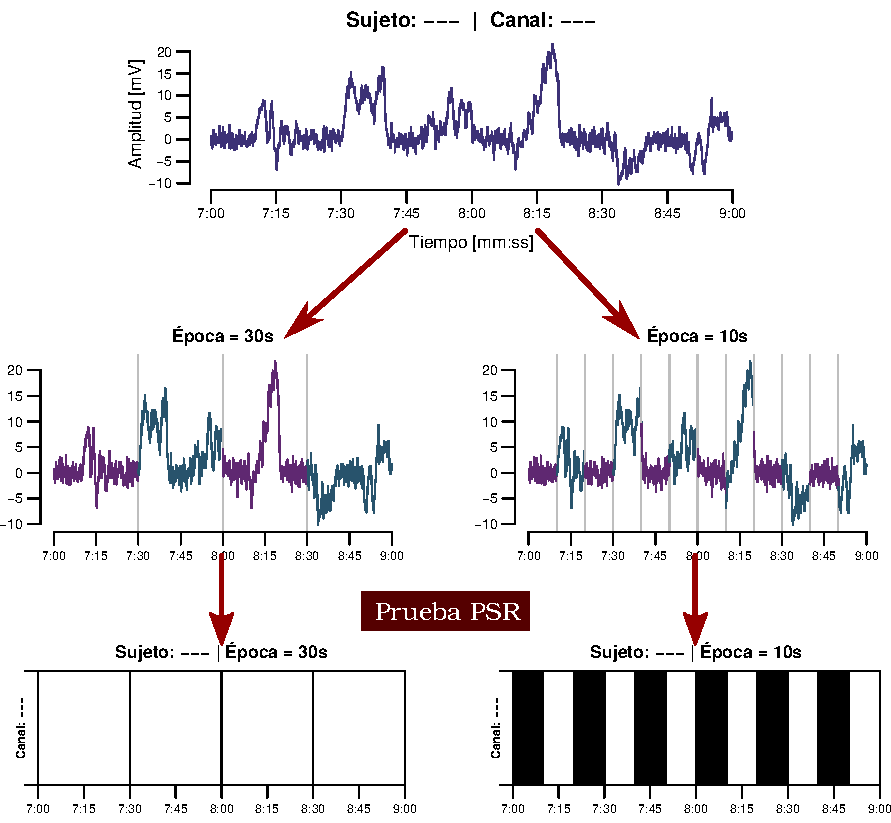
\includegraphics[width=\linewidth]{./img_diagramas/epocas_diferentes_v2.pdf}
\caption{Esquema de cómo se tomaron diferentes tamaños de época para estudiar los registros de 
PSG}
\label{epocas_diferentes}
\end{figure}



%%%%%%%%%%%%%%%%%%%%%%%%%%%%%%%%%%%%%%%%%%%%%%%%%%%%%%%%%%%%%%%%%%%%%%%%%%%%%%%%%%%%%%%%%%%%%%%%%%%
%%%%%%%%%%%%%%%%%%%%%%%%%%%%%%%%%%%%%%%%%%%%%%%%%%%%%%%%%%%%%%%%%%%%%%%%%%%%%%%%%%%%%%%%%%%%%%%%%%%
%%%%%%%%%%%%%%%%%%%%%%%%%%%%%%%%%%%%%%%%%%%%%%%%%%%%%%%%%%%%%%%%%%%%%%%%%%%%%%%%%%%%%%%%%%%%%%%%%%%
%%%%%%%%%%%%%%%%%%%%%%%%%%%%%%%%%%%%%%%%%%%%%%%%%%%%%%%%%%%%%%%%%%%%%%%%%%%%%%%%%%%%%%%%%%%%%%%%%%%

%%%%%%%%%%%%%%%%%%%%%%%%%%%%%%%%%%%%%%%%%%%%%%%%%%%%%%%%%%%%%%%%%%%%%%%%%%%%%%%%%%%%%%%%%%%%%%%%%%%
%%%%%%%%%%%%%%%%%%%%%%%%%%%%%%%%%%%%%%%%%%%%%%%%%%%%%%%%%%%%%%%%%%%%%%%%%%%%%%%%%%%%%%%%%%%%%%%%%%%
%%%%%%%%%%%%%%%%%%%%%%%%%%%%%%%%%%%%%%%%%%%%%%%%%%%%%%%%%%%%%%%%%%%%%%%%%%%%%%%%%%%%%%%%%%%%%%%%%%%
%%%%%%%%%%%%%%%%%%%%%%%%%%%%%%%%%%%%%%%%%%%%%%%%%%%%%%%%%%%%%%%%%%%%%%%%%%%%%%%%%%%%%%%%%%%%%%%%%%%

\chapter{Resultados}

En cada canal que conforma el PSG (EEG, EOG y EMG), cada \'epoca registrada fue clasificada como 
'posiblemente estacionaria' (PE) si, usando la prueba PSR, no pudo rechazarse la hip\'otesis de 
estacionariedad ($\alpha < 0.05$), o como 'no-estacionaria' en caso contrario.
La cantidad de \'epocas PE en cada individuo, durante el sue\~no MOR y NMOR, se muestra en las 
tablas \ref{total_gpos_mor}, \ref{total_gpos_nmor} y \ref{total_gpos_total}. Debido a la gran 
variabilidad entre los sujetos para la duraci\'on del sue\~no MOR, no se consider\'o el total de 
\'epocas PE, sino la proporci\'on de \'estas en cada etapa de sue\~no; tales cantidades se muestran 
en las tablas \ref{gpos_mor}, \ref{gpos_nmor} y \ref{gpos_total}. 
Adicionalmente se han calculado promedios y desviaciones est\'andar para ambos grupos (Control y 
PDC).

\section{Resultados principales}

Como un primer an\'alisis se verific\'o si el sue\~no MOR, entendido como muestra del registro
completo, tiene o no propiedades estad\'isticas parecidas a este \'ultimo, y si \'esta similaridad 
pudiera estar relacionada con el PDC. 
Se compar\'o la proporci\'on de \'epocas PE en cada canal durante sue\~no MOR y NMOR usando la 
prueba $\chi^{2}$ para proporciones\footnote{Implementada en R como la funci\'on 
\texttt{prop.test()}}; estos resultados se muestran en la tabla \ref{comparacion_mor_vs_total},
y son resumidos esquem\'aticamente en la figura \ref{cabecitas_munchas}.

Se encontr\'o que no hay diferencias significativas, consistentes en todos los sujetos, en los 
canales LOG y ROG, lo cual puede ser explicado por la tipificaci\'on del sue\~no MOR. 
Por otro lado, no se encontr\'o una relaci\'on clara entre el estado de salud del sujeto y la 
aparici\'on de diferencias significativas entre estas proporciones.

\begin{figure}
\centering
\begin{tabular}{c}
\begin{tabular}{ccccc}
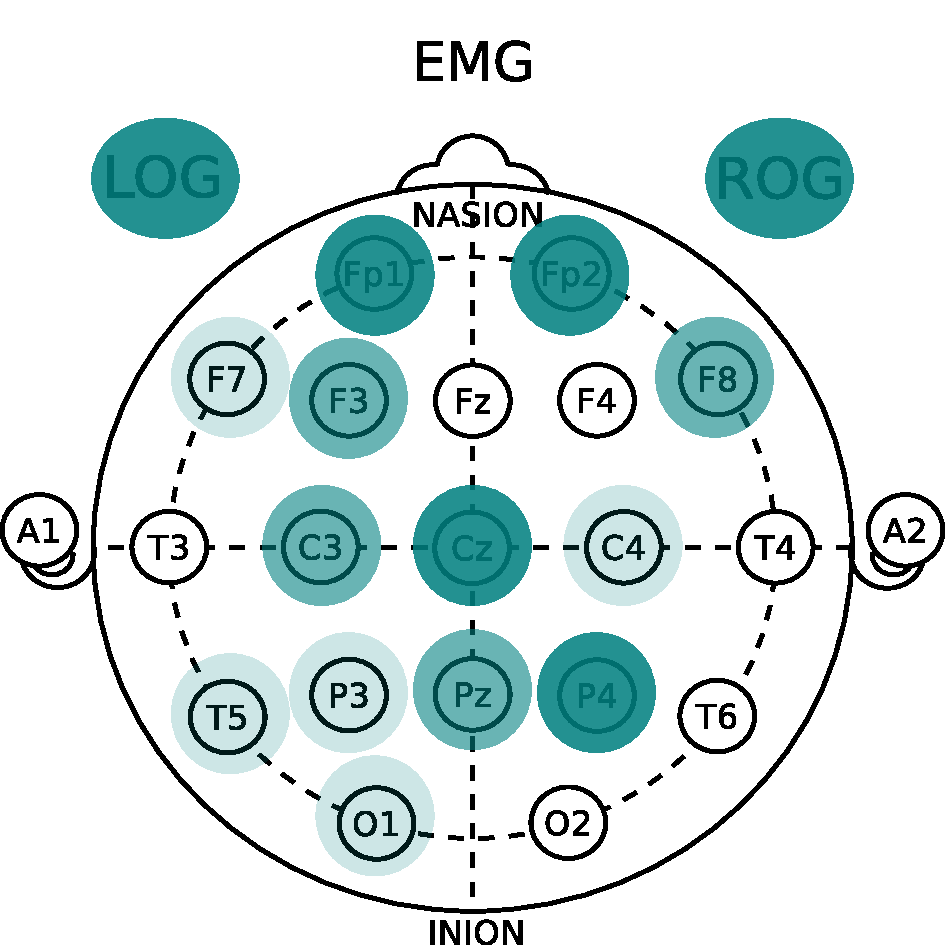
\includegraphics[width=0.17\textwidth]{./img_diagramas/cabecita_VCR.pdf} &
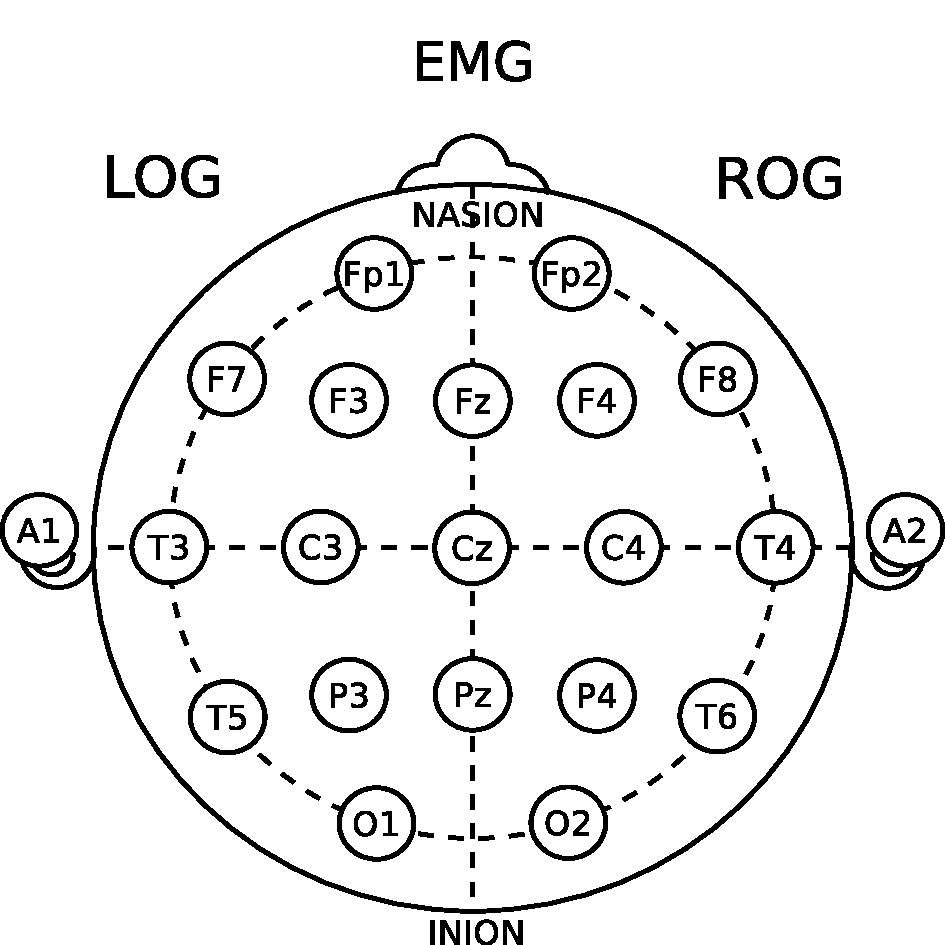
\includegraphics[width=0.17\textwidth]{./img_diagramas/cabecita_MJH.pdf} &
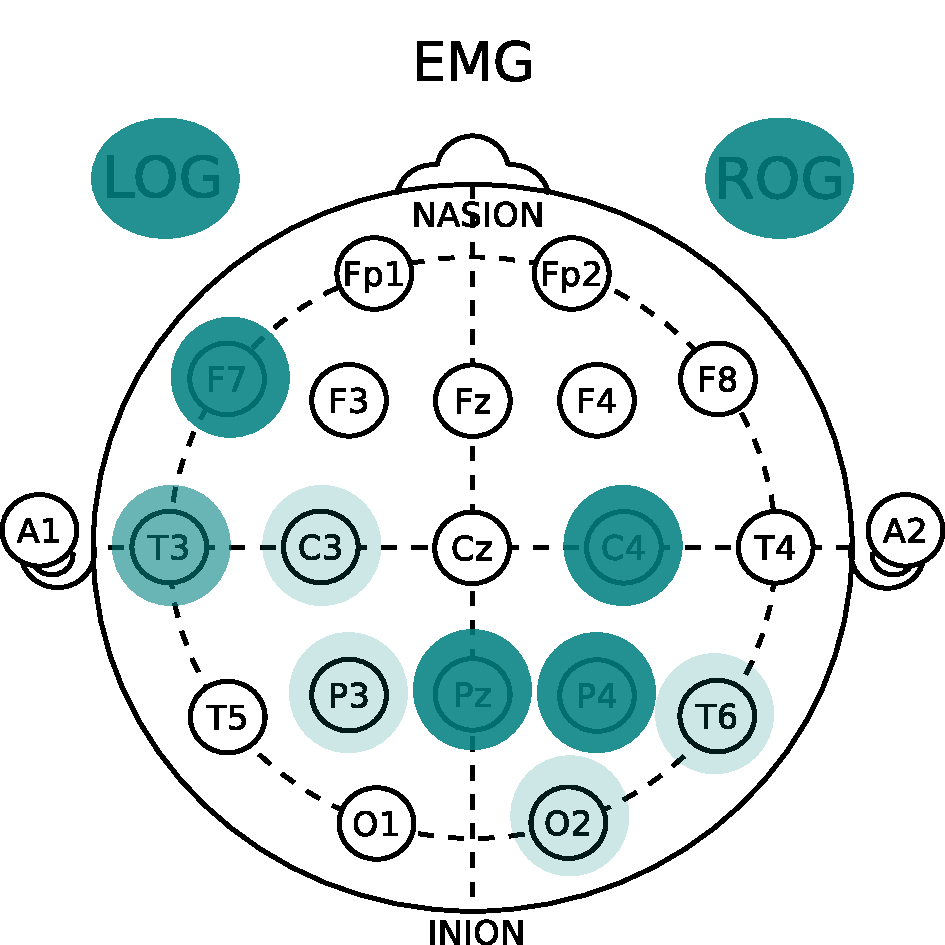
\includegraphics[width=0.17\textwidth]{./img_diagramas/cabecita_JAE.pdf} &
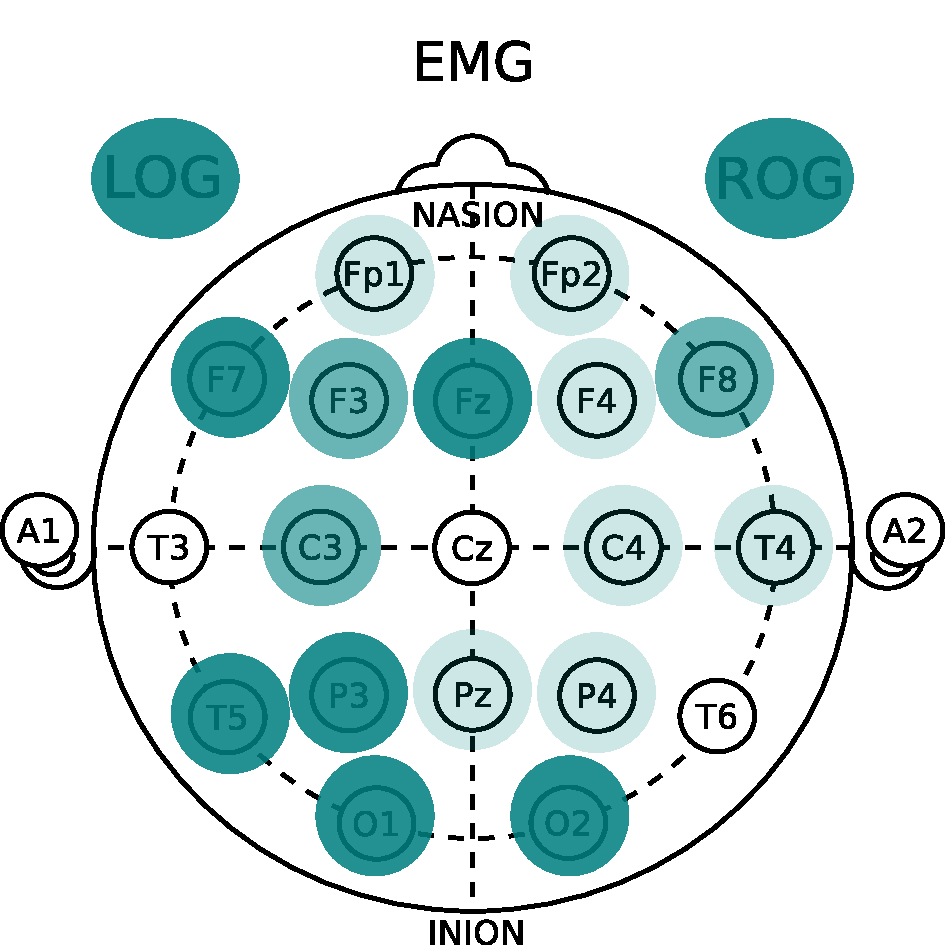
\includegraphics[width=0.17\textwidth]{./img_diagramas/cabecita_GHA.pdf} &
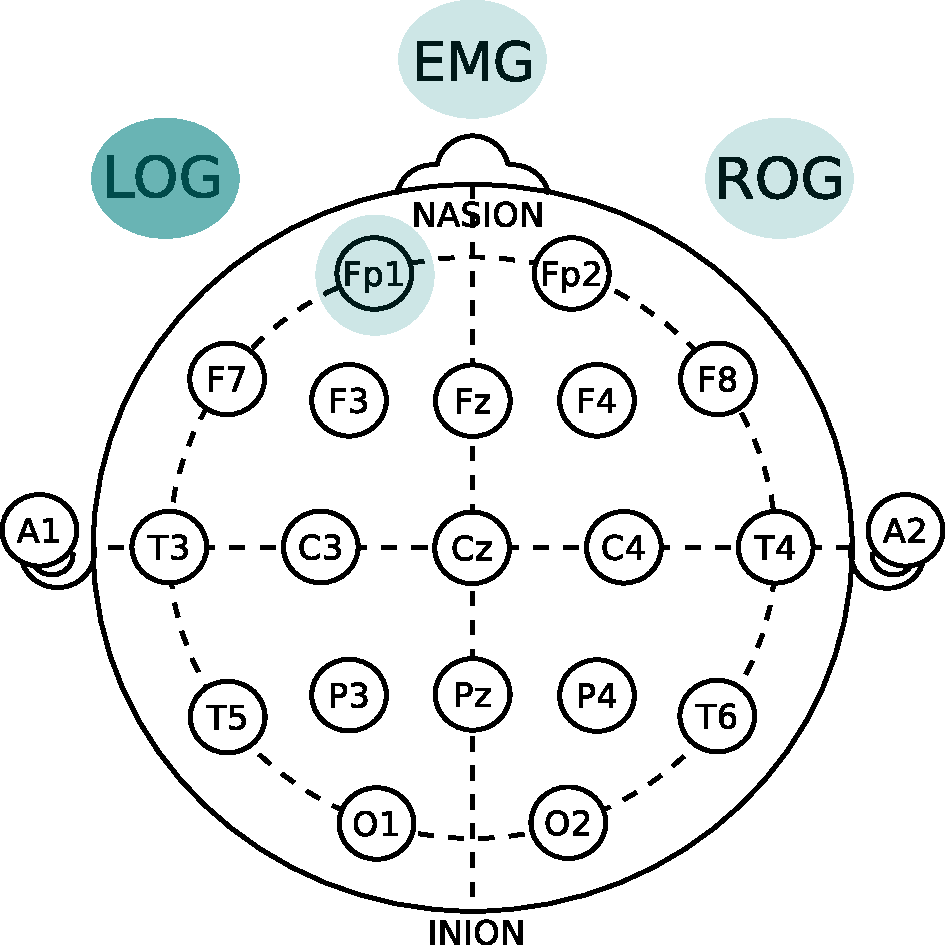
\includegraphics[width=0.17\textwidth]{./img_diagramas/cabecita_MFGR.pdf} \\
VCR & MJH & JAE & GHA & MFGR
\end{tabular}
\\
\begin{tabular}{cccc}
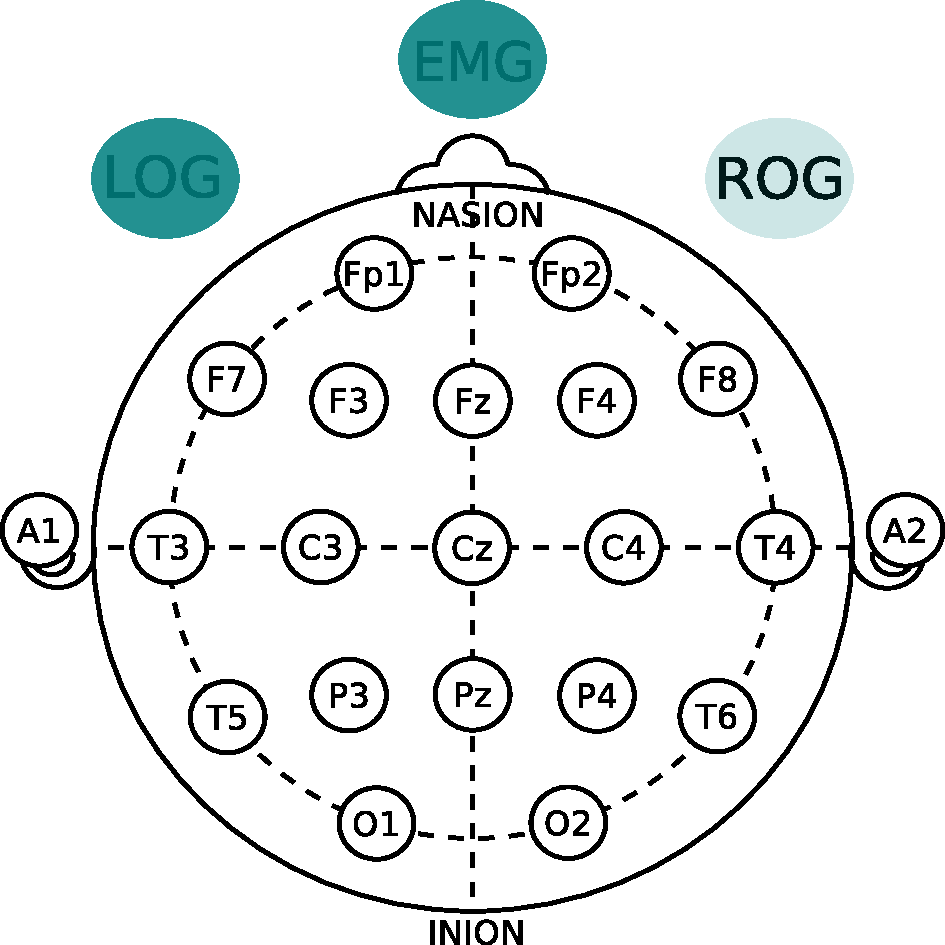
\includegraphics[width=0.17\textwidth]{./img_diagramas/cabecita_CLO.pdf} &
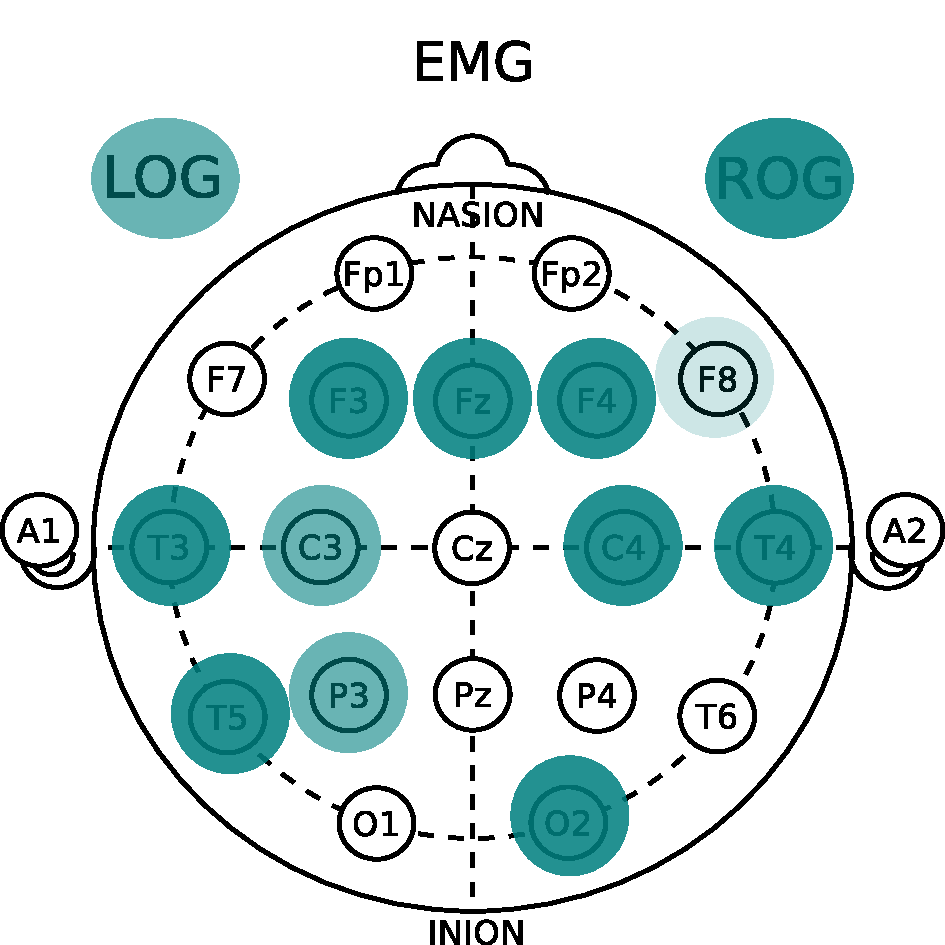
\includegraphics[width=0.17\textwidth]{./img_diagramas/cabecita_RLO.pdf} &
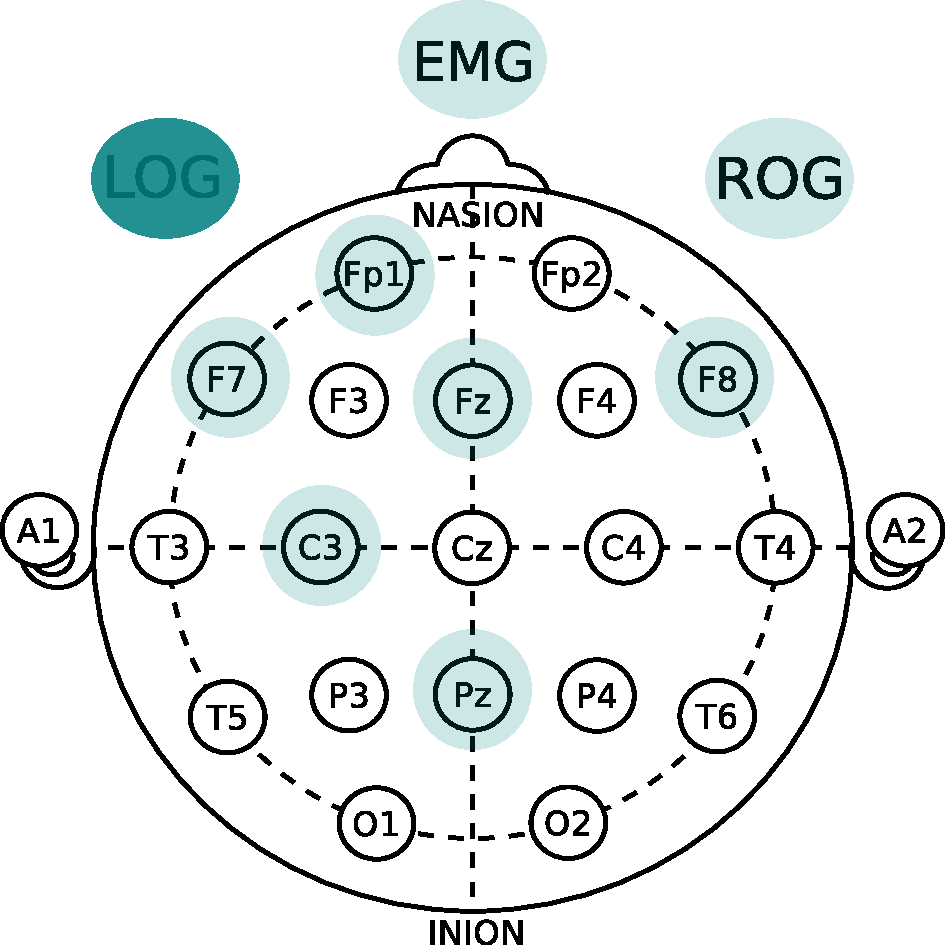
\includegraphics[width=0.17\textwidth]{./img_diagramas/cabecita_RRU.pdf} &
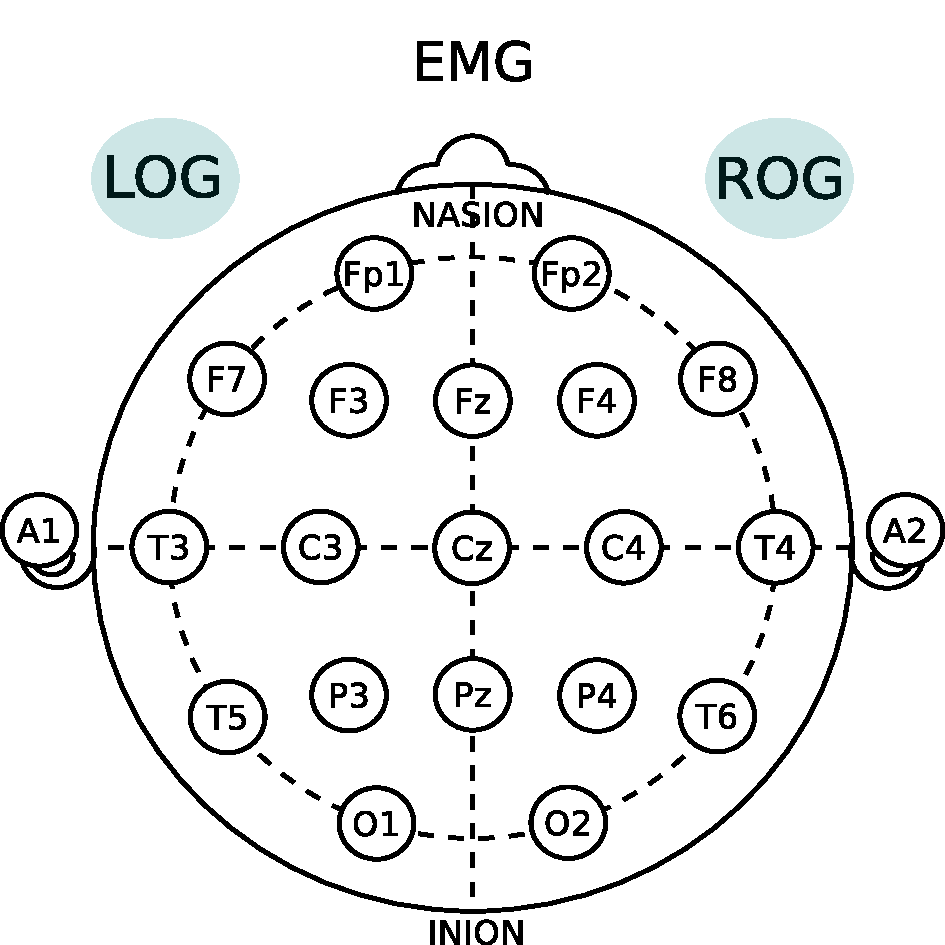
\includegraphics[width=0.17\textwidth]{./img_diagramas/cabecita_JGZ.pdf} \\
CLO & RLO & RRU & JGZ
\end{tabular}
\\
\begin{tabular}{ccc}
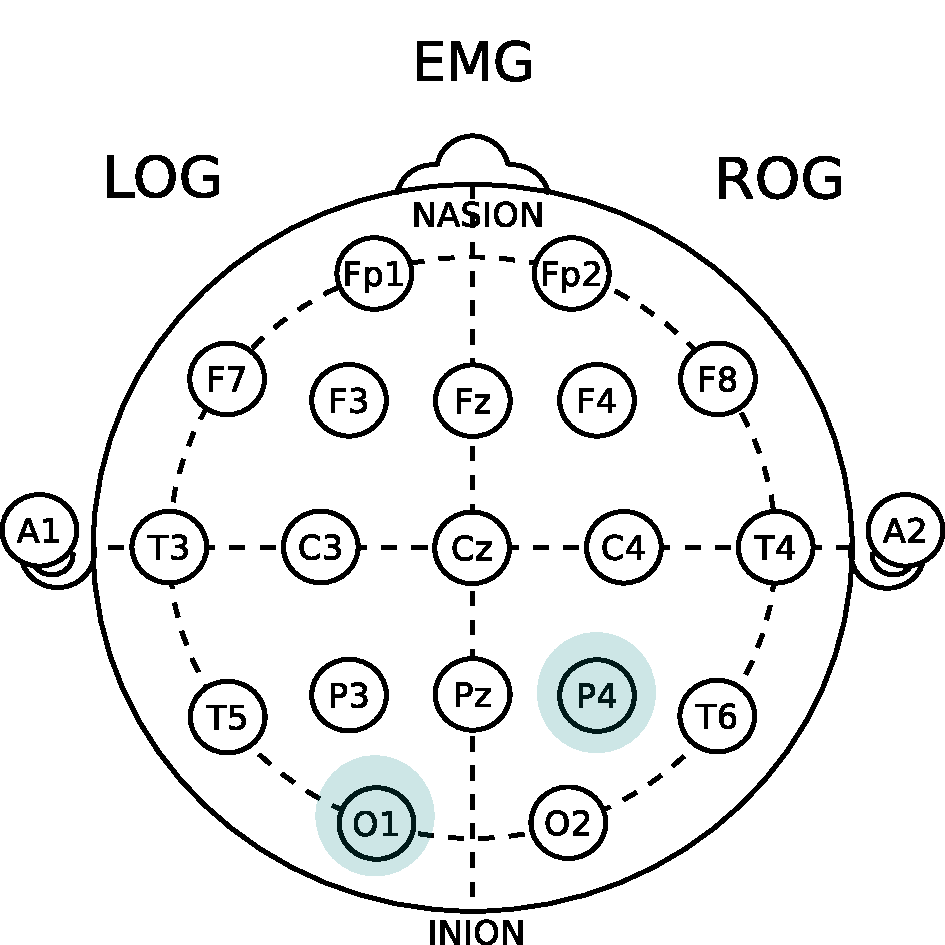
\includegraphics[width=0.17\textwidth]{./img_diagramas/cabecita_FGH.pdf} &
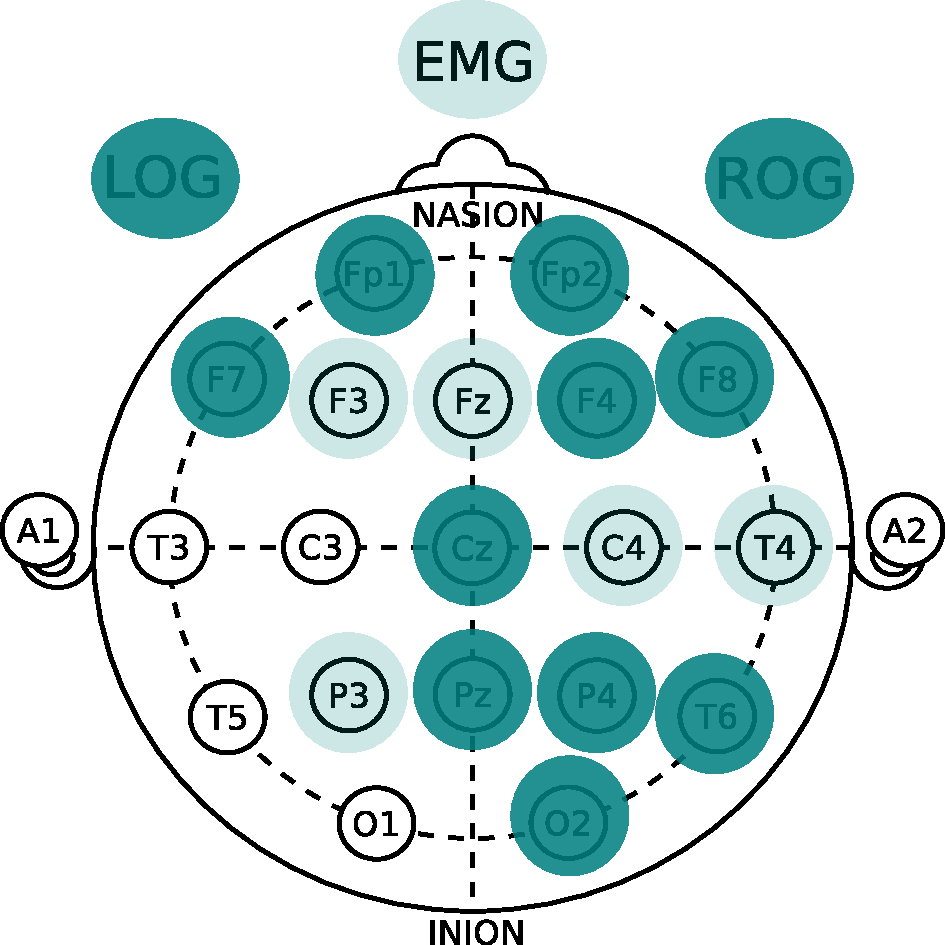
\includegraphics[width=0.17\textwidth]{./img_diagramas/cabecita_MGG.pdf} &
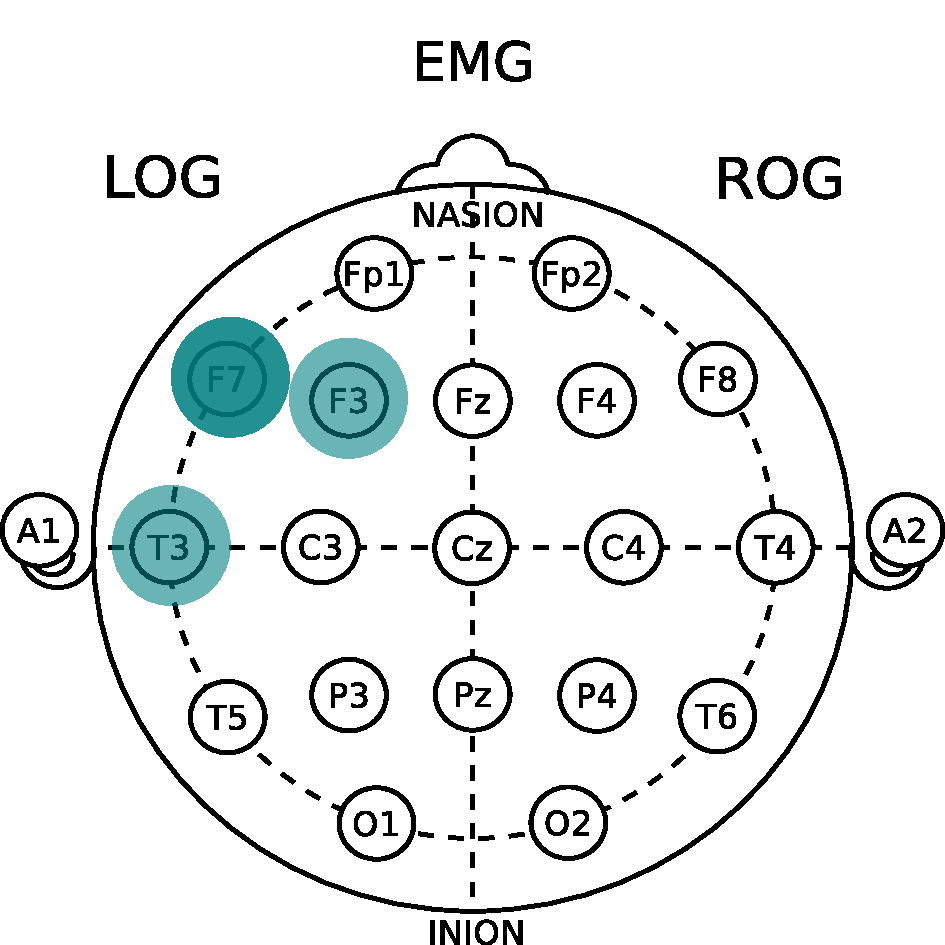
\includegraphics[width=0.17\textwidth]{./img_diagramas/cabecita_EMT.pdf} \\
FGH & MGG & EMT
\end{tabular}
\end{tabular}
\caption{Se muestra esquem\'aticamente en azul las zonas donde se encontraron diferencias 
significativas al comparar las proporciones de \'epocas PE durante sue\~no MOR y NMOR. Esta misma
informaci\'on se muestra en la tabla \ref{comparacion_mor_vs_total} }
\label{cabecitas_munchas}
\end{figure}

Posteriormente se busc\'o una diferencia m\'as directa entre los grupos, comparando grupalmente las 
proporciones de \'epocas PE (en cada canal y durante las diferentes etapas) mediante la prueba U de 
Mann-Whitney\footnote{Implementada en R como la funci\'on \texttt{wilcox.test()}}; no se 
encontraron diferencias significativas para ninguno de los canales. Los resultados se muestran en 
las tablas \ref{gpos_mor}, \ref{gpos_nmor}, \ref{gpos_total}, y para una mejor visualizaci\'on 
\'estos se han graficado en la figura \ref{comparacion_graf}.

\begin{figure}
\centering
\subfloat[Comparaci\'on entre \'epocas MOR (fase R)]{
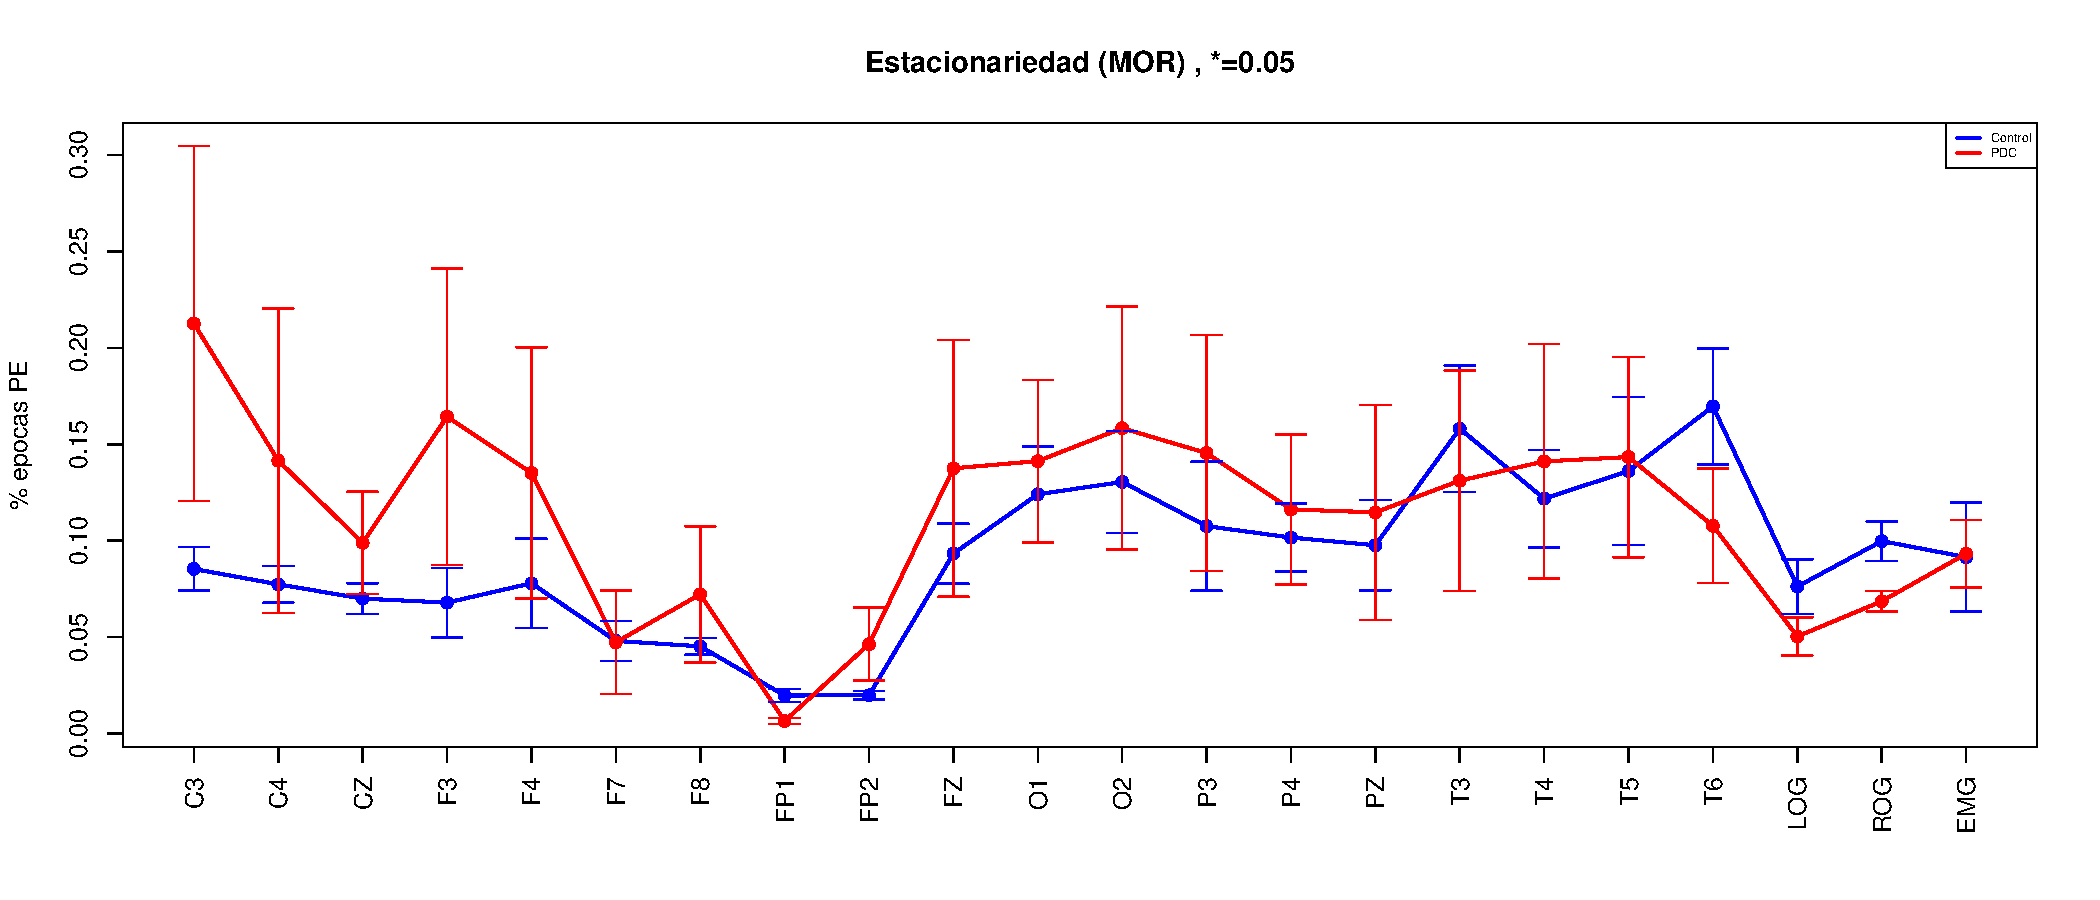
\includegraphics[width=0.95\linewidth]
{./img_ejemplos/Comparacion_gpos_MOR.pdf} 
}\\
\subfloat[Comparaci\'on entre \'epocas no-MOR (fases W y N)]{
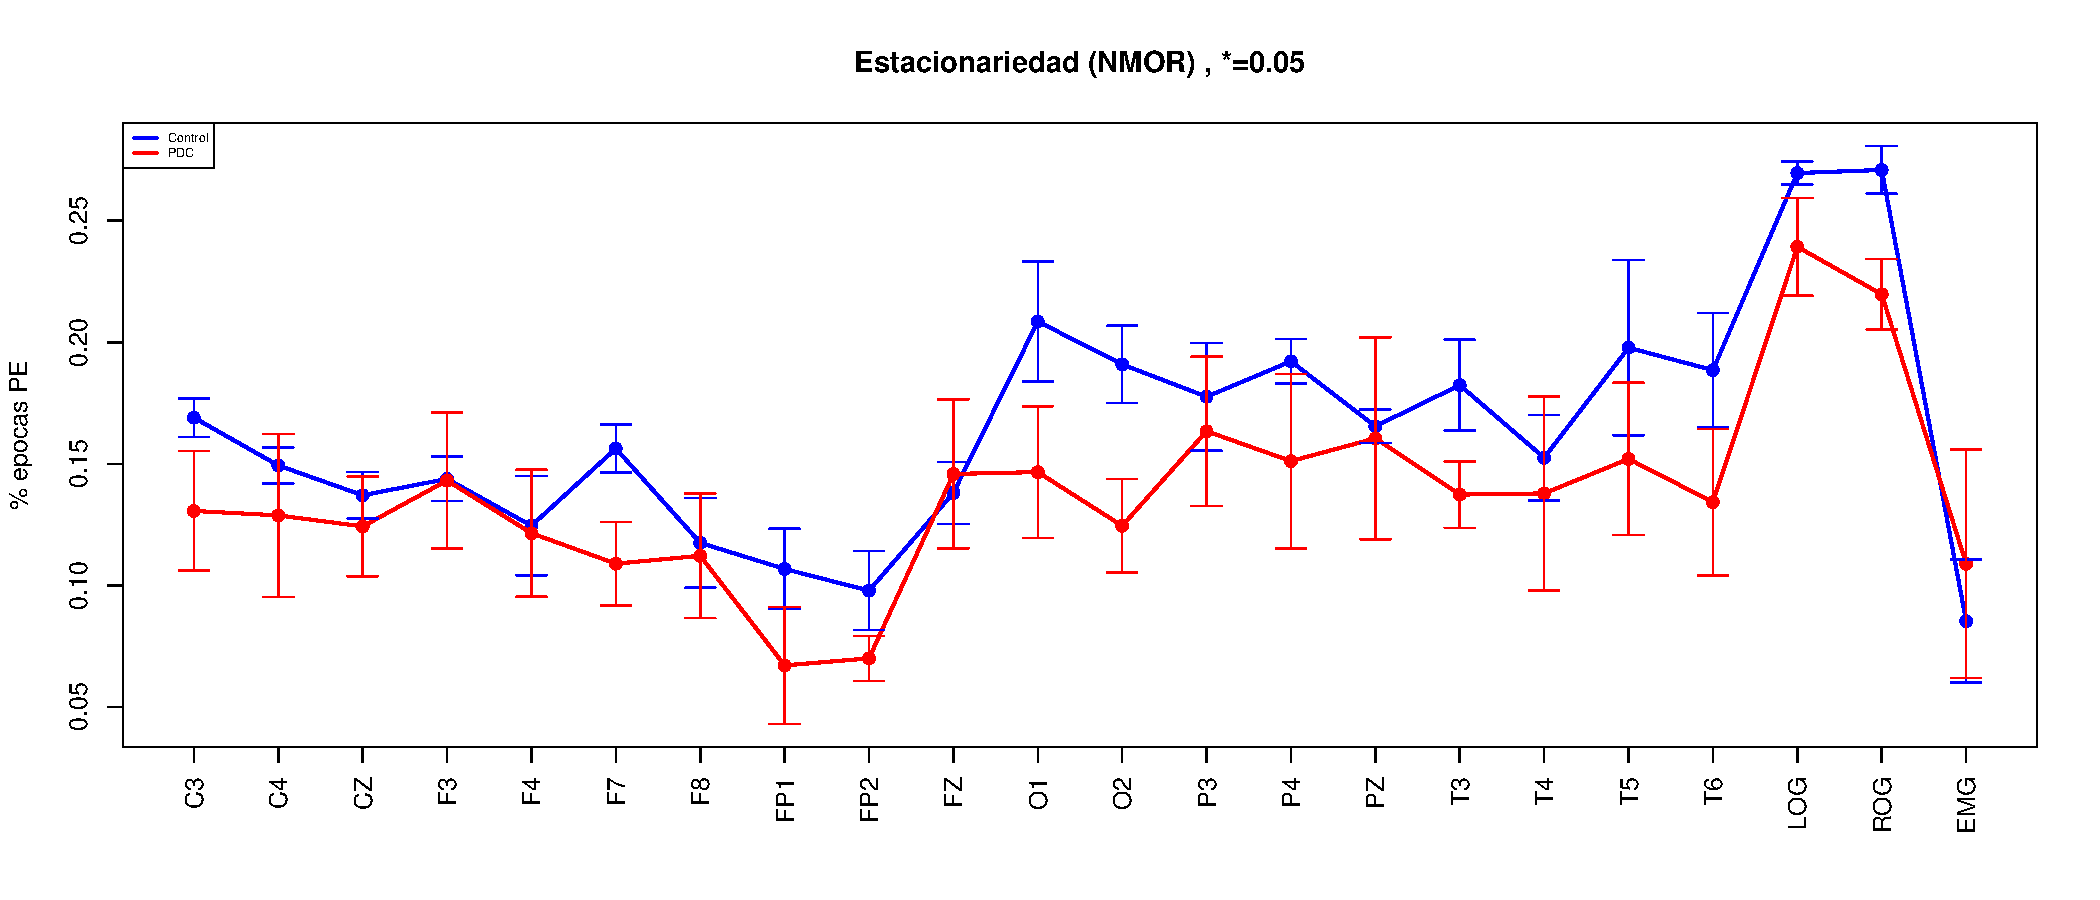
\includegraphics[width=0.95\linewidth]
{./img_ejemplos/Comparacion_gpos_NMOR.pdf} 
}\\
\caption{Comparaci\'on sobre las proporciones de \'epocas PE entre los grupos Control (azul) y PDC 
(rojo), para diferentes etapas de sue\~no (MOR y NMOR). Se grafica el promedio grupal $\pm$ 1 
desviaci\'on est\'andar$^{\nicefrac{3}{2}}$, como visualizaci\'on aproximada de la varianza.}
\label{comparacion_graf}
\end{figure}

Una segunda variaci\'on del primer an\'alisis es considerar grupalmente a los sujetos como 
'unidades' que transitan entre etapas de sue\~no; se comparan grupalmente las proporciones de 
\'epocas PE en cada canal durante sue\~no MOR y NMOR, usando la prueba U de Mann-Whithney; en 
la figura \ref{comparacion_verde} se han representado gr\'aficamente estas diferencias.
Se encontr\'o que hay diferencias significativas ($\alpha<0.1$) para el grupo Control en los 
canales C3, C4, F7, F8, FP1, FP2, O2, P4, LOG y ROG, mientras que en el grupo PDC s\'olo se
observaron diferencias en LOG y ROG.
Descartando los canales LOG y ROG, ya que no son parte del EEG, las diferencias encontradas pueden 
ser relevantes fisiol\'ogicamente, ya que abarcan gran parte de los l\'obulos frontal y parietal, 
y parte de la regi\'on occipital-parietal derecha; en la figura \ref{cabecita} se indican 
esquem\'aticamente estas regiones.

\begin{figure}
\centering
\subfloat[Comparaci\'on para el grupo control]{
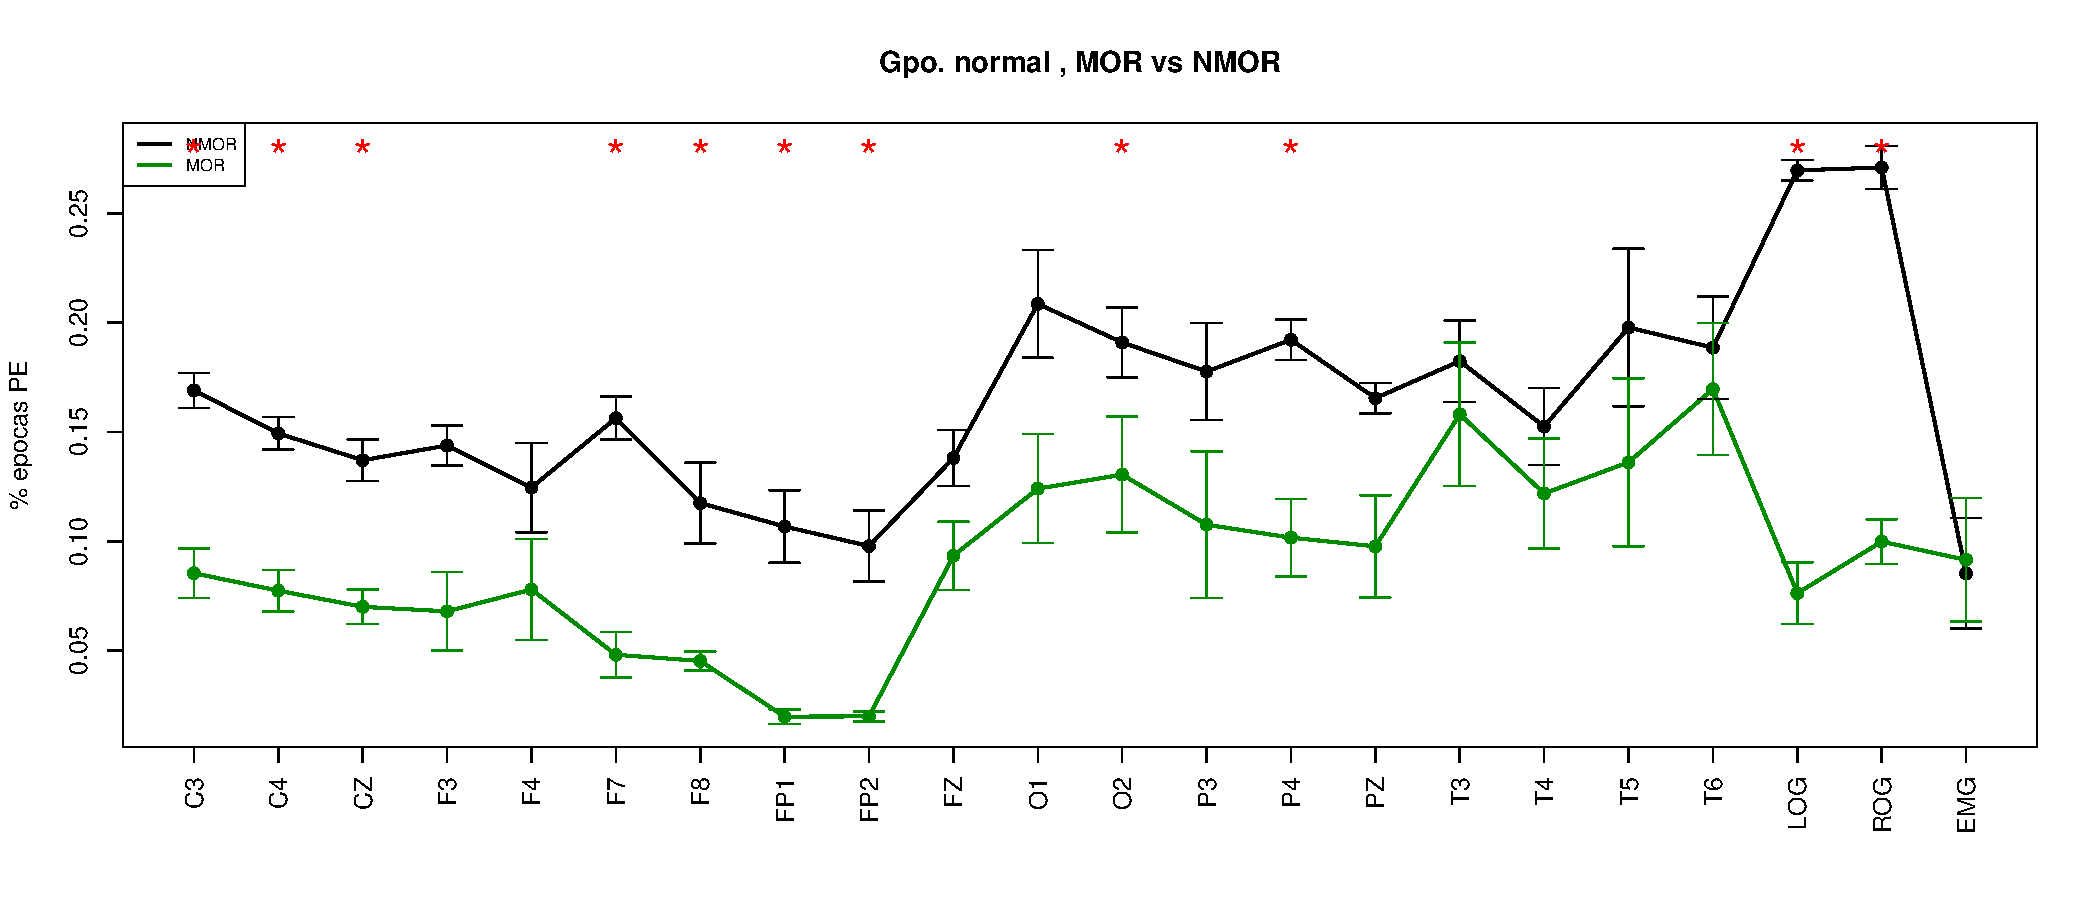
\includegraphics[width=0.95\linewidth]
{./img_ejemplos/comp_etapas_gpos_NORMALMOR_vs_NMOR.pdf} 
}\\
\subfloat[Comparaci\'on para el grupo PDC]{
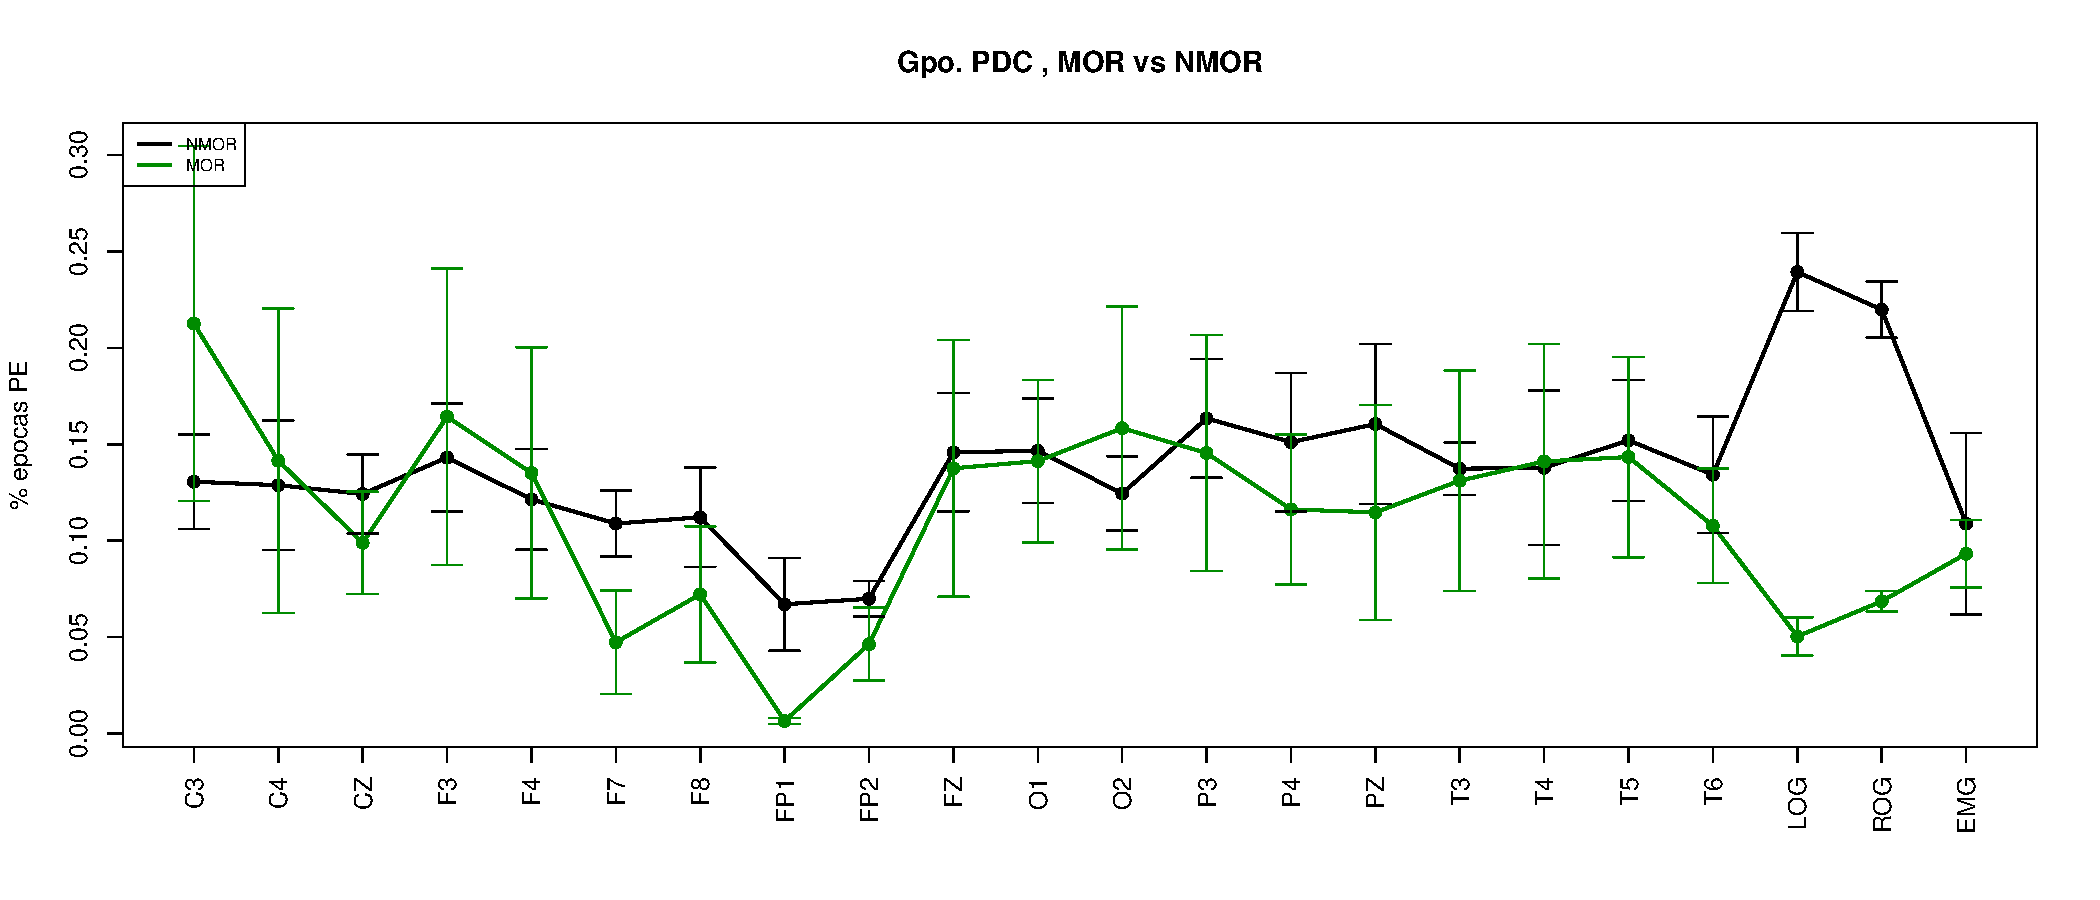
\includegraphics[width=0.95\linewidth]
{./img_ejemplos/comp_etapas_gpos_PDCMOR_vs_NMOR.pdf} 
}
\caption{Comparaci\'on sobre las proporciones de \'epocas PE entre las etapas de sue\~no MOR 
(verde) y NMOR (negro), para ambos grupos por separado. Se han graficado las proporciones de PE en 
todos los sujetos de cada grupo, para todo el sue\~no y la etapa MOR.
Se grafica el promedio grupal $\pm$ 1 desviaci\'on est\'andar$^{\nicefrac{3}{2}}$, como 
visualizaci\'on aproximada de la varianza.}
\label{comparacion_verde}
\end{figure}

\begin{figure}
\centering
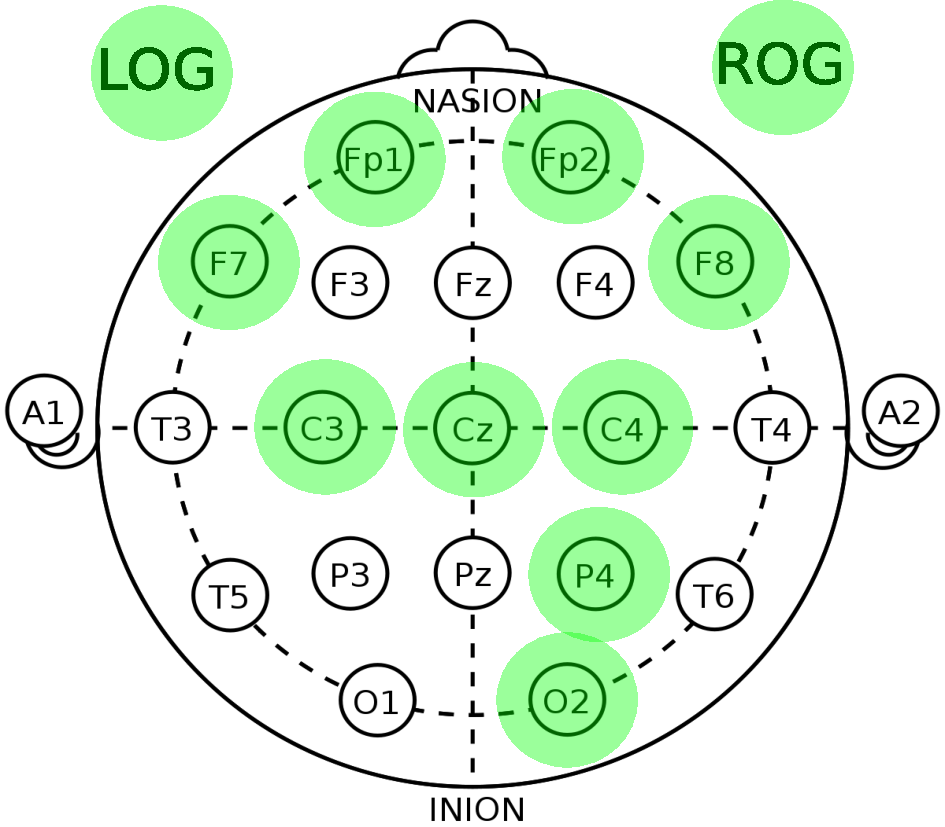
\includegraphics[width=0.4\linewidth]
{./img_diagramas/cabecita.pdf} 
\caption{Representaci\'on esquem\'atica de los sitios donde se encontraron diferencias 
significativas en la comparaci\'on entre el porcentaje de \'epocas PE durante sue\~no MOR y NMOR, 
para el grupo Control (ver texto)}
\label{cabecita}
\end{figure}

%%%%%%%%%%%%%%%%%%%%%%%%%%%%%%%%%%%%%%%%%%%%%%%%%%%%%%%%%%%%%%%%%%%%%%%%%%%%%%%%%%%%%%%%%%%%%%%%%%%
%%%%%%%%%%%%%%%%%%%%%%%%%%%%%%%%%%%%%%%%%%%%%%%%%%%%%%%%%%%%%%%%%%%%%%%%%%%%%%%%%%%%%%%%%%%%%%%%%%%

\section{Patrones visuales}

Como un an\'alisis exploratorio, buscando explicar la variabilidad entre los resultados, se 
graficaron los resultados obtenidos con la prueba PSR de la siguiente manera: se colocan en 
l\'inea horizontal una serie de cuadros, uno por cada \'epoca analizada seg\'un fue clasificada 
(blanco: PE, negro: no-estacionario), y posteriormente se juntaron verticalmente las l\'ineas
correspondientes a los diferentes canales; en la figura \ref{ejemplo_graf} se muestra un ejemplo de
ello, mientras que en el anexo se muestran los gr\'aficos construidos para cada uno de los sujetos. 

Al construir estos gr\'aficos, se hacen presentes 'bloques' de \'epocas que en su mayor\'ia son
PE --similarmente con \'epocas no-estacionarias. Ha parecido conveniente reportar este hallazgo
ya que los patrones son consistentes en todos los sujetos, y porque parece que estos 'bloques'
aparecen asociados al sue\~no MOR en cierto orden (ilustrado en la figura \ref{patroncito}):
\begin{itemize}
\item Bloque abundante en \'epocas PE, visualmente oscuro
\item Bloque abundante en \'epocas no-estacionarias, visualmente claro
\item Secci\'on que contiene el sue\~no MOR, los canales LOG y ROG muestran son visualmente m\'as
abundante en \'epocas no-estacionarias en esta zona del tiempo
\end{itemize}

\begin{figure}
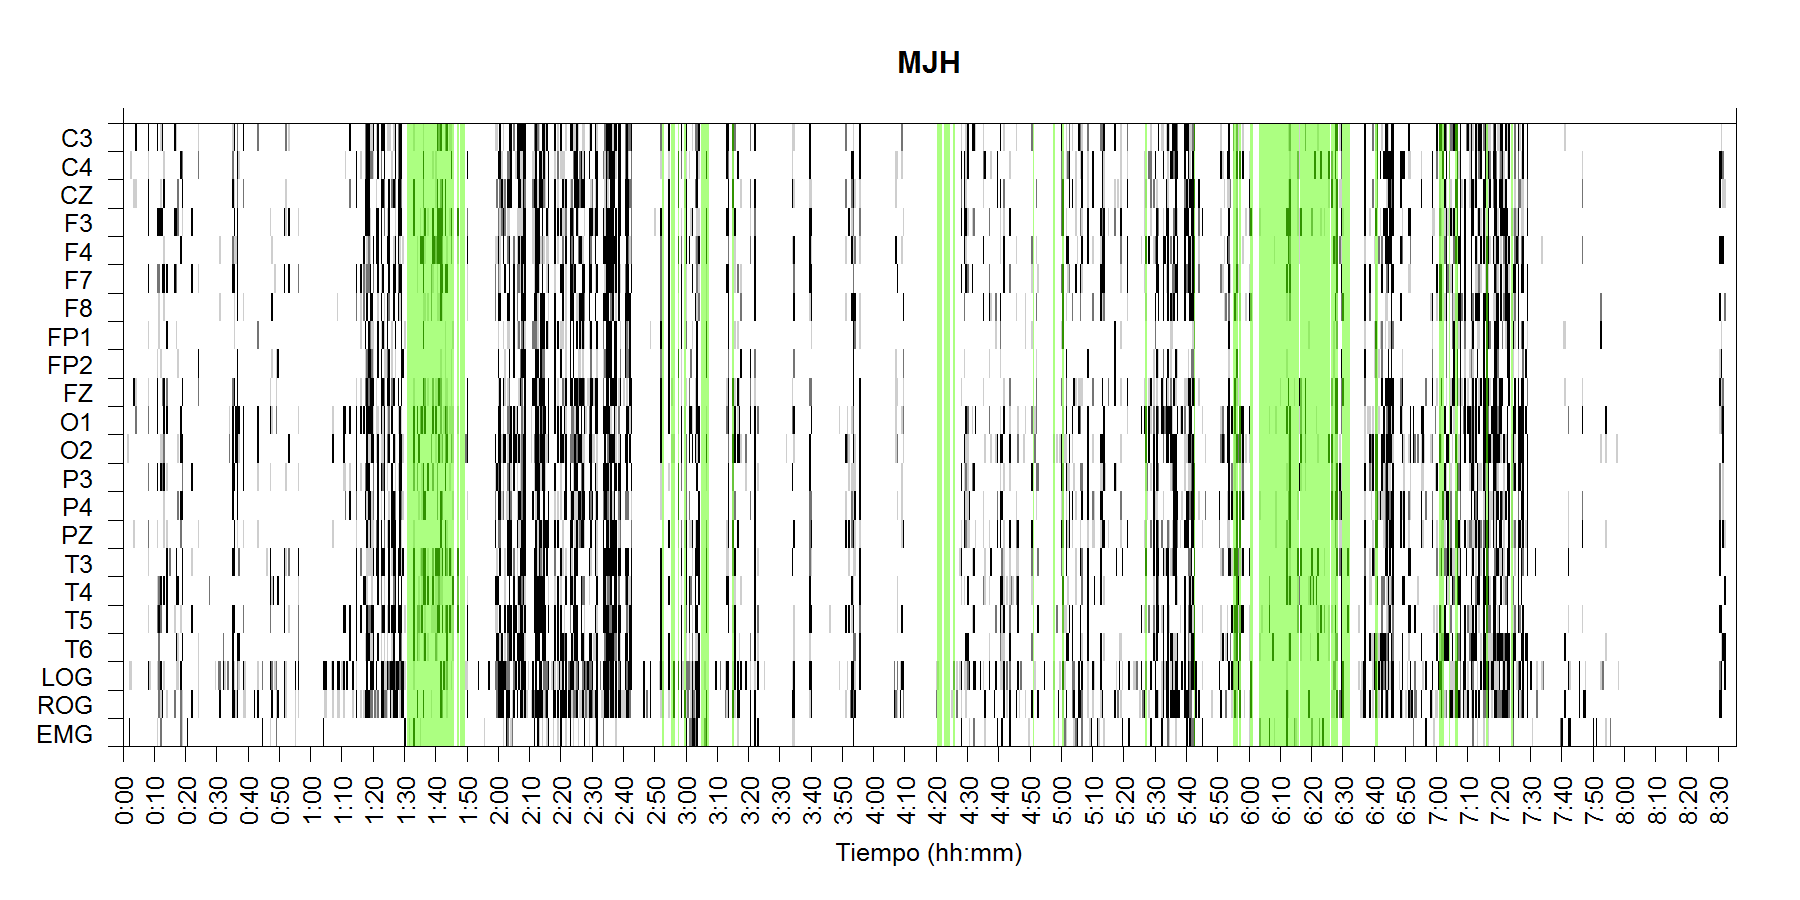
\includegraphics[width=\textwidth]
{./img_ejemplos/MJNNVIGILOS_est.png}
\caption{Disposici\'on gr\'afica para los resultados de la prueba PSR en el sujeto MJH. Se han 
resaltado con color verde las \'epocas clasificadas como de sue\~no MOR.}
\label{ejemplo_graf}
\end{figure}

\begin{figure}
\begin{tabular}{c}
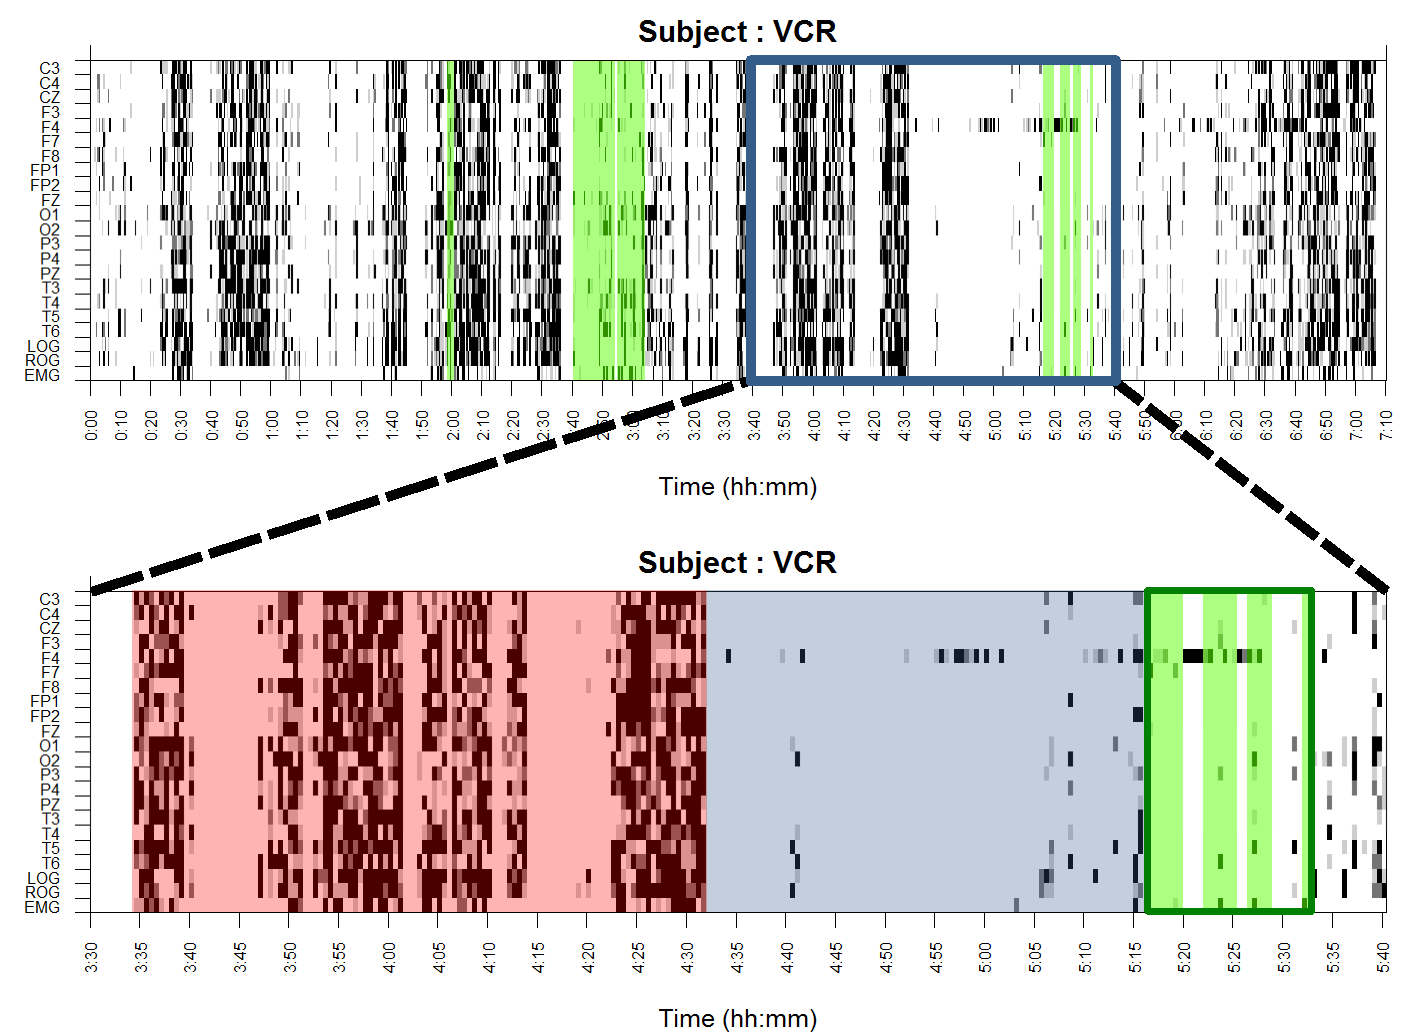
\includegraphics[width=0.3\textwidth]
{./img_ejemplos/zoom_VCR.pdf}
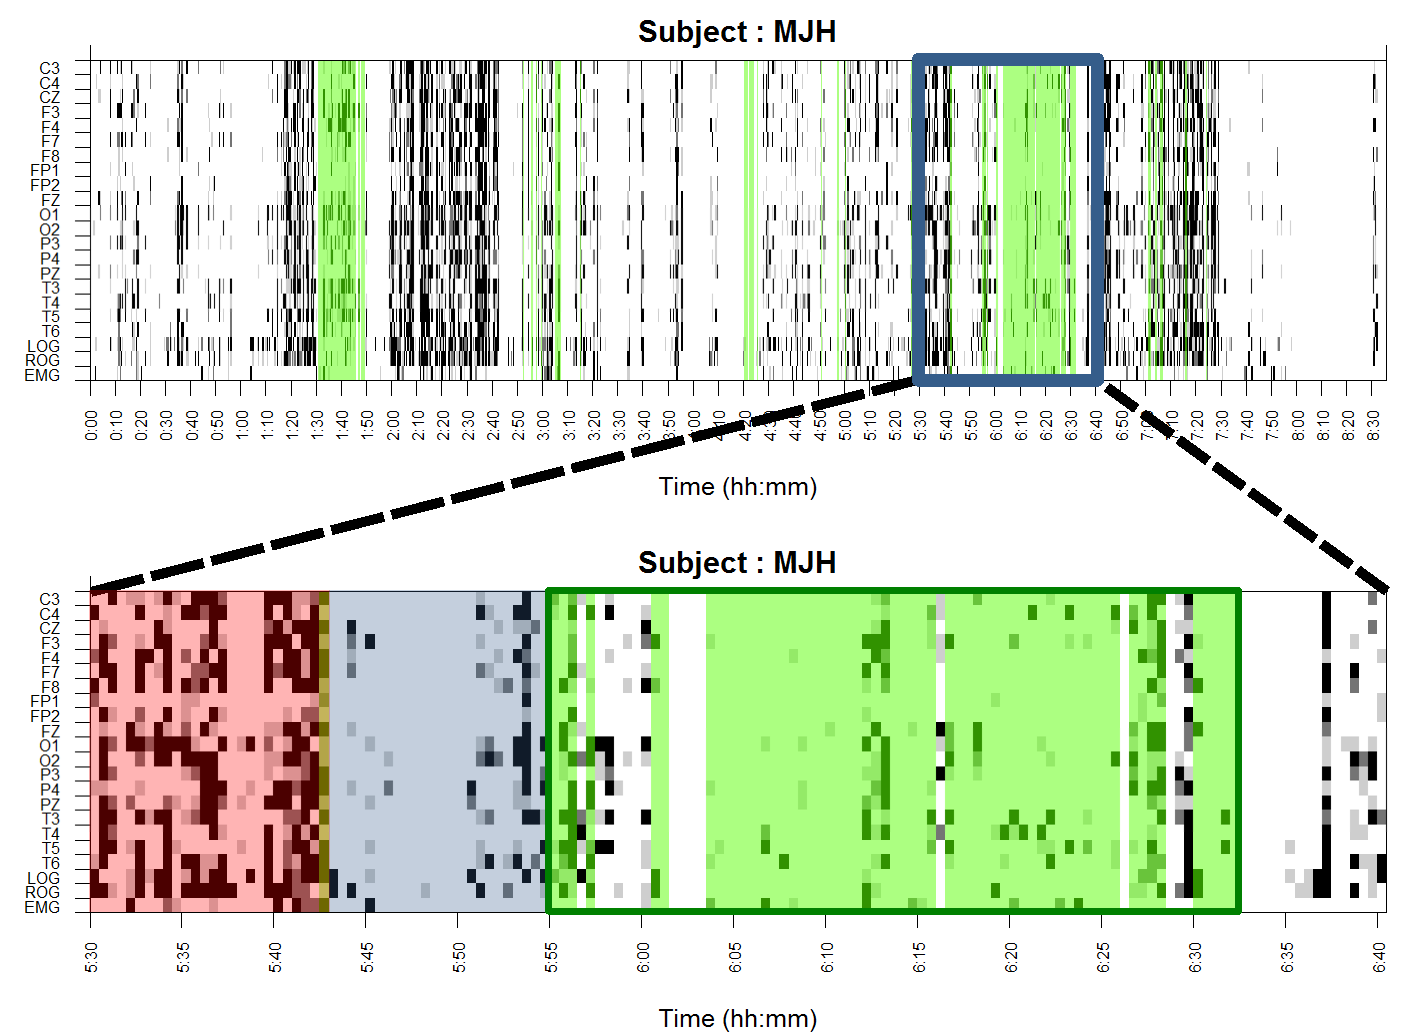
\includegraphics[width=0.3\textwidth]
{./img_ejemplos/zoom_MJH.pdf}
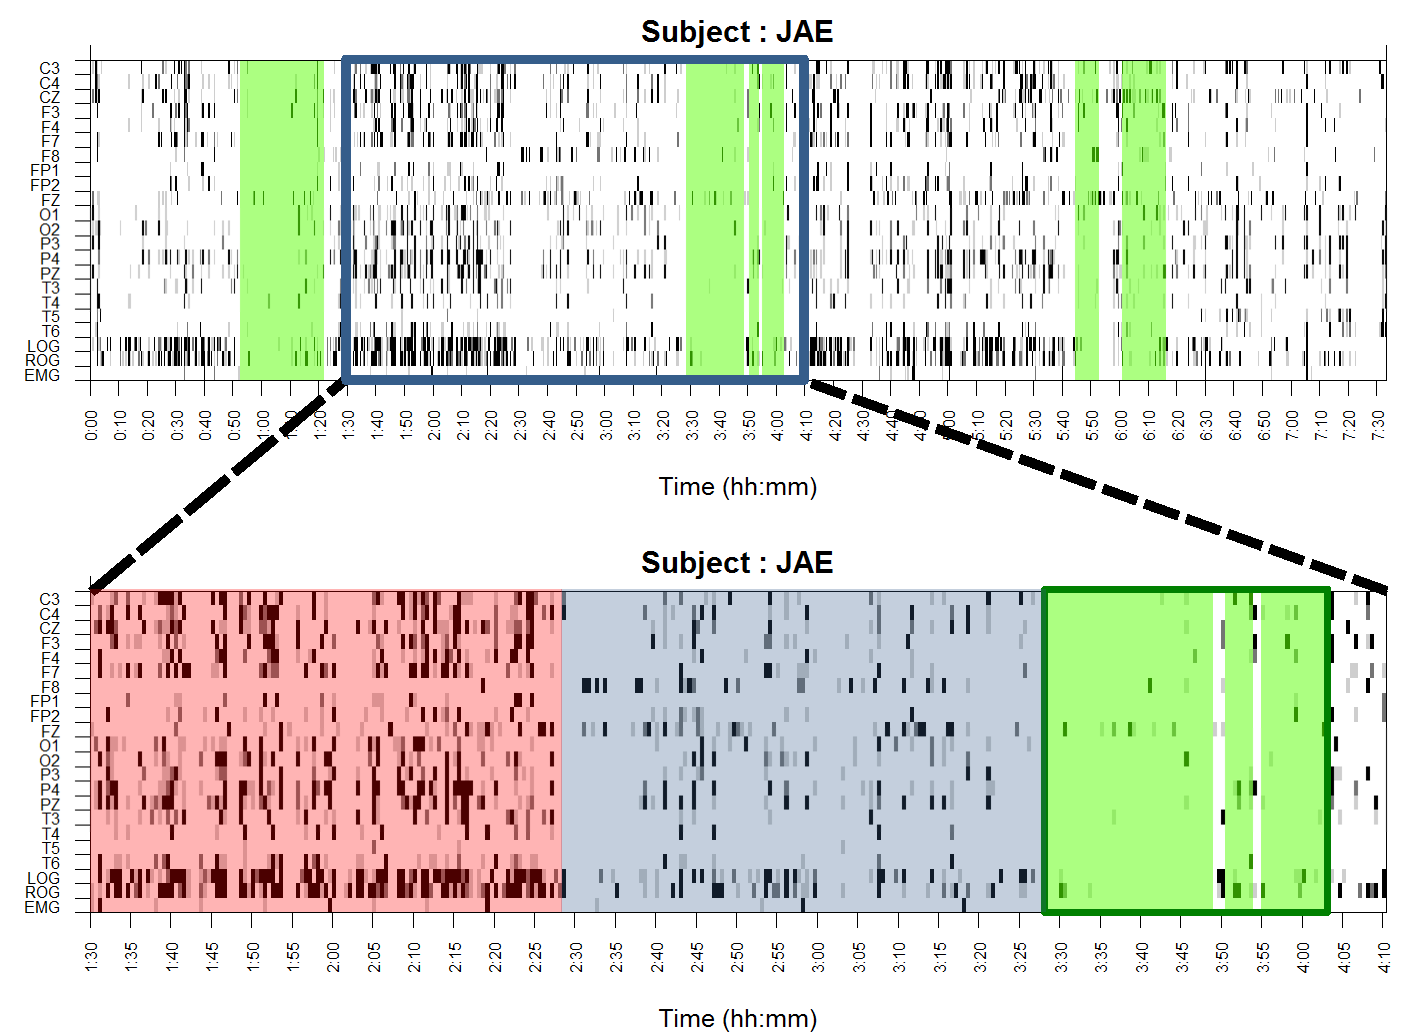
\includegraphics[width=0.3\textwidth]
{./img_ejemplos/zoom_JAE.pdf}
\\
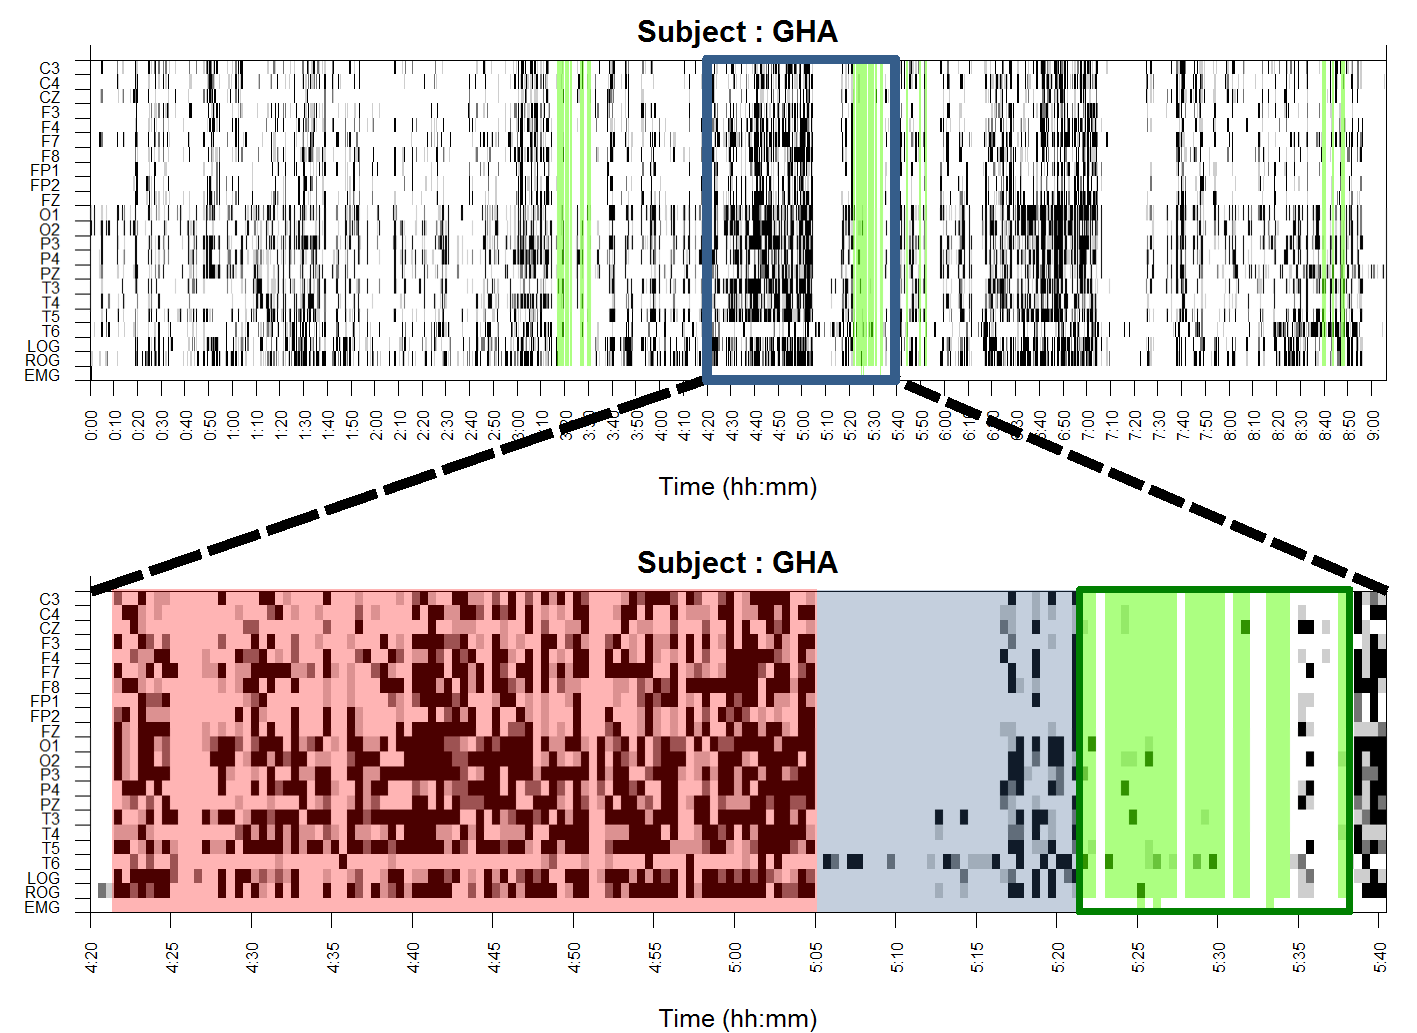
\includegraphics[width=0.3\textwidth]
{./img_ejemplos/zoom_GHA.pdf}
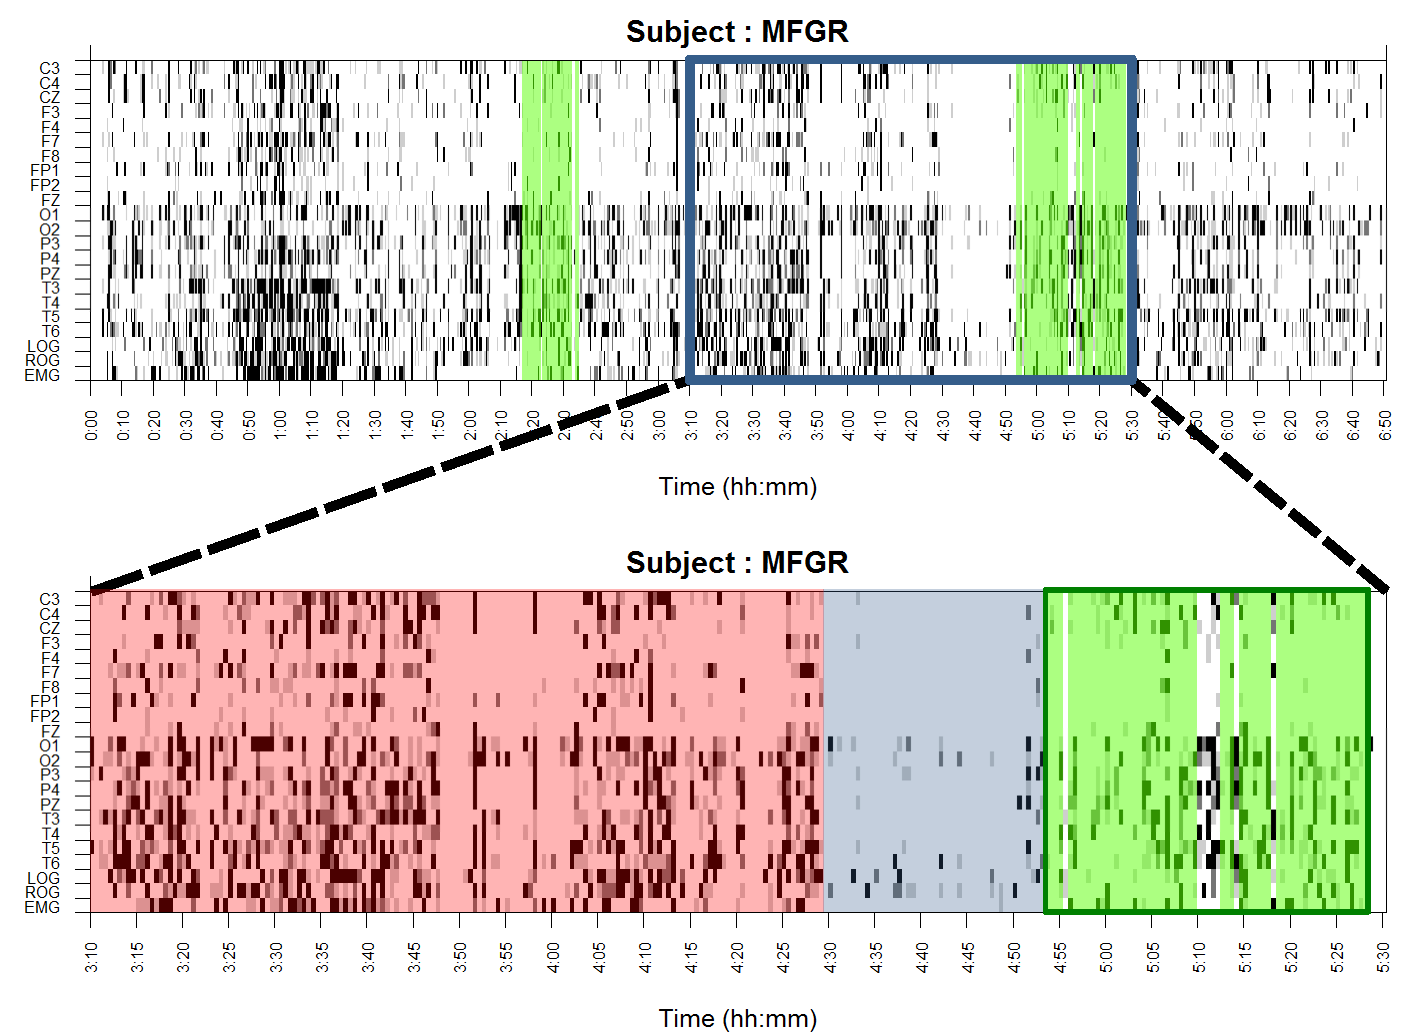
\includegraphics[width=0.3\textwidth]
{./img_ejemplos/zoom_MFGR.pdf}
\end{tabular}
\caption{Ejemplos de los patrones visuales que, se propone, est\'a asociado con la aparici\'on del
sue\~no MOR: un bloque de \'epocas PE (rojo), un bloque de \'epocas no-estacionarias (azul) y un 
bloque que contiene al sue\~no MOR. En este ejemplo se ilustra uno de estos patrones por cada
uno de los sujetos del grupo Control.}
\label{patroncito}
\end{figure}

%%%%%%%%%%%%%%%%%%%%%%%%%%%%%%%%%%%%%%%%%%%%%%%%%%%%%%%%%%%%%%%%%%%%%%%%%%%%%%%%%%%%%%%%%%%%%%%%%%%
%%%%%%%%%%%%%%%%%%%%%%%%%%%%%%%%%%%%%%%%%%%%%%%%%%%%%%%%%%%%%%%%%%%%%%%%%%%%%%%%%%%%%%%%%%%%%%%%%%%
%%%%%%%%%%%%%%%%%%%%%%%%%%%%%%%%%%%%%%%%%%%%%%%%%%%%%%%%%%%%%%%%%%%%%%%%%%%%%%%%%%%%%%%%%%%%%%%%%%%
%%%%%%%%%%%%%%%%%%%%%%%%%%%%%%%%%%%%%%%%%%%%%%%%%%%%%%%%%%%%%%%%%%%%%%%%%%%%%%%%%%%%%%%%%%%%%%%%%%%

\section{Discusi\'on}

Como se mencion\'o anteriormente, este trabajo parte del supuesto en que los sujetos con PDC 
presentan con mayor probabilidad estacionariedad d\'ebil en sus registros de EEG.
Se ha aportado evidencia para afirmar que, al comparar sujetos del grupo Control y con PDC, no hay 
cambios significativos en la porci\'on de tiempo durante la cual el registro de PSG se comporta 
como d\'ebilmente estacionario. 
Esto puede interpretarse como que, quiz\'a, los mecanismos afectados durante el PDC no provocan que 
la se\~nal se vuelva m\'as 'simple' (en el sentido de ser estacionaria).

Cabe un comentario sobre c\'omo la evidencia presentada exhibe al PSG como un conjunto de se\~nales 
no-estacionarias durante la mayor parte del sue\~no, como se suele suponer en se\~nales de origen 
biol\'ogico; entonces, no es adecuado analizar este tipo de se\~nales con m\'etodos que supongan 
estacionariedad, como la estimaci\'on del espectro de potencias usando el periodograma 'cl\'asico'. 

%%%%%%%%%%%%%%%%%%%%%%%%%%%%%%%%%%%%%%%%%%%%%%%%%%%%%%%%%%%%%%%%%%%%%%%%%%%%%%%%%%%%%%%%%%%%%%%%%%%
%%%%%%%%%%%%%%%%%%%%%%%%%%%%%%%%%%%%%%%%%%%%%%%%%%%%%%%%%%%%%%%%%%%%%%%%%%%%%%%%%%%%%%%%%%%%%%%%%%%

\subsection{Sobre los sujetos excluidos}

Durante el trabajo se mencionan tres sujetos (FGH, MGG, EMT) cuyos registros de PSG fueron 
analizados pero que no son considerados estad\'isticamente; cada uno de ellos fue excluido, por 
diversos motivos, del trabajo por V\'azquez Tagle y colaboradores \cite{VazquezTagle16}, pero 
dieron su consentimiento informado para el registro de PSG, debido a lo cual analiz\'o el efecto de 
su inclusi\'on dentro de los an\'alisis.
Destaca el sujeto FGH, quien padece de par\'alisis facial, cataratas, y problemas no especificados 
en hipotiroides y columna; seg\'un se reporta, el sujeto no inform\'o de estos \'ultimos 
padecimientos sino hasta despu\'es del registro de PSG, por lo que su exclusi\'on se efectu\'o a 
posteriori.

Un vistazo a los registros 'inusuales' de FGH (figura\ref{FGH_psg}, comparar con 
\ref{ejemplos_mor}) pudiera haber advertido que en el registro no hay actividad cerebral en los 
canales correspondientes a la regi\'on izquierda (aquella con par\'alisis) sino ruido amplificado 
del polisomn\'ografo.
Dentro del marco de este trabajo, destacan las proporciones inusuales de \'epocas PE (cercanas a 1 
o 0) para este sujeto en los canales F4, F7, F8, FP1, FP2, FZ, tanto en sue\~no MOR como NMOR; 
usando la representaci\'on gr\'afica para FGH, es visible una inusual ausencia total de 
estacionariedad en tales canales (figura \ref{FGH_especial}, comparar con \ref{ejemplo_graf}). 
Si bien esta metodolog\'ia no se dise\~n\'o para tal fin, a\'un as\'i se pudo detectar la falta de 
actividad cerebral.

\begin{figure}
\centering
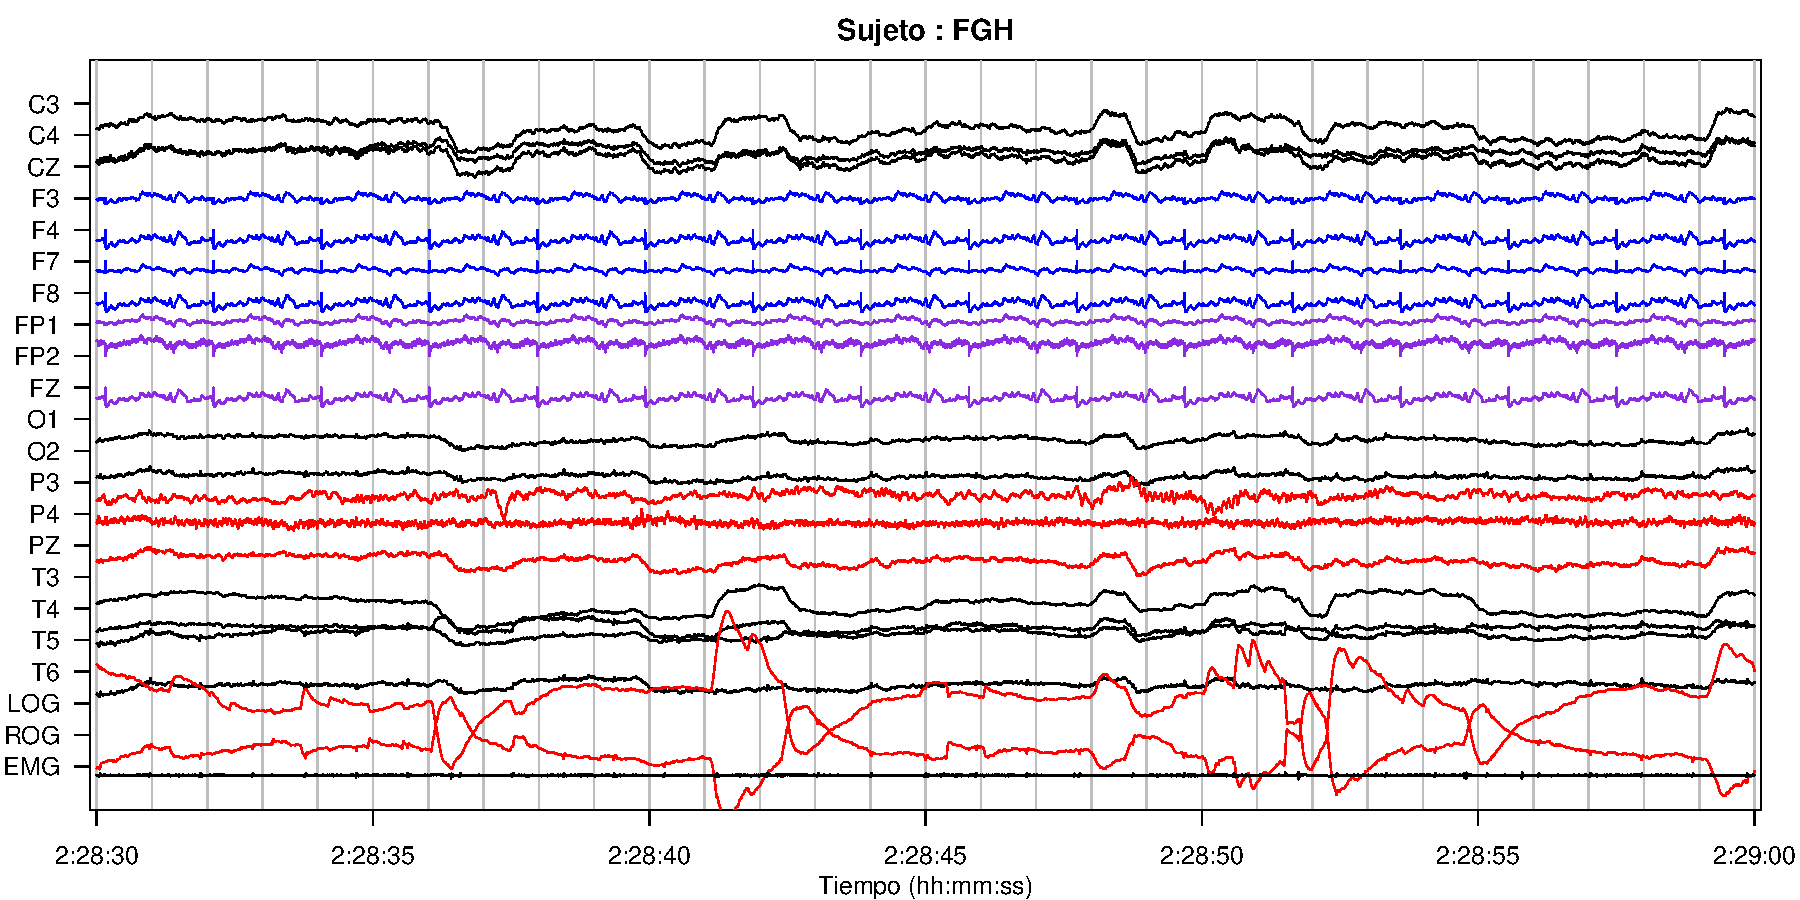
\includegraphics[width=0.95\linewidth]
{./img_ejemplos/FGH_297_PDG_lucirse_PSG.pdf} 
\caption{Una \'epoca t\'ipica del registro PSG para el sujeto FGH durante sue\~no MOR. N\'otense 
los patrones peri\'odicos en los canales correspondientes a la regi\'on frontal, que no 
corresponden a la actividad cerebral usual.}
\label{FGH_psg}
\end{figure}

\begin{figure}
\centering
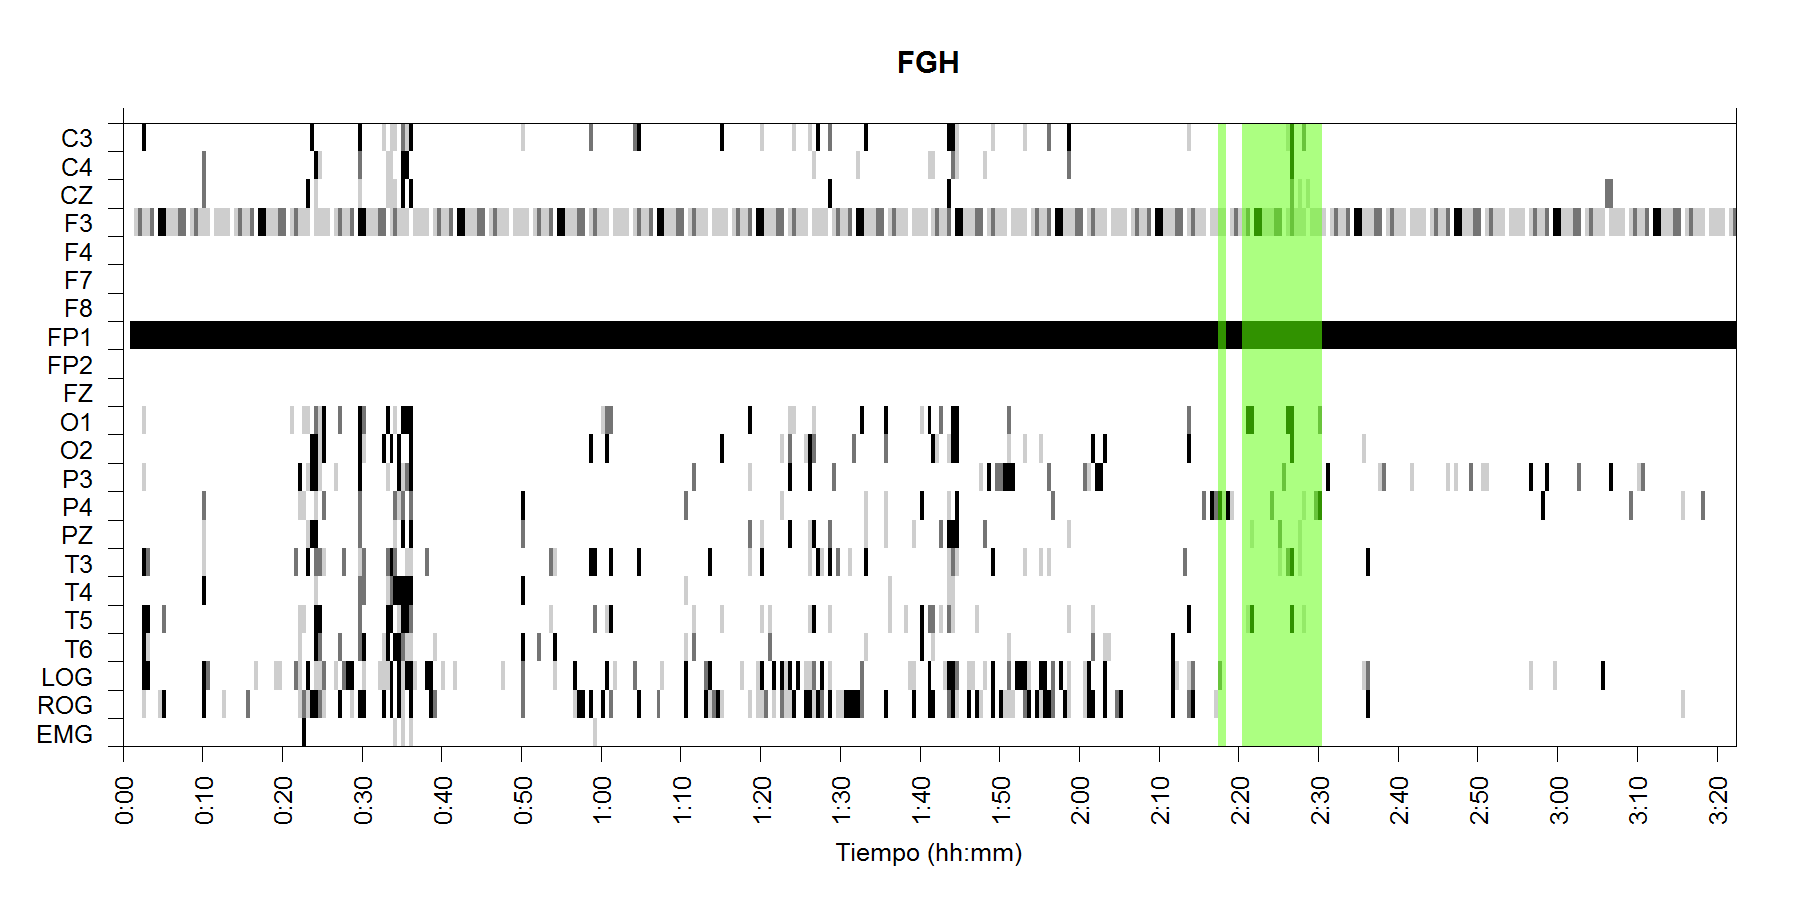
\includegraphics[width=0.95\linewidth]
{./img_ejemplos/FGHSUE_est.png} 
\caption{Compilado gr\'afico para el sujeto FGH; n\'otese el patr\'on inusual (completamente 
blanco o negro) en los canales correspondientes a la regi\'on frontal}
\label{FGH_especial}
\end{figure}

%%%%%%%%%%%%%%%%%%%%%%%%%%%%%%%%%%%%%%%%%%%%%%%%%%%%%%%%%%%%%%%%%%%%%%%%%%%%%%%%%%%%%%%%%%%%%%%%%%%
%%%%%%%%%%%%%%%%%%%%%%%%%%%%%%%%%%%%%%%%%%%%%%%%%%%%%%%%%%%%%%%%%%%%%%%%%%%%%%%%%%%%%%%%%%%%%%%%%%%

\subsection{Efecto del tama\~no de las \'epoca}

El uso de \'epocas de 30 segundos est\'a motivado por las recomendaciones de la AASM para 
clasificar, de manera estandarizada, las etapas de sue\~no a partir de registros de PSG 
\cite{AASM07}. 
No se discutir\'an en este trabajo motivaciones o evidencia para usar esta longitud de \'epoca en 
particular, ni para el caso contrario, sino que se acepta por fines de comparabilidad. 
Sin embargo, en alg\'un momento de este trabajo se usaron los registros de PSG organizados en 
\'epocas de 10 segundos de duraci\'on, como se muestra en la figura \ref{epocas_diferentes}. 
Se realizaron todos los an\'alisis descritos usando esta segmentaci\'on mixta (algunos sujetos con 
\'epocas de 10 s, otros con \'epocas de 30 s) y se obtuvieron resultados seg\'un los cuales no hay 
diferencias significativas en ninguno de los an\'alisis. 
Por otro lado, la representaci\'on gr\'afica construida a partir de los mismos datos, organizados
en \'epocas de 10 s, cambia sustancialmente (ver figura \ref{comp_VCR}).

\begin{figure}
\centering
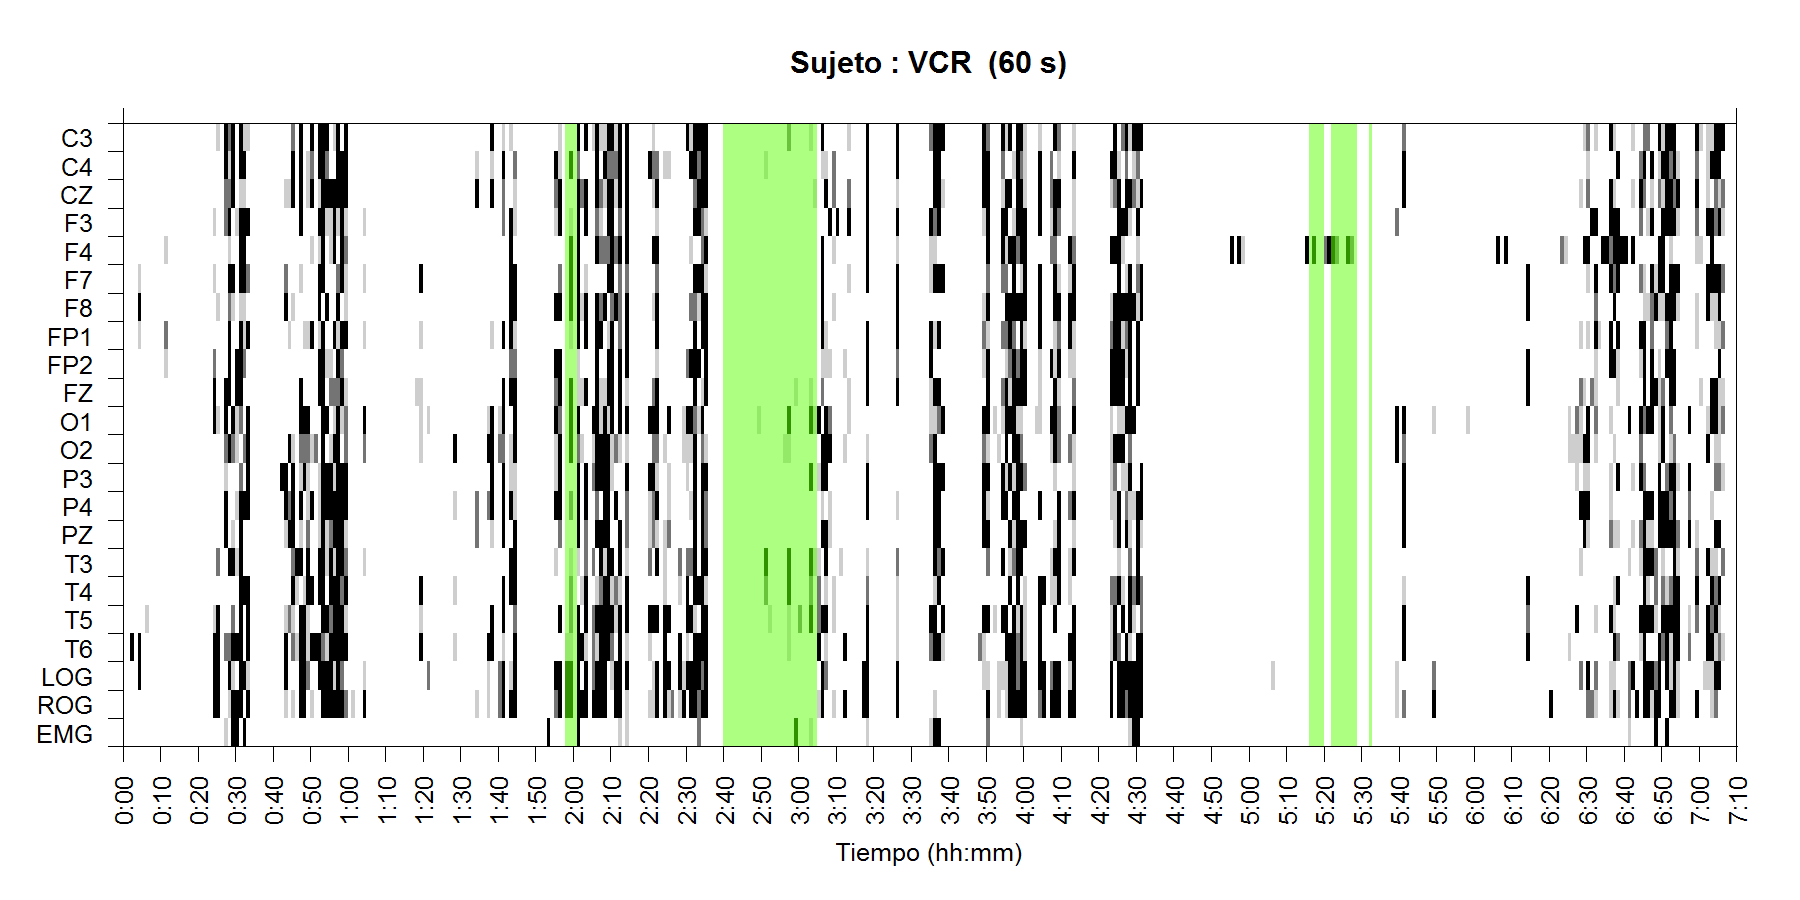
\includegraphics[width=0.9\linewidth] 
{./img_ejemplos/VCNNS1_est_60.png} 
\\
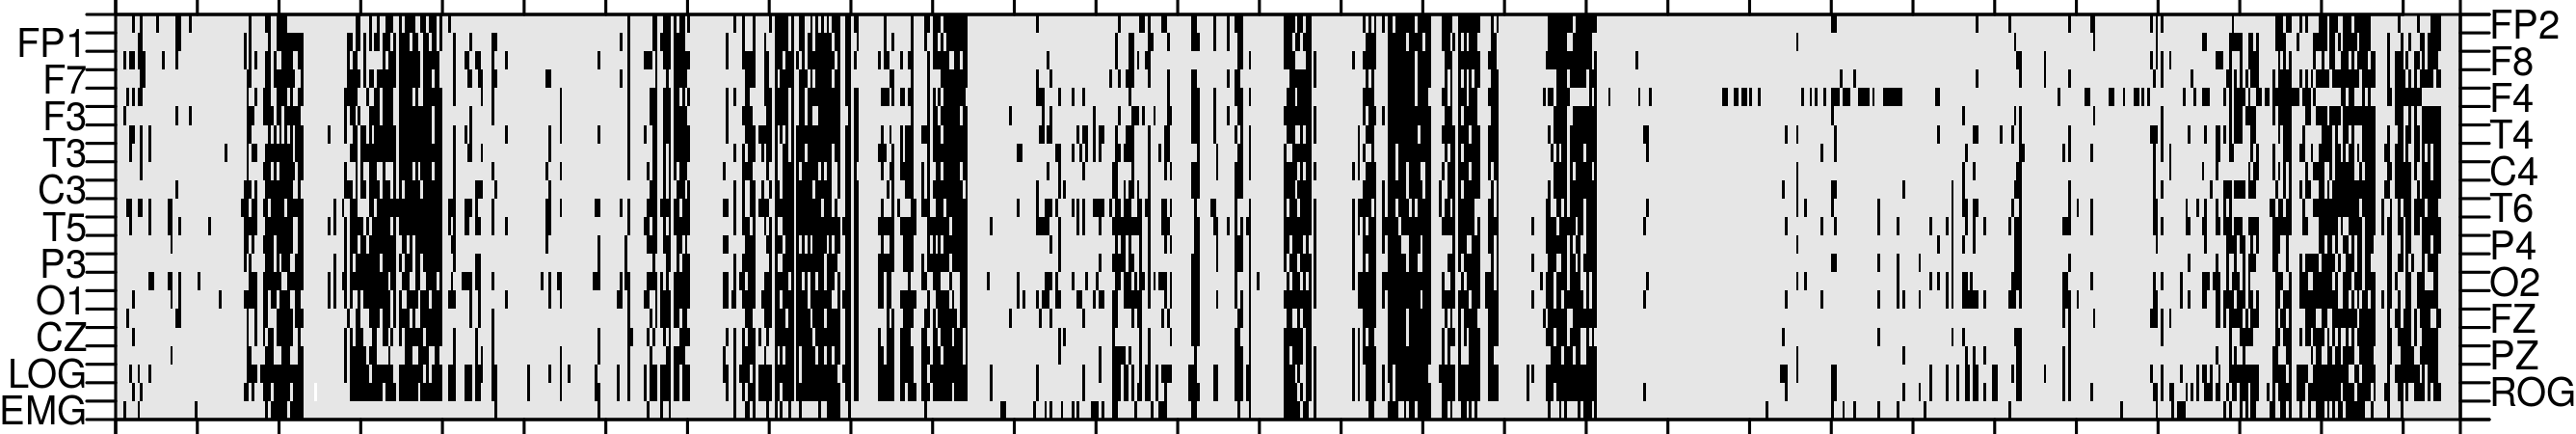
\includegraphics[width=0.9\linewidth]
{./img_ejemplos/VCNNS1_est_30.png} 
\\
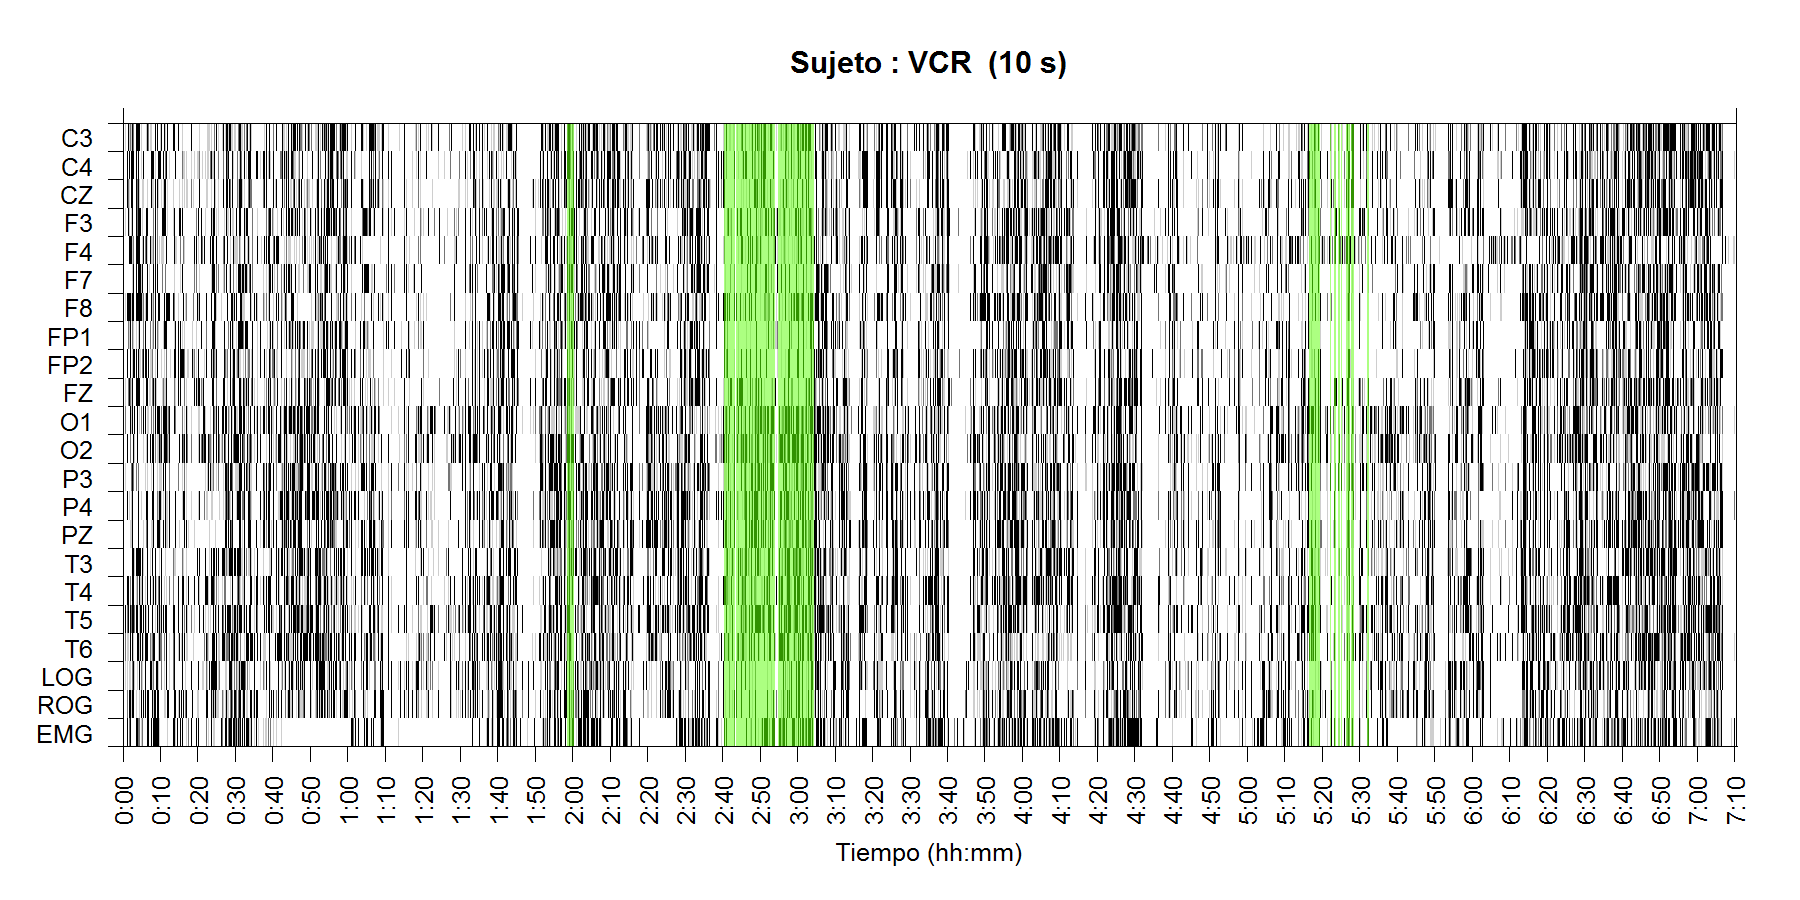
\includegraphics[width=0.9\linewidth]
{./img_ejemplos/VCNNS1_est_10.png} 
\caption{Compilaci\'on gr\'afica de las \'epocas clasificadas como PE, distribuidas en el tiempo
para cada uno de los canales. El registro corresponde al sujeto VCR, organizando el registro en
\'epocas de diferente duraci\'on}
\label{comp_VCR}
\end{figure}

El hecho de que los resultados fueran afectados de manera contundente por la forma en que se 
organizan los datos, sugiere que ser\'a provechoso prestar mayor atenci\'on a la naturaleza de las 
caracter\'isticas estudiadas y su posible interpretaci\'on en la fisiolog\'ia.
Se propone que los registros de PSG tienen una propiedad referida como 'estacionariedad local',
concepto introducido por Dahlhaus \cite{Dahlhaus97}.
A grosso modo, un proceso localmente estacionario es aqu\'el cuya FDE (que puede depender del 
tiempo) puede ser aproximada 'a trozos': usando FDE's correspondientes a procesos que poseen una 
representaci\'on espectral de Cram\'er y que est\'an 'correctamente ensamblados'.

%\begin{defn}[Estacionariedad local]
%Una secuencia de procesos estoc\'asticos de media cero, $\{ X_{t,N} \}$ con $t = 1, 2, \dots, N$, 
%se dicen localmente estacionarios en el tiempo $t_0 \in [0,1]$ si existe una representaci\'on del 
%tipo
%\begin{equation*}
%X_{t,N} = \intPI \widetilde{A_{t,N}}(\omega) e^{i \omega t} dZ(\omega)
%\end{equation*}
%donde se satisface que:
%\begin{itemize}
%\item $\{ Z(\omega) \}$ es un proceso de media cero con incrementos ortogonales, es decir
%\begin{equation*}
%\Cov{dZ(\omega_1),dZ(\omega_2)} =
%\begin{cases}
%d\omega &\text{, } \omega_1 = \omega_1 \\
%0 &\text{, otro caso}
%\end{cases}
%\end{equation*}
%\item Existe una constante $K$ y una funci\'on suave 
%$A: [0,1]\times [-\pi,\pi] \rightarrow \mathbb{C}$, 
%con $A(t_0,\omega) = \overline{A(t_0,-\omega)}$, tal que para toda $N$
%\begin{equation*}
%\sup_{\nicefrac{t}{N}\in \varepsilon_N(t_0)} 
%\sup_{\omega} \abso{ \widetilde{A_{t,N}}(\omega) - A(t_0,\omega) }
%\leq \frac{K}{N}
%\end{equation*}
%con $\varepsilon_N(t_0)$ es una vecindad de $t_0$ 
%tal que $\abso{\abso{\nicefrac{t}{N}-t_0}} = O(N^{-\alpha})$,
%%cuyo tama\~no es del orden $O(N^{-\alpha})$,
%con $0\leq \alpha < 1$
%\item $A(t_0,\omega)$ es continuo en $\{ t_0 \} \times [-\pi,\pi]$
%\end{itemize}
%\label{est_local}
%\end{defn}

Se propone que los registros de PSG se comportan como procesos localmente estacionarios; m\'as 
a\'un, esta caracter\'istica podr\'ia cambiar en adultos mayores con y sin PDC. 
Una motivaci\'on fisiol\'ogica para la hip\'otesis anterior es el contenido de los registros de
PSG: un conjunto descoordinado y homog\'eneo de ondas cerebrales, complejos K y husos de sue\~no.
Si bien esta composici\'on sugiere que la no-estacionariedad es la opci\'on m\'as obvia, el
an\'alisis llevado a cabo revela que el contenido de estos eventos no es homog\'eneo durante el
sue\~no; m\'as a\'un, mientras m\'as peque\~no sea el intervalo de tiempo observado, es m\'as
posible encontrar zonas de composici\'on m\'as o menos homog\'enea que puedan ser clasificadas
como PE.
Esta hip\'otesis explicar\'ia el cambio observado al cambiar el tama\~no de la \'epoca; de manera
arriesgada, se podr\'ia concluir que, entre los individuos con PDC, la homogeneidad del PSG es muy
similar durante MOR y NMOR.

%%%%%%%%%%%%%%%%%%%%%%%%%%%%%%%%%%%%%%%%%%%%%%%%%%%%%%%%%%%%%%%%%%%%%%%%%%%%%%%%%%%%%%%%%%%%%%%%%%%
%%%%%%%%%%%%%%%%%%%%%%%%%%%%%%%%%%%%%%%%%%%%%%%%%%%%%%%%%%%%%%%%%%%%%%%%%%%%%%%%%%%%%%%%%%%%%%%%%%%

\section{Conclusiones}

En registros de PSG para adultos mayores, segmentado en \'epocas de 30 segundos, la presencia 
proporcional de estacionariedad d\'ebil es significativamente diferente durante el sue\~no MOR y 
NMOR.
Estas diferencia se pudieron observar en el grupo Control para los canales C3, C4, F7, F8, FP1, 
FP2, O2, P4, LOG, ROG; en el grupo con PDC s\'olo se detectaron estas diferencias para los canales 
LOG y ROG.
Estos cambios entre MOR y NMOR pueden explicarse 
\begin{enumerate}
\item en LOG y ROG por las caracter\'isticas propias  del sue\~no MOR
\item en el resto de los canales (para el grupo Control), porque se tratan de la 
regi\'on frontal, asociada a la toma de decisiones, as\'i como la regi\'on posterior, 
asociada con la integraci\'on
de informaci\'on
\end{enumerate}

El an\'alisis de estacionariedad sobre registros de PSG para un adulto mayor con par\'alisis facial 
fue capaz de se\~nalar este padecimiento, visto como una ausencia total de \'epocas estacionarias
en una regi\'on concreta.

Los resultados encontrados sugieren que es posible interpretar los cambios neurofisiol\'ogicos 
durante el deterioro cognitivo como un cambio en la estructura funcional del cerebro al transitar 
entre sue\~no MOR y NMOR: el cambio es menos acentuado durante el PDC, pues tienen proporciones 
estad\'isticamente similares de \'epocas clasificadas como PE.
Esta interpretaci\'on propuesta es consistente con \cite{Valeria}.

En otro \'ambito, los patrones visuales descritos, visibles al mostrar gr\'aficamente la 
distribuci\'on de \'epocas PE, predicen parcialmente con las \'epocas de sue\~no MOR clasificadas 
por un experto (cuando menos en el grupo Control).
Se propone que la representaci\'on gr\'afica pudiera ser usado como auxiliar en la clasificaci\'on 
de segmentos de registro seg\'un la etapa de sue\~no.

Se presenta evidencia seg\'un la cual los registros de PSG, al menos para adultos mayores, no 
corresponden a series de tiempo no-estacionarias sino a series localmente estacionarias; esta 
distinci\'on cobra importancia al momento de elegir el tama\~no de ventana (en el tiempo) usada 
para organizar los registros.

%%%%%%%%%%%%%%%%%%%%%%%%%%%%%%%%%%%%%%%%%%%%%%%%%%%%%%%%%%%%%%%%%%%%%%%%%%%%%%%%%%%%%%%%%%%%%%%%%%%
%%%%%%%%%%%%%%%%%%%%%%%%%%%%%%%%%%%%%%%%%%%%%%%%%%%%%%%%%%%%%%%%%%%%%%%%%%%%%%%%%%%%%%%%%%%%%%%%%%%

\section{Trabajo a futuro}

Los resultados principales de este trabajo, con vista al trabajo futuro, consiste en las 
diferencias encontradas entre el sue\~no MOR y NMOR, as\'i como los patrones visuales asociados con 
la aparici\'on de sue\~no MOR; tales caracter\'isticas s\'olo fueron presentes para el grupo 
Control. Si bien no constituyen propiamente marcadores de deterioro cognitivo, esta metodolog\'ia
podr\'ia extenderse para identificar tales marcadores.
Por ejemplo, un marcador conocido \cite{Becerra12} del deterioro cognitivo es el 'enlentecimiento' 
de la actividad cerebral, entendido como un cambio en la concentraci\'on de energ\'ia desde ondas 
r\'apidas a ondas lentas.
Para detectar la estacionariedad d\'ebil se ha usado prueba de Priestley-Subba Rao, basada en 
estimadores locales para la funci\'on de densidad espectral (FDE); estos mismos estimadores 
podr\'ian ser usados para corroborar si efectivamente existen diferencias en la FDE para registros 
de adultos mayores con y sin deterioro cognitivo. 

Finalmente, y como se mencion\'o anteriormente, los patrones visuales en la representaci\'on 
gr\'afica pueden tener un uso como caracter\'isticas auxiliares para la detecci\'on 
semi-autom\'atica de \'epocas MOR en registros de PSG; en ese sentido, cabe mencionar el caso de 
los sujetos excluidos del estudio, para los cuales estos patrones parecen no cumplirse. 
Es en principio posible que la identificabilidad del sue\~no MOR, a trav\'es de estos patrones, 
pudiera fungir como marcador cl\'inico.

%%%%%%%%%%%%%%%%%%%%%%%%%%%%%%%%%%%%%%%%%%%%%%%%%%%%%%%%%%%%%%%%%%%%%%%%%%%%%%%%%%%%%%%%%%%%%%%%%%%
%%%%%%%%%%%%%%%%%%%%%%%%%%%%%%%%%%%%%%%%%%%%%%%%%%%%%%%%%%%%%%%%%%%%%%%%%%%%%%%%%%%%%%%%%%%%%%%%%%%
%%%%%%%%%%%%%%%%%%%%%%%%%%%%%%%%%%%%%%%%%%%%%%%%%%%%%%%%%%%%%%%%%%%%%%%%%%%%%%%%%%%%%%%%%%%%%%%%%%%
%%%%%%%%%%%%%%%%%%%%%%%%%%%%%%%%%%%%%%%%%%%%%%%%%%%%%%%%%%%%%%%%%%%%%%%%%%%%%%%%%%%%%%%%%%%%%%%%%%%


\appendix

%%%%%%%%%%%%%%%%%%%%%%%%%%%%%%%%%%%%%%%%%%%%%%%%%%%%%%%%%%%%%%%%%%%%%%%%%%%%%%%%%%%%%%%%%%%%%%%%%%%%
%%%%%%%%%%%%%%%%%%%%%%%%%%%%%%%%%%%%%%%%%%%%%%%%%%%%%%%%%%%%%%%%%%%%%%%%%%%%%%%%%%%%%%%%%%%%%%%%%%%
%%%%%%%%%%%%%%%%%%%%%%%%%%%%%%%%%%%%%%%%%%%%%%%%%%%%%%%%%%%%%%%%%%%%%%%%%%%%%%%%%%%%%%%%%%%%%%%%%%%
%%%%%%%%%%%%%%%%%%%%%%%%%%%%%%%%%%%%%%%%%%%%%%%%%%%%%%%%%%%%%%%%%%%%%%%%%%%%%%%%%%%%%%%%%%%%%%%%%%%
\chapter{Detalles}

Se exponen varios de los conceptos expuestos como preeliminares pero con las formalidades
pertinentes; cabe mencionar que todos estos resultados no son originales del presente trabajo,
razón por la cual fueron omitidos anteriormente.
%presentados como preeliminares, incluyendo demostraciones. 
%Esta informaci\'on fue cortada del 
%cuerpo principal del trabajo porque no son resultados originales, y si bien son sumamaente
%importantess e interesantes, se omitieron a favor de los resultados originales generados en el 
%trabajo.

%%%%%%%%%%%%%%%%%%%%%%%%%%%%%%%%%%%%%%%%%%%%%%%%%%%%%%%%%%%%%%%%%%%%%%%%%%%%%%%%%%%%%%%%%%%%%%%%%%%
%%%%%%%%%%%%%%%%%%%%%%%%%%%%%%%%%%%%%%%%%%%%%%%%%%%%%%%%%%%%%%%%%%%%%%%%%%%%%%%%%%%%%%%%%%%%%%%%%%%

\section{Variable aleatoria}

Un primer motivo para esta sección es enfatizar que, formalmente, una variable aleatoria se concibe 
como un espacio de medida y no como un recuento de eventos. 
Paralelamente, introducir la terminología adecuada permitirá entender los teoremas que dan base
a los análisis realizados.
%relevante para varios resultados utilizados, por lo que
%conviene no omitirla.
%
%Antes de poder definir formalmente las variable aleatoria, debe definirse las medidas.

\begin{defn}[$\boldsymbol{\sigma}$-álgebra]
Sea $U$ un conjunto y $\mathcal{U}$ una colección de subconjuntos de $U$. Se dice que $\mathcal{U}$
es una $\sigma$-álgebra si comple que
\begin{itemize}
\item $U \in \mathcal{U}$
\item $A \in \mathcal{U}$ implica que $A^{C} \in \mathcal{U}$
\item Si $\{ A_n \}_{n\in \mathbb{N}}$ son conjuntos tales que $A_i \in \mathcal{U}$, entonces
$\displaystyle \cup_{n\in \mathbb{N}} A_n \in \mathcal{U}$
\end{itemize}
Donde $A^{C}$ es el complemento $\{ u \in U | u \notin A \} $
\end{defn}

Por simplicidad, en este trabajo sólo se usarán medidas para conjuntos de números reales derivadas 
de la $\sigma$-álgebra de Borel, que es definida como la $\sigma$-álgebra más pequeña que contiene a 
los intervalos abiertos abiertos\footnote{Si una $\sigma$-álgebra contiene a todos los
intervalos abiertos, entonces debe contener a todos los elementos de la $\sigma$-álgebra de Borel}.

\begin{defn}[Medida]
Sea $U$ un conjunto y $\mathcal{U}$ una $\sigma$-álgebra definida en $U$. Se dice que una función
$\mu : \mathcal{U} \rightarrow \R \cup {\infty}$ es una medida si cumple que
\begin{itemize}
\item $\mu(\emptyset) = 0$
\item $\mu(A) \geq 0$ para cualquier $A \in \mathcal{U}$
\item Si $\{ A_n \}_{n\in \mathbb{N}}$ son conjuntos disjuntos a pares y tales que 
$A_i \in \mathcal{U}$, entonces 
$\displaystyle \mu\left( \cup_{n\in \mathbb{N}} A_n \right) = \sum_{n\in \mathbb{N}} \mu(A_n)$
\end{itemize}
Donde $\emptyset$ es el conjunto vacío %y $\R^{*} = \R \cup \{-\infty,\infty \}$
\end{defn}

\begin{defn}[Medida de probabilidad en $\boldsymbol{\R}$]
Sea $\mathcal{B}$ la sigma álgebra de Borel definida para $\R$, se dice que una función
$P : \mathcal{B} \rightarrow [0.1]$ es una \textbf{medida de probabilidad} si cumple que
\begin{itemize}
\item $P(\emptyset) = 0$
\item $0 \leq P(A) \leq 1$ para cualquier $A \in \mathcal{B}$
\item Si $A, B \in \mathcal{B}$ y $A\cap B = \emptyset$, entonces $P(A \cup B) = P(A) + P(B)$ 
\item $P(\R) = 1$
\end{itemize}
\label{variable_aleatoria}
\end{defn}

%Cabe mencionar que cuando se usa una variable aleatoria para modelar un fenómeno, existe un paso
%intermedio en que los eventos relevantes se asocian con números reales

Otra forma de entender una variables aleatoria es a partir de su función de probabilidad
acumulada (FPA), ya que hay una correspondencia unívoca entre cada variable aleatoria y su FPA.

\begin{defn}[Función de Probabilidad Acumulada]
Sea 
\begin{equation*}
F_X (x) = P\left( (-\infty,x] \right)
\end{equation*}
\end{defn}

Habitualmente, como se hace el presente texto, se usa el símbolo $X$ para denotar a una variable 
aleatoria cuya FDA es $F_X$; bajo esta idea, para cualquier conjunto $I \subseteq \R$ se denota
$P(X \in I) = P(I)$

%%%%%%%%%%%%%%%%%%%%%%%%%%%%%%%%%%%%%%%%%%%%%%%%%%%%%%%%%%%%%%%%%%%%%%%%%%%%%%%%%%%%%%%%%%%%%%%%%%%
%%%%%%%%%%%%%%%%%%%%%%%%%%%%%%%%%%%%%%%%%%%%%%%%%%%%%%%%%%%%%%%%%%%%%%%%%%%%%%%%%%%%%%%%%%%%%%%%%%%

\section{Notas sobre la estacionariedad}

En el texto se presentó la estacionariedad débil (definición \ref{est_usual}) como la característica
a verificar en los registros de estudio, aunque cabe ahondar un poco sobre por qué
la versión \textit{débil}. La estacionariedad formaliza el que
las características de un proceso estocástico no cambien en el tiempo, lo cual permite 
caracterizarlo a partir de sus realizaciones; la definición \ref{est_fuerte} presenta
una condición suficiente para ello.

\begin{defn}[Estacionariedad fuerte]
Un proceso estoc\'astico \xt es fuertemente estacionario si, para cualquier conjunto de 
tiempos admisibles
$t_1,t_2,\dots,t_n$ y cualquier $\tau$ tal que los tiempos $t_i+\tau$ son admisibles; se cumple que
\begin{equation*}
F_{\left(X(t_1),X(t_2),\dots,X(t_n)\right) }
\equiv
F_{\left(X(t_1+\tau),X(t_2+\tau),\dots,X(t_n+\tau)\right)}
\end{equation*}

Donde $F_{\left(X(t_1),X(t_2),\dots,X(t_n)\right) }$ es la funci\'on de probabilidad acumulada 
conjunta para el vector $\left(X(t_1),X(t_2),\dots,X(t_n)\right)$
\label{est_fuerte}
\end{defn}

Tal definición es problemática en el problema tratado, ya que requiere estimar para cada tiempo

%Sin embargo, la definici\'on \ref{est_fuerte} resulta in\'util si se pretende verificar que un 
%registro dado pudiera ser modelado como la realizaci\'on de un proceso es fuertemente estacionario 
%(un objetivo descartado para este trabajo). 
%En ese escenario, para cada tiempo registrado $t$ se 
%tiene s\'olo una observaci\'on para cada variable aleatoria $X(t)$, lo cual es muy poca 
%informaci\'on como para estimar las funciones de probabilidad acumulada mencionadas en la 
%definici\'on.
%Estas limitaciones motivan una definici\'on m\'as d\'ebil de estacionariedad, pero que pueda ser 
%detectada en realizaciones dadas de procesos; se exhibe la definici\'on \ref{est_orden_m} como 
%alternativa.

\begin{defn}[Estacionariedad de orden $\boldsymbol{m}$]
Un proceso estoc\'astico $\{ X(t) \}$ se dice estacionario de orden $m$ si, para cualquier conjunto 
de tiempos admisibles $t_1,t_2,\dots,t_n$ y cualquier $\tau \in \R$ se cumple que
\begin{equation*}
\E{ X^{m_1}(t_1)X^{m_2}(t_2)\cdots X^{m_n}(t_n) }
=
\E{ X^{m_1}(t_1+\tau)X^{m_2}(t_2+\tau)\cdots X^{m_n}(t_n+\tau) }
\end{equation*}
Para cualesquiera enteros $m_1,m_2,\dots,m_n$ tales que $m_1+m_2+\dots+m_n \leq m$
\label{est_orden_m}
\end{defn}

Para entender mejor la definici\'on \ref{est_orden_m} y sus limitaciones frente a la 
estacionariedad fuerte, consid\'erense tres procesos: $\{X(t)\}$ fuertemente estacionario, 
$\{Y_1(t)\}$ estacionario de orden 1, y $\{Y_2(t)\}$ estacionario de orden 2. Luego
\begin{itemize}
\item Las medias\footnote{La media de una variable aleatoria $V$ se define como $ \mu_V := \E{V}$} 
$ \mu_{X(t)}$, $ \mu_{Y_1(t)}$ y $ \mu_{Y_2(t)}$ no dependen de $t$

\item Las varianzas\footnote{La varianza de una variable aleatoria $V$ se define como 
$ \Var{V} := \E{\left(V - \mu_V \right)^{2}}$} $ \Var{Y_1(t)}$ y $ \Var{Y_2(t)}$ no dependen de 
$t$, pero no se puede garantizar lo mismo para $\Var{X(t)}$

\item El coeficiente de asimetr\'ia\footnote{El coeficiente de asimetr\'ia para una variable 
aleatoria $V$ se define como 
$\gamma_V = \frac{\E{\left(V-\mu_V\right)^{3}}}{\Var{V}^{\nicefrac{3}{2}}}$}
$ \gamma_{X(t)}$ no depende de $t$, pero no se puede garantizar lo mismo para $ \gamma_{Y_1(t)}$ ni 
para $ \gamma_{Y_2(t)}$
\end{itemize}

Cabe mencionar que hay una relaci\'on de contenci\'on clara en familia de los conjuntos de procesos 
estacionarios de orden finito (si un proceso es estacionario de orden $m$, entonces es estacionario 
de orden $n$ para todo $n \leq m$); es posible definir procesos estacionarios de orden 'infinito' 
seg\'un \ref{est_orden_m}, que intuitivamente ser\'ian fuertemente estacionarios. 
De manera pragm\'atica, en este trabajo no se discuten tales interrogantes, sino que se usar\'a 
\'unicamente la definici\'on correspondiente al caso $m=2$, referida como estacionariedad d\'ebil o 
de orden 2, y repetida en la definici\'on \ref{est_orden_2}.



\begin{defn}[Estacionariedad d\'ebil]
Un proceso estoc\'astico \xt es d\'ebilmente estacionario si, para cualesquiera tiempos 
admisibles\footnote{El t\'ermino \textit{tiempos admisibles} indica que para tiempo 
discreto o continuo la afirmaci\'on es la misma, bajo las restricciones pertinentes} 
$t, s, t+\tau, s+\tau$, se cumple que
\begin{center}
\begin{tabular}{ccc}
$\E{X(t)} = \E{X(t+\tau)}$
& y &
$\E{X(t)X(s)} = \E{X(t+\tau)X(s+\tau)}$
\end{tabular}
\end{center}
\label{est_orden_2}
\end{defn}

M\'as a\'un, parece conveniente exhibir una caracterizaci\'on equivalente para los procesos 
d\'ebilmente estacionarios, pero que tiene una interpretaci\'on m\'as sencilla.
\begin{thrm}
Un proceso estoc\'astico es d\'ebilmente estacionario si y s\'olo si para cualesquiera tiempos 
admisibles $t$, $s$ se tiene que
\begin{itemize}
\item $\E{X(t)} = \mu_X$
\item $\Var{X(t)} = \sigma^{2}_X$
\item $\Cov{X(t),X(s)} = \rho_X (s-t)$
\end{itemize}
Donde $\mu_X$, $\sigma^{2}_X$ son constantes, $\rho_X(\tau)$ es una funci\'on que \'unicamente 
depende de $\tau$
\label{est_usual}
\end{thrm}

-----------------

Cabe comentar  sobre la existencia de procesos que son fuertemente estacionarios pero que no son 
estacionarios de ning\'un orden: por ejemplo, un proceso de variables aleatorias independientes con 
distribuci\'on de Cauchy\footnote{Una variable aleatoria tiene distribuci\'on de Cauchy si su 
funci\'on de probabilidad acumulada es de la forma 
$\displaystyle F(x) = \frac{1}{\pi} \int_{-\infty}^{x} \frac{1}{1+y^{2}} dy$}.
Una condici\'on suficiente para que un proceso fuertemente estacionario sea estacionario de orden 
$m$ es que tenga sus primeros $m$ momentos bien definidos.
Con respecto a las se\~nales registradas en el EEG, entendidas como procesos estoc\'asticos, se 
espera que tengan (cuando menos) segundos momentos bien definidos; m\'as adelante se presentan 
argumentos, desde una interpretaci\'on f\'isica, sobre por qu\'e se espera que ocurra lo anterior.



-------------------

Como ejemplos, un proceso ruido blanco (definici\'on \ref{r_blanco}) no es estoc\'asticamente 
continuo, mientras que un proceso de Wiener (definici\'on \ref{r_wiener}) s\'i lo es.

\begin{defn}[Proceso ruido blanco]
Se dice de un proceso estoc\'astico $\{ R(t) \}$ que cumple, para cualesquiera tiempos admisibles
$t$ y $s$, las siguientes propiedades:
\begin{itemize}
\item $\E{R(t)}=0$
\item $\Cov{R(t),R(s)}=0 \Leftrightarrow t=s$ 
\end{itemize}
\label{r_blanco}
\end{defn}

\begin{defn}[Proceso de Wiener]
Se dice de un proceso estoc\'astico $\{ W(t) \}$ que cumple, para cualesquiera tiempos admisibles
$t$ y $s$ (con $s>t$) las siguientes propiedades:
\begin{itemize}
\item $W(0) = 0$ ($W(0)$ es constante)
\item $W(s)-W(t)$ es independiente de $W(u)$, para todo $u<t$ admisible
\item $W(s)-W(t) \sim N(0,\abso{t-s})$  (los incrementos tienen distribuci\'on normal)
\end{itemize}
\label{r_wiener}
\end{defn}

Una forma natural de pensar en la definici\'on \ref{cont_est} es que, si $\abso{t-t_0}$ es muy 
peque\~no, entonces $X(t)$ y $X(t_0)$ difieren muy poco entre s\'i (como variables aleatorias).
Es destacable que si un proceso es estoc\'asticamente continuo en un intervalo, sus realizaciones 
solamente se pueden garantizar continuas casi en todas partes \footnote{Una propiedad se cumple 
\textbf{casi en todas partes} si se cumple en un conjunto cuyo complemento tiene medida cero} en 
ese intervalo.

--------------------------

En la definici\'on \ref{fourier_stieltjes}, si $F$ es derivable en todas partes entonces $F\prima$ 
cumple el mismo papel que la integral de Fourier; en cambio, si $k$ es una funci\'on peri\'odica 
entonces $F$ toma una forma escalonada cuyos aumentos coinciden con la serie de Fourier para $k$. 
M\'as a\'un, existen funciones que no son ni peri\'odicas ni absolutamente sumables pero poseen 
una transformada de Fourier-Stieltjes, como $k(x)=\SEN{x}+\SEN{\sqrt{2}x}$, 
$k(x)=\COS{x} + (1+x^{2})^{-1}$.

%\begin{comment}
\begin{thrm}[Descomposici\'on de Lebesgue]
Sea $f:I\rightarrow \R$ una funci\'on de variaci\'on acotada, con $I$ un intervalo. Entonces pueden 
hallarse funciones $f_j, f_c, f_a :I\rightarrow \R$ tales que
\begin{itemize}
\item $f = f_j+ f_c+ f_a$
\item $f_j = \sum_{y \leq x} f(x-0) + f(x+0)$
\item $f_a$ es absolutamente continua\footnote{Para que una funci\'on sea absolutamente continua,
basta que sea de variaci\'on acotada y que mapee conjuntos de medida cero en conjuntos de medida
cero} en $I$
\item $f_c$ es una funci\'on singular\footnote{Una funci\'on es singular si es continua, de 
variaci\'on acotada y no-constante, y se cumple que tiene derivada cero casi en todas partes} en 
$I$
\end{itemize}
Estas funciones son \'unicas excepto por constantes, y en conjunto son llamados la 
\textit{descomposici\'on de Lebesgue} de $f$
\label{Lebesgue_decomp}
\end{thrm}
%\end{comment}

%%%%%%%%%%%%%%%%%%%%%%%%%%%%%%%%%%%%%%%%%%%%%%%%%%%%%%%%%%%%%%%%%%%%%%%%%%%%%%%%%%%%%%%%%%%%%%%%%%%
%%%%%%%%%%%%%%%%%%%%%%%%%%%%%%%%%%%%%%%%%%%%%%%%%%%%%%%%%%%%%%%%%%%%%%%%%%%%%%%%%%%%%%%%%%%%%%%%%%%

\section{Transformada R\'apida de Fourier}

Como se mostró en el texto, la transformada de Fourier es un operador clave para la definición y el
estudio del \textit{dominio de las frecuencias}. Sin embargo, su aplicación a series de tiempo grandes se ve
dificultada porque es un proceso lento: si se toma una serie de tiempo 
$\{s_n\}_{n=0,\dots,N}$ y se calcula su transformada finita de Fourier según su definición
\begin{equation*}
\mathfrak{F}_s(\omega) = \sum_{n=0}^{N} s_n e^{i \omega n}
\end{equation*}
entonces para cada frecuencia $\omega$ se requerirán $N$ multiplicaciones y $N-1$ sumas, siendo que
usualmente se analizan las frecuencias de la forma $\omega_k = \nicefrac{2 \pi k}{N}$ 
con $k = 0, 1, \dots, \nicefrac{N}{2}$.
Usando la notación de Landau (definición \ref{orden}) se deduce que obtener la transformada discreta
de Fourier de una serie de tiempo de longitud $N$, usando este método, 
ocupa un tiempo de orden $\mathcal{O}(N^{2})$.

\begin{defn}[Orden $\mathcal{O}$]
Sean $f, g$ dos funciones en $\R$ con $g(x)\neq 0$ para $x\in \R$. Se dice que $f = \mathcal{O}(g)$,
que $f$ tiene orden $g$, si existe una constante $k\in \R$ tal que
\begin{equation*}
\lim_{x\rightarrow \infty} \frac{f(x)}{g(x)} = k
\end{equation*}
\label{orden}
\end{defn}

El algoritmo presentado por Cooley y Tukey en 1965, la Transformada Rápida de Fourier 
(TRF), usa menos operaciones si el número de observaciones es \textit{altamente 
compuesto}\footnote{Se dice que un número entero es \textit{compuesto} si no tiene dos o más
divisores propios mayores a 1; se dice que es más compuesto si tiene más de estos factores}.

Considerando la serie de tiempo $\{s_n\}_{n=0,\dots,N}$ con $N$ de la forma $N= p q$ para 
$p, q$ enteros mayores a 1, entonces su TRF se puede reescribir como

\begin{align*}
\mathfrak{F}_s(\omega) &= \sum_{m = 0}^{p} \sum_{k=0}^{q} s_n e^{i \omega (mp + q)} 
\\
&= 
\end{align*}

%%%%%%%%%%%%%%%%%%%%%%%%%%%%%%%%%%%%%%%%%%%%%%%%%%%%%%%%%%%%%%%%%%%%%%%%%%%%%%%%%%%%%%%%%%%%%%%%%%%
%%%%%%%%%%%%%%%%%%%%%%%%%%%%%%%%%%%%%%%%%%%%%%%%%%%%%%%%%%%%%%%%%%%%%%%%%%%%%%%%%%%%%%%%%%%%%%%%%%%

%\section{Efecto del filtro STL}
%
%En el texto se menciona al filtro STL como un algoritmo para eliminar los efectos de tendencias
%deterministas sobre los registros, con lo cual se puede argumentar que los registros tienen
%valor esperado cero y que admiten una representaci\'on de Wold-Cram\'er. Sin embargo, se omiti\'o
%una descripci\'on m\'as adecuada por motivos narrativos.
%
%El algoritmo, introducido por Cleveland y colaboradores en 1990 \cite{Cleveland1990} toma sus siglas
%del ingl\'es \textit{Seasonal-Trend decomposition based on Loess} (descomposici\'on en tendencia y
%periodicidad basada en loess)

%%%%%%%%%%%%%%%%%%%%%%%%%%%%%%%%%%%%%%%%%%%%%%%%%%%%%%%%%%%%%%%%%%%%%%%%%%%%%%%%%%%%%%%%%%%%%%%%%%%
%%%%%%%%%%%%%%%%%%%%%%%%%%%%%%%%%%%%%%%%%%%%%%%%%%%%%%%%%%%%%%%%%%%%%%%%%%%%%%%%%%%%%%%%%%%%%%%%%%%
%%%%%%%%%%%%%%%%%%%%%%%%%%%%%%%%%%%%%%%%%%%%%%%%%%%%%%%%%%%%%%%%%%%%%%%%%%%%%%%%%%%%%%%%%%%%%%%%%%%
%%%%%%%%%%%%%%%%%%%%%%%%%%%%%%%%%%%%%%%%%%%%%%%%%%%%%%%%%%%%%%%%%%%%%%%%%%%%%%%%%%%%%%%%%%%%%%%%%%%

%%%%%%%%%%%%%%%%%%%%%%%%%%%%%%%%%%%%%%%%%%%%%%%%%%%%%%%%%%%%%%%%%%%%%%%%%%%%%%%%%%%%%%%%%%%%%%%%%%%
%%%%%%%%%%%%%%%%%%%%%%%%%%%%%%%%%%%%%%%%%%%%%%%%%%%%%%%%%%%%%%%%%%%%%%%%%%%%%%%%%%%%%%%%%%%%%%%%%%%
%%%%%%%%%%%%%%%%%%%%%%%%%%%%%%%%%%%%%%%%%%%%%%%%%%%%%%%%%%%%%%%%%%%%%%%%%%%%%%%%%%%%%%%%%%%%%%%%%%%
%%%%%%%%%%%%%%%%%%%%%%%%%%%%%%%%%%%%%%%%%%%%%%%%%%%%%%%%%%%%%%%%%%%%%%%%%%%%%%%%%%%%%%%%%%%%%%%%%%%

\chapter{Ondas y frecuencias}

\section{Transformada de Fourier como operador}

La exposición inicia con los espacios de las \textbf{series $\boldsymbol{p}$-sumables}
($\lp$), y las  \textbf{funciones $\boldsymbol{p}$-integrables} sobre un intervalo 
$I \subseteq \R$ ($\llp$).
%; en el presente trabajo sólo se usarán los casos $p=1,2$.
%
%\begin{align}
%\ell^{p} &:= \left\{ s: \Z\rightarrow\C \talque \sum_{n=-\infty}^{\infty} \abso{s(n)}^{p} < \infty \right\}
%\label{lpdef} \\
%L^{p}[I] &:= \left\{ S: I\rightarrow\C \talque \int_I \abso{S(t)}^{p} dt < \infty \right\}
%\label{llpdef}
%\end{align}
\begin{align*}
\ell^{p} &:= \left\{ s: \Z\rightarrow\C \talque \sum_{n=-\infty}^{\infty} \abso{s(n)}^{p} < \infty \right\}
\\
L^{p}[I] &:= \left\{ S: I\rightarrow\C \talque \int_I \abso{S(t)}^{p} dt < \infty \right\}
\end{align*}

Estos espacios admiten las operaciones $+$, $\cdot$ y multiplicación por escalares complejos de la 
manera usual.%, es decir

%\begin{align*}
%s, z \in \lp, c \in \C \Rightarrow 
%[s+z](n) &= s(n) + z(n) \\
%[s\cdot z](n) &= s(n) z(n) \\
%[c \cdot s](n) &= s(n)c \\
%S, Z \in \llp, c \in \C \Rightarrow 
%[S+Z](t) &= S(t) + Z(t) \\
%[S\cdot Z](t) &= S(t)  Z(t) \\
%[c \cdot S](t) &= S(t)c
%\end{align*}
%
%En las próximas líneas se seguirán usando $s, z, S, Z, c$.

Para el caso particular $p=2$, los conjuntos $\ldos$ y $\lldos$ admiten los siguientes productos 
internos:
%
\begin{align*}
\left\langle s,z \right\rangle &= \sum_{n=-\infty}^{\infty} s(n) \overline{z(n)}\\
\left\langle S,Z \right\rangle &= \int_I S(t) \overline{Z(t)} dt
\end{align*}

Usando dichos productos internos, junto con las normas y métricas que inducen, los conjuntos 
$\ldos$ y $\lldos$ tienen estructura de \textbf{espacio de Hilbert}.

Con las definiciones anteriores, que muestran que $\ldos$ y $\lldos$ son \textit{muy}
parecidos, se puede formular unas definición para la transformada de Fourier como una equivalencia
entre estos espacios.

%{De manera pragm\'atica, en el presente trabajo la 
%palabra  'frecuencia' se usar\'a para referirse a la cantidad $q$ en expresiones del tipo 
%$e^{i q t}$}

\begin{definicion}[Serie de Fourier]
Sea $S: \R \rightarrow \C$ una función periódica con periodo $2T$ y tal que 
$S \in L^{2}\left[[-T,T]\right]$. Se dice que $A$ es la serie de Fourier para $S$ si cumple que
\begin{equation*}
A(n) = \frac{1}{2 T} \simint{T} S(t) e^{-\nicefrac{ i \abso{n} t}{2T}} dt
\end{equation*}
%Adicionalmente, la función $\mathcal{F} : \lldos \rightarrow \ldos : S \mapsto A$  recibe el nombre
%de \textbf{Transformada de Fourier}
\label{FourierClasico}
\end{definicion}

\begin{definicion}[Transformada de Fourier]
Sean $S$ y $A$ como en la definición \ref{FourierClasico}. Se le llama transformada de Fourier a la
función $\mathcal{F}_T : L^{2}\left[[-T,T]\right] \rightarrow \ldos : S \mapsto A$
\end{definicion}

Puede interpretarse a $A$ como las \textit{coordenadas} de $S$ en $L^{2}\left[[-T,T]\right]$, 
usando una base de funciones $\left\{ e^{\nicefrac{i \abso{n} t}{2 T}} \right\}_{n\in \Z}$, las
cuales resultan ser ortonormales; esta base en particular es conocida como la \textbf{base de 
Fourier}.
Se demuestra en el anexo A que $\mathcal{F_T}$ está bien definida en el sentido de 
tener efectivamente el dominio y codominio indicados. Así mismo, cabe mencionar las siguientes 
propiedades de $\mathcal{F}_T$
\begin{itemize}
\item Es lineal, es decir, $\mathcal{F}_T[cS + Z] = c\mathcal{F}_T[S] + \mathcal{F}_T[Z]$

\item \textbf{No} es invertible, aunque se le suele definir una
pseudoinversa\footnote{$\mathcal{F}_T^{\text{inv}}$ es \textit{exacta} salvo por la suma
de alguna función $S_0$ tal que $\int_{-T}^{T}\abso{S_0(t)}dt = 0$} como
\begin{equation*}
\mathcal{F}_{T}^{\text{inv}} : \ldos \rightarrow L^{2}\left[[-T,T]\right] :
A \mapsto \sum_{n -\infty}^{\infty} A(n) e^{\nicefrac{i \abso{n} t}{2 T}}
\end{equation*}
\end{itemize}

Con esta terminología se define, de manera pragmática, la \textbf{energía disipada} y la 
\textbf{potencia} de una función $S$ en un intervalo $[a,b]$ como 
\begin{align*}
\text{energía}[S]_{[a,b]} &= \int_a^{b} \abso{S(t)}^{2} dt \\
\text{potencia}[S]_{[a,b]} &= \frac{1}{b-a} \int_a^{b} \abso{S(t)}^{2} dt
\end{align*}
%
%Estas últimas definiciones cobran importancia a la luz del teorema \ref{parseval}: la energía de 
%una función equivale a su norma.

Una consecuencia interesante de este concepto de energía frente al teorema \ref{parseval} es que la 
energía disipada por una función equivale a la suma de la energía disipada por sus 
\textit{componentes} en la base de Fourier.
Conviene, entonces, definir una función que \textit{desglose} estos \textit{aportes}.

\begin{teorema}[Parseval]
Sea $S \in L^{2}\left[[-T,T]\right]$, y sea $A = \mathcal{F}[S]$. Se cumple que
\begin{equation*}
\int_{-T}^{T} \abso{S(t)}^{2} dt = \sum_{n=-\infty}^{\infty} \abso{A(n)}^{2}
\end{equation*}
\label{parseval}
\end{teorema}

\begin{definicion}[Espectro de potencias]
Sea $S \in L^{2}\left[[-T,T]\right]$, y sea $A = \mathcal{F}[S]$. Se llama espectro de potencias 
para $S$ a la función $h_S : \R \rightarrow \R $, definida como
\begin{equation*}
h_S(\omega) = 
\begin{cases}
\abso{A(n)}^{2} & \text{ , si } \omega = \nicefrac{n}{2T}, \text{   con } n\in \mathbb{Z} \\
0 & \text{ ,  otro caso}
\end{cases}
\end{equation*}
\label{espec}
\end{definicion}

Un elemento que será de crucial importancia en el desarrollo posterior es la \textbf{convolución}, 
$\ast$, una tercera operación binaria definida en estos espacios como
%
\begin{align*}
[s \ast z] (\tau) &= \sum_{n=-\infty}^{\infty} s(n) \overline{z(\tau-n)} \\
[S \ast Z] (\tau) &= \int_I S(t) \overline{Z(\tau-t)}
\end{align*}
%
donde $\overline{c}$ es el conjugado complejo de $c$. 
%La convolución es conmutativa y asociativa con la suma. 
Esta operación cobra importancia por la forma en que se relaciona con $\mathcal{F}_T$
%
\begin{teorema}%[de la convolución]
Sean $S,Z \in L^{2}\left[[-T,T]\right]$, entonces se satisface que
\begin{align*}
\mathcal{F}_T[S\ast Z]  &= \mathcal{F}_T[S] \cdot \mathcal{F}_T[Z] \\
\mathcal{F}_T[S\cdot Z] &= \mathcal{F}_T[S] \ast  \mathcal{F}_T[Z] \\
\end{align*}
\label{t_convolucion}
\end{teorema}

\subsubsection{Generalizaciones}

La primera gran generalización sobre la transformada de Fourier es para el conjunto de funciones 
$L^{1}\left[ \R \right]$, definido como en la sección anterior; éste también es un espacio de 
Hilbert usando el producto interno descrito.
La generalización propuesta, teorema \ref{intFourier}, sólo se diferencia en que no se exige que 
la función sea periódica y en el espacio que actúa; 
es quizá más llamativo el que el codominio de $\mathcal{F}_\infty$ no sea $\ldos$ sino $\lldos$,
%es decir que su codominio no son series sino funciones integrables
lo cual afecta cómo deben interpretarse los \textit{componentes de frecuencia generalizados}. La 
discusión pertinente se efectúa en el anexo B.

\begin{definicion}[Integral de Fourier]
Sea $S \in L^{1}\left[\R\right]$. Se dice que $A$ es la integral de Fourier para $S$ si cumple que
\begin{equation*}
A(\omega) = \intR S(t) e^{- i \omega t} dt
\end{equation*}
%Adicionalmente, la función $\mathcal{F} : \lldos \rightarrow \ldos : S \mapsto A$  recibe el nombre
%de \textbf{Transformada de Fourier}
\label{intFourier}
\end{definicion}

\begin{definicion}[Transformada de Fourier]
Sean $S$ y $A$ como en la definición \ref{intFourier}. Se le llama transformada de Fourier a la
función $\mathcal{F}_\infty : L^{1}\left[\R\right] \rightarrow \ldos : S \mapsto A$
\end{definicion}

Una forma de \textit{relacionar} a los $\mathcal{F}_T$ con $\mathcal{F}_\infty$ es tomar una
función $S \in L^{1}\left[\R\right]$ y para cada $T$ definir una continuación periódica de $S$
%, $S_T$
%\begin{equation*}
\begin{center}
$\displaystyle S_T(t) = S(t_0) $, 
%\end{equation*}
con $\displaystyle -T\leq t_0 \leq T$ y $\displaystyle \frac{t-t_0}{2T} \in \Z$
\end{center} 
%
Posteriormente puede hacerse que
%\begin{equation*}
$\lim_{T\rightarrow \infty} \mathcal{F}_T[S_T] = \mathcal{F}_{\infty}$.
%\end{equation*}
%Este proceso suele interpretarse como que $\mathcal{F}_\infty$ es una versión de la transformada
%de Fourier donde se permite que la función sea periódica con periodo infinito,
%%el periodo de la función ($\nicefrac{1}{\text{frecuencia}}$) sea
%%infinitamente grande, 
%o que la distancia entre frecuancias sea infinitamente pequeño.
%
Dado que las funciones definidas en \ref{FourierClasico} y en \ref{intFourier} serán importantes 
en lo que prosigue, conviene introducir una segunda generalización que abarque a ambas, para lo que
se acude al concepto de integrales en el sentido de Lebesgue-Stieltjes (en un anexo)

\begin{definicion}[Integral de Fourier-Stieltjes]
Sea $S: \R\rightarrow \C$. Se dice que $F$ es la integral de Fourier-Stieltjes para $S$ si ésta 
puede escribirse como
\begin{equation*}
S(x) = \intR e^{- i \omega t} dF(\omega)
\end{equation*}
donde la integral está definida en el sentido de Lebesgue-Stieltjes, y la igualdad se cumple
casi en todas partes
%Adicionalmente, la función $\mathcal{F} : \lldos \rightarrow \ldos : S \mapsto A$  recibe el nombre
%de \textbf{Transformada de Fourier}
\label{intFourierStieltjes}
\end{definicion}

\section{Transformada Rápida de Fourier}

Como se mostró en el texto, la transformada de Fourier es un operador clave para la definición y el
estudio del \textit{dominio de las frecuencias}. Sin embargo, su aplicación a series de tiempo grandes se ve
dificultada porque es un proceso lento: si se toma una serie de tiempo 
$\{s_n\}_{n=0,\dots,N}$ y se calcula su transformada finita de Fourier según su definición
\begin{equation*}
\mathfrak{F}_s(\omega) = \sum_{n=0}^{N} s_n e^{i \omega n}
\end{equation*}
entonces para cada frecuencia $\omega$ se requerirán $N$ multiplicaciones y $N-1$ sumas, siendo que
usualmente se analizan las frecuencias de la forma $\omega_k = \nicefrac{2 \pi k}{N}$ 
con $k = 0, 1, \dots, \nicefrac{N}{2}$.
Usando la notación de Landau (definición \ref{orden}) se deduce que obtener la transformada discreta
de Fourier de una serie de tiempo de longitud $N$, usando este método, 
ocupa un tiempo de orden $\mathcal{O}(N^{2})$.

\begin{definicion}[Orden $\mathcal{O}$]
Sean $f, g$ dos funciones en $\R$ con $g(x)\neq 0$ para $x\in \R$. Se dice que $f = \mathcal{O}(g)$,
que $f$ tiene orden $g$, si existe una constante $k\in \R$ tal que
\begin{equation*}
\lim_{x\rightarrow \infty} \frac{f(x)}{g(x)} = k
\end{equation*}
\label{orden}
\end{definicion}

El algoritmo presentado por Cooley y Tukey en 1965, la Transformada Rápida de Fourier 
(TRF), usa menos operaciones si el número de observaciones es \textit{altamente 
compuesto}\footnote{Se dice que un número entero es \textit{compuesto} si no tiene dos o más
divisores propios mayores a 1; se dice que es más compuesto si tiene más de estos factores}.

Considerando la serie de tiempo $\{s_n\}_{n=0,\dots,N}$ con $N$ de la forma $N= p q$ para 
$p, q$ enteros mayores a 1, entonces su TRF se puede reescribir como

\begin{align*}
\mathfrak{F}_s(\omega) &= \sum_{m = 0}^{p} \sum_{k=0}^{q} s_n e^{i \omega (mp + q)} 
\\
&= 
\end{align*}

\section{Ondas cerebrales y su frecuencia}

%%%%%%%%%%%%%%%%%%%%%%%%%%%%%%%%%%%%%%%%%%%%%%%%%%%%%%%%%%%%%%%%%%%%%%%%%%%%%%%%%%%%%%%%%%%%%%%%%%%
%%%%%%%%%%%%%%%%%%%%%%%%%%%%%%%%%%%%%%%%%%%%%%%%%%%%%%%%%%%%%%%%%%%%%%%%%%%%%%%%%%%%%%%%%%%%%%%%%%%
%%%%%%%%%%%%%%%%%%%%%%%%%%%%%%%%%%%%%%%%%%%%%%%%%%%%%%%%%%%%%%%%%%%%%%%%%%%%%%%%%%%%%%%%%%%%%%%%%%%
%%%%%%%%%%%%%%%%%%%%%%%%%%%%%%%%%%%%%%%%%%%%%%%%%%%%%%%%%%%%%%%%%%%%%%%%%%%%%%%%%%%%%%%%%%%%%%%%%%%

%%%%%%%%%%%%%%%%%%%%%%%%%%%%%%%%%%%%%%%%%%%%%%%%%%%%%%%%%%%%%%%%%%%%%%%%%%%%%%%%%%%%%%%%%%%%%%%%%%%
%%%%%%%%%%%%%%%%%%%%%%%%%%%%%%%%%%%%%%%%%%%%%%%%%%%%%%%%%%%%%%%%%%%%%%%%%%%%%%%%%%%%%%%%%%%%%%%%%%%
%%%%%%%%%%%%%%%%%%%%%%%%%%%%%%%%%%%%%%%%%%%%%%%%%%%%%%%%%%%%%%%%%%%%%%%%%%%%%%%%%%%%%%%%%%%%%%%%%%%
%%%%%%%%%%%%%%%%%%%%%%%%%%%%%%%%%%%%%%%%%%%%%%%%%%%%%%%%%%%%%%%%%%%%%%%%%%%%%%%%%%%%%%%%%%%%%%%%%%%

\chapter{Variables aleatorias}

%%%%%%%%%%%%%%%%%%%%%%%%%%%%%%%%%%%%%%%%%%%%%%%%%%%%%%%%%%%%%%%%%%%%%%%%%%%%%%%%%%%%%%%%%%%%%%%%%%%
%%%%%%%%%%%%%%%%%%%%%%%%%%%%%%%%%%%%%%%%%%%%%%%%%%%%%%%%%%%%%%%%%%%%%%%%%%%%%%%%%%%%%%%%%%%%%%%%%%%

\section{Medidas}

Un primer motivo para esta sección es enfatizar que, formalmente, una variable aleatoria se concibe 
como un espacio de medida y no como un recuento de eventos. 
Paralelamente, introducir la terminología adecuada permitirá entender los teoremas que dan base
a los análisis realizados.

\begin{definicion}[$\boldsymbol{\sigma}$-álgebra]
Sea $U$ un conjunto y $\mathcal{U}$ una colección de subconjuntos de $U$. Se dice que $\mathcal{U}$
es una $\sigma$-álgebra si cumple que
\begin{itemize}
\item $U \in \mathcal{U}$
\item $A \in \mathcal{U}$ implica que $A^{C} \in \mathcal{U}$
\item Si $\{ A_n \}_{n\in \mathbb{N}}$ son conjuntos tales que $A_i \in \mathcal{U}$, entonces
$\displaystyle \cup_{n\in \mathbb{N}} A_n \in \mathcal{U}$
\end{itemize}
Donde $A^{C}$ es el complemento $\{ u \in U | u \notin A \} $
\end{definicion}

Por simplicidad, en este trabajo sólo se usarán medidas para conjuntos de números reales derivadas 
de la $\sigma$-álgebra de Borel, que es definida como la $\sigma$-álgebra más pequeña que contiene a 
los intervalos abiertos abiertos\footnote{Si una $\sigma$-álgebra contiene a todos los
intervalos abiertos, entonces debe contener a todos los elementos de la $\sigma$-álgebra de Borel}.

\begin{definicion}[Medida]
Sea $U$ un conjunto y $\mathcal{U}$ una $\sigma$-álgebra definida en $U$. Se dice que una función
$\mu : \mathcal{U} \rightarrow \R \cup {\infty}$ es una medida si cumple que
\begin{itemize}
\item $\mu(\emptyset) = 0$
\item $\mu(A) \geq 0$ para cualquier $A \in \mathcal{U}$
\item Si $\{ A_n \}_{n\in \mathbb{N}}$ son conjuntos disjuntos a pares y tales que 
$A_i \in \mathcal{U}$, entonces 
$\displaystyle \mu\left( \cup_{n\in \mathbb{N}} A_n \right) = \sum_{n\in \mathbb{N}} \mu(A_n)$
\end{itemize}
Donde $\emptyset$ es el conjunto vacío %y $\R^{*} = \R \cup \{-\infty,\infty \}$
\end{definicion}

\begin{definicion}[Medida de probabilidad en $\boldsymbol{\R}$]
Sea $\mathcal{B}$ la sigma álgebra de Borel definida para $\R$, se dice que una función
$P : \mathcal{B} \rightarrow [0.1]$ es una \textbf{medida de probabilidad} si cumple que
\begin{itemize}
\item $P(\emptyset) = 0$
\item $0 \leq P(A) \leq 1$ para cualquier $A \in \mathcal{B}$
\item Si $A, B \in \mathcal{B}$ y $A\cap B = \emptyset$, entonces $P(A \cup B) = P(A) + P(B)$ 
\item $P(\R) = 1$
\end{itemize}
\label{variable_aleatoria}
\end{definicion}

%Cabe mencionar que cuando se usa una variable aleatoria para modelar un fenómeno, existe un paso
%intermedio en que los eventos relevantes se asocian con números reales

Otra forma de entender una variables aleatoria es a partir de su función de probabilidad
acumulada (FPA), ya que hay una correspondencia unívoca entre cada variable aleatoria y su FPA.

\begin{definicion}[Función de Probabilidad Acumulada]
Sea 
\begin{equation*}
F_X (x) = P\left( (-\infty,x] \right)
\end{equation*}
\end{definicion}

Habitualmente, como se hace el presente texto, se usa el símbolo $X$ para denotar a una variable 
aleatoria cuya FPA es $F_X$; bajo esta idea, para cualquier conjunto $I \subseteq \R$ se denota
$P(X \in I) = P(I)$



\begin{teorema}[Descomposición de Lebesgue]
Sea $f:I\rightarrow \R$ una función de variación acotada, con $I$ un intervalo. Entonces pueden 
hallarse funciones $f_j, f_c, f_a :I\rightarrow \R$ tales que
\begin{itemize}
\item $f = f_j+ f_c+ f_a$
\item $f_j = \sum_{y \leq x} f(x-0) + f(x+0)$
\item $f_a$ es absolutamente continua\footnote{Para que una función sea absolutamente continua,
basta que sea de variación acotada y que mapee conjuntos de medida cero en conjuntos de medida
cero} en $I$
\item $f_c$ es una función singular\footnote{Una función es singular si es continua, de 
variación acotada y no-constante, y se cumple que tiene derivada cero casi en todas partes} en 
$I$
\end{itemize}
Estas funciones son únicas excepto por constantes, y en conjunto son llamados la 
\textit{descomposición de Lebesgue} de $f$
\label{Lebesgue_decomp}
\end{teorema}

%%%%%%%%%%%%%%%%%%%%%%%%%%%%%%%%%%%%%%%%%%%%%%%%%%%%%%%%%%%%%%%%%%%%%%%%%%%%%%%%%%%%%%%%%%%%%%%%%%%

\section{Procesos estocásticos}

\begin{definicion}[Proceso estocástico]
Un proceso estocástico \xt es una familia de variables aleatorias reales, 
indexadas por $t \in T$.
\label{proc_estocastico}
\end{definicion}

Respecto al conjunto $T$ que indexa a un proceso estocástico, y que será referido como 
\textit{tiempo}, conviene introducir dos grandes grupos para los mismos
\begin{itemize}
\item \textit{Continuo} si $T$ es un intervalo cerrado
\item \textit{Discreto} si $T$ es de la forma 
$\{ t_0 + n \delta \lvert n \in U \subseteq \mathbb{Z} \}$
\end{itemize}

Los procesos a tiempo discreto contemplan conjuntos finitos e infinitos de puntos en el tiempo.
No se manejan discutirá sobre otros tipos de tiempo en este trabajo.

Como notación, se usará \xt  para el proceso estocástico y $X(t)$ para una de las variables
aleatorias que lo componen; de la misma manera $x(t)$ es una realización de $X(t)$ y $F_{X(t)}$ 
es la función de probabilidad acumulada para $X(t)$.



\begin{definicion}[Continuidad estocástica en media cuadrática]
Un proceso estocástico a tiempo continuo $\{ X(t) \}$ es estocásticamente continuo, en el 
sentido de media cuadrática, en un tiempo admisible $t_0$ si y sólo si
\begin{equation*}
\lim_{t \rightarrow t_0} \E{\left( X(t) - X(t_0) \right)^{2}} = 0
\end{equation*}
\label{cont_est}
\end{definicion}

Una forma natural de pensar en la definición \ref{cont_est} es que, si $\abso{t-t_0}$ es muy 
pequeño, entonces $X(t)$ y $X(t_0)$ difieren muy poco entre s\'i (como variables aleatorias).
Es destacable que si un proceso es estocásticamente continuo en un intervalo, sus realizaciones 
solamente se pueden garantizar continuas casi en todas partes \footnote{Una propiedad se cumple 
\textbf{casi en todas partes} si se cumple en un conjunto cuyo complemento tiene medida cero} en 
ese intervalo.

Como ejemplos, un proceso ruido blanco (definición \ref{r_blanco}) no es estocásticamente 
continuo, mientras que un proceso de Wiener (definición \ref{r_wiener}) s\'i lo es.

\begin{definicion}[Proceso ruido blanco]
Se dice de un proceso estocástico $\{ R(t) \}$ que cumple, para cualesquiera tiempos admisibles
$t$ y $s$, las siguientes propiedades:
\begin{itemize}
\item $\E{R(t)}=0$
\item $\Cov{R(t),R(s)}=0 \Leftrightarrow t=s$ 
\end{itemize}
\label{r_blanco}
\end{definicion}

\begin{definicion}[Proceso de Wiener]
Se dice de un proceso estocástico $\{ W(t) \}$ que cumple, para cualesquiera tiempos admisibles
$t$ y $s$ (con $s>t$) las siguientes propiedades:
\begin{itemize}
\item $W(0) = 0$ ($W(0)$ es constante)
\item $W(s)-W(t)$ es independiente de $W(u)$, para todo $u<t$ admisible
\item $W(s)-W(t) \sim N(0,\abso{t-s})$  (los incrementos tienen distribución normal)
\end{itemize}
\label{r_wiener}
\end{definicion}

\begin{definicion}[Estacionariedad débil]
Un proceso estocástico \xt es débilmente estacionario si y sólo si para cualesquiera tiempos 
admisibles\footnote{El término \textit{tiempos admisibles} significa que la definición es la misma
para diferentes tipos de tiempo, bajo las restricciones pertinente} $t$, $s$ se tiene que
\begin{itemize}
\item $\E{X(t)} = \mu_X$
\item $\Var{X(t)} = \sigma^{2}_X$
\item $\Cov{X(t),X(s)} = \rho_X (s-t)$
\end{itemize}
Donde $\mu_X$, $\sigma^{2}_X$ son constantes, $\rho_X(\tau)$ es una función que únicamente 
depende de $\tau$
\label{est_orden_primera}
\end{definicion}

\begin{definicion}[Función de espectro integrado]
Sea \xt un proceso a tiempo continuo, débilmente estacionario. Se define su
función de espectro integrado como
%\begin{align*}
%H(\omega_2) - H(\omega_1) &= \frac{1}{2 \pi} \int_{\omega_1}^{\omega_2} h(\lambda) d\lambda \\
%&= \frac{1}{2 \pi} \intR \frac{e^{- i \omega_2 t}-e^{- i \omega_1 t}}{- t \tau} R(\tau) d\tau
%\end{align*}
\begin{equation*}
H(\omega_2) - H(\omega_1) = 
\frac{1}{2 \pi} \intR \frac{e^{- i \omega_2 t}-e^{- i \omega_1 t}}{- i \tau} R(\tau) d\tau
\end{equation*}
Donde $h$ es la FDE para \xt
\end{definicion}

\section{Periodograma}

Una observación interesante sobre estos teoremas es el caso $\tau = 0$
\begin{equation*}
\rho(0) = \int_{-A}^{+A} dF(\omega) = F(A) - F(-A)
\end{equation*}
donde $A$ vale $\infty$ o $\pi$ según sea el caso discreto o continuo. Si $R$ es la función de
autocovarianza del proceso, entonces la ecuación anterior se traduce en que
\begin{equation*}
R(0) = \sigma^{2} \left( F(A) - F(-A) \right) = \sigma^{2} F(A)
\end{equation*}
donde $\sigma^{2}$ es la varianza del proceso. 
Esta observación adquiere importancia porque la FDE integrada ($H$), por definición, satisface 
el papel de $F$ salvo por la condición $F(\infty)=1$; si se puede garantizar que 
$H(\infty)<\infty$ entonces puede ser normalizada para satisfacer tal condición y, más aún,
si tal fuera el caso entonces $H(\infty)=\sigma^{2}$. Una consecuencia muy fuerte de este 
comentario es que, como se ha establecido previamente que sólo se considerarán procesos con
segundos momentos finitos, entonces la FDE de los procesos considerados siempre es acotada.


Se puede demostrar que $\aste{R}$ tiene las siguientes propiedades:
\begin{itemize}
\item $\E{\aste{R}(\tau)} = \left(1 - \frac{\abso{\tau}}{N} \right) R(\omega)$
\item $\Var{\aste{R}(\tau)} \approx \frac{1}{N} 
\sum_{r=-\infty}^{\infty} \left( R^{2}(r) + R(r-\tau)R(r+\tau) \right)$
\item $\Cov{\aste{\rho}(\tau),\aste{\rho}(\tau+\nu)} \approx \frac{1}{N} 
\sum_{r=-\infty}^{\infty} \left( \rho(r)\rho(r+\nu) + \rho(r-\tau)\rho(r+\tau+\nu) \right)$
\end{itemize}
Las aproximaciones para la varianza y covarianza se vuelven exactas si el proceso sigue una 
distribución normal en todos los tiempos.

%%%%%%%%%%%%%%%%%%%%%%%%%%%%%%%%%%%%%%%%%%%%%%%%%%%%%%%%%%%%%%%%%%%%%%%%%%%%%%%%%%%%%%%%%%%%%%%%%%%

\subsection{Representación espectral}

\begin{teorema}
Sea $\{X(t)\}$ un proceso estocástico a tiempo continuo débilmente estacionario de media 0 y 
estocásticamente continuo en el sentido de media cuadrática. Entonces, existe un proceso 
ortogonal $\{Z(\omega)\}$ tal que, para todo tiempo $\omega$ admisible, se puede 
escribir\footnote{La integral se encuentra definida en el sentido de media cuadrática.}
\begin{equation*}
X(t) = \intR e^{i t \omega} dZ(\omega)
\end{equation*}
Donde el proceso $\{Z(t)\}$ tiene las siguientes propiedades para todo $\omega$
\begin{itemize}
\item $\E{dZ(\omega)} = 0$
\item $\E{\abso{dZ(\omega)}^{2}} = dH(\omega)$
\item $\Cov{dZ(\omega),dZ(\lambda)} = 0 \Leftrightarrow \omega \neq \lambda$
\end{itemize}
Donde $dH(\omega)$ la FDE integrada de $\{X(t)\}$
%\label{rep_espectral}
\end{teorema}

\begin{teorema}[Wiener-Khinchin]
Una condición suficiente y necesaria para que $\rho$ sea una función de autocorrelación de 
algún proceso estocástico a tiempo continuo $\{X(t)\}$ débilmente estacionario y 
estocásticamente continuo, es que exista una función $F$ que tenga las siguientes propiedades
\begin{itemize}
\item Monótonamente creciente
\item $F(-\infty) = 0$
\item $F(+\infty) = 1$
\end{itemize}
y tal que para todo $\tau \in \R$ se cumple que
\begin{equation*}
\rho(\tau) = \intR e^{i \omega \tau} dF(\omega)
\end{equation*}
\label{t_wienerkhinchin}
\end{teorema}

\begin{teorema}[Wold]
Una condición suficiente y necesaria para que $\rho$ sea una función de autocorrelación de 
algún proceso estocástico a tiempo discreto $\{X(t)\}$ débilmente estacionario es que exista 
una función $F$ con las siguientes propiedades
\begin{itemize}
\item Monótonamente creciente
\item $F(-\pi) = 0$
\item $F(+\pi) = 1$
\end{itemize}
y tal que para todo $\tau \in \R$ se cumple que
\begin{equation*}
\rho(\tau) = \intPI e^{i \omega \tau} dF(\omega)
\end{equation*}
\label{t_wold}
\end{teorema}

En virtud del teorema de Wold, se puede tener una variante del teorema \ref{rep_espectral}
para procesos a tiempo discreto, razón por la cual  
tal representación es referida como \textbf{representación de Wold-Cramér}.


Conviene introducir estimadores para la función de autocovarianza de un proceso débilmente 
estacionario, $\{ X(t) \}$, a partir de un conjunto de $N$ observaciones equiespaciadas en el 
tiempo con separación $\Delta t$; se denotará a estas observaciones como 
$x_1, x_2 , \dots, x_N$. Como se cumple la siguiente propiedad para la función de autocovarianza, 
$R$, por definición
\begin{equation*}
R(\tau) = \E{X(n\Delta t)X(n\Delta t + \tau)} \text{  ,  } n = 0, 1, 2,  3,\dots, N
\end{equation*}
el estimados estándar para $R$ está dado por la siguiente expresión
\begin{equation*}
\widehat{R}(\tau) = \frac{1}{N-\abso{\tau}} 
\sum_{t = 1}^{N-\abso{\tau}} x_t x_{t+\abso{\tau}}
\label{estimador_R}
\end{equation*}

Se puede demostrar que $\widehat{R}$ es un estimador insesgado\footnote{Un estimador para el 
parámetro $\theta$, $\widehat{\theta}$, se dice \textbf{insesgado} si 
$\E{\widehat{\theta}}=\theta$} y consistente\footnote{Un estimador para el parámetro $\theta$ que 
depende de $N$ observaciones, 
$\widehat{\theta}_N$, se dice \textbf{consistente} si 
$\lim_{N\rightarrow \infty} \Var{\widehat{\theta}_N} = 0$} 
para $R$; sin embargo conviene introducir un estimador diferente para $R$
\begin{equation*}
\aste{R}(\tau) = \frac{1}{N} 
\sum_{t = 1}^{N-\abso{\tau}} x_t x_{t+\abso{\tau}}
\label{estimador_R_ast}
\end{equation*}

\begin{teorema}
Sean $x_1, x_2 , \dots, x_N$ observaciones de un proceso estocástico de media cero y varianza
finita. Se puede calcular el periodograma para estos datos como
\begin{equation*}
I_N(\omega) = 2 \sum_{r = -(N-1)}^{N-1} \aste{R}(r) \COS{r \omega}
\end{equation*}
Donde $\aste{R}$ es el estimador para la función de autocovarianza del proceso, calculado como
$\widehat{R}(\tau) = \frac{1}{N-\abso{\tau}} \sum_{t = 1}^{N-\abso{\tau}} x_t x_{t+\abso{\tau}}$
\label{periodograma_rho}
\end{teorema}

Se puede demostrar que el periodograma es un estimador insesgado de la FDE para los proceso 
considerados; sin embargo, si el proceso tuviera un espectro puramente continuo, ocurre que 
$\lim_{N\rightarrow \infty} \Var{I_N(\omega)} = h^{2}(\omega)$, con $h$ la FDE del proceso: el 
periodograma, en general, no es consistente.
En parte esto ocurre porque el periodograma depende de los estimadores para la función de 
autocovarianza, $\est{R}$, evaluada en todos los puntos posibles: para calcular $\est{R}$ en 
valores muy altos se requieren puntos muy alejados, los cuales son menos abundantes e implican 
una mayor varianza.

Si efectivamente el periodograma aumenta su varianza cuando incluye las 'colas' de la función de 
autocovarianza, entonces una solución es evitarlas, multiplicando por una función de pesos. 
Tales consideraciones dan origen a estimadores de la forma
\begin{equation*}
\est{h}(\omega) = \frac{1}{2\pi} \sum_{s = -(N-1)}^{N-1} 
\lambda(s) \aste{R}(s) e^{i \omega t}
\label{ventaneando}
\end{equation*}
donde la función de pesos, $\lambda$, es referida como \textbf{ventana de retrasos}. Para 
estudiar las propiedades estos estimadores, conviene reescribirlos en función del periodograma

\begin{equation*}
\est{h}(\omega) = \intPI I_N(\theta) W(\omega-\theta) d\theta
\end{equation*}
donde $W$ es la transformada de Fourier finita de $\lambda$
\begin{equation*}
W(\theta) = \frac{1}{2\pi} \sum_{s = -(N-1)}^{N-1} \lambda(s) e^{-is\theta}
\end{equation*}

Cabe destacar la forma que adopta $\est{h}$ como la convolución $I_N \ast W$, que bien puede 
entenderse como que $W$ es una función de pesos en el 'dominio de las frecuencias'; por ello, $W$ 
es referida como \textbf{ventana de retrasos}.
En la tabla \ref{ventanas} hay una lista corta de algunas funciones tipo ventana. Estos estimadores 
son consistentes y sesgados, aunque son asintóticamente insesgados.

%%%%%%%%%%%%%%%%%%%%%%%%%%%%%%%%%%%%%%%%%%%%%%%%%%%%%%%%%%%%%%%%%%%%%%%%%%%%%%%%%%%%%%%%%%%%%%%%%%%

\begin{proposicion}
Sean $u$ y $v$ dos funciones tipo \textit{pseudo $\delta$ de Dirac}, es decir, unimodales con un
máximo  y (...). Si $u$ tiene una concentración muy alta, con relación a $v$, entonces
\begin{equation*}
\intR u(x) v(x+k) dx \approx v(k) \intR u(x) dx
\end{equation*}
\label{pseudo_d}
\end{proposicion}

%%%%%%%%%%%%%%%%%%%%%%%%%%%%%%%%%%%%%%%%%%%%%%%%%%%%%%%%%%%%%%%%%%%%%%%%%%%%%%%%%%%%%%%%%%%%%%%%%%%
%%%%%%%%%%%%%%%%%%%%%%%%%%%%%%%%%%%%%%%%%%%%%%%%%%%%%%%%%%%%%%%%%%%%%%%%%%%%%%%%%%%%%%%%%%%%%%%%%%%
%%%%%%%%%%%%%%%%%%%%%%%%%%%%%%%%%%%%%%%%%%%%%%%%%%%%%%%%%%%%%%%%%%%%%%%%%%%%%%%%%%%%%%%%%%%%%%%%%%%

%\begin{SidewaysTable}
%\centering
%\bordes{1.5}
%\begin{tabular}{c}
%\textbf{Ventanas de retrasos tipo escalamiento (1)}
%\vspace{1em}
%\end{tabular}
%
%{
%\begin{tabular}{lll}
%\toprule
%& $k(u)$ para $\abso{u} \leq 1$ & \\
%\midrule
%Bartlett &
%$\displaystyle 
%1 
%$
%& 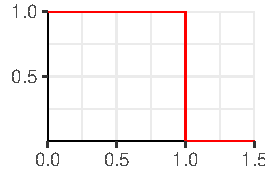
\includegraphics[scale=.66]{./img_ventanas/ventana_bartlett.pdf}
%\\
%\rowcolor{gris}
%Fejer &
%$\displaystyle 
%1-\abso{u}
%$
%& 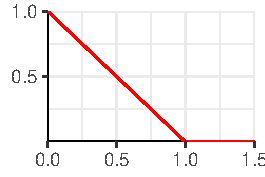
\includegraphics[scale=.66]{./img_ventanas/ventana_fejer.pdf}
%\\
%Daniell &
%$\displaystyle 
%\frac{\SEN{\pi u}}{\pi u}
%$
%& 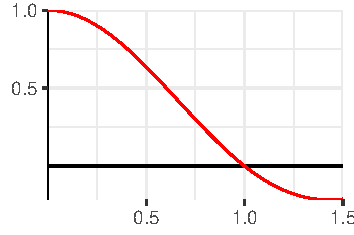
\includegraphics[scale=.66]{./img_ventanas/ventana_daniell.pdf}
%\\
%\rowcolor{gris}
%Parzen (1) &
%$\displaystyle 
%1-u^{2}
%$
%& 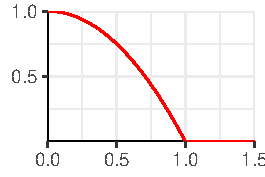
\includegraphics[scale=.66]{./img_ventanas/ventana_parzen1.pdf}
%\\
%Parzen (2) &
%$\displaystyle 
%\frac{1}{1+\abso{u}}
%$
%& 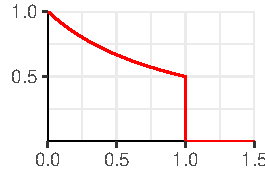
\includegraphics[scale=.66]{./img_ventanas/ventana_parzen2.pdf}
%\\
%\rowcolor{gris}
%Parzen (3) &
%$\displaystyle 
%\frac{1}{1+u^{2}}
%$
%& 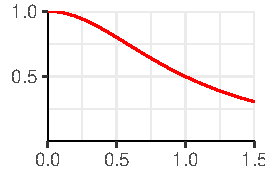
\includegraphics[scale=.66]{./img_ventanas/ventana_parzen3.pdf}
%\\
%Parzen (4) &
%$\displaystyle 
%\begin{cases}
%1-6 u^{2} + 6 \abso{u}^{3} &, \text{ si} \abso{u}\leq \nicefrac{1}{2}\\
%2\left( 1-\abso{u} \right)^{3} &, \text{ otro caso}
%\end{cases}
%$
%& 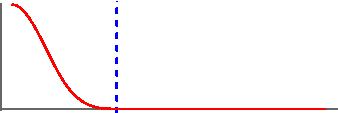
\includegraphics[scale=.66]{./img_ventanas/ventana_parzen4.pdf}
%\\
%\rowcolor{gris}
%Tukey &
%$\displaystyle 
%1 -2a +2a \COS{\pi u}
%$
%& 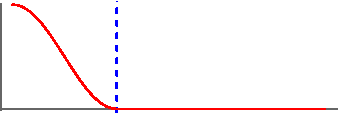
\includegraphics[scale=.66]{./img_ventanas/ventana_tukey.pdf}
%\\
%\bottomrulec
%\end{tabular}
%}
%\caption{Ejemplos de algunas ventanas que suavizan el periodograma}
%\label{ventanas}
%\end{SidewaysTable}

%%%%%%%%%%%%%%%%%%%%%%%%%%%%%%%%%%%%%%%%%%%%%%%%%%%%%%%%%%%%%%%%%%%%%%%%%%%%%%%%%%%%%%%%%%%%%%%%%%%

%\begin{SidewaysTable}
%\centering
%\bordes{1.5}
%\begin{tabular}{c}
%\textbf{Ventanas de retraso tipo escalamiento (2)}
%\vspace{1em}
%\end{tabular}
%
%{
%\begin{tabular}{lll}
%\toprule
%& $k(u)$ para $\abso{u} \leq 1$  & \\
%\midrule
%Neave &
%$\displaystyle 
%\begin{cases}
%1 &, \abso{u}\leq a \\
%\frac{1}{1-a}\left[ 1-u +\frac{b-a}{\pi}\SEN{\frac{b-u}{b-a}\pi} \right] &, a \leq \abso{u}\leq a \\
%\frac{1}{1-a}\left[ 1-u -\frac{1-b}{\pi}\SEN{\frac{u-b}{1-b}\pi} \right] &, b \leq \abso{u} \\
%\end{cases}
%$
%& 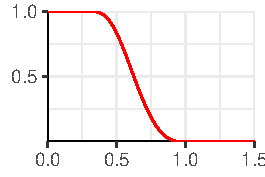
\includegraphics[scale=.66]{./img_ventanas/ventana_neave.pdf}
%\\
%\rowcolor{gris}
%Cuadrática &
%$\displaystyle 
%\frac{25}{12(\pi u)^{2}} 
%\left[ \frac{\SEN{\nicefrac{6 \pi u}{5}}}{\nicefrac{6\pi u}{5}} - \COS{\nicefrac{6 \pi u}{5}} \right]
%$
%& 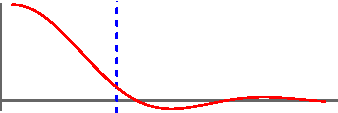
\includegraphics[scale=.66]{./img_ventanas/ventana_cuadratica.pdf}
%\\
%Bartlett-Priestley &
%$\displaystyle 
%\frac{3}{(\pi u)^{2}} \left[ \frac{\SEN{\pi u}}{\pi u} - \COS{\pi u} \right]
%$
%& 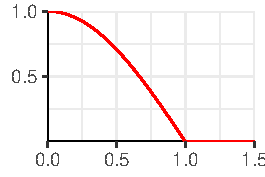
\includegraphics[scale=.66]{./img_ventanas/ventana_cosenoidal.pdf}
%\\
%\rowcolor{gris}
%Papoulis &
%$\displaystyle 
%(1-u)\COS{\pi u} + \frac{\SEN{\pi u }}{\pi u }
%$
%& 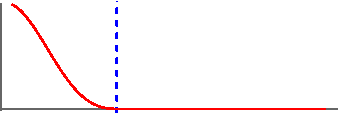
\includegraphics[scale=.66]{./img_ventanas/ventana_papoulis.pdf}
%\\
%Cosenoidal &
%$\displaystyle 
%\COS{\pi u}
%$
%\\
%\rowcolor{gris}
%Trapezoidal &
%$\displaystyle 
%\begin{cases}
%1 &, \abso{u}\leq a \\
%\frac{u-1}{a-1} &, a \leq \abso{u}\leq a 
%\end{cases}
%$
%& 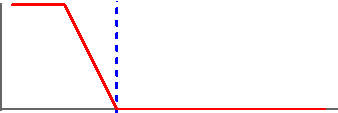
\includegraphics[scale=.66]{./img_ventanas/ventana_trapezoidal.pdf}
%\\
%Normal &
%$\displaystyle 
%\exp \left( - \nicefrac{u^{2}}{2 \sigma^{2}}  \right)
%$
%%& 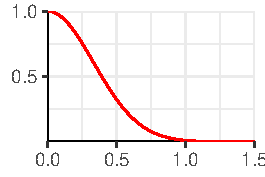
\includegraphics[scale=.66]{./img_ventanas/ventana_normal.pdf}
%& 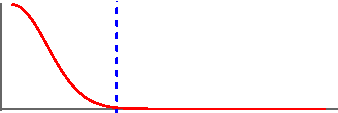
\includegraphics[scale=.66]{./img_ventanas/ventana_.pdf}
%\\
%\bottomrule
%\end{tabular}
%}
%\caption{Ejemplos de algunas ventanas que suavizan el periodograma}
%\end{SidewaysTable}

%%%%%%%%%%%%%%%%%%%%%%%%%%%%%%%%%%%%%%%%%%%%%%%%%%%%%%%%%%%%%%%%%%%%%%%%%%%%%%%%%%%%%%%%%%%%%%%%%%%
%%%%%%%%%%%%%%%%%%%%%%%%%%%%%%%%%%%%%%%%%%%%%%%%%%%%%%%%%%%%%%%%%%%%%%%%%%%%%%%%%%%%%%%%%%%%%%%%%%%
%%%%%%%%%%%%%%%%%%%%%%%%%%%%%%%%%%%%%%%%%%%%%%%%%%%%%%%%%%%%%%%%%%%%%%%%%%%%%%%%%%%%%%%%%%%%%%%%%%%

%\begin{SidewaysTable}
%\centering
%\bordes{1.5}
%\begin{tabular}{c}
%\textbf{Ventanas espectrales tipo escalamiento (1)}
%\vspace{1em}
%\end{tabular}
%
%{
%\begin{tabular}{ll}
%\toprule
%& $K(\theta)$ para $\abso{\theta} \leq 1$ \\
%\midrule
%Bartlett &
%$\displaystyle 
%\frac{1}{\pi} \frac{\SEN{\theta}}{\theta}
%$
%\\
%\rowcolor{gris}
%Fejer &
%$\displaystyle 
%\frac{1}{2\pi} \left[ \frac{\SEN{\nicefrac{\theta}{2}}}{\nicefrac{\theta}{2}} \right]^{2}
%$
%\\
%Daniell &
%$
%\displaystyle 
%\nicefrac{1}{2\pi} \text{, si } \abso{\theta}\leq \pi
%$
%\\
%\rowcolor{gris}
%Parzen (1) &
%$\displaystyle 
%d
%$
%\\
%Parzen (2) &
%$\displaystyle 
%d
%$
%\\
%\rowcolor{gris}
%Parzen (3) &
%$\displaystyle 
%d
%$
%\\
%Parzen (4) &
%$\displaystyle 
%\frac{3}{8 \pi} \left[ \frac{\SEN{\nicefrac{\theta}{4}}}{\nicefrac{\theta}{4}} \right]
%$
%\\
%\rowcolor{gris}
%Tukey &
%$\displaystyle 
%d
%$
%\\
%\bottomrulec
%\end{tabular}
%}
%\caption{Ejemplos de algunas ventanas que suavizan el periodograma}
%\end{SidewaysTable}

%%%%%%%%%%%%%%%%%%%%%%%%%%%%%%%%%%%%%%%%%%%%%%%%%%%%%%%%%%%%%%%%%%%%%%%%%%%%%%%%%%%%%%%%%%%%%%%%%%%

%\begin{SidewaysTable}
%\centering
%\bordes{1.5}
%\begin{tabular}{c}
%\textbf{Ventanas de retraso tipo escalamiento (2)}
%\vspace{1em}
%\end{tabular}
%
%{
%\begin{tabular}{ll}
%\toprule
%& $K(\theta)$ para $\abso{\theta} \leq 1$ \\
%\midrule
%Neave &
%$
%d
%$
%\\
%\rowcolor{gris}
%Cuadrática &
%$\displaystyle 
%d
%$
%\\
%Bartlett-Priestley &
%$\displaystyle 
%\frac{3}{4 \pi} \left[ 1 - \left( \nicefrac{\theta}{\pi} \right) \right]
%\text{, si } \abso{\theta}\leq \pi
%$
%\\
%\rowcolor{gris}
%Papoulis &
%$\displaystyle 
%d
%$
%\\
%Coseno &
%$\displaystyle 
%d
%$
%\\
%\rowcolor{gris}
%Trapezoidal &
%$\displaystyle 
%d
%$
%\\
%Normal &
%$\displaystyle 
%d
%$
%\\
%\bottomrule
%\end{tabular}
%}
%\caption{Ejemplos de algunas ventanas que suavizan el periodograma}
%%\label{ventanas}
%\end{SidewaysTable}

%%%%%%%%%%%%%%%%%%%%%%%%%%%%%%%%%%%%%%%%%%%%%%%%%%%%%%%%%%%%%%%%%%%%%%%%%%%%%%%%%%%%%%%%%%%%%%%%%%%
%%%%%%%%%%%%%%%%%%%%%%%%%%%%%%%%%%%%%%%%%%%%%%%%%%%%%%%%%%%%%%%%%%%%%%%%%%%%%%%%%%%%%%%%%%%%%%%%%%%
%%%%%%%%%%%%%%%%%%%%%%%%%%%%%%%%%%%%%%%%%%%%%%%%%%%%%%%%%%%%%%%%%%%%%%%%%%%%%%%%%%%%%%%%%%%%%%%%%%%
%%%%%%%%%%%%%%%%%%%%%%%%%%%%%%%%%%%%%%%%%%%%%%%%%%%%%%%%%%%%%%%%%%%%%%%%%%%%%%%%%%%%%%%%%%%%%%%%%%%

%%%%%%%%%%%%%%%%%%%%%%%%%%%%%%%%%%%%%%%%%%%%%%%%%%%%%%%%%%%%%%%%%%%%%%%%%%%%%%%%%%%%%%%%%%%%%%%%%%%
%%%%%%%%%%%%%%%%%%%%%%%%%%%%%%%%%%%%%%%%%%%%%%%%%%%%%%%%%%%%%%%%%%%%%%%%%%%%%%%%%%%%%%%%%%%%%%%%%%%
%%%%%%%%%%%%%%%%%%%%%%%%%%%%%%%%%%%%%%%%%%%%%%%%%%%%%%%%%%%%%%%%%%%%%%%%%%%%%%%%%%%%%%%%%%%%%%%%%%%
%%%%%%%%%%%%%%%%%%%%%%%%%%%%%%%%%%%%%%%%%%%%%%%%%%%%%%%%%%%%%%%%%%%%%%%%%%%%%%%%%%%%%%%%%%%%%%%%%%%

\chapter{Espectro evolutivo}

%%%%%%%%%%%%%%%%%%%%%%%%%%%%%%%%%%%%%%%%%%%%%%%%%%%%%%%%%%%%%%%%%%%%%%%%%%%%%%%%%%%%%%%%%%%%%%%%%%%

\section{Espectro evolutivo}

\begin{proposicion}
Sean $u$ y $v$ dos funciones tipo \textit{pseudo $\delta$ de Dirac}, es decir, unimodales con un
máximo  y (...). Si $u$ tiene una concentración muy alta, con relación a $v$, entonces
\begin{equation*}
\intR u(x) v(x+k) dx \approx v(k) \intR u(x) dx
\end{equation*}
\label{pseudo_d}
\end{proposicion}

%%%%%%%%%%%%%%%%%%%%%%%%%%%%%%%%%%%%%%%%%%%%%%%%%%%%%%%%%%%%%%%%%%%%%%%%%%%%%%%%%%%%%%%%%%%%%%%%%%%
%%%%%%%%%%%%%%%%%%%%%%%%%%%%%%%%%%%%%%%%%%%%%%%%%%%%%%%%%%%%%%%%%%%%%%%%%%%%%%%%%%%%%%%%%%%%%%%%%%%
%%%%%%%%%%%%%%%%%%%%%%%%%%%%%%%%%%%%%%%%%%%%%%%%%%%%%%%%%%%%%%%%%%%%%%%%%%%%%%%%%%%%%%%%%%%%%%%%%%%

%\begin{SidewaysTable}
%\centering
%\bordes{1.5}
%\begin{tabular}{c}
%\textbf{Ventanas de retrasos tipo escalamiento (1)}
%\vspace{1em}
%\end{tabular}
%
%{
%\begin{tabular}{lll}
%\toprule
%& $k(u)$ para $\abso{u} \leq 1$ & \\
%\midrule
%Bartlett &
%$\displaystyle 
%1 
%$
%& \includegraphics[scale=.66]{./img_ventanas/ventana_bartlett.pdf}
%\\
%\rowcolor{gris}
%Fejer &
%$\displaystyle 
%1-\abso{u}
%$
%& \includegraphics[scale=.66]{./img_ventanas/ventana_fejer.pdf}
%\\
%Daniell &
%$\displaystyle 
%\frac{\SEN{\pi u}}{\pi u}
%$
%& \includegraphics[scale=.66]{./img_ventanas/ventana_daniell.pdf}
%\\
%\rowcolor{gris}
%Parzen (1) &
%$\displaystyle 
%1-u^{2}
%$
%& \includegraphics[scale=.66]{./img_ventanas/ventana_parzen1.pdf}
%\\
%Parzen (2) &
%$\displaystyle 
%\frac{1}{1+\abso{u}}
%$
%& \includegraphics[scale=.66]{./img_ventanas/ventana_parzen2.pdf}
%\\
%\rowcolor{gris}
%Parzen (3) &
%$\displaystyle 
%\frac{1}{1+u^{2}}
%$
%& \includegraphics[scale=.66]{./img_ventanas/ventana_parzen3.pdf}
%\\
%Parzen (4) &
%$\displaystyle 
%\begin{cases}
%1-6 u^{2} + 6 \abso{u}^{3} &, \text{ si} \abso{u}\leq \nicefrac{1}{2}\\
%2\left( 1-\abso{u} \right)^{3} &, \text{ otro caso}
%\end{cases}
%$
%& \includegraphics[scale=.66]{./img_ventanas/ventana_parzen4.pdf}
%\\
%\rowcolor{gris}
%Tukey &
%$\displaystyle 
%1 -2a +2a \COS{\pi u}
%$
%& \includegraphics[scale=.66]{./img_ventanas/ventana_tukey.pdf}
%\\
%\bottomrulec
%\end{tabular}
%}
%\caption{Ejemplos de algunas ventanas que suavizan el periodograma}
%\label{ventanas}
%\end{SidewaysTable}

%%%%%%%%%%%%%%%%%%%%%%%%%%%%%%%%%%%%%%%%%%%%%%%%%%%%%%%%%%%%%%%%%%%%%%%%%%%%%%%%%%%%%%%%%%%%%%%%%%%

%\begin{SidewaysTable}
%\centering
%\bordes{1.5}
%\begin{tabular}{c}
%\textbf{Ventanas de retraso tipo escalamiento (2)}
%\vspace{1em}
%\end{tabular}
%
%{
%\begin{tabular}{lll}
%\toprule
%& $k(u)$ para $\abso{u} \leq 1$  & \\
%\midrule
%Neave &
%$\displaystyle 
%\begin{cases}
%1 &, \abso{u}\leq a \\
%\frac{1}{1-a}\left[ 1-u +\frac{b-a}{\pi}\SEN{\frac{b-u}{b-a}\pi} \right] &, a \leq \abso{u}\leq a \\
%\frac{1}{1-a}\left[ 1-u -\frac{1-b}{\pi}\SEN{\frac{u-b}{1-b}\pi} \right] &, b \leq \abso{u} \\
%\end{cases}
%$
%& \includegraphics[scale=.66]{./img_ventanas/ventana_neave.pdf}
%\\
%\rowcolor{gris}
%Cuadrática &
%$\displaystyle 
%\frac{25}{12(\pi u)^{2}} 
%\left[ \frac{\SEN{\nicefrac{6 \pi u}{5}}}{\nicefrac{6\pi u}{5}} - \COS{\nicefrac{6 \pi u}{5}} \right]
%$
%& \includegraphics[scale=.66]{./img_ventanas/ventana_cuadratica.pdf}
%\\
%Bartlett-Priestley &
%$\displaystyle 
%\frac{3}{(\pi u)^{2}} \left[ \frac{\SEN{\pi u}}{\pi u} - \COS{\pi u} \right]
%$
%& \includegraphics[scale=.66]{./img_ventanas/ventana_cosenoidal.pdf}
%\\
%\rowcolor{gris}
%Papoulis &
%$\displaystyle 
%(1-u)\COS{\pi u} + \frac{\SEN{\pi u }}{\pi u }
%$
%& \includegraphics[scale=.66]{./img_ventanas/ventana_papoulis.pdf}
%\\
%Cosenoidal &
%$\displaystyle 
%\COS{\pi u}
%$
%\\
%\rowcolor{gris}
%Trapezoidal &
%$\displaystyle 
%\begin{cases}
%1 &, \abso{u}\leq a \\
%\frac{u-1}{a-1} &, a \leq \abso{u}\leq a 
%\end{cases}
%$
%& \includegraphics[scale=.66]{./img_ventanas/ventana_trapezoidal.pdf}
%\\
%Normal &
%$\displaystyle 
%\exp \left( - \nicefrac{u^{2}}{2 \sigma^{2}}  \right)
%$
%%& \includegraphics[scale=.66]{./img_ventanas/ventana_normal.pdf}
%& \includegraphics[scale=.66]{./img_ventanas/ventana_.pdf}
%\\
%\bottomrule
%\end{tabular}
%}
%\caption{Ejemplos de algunas ventanas que suavizan el periodograma}
%\end{SidewaysTable}

%%%%%%%%%%%%%%%%%%%%%%%%%%%%%%%%%%%%%%%%%%%%%%%%%%%%%%%%%%%%%%%%%%%%%%%%%%%%%%%%%%%%%%%%%%%%%%%%%%%
%%%%%%%%%%%%%%%%%%%%%%%%%%%%%%%%%%%%%%%%%%%%%%%%%%%%%%%%%%%%%%%%%%%%%%%%%%%%%%%%%%%%%%%%%%%%%%%%%%%
%%%%%%%%%%%%%%%%%%%%%%%%%%%%%%%%%%%%%%%%%%%%%%%%%%%%%%%%%%%%%%%%%%%%%%%%%%%%%%%%%%%%%%%%%%%%%%%%%%%

%\begin{SidewaysTable}
%\centering
%\bordes{1.5}
%\begin{tabular}{c}
%\textbf{Ventanas espectrales tipo escalamiento (1)}
%\vspace{1em}
%\end{tabular}
%
%{
%\begin{tabular}{ll}
%\toprule
%& $K(\theta)$ para $\abso{\theta} \leq 1$ \\
%\midrule
%Bartlett &
%$\displaystyle 
%\frac{1}{\pi} \frac{\SEN{\theta}}{\theta}
%$
%\\
%\rowcolor{gris}
%Fejer &
%$\displaystyle 
%\frac{1}{2\pi} \left[ \frac{\SEN{\nicefrac{\theta}{2}}}{\nicefrac{\theta}{2}} \right]^{2}
%$
%\\
%Daniell &
%$
%\displaystyle 
%\nicefrac{1}{2\pi} \text{, si } \abso{\theta}\leq \pi
%$
%\\
%\rowcolor{gris}
%Parzen (1) &
%$\displaystyle 
%d
%$
%\\
%Parzen (2) &
%$\displaystyle 
%d
%$
%\\
%\rowcolor{gris}
%Parzen (3) &
%$\displaystyle 
%d
%$
%\\
%Parzen (4) &
%$\displaystyle 
%\frac{3}{8 \pi} \left[ \frac{\SEN{\nicefrac{\theta}{4}}}{\nicefrac{\theta}{4}} \right]
%$
%\\
%\rowcolor{gris}
%Tukey &
%$\displaystyle 
%d
%$
%\\
%\bottomrulec
%\end{tabular}
%}
%\caption{Ejemplos de algunas ventanas que suavizan el periodograma}
%\end{SidewaysTable}

%%%%%%%%%%%%%%%%%%%%%%%%%%%%%%%%%%%%%%%%%%%%%%%%%%%%%%%%%%%%%%%%%%%%%%%%%%%%%%%%%%%%%%%%%%%%%%%%%%%

%\begin{SidewaysTable}
%\centering
%\bordes{1.5}
%\begin{tabular}{c}
%\textbf{Ventanas de retraso tipo escalamiento (2)}
%\vspace{1em}
%\end{tabular}
%
%{
%\begin{tabular}{ll}
%\toprule
%& $K(\theta)$ para $\abso{\theta} \leq 1$ \\
%\midrule
%Neave &
%$
%d
%$
%\\
%\rowcolor{gris}
%Cuadrática &
%$\displaystyle 
%d
%$
%\\
%Bartlett-Priestley &
%$\displaystyle 
%\frac{3}{4 \pi} \left[ 1 - \left( \nicefrac{\theta}{\pi} \right) \right]
%\text{, si } \abso{\theta}\leq \pi
%$
%\\
%\rowcolor{gris}
%Papoulis &
%$\displaystyle 
%d
%$
%\\
%Coseno &
%$\displaystyle 
%d
%$
%\\
%\rowcolor{gris}
%Trapezoidal &
%$\displaystyle 
%d
%$
%\\
%Normal &
%$\displaystyle 
%d
%$
%\\
%\bottomrule
%\end{tabular}
%}
%\caption{Ejemplos de algunas ventanas que suavizan el periodograma}
%%\label{ventanas}
%\end{SidewaysTable}

%%%%%%%%%%%%%%%%%%%%%%%%%%%%%%%%%%%%%%%%%%%%%%%%%%%%%%%%%%%%%%%%%%%%%%%%%%%%%%%%%%%%%%%%%%%%%%%%%%%

\section{Estimación del espectro evolutivo}

Una vez definido el espectro evolutivo para procesos no-estacionarios con varianza finita, cabe 
preguntarse sobre le estimación de esta cantidad a partir de una realización del proceso usando, 
por ejemplo, periodogramas modificados; tal pregunta no tiene, en general, una respuesta 
satisfactoria.
Es por ello que se define una colección, más restringida, de procesos no-estacionarios cuyo 
espectro evolutivo pueda ser estimado efectivamente usando la técnica de ventanas.

Considerando un proceso no-estacionario \xt que admite una representación de la forma 
$X(t) = \intR A(t,\omega) e^{i \omega t} dZ(\omega)$, entonces el espectro evolutivo queda definido 
como
\begin{equation}
dF_t(\omega) = \abso{A(t,\omega)}^{2} d\mu(\omega)
\label{esp_evolutivo}
\end{equation}

Antes de poder usar la proposición \ref{pseudo_d} para estimar $F_t$ (con respecto a $t$) usando 
una ventana espectral, hay que medir la dispersión de $F_t$ en el tiempo; más aún, hay que pedir 
que esa dispersión sea finita.
Con vista a la ecuación \ref{esp_evolutivo}, se puede usar la conexión entre $F$ y $A$ para 
establecer condiciones respecto a la segunda; se define entonces a $H_\omega$, la transformada de
Fourier de $A$ en el tiempo
\begin{equation}
A(t,\omega) = \intR e^{i t \theta} dH_\omega(\theta)
\end{equation}

Un motivo muy fuerte para definir un objeto tan rebuscado es que (...)

Posteriormente se define a $B_{\mathbf{F}}$, el ancho de banda para $H_\omega$ con respecto a la 
familia de funciones $\mathbf{F}$, como
%
\begin{equation}
B_{\mathbf{F}}(\omega) = \intR \abso{\theta} \abso{dH_\omega(\theta)}
\end{equation}

Se dice que el proceso es semi-estacionario con respecto a $\mathbf{F}$ si 
$\sup_\omega B_{\mathbf{F}} < \infty$. El proceso se dice simplemente \textbf{semi-estacionario} 
si esta cantidad es acotada para cualquier familia de funciones admisibles 
$\mathbf{F} \in \mathbf{C}$; entonces se puede definir la constante $B_X$, el \textit{ancho de 
banda característico de} \xt, como

\begin{equation}
B_X = \sup_{\mathbf{F}\in \mathbf{C}} \left[ \sup_\omega B_{\mathbf{F}}(\omega) \right]^{-1}
\end{equation}

Muy vagamente, $B_X$ indica el tiempo máximo en el cual el proceso, representado en la forma
\ref{esp_evolutivo}, (...)

Una vez definida la cantidad $B_X$, y habiendo supuesto que no es 0, es demostrado en 
\cite{Priestley65} que el estimador $U$ definido como en ... satisface que
%
\begin{equation}
\E{\abso{U(t,\omega)}^{2}} = \intR \abso{\Gamma(\omega)}^{2} f(t,\omega+\omega_0) d\omega
+ \orden\left( \nicefrac{B_g}{B_X} \right)
\end{equation}

De esta última expresión es evidente que el estimador es mejor conforme 
\begin{itemize}
\item  $B_X$, el tiempo máximo para el cual el proceso es \textit{básicamente estacionario}, es 
mayor
\item $B_g$, la dispersión en el tiempo para la ventana $g$, es menor
\end{itemize}

---

Entonces se ha probado en \cite{Priestley66,Priestley69} que bajo ciertas
condiciones p

\section{Estimador de doble ventana}

Respecto a la estimación del espectro local se usa el \textbf{estimador de doble ventana}, 
técnica introducida por Priestley \cite{Priestley69} y que requiere dos funciones, $w_\tau$ y 
$g$, que funcionan como ventana de retrasos y como filtro lineal, respectivamente.
%
En cuando a $g$, se define a $\Gamma(u) = \intR g(u) e^{i u \omega} du$ y se les pide que
\begin{equation*}
2\pi \int_{-\infty}^{\infty} \lvert g(u) \lvert^{2} du 
= 
\int_{-\infty}^{\infty} \lvert \Gamma(\omega) \lvert^{2} d\omega
= 1
\end{equation*}

Cabe mencionar que las ventanas espectrales mostradas en la tabla \ref{ventanas} bien 
pueden cumplir las propiedades requeridas para ser filtros.
Posteriormente se define el estimador $U$ con el objetivo de asignar pesos en el tiempo para estimar
a la FDE
% en el tiempo dado; más aún, $U$ sirve 
%como una aproximación de la representación de Wold-Cramér para 
%el proceso.
\begin{equation*}
U(t,\omega) = \int_{t-T}^{t} g(u) X({t-u}) e^{i \omega (t-u)} du
\end{equation*}

Bajo el entendido que la función $\Gamma$ converge a una función tipo \dirac, puede 
considerarse que 
$\E{\abso{U(t,\omega)}^{2}} \approx f_t(\omega)$; sin embargo, se demuestra en \cite{Priestley66} 
que $\Var{\abso{U(t,\omega)}^{2}} \nrightarrow 0$.
%
Debido a ello se usa una segunda función tipo ventana,
%, para 'suavizar' el estimador y hacerlo consistente (
de forma similar al periodograma.
Se considera la función $W_\tau$, ventana de retrasos, y su respectiva ventana espectral 
$w_\tau$; deben satisfacer las siguientes propiedades:
\begin{itemize}
\item $w_{\tau}(t) \geq 0$ para cualesquiera $t$, $\tau$
\item $w_{\tau}(t) \rightarrow 0$ cuando $\lvert t \lvert \rightarrow \infty$, para todo $\tau$
\item $\displaystyle \int_{-\infty}^{\infty} w_{\tau}(t) dt = 1$ para todo $\tau$
\item $\displaystyle \int_{-\infty}^{\infty} \left( w_{\tau}(t) \right)^{2} dt < \infty$ para todo $\tau$
\item $\exists C$ tal que  
$\displaystyle \lim_{\tau\rightarrow\infty} \tau \int_{-\infty}^{t} \abso{ W_{\tau}(\lambda) }^{2} d\lambda = C$
\end{itemize}

%Por ejemplo, la ventana de Daniell satisface estas propiedades; para ello, conviene calcular que
%$\lim_{\tau\rightarrow\infty} \tau \int_{t-T}^{t} \lvert W_{\tau}(\lambda) \lvert^{2} d\lambda = 2\pi$;
%más aún, 
Cabe mencionar que todas las ventanas mostradas en \ref{ventanas} satisfacen las propiedades 
anteriores.
Finalmente, se define el estimador $\est{f}$ para las FDE normalizada, $f_t$, como
\begin{equation*}
\widehat{f}(t,\omega) = \int_{t-T}^{t} w_{T'}(u) \lvert U(t-u,\omega) \lvert^{2} du
\label{estimador_doble_ventana}
\end{equation*}

Fue demostrado por Priestley \cite{Priestley65} que los estimadores de doble ventana son 
asintóticamente insesgados y consistentes, y propone las siguientes aproximaciones:
%conviene exhibir las siguientes expresiones aproximadas propuestas en aquél trabajo
\begin{itemize}
\item $\displaystyle
\E{\est{f}(t,\omega)} \approx 
\intR \widetilde{f}(t,\omega+\theta) \abso{\Gamma(\theta)}^{2} d\theta$
\item $\displaystyle
\Var{\est{f}(t,\omega)} \approx \frac{C}{\tau} \left( \overline{f}^{2}(\omega) \right)
\intR \abso{\Gamma(\theta)}^{4} d\theta $
\end{itemize}

donde las funciones $\widetilde{f}$ y $\overline{f}$ son versiones 'suavizadas' de la FDE 
normalizada, $f$, y están definidas de la siguiente manera
\begin{equation*}
\widetilde{f}(t,\omega+\theta) = 
\intR W_{\tau}(u) f(t-u,\omega+\theta) du
\end{equation*}
\begin{equation*}
\overline{f}^{2} (t,\omega) =
\frac{\intR f^{2}\left(t-u,W_{\tau}^{2}(u)\right) du}
{\intR \left( W_{\tau}(u) \right)^{2} du}
\end{equation*}

Como $W_{\tau}$ funciona como ventana espectral, converge a una 
función tipo \dirac; luego $\widetilde{f}$ es aproximadamente la convolución 
$\widetilde{f}(t,\omega+\theta) \approx \delta_t \ast f(\bullet,\omega+\theta)$. 
Una aproximación muy similar 
puede hacerse respecto al segundo término, de modo que $\widetilde{f}\approx f$ y 
$\overline{f}^{2}\approx f^{2}$.
Tales aproximaciones serán mejores en tanto las ventanas $w_{\tau}$ y $W_{\tau}$ sean más 
cercanas a funciones tipo \dirac.
%; más aún, una condición adecuada es que estas funciones 
%tengan una forma 'más delgada' que el espacio entre los tiempos y frecuencias donde se estimará 
%$f$.
Dicho esto, se pueden hacer las siguientes aproximaciones, un poco más arriesgadas:
\begin{itemize}
\item $\displaystyle \E{\est{f}(t,\omega)} \approx f(t,\omega)$
\item $\displaystyle \Var{\est{f}(t,\omega)} \approx 
\frac{C}{\tau} f^{2}(t,\omega) \intR \abso{\Gamma (\theta)}^{4} d\theta$
\end{itemize}

%%%%%%%%%%%%%%%%%%%%%%%%%%%%%%%%%%%%%%%%%%%%%%%%%%%%%%%%%%%%%%%%%%%%%%%%%%%%%%%%%%%%%%%%%%%%%%%%%%%
%%%%%%%%%%%%%%%%%%%%%%%%%%%%%%%%%%%%%%%%%%%%%%%%%%%%%%%%%%%%%%%%%%%%%%%%%%%%%%%%%%%%%%%%%%%%%%%%%%%

%\section{Efecto del filtro STL}

%%%%%%%%%%%%%%%%%%%%%%%%%%%%%%%%%%%%%%%%%%%%%%%%%%%%%%%%%%%%%%%%%%%%%%%%%%%%%%%%%%%%%%%%%%%%%%%%%%%
%%%%%%%%%%%%%%%%%%%%%%%%%%%%%%%%%%%%%%%%%%%%%%%%%%%%%%%%%%%%%%%%%%%%%%%%%%%%%%%%%%%%%%%%%%%%%%%%%%%
%%%%%%%%%%%%%%%%%%%%%%%%%%%%%%%%%%%%%%%%%%%%%%%%%%%%%%%%%%%%%%%%%%%%%%%%%%%%%%%%%%%%%%%%%%%%%%%%%%%
%%%%%%%%%%%%%%%%%%%%%%%%%%%%%%%%%%%%%%%%%%%%%%%%%%%%%%%%%%%%%%%%%%%%%%%%%%%%%%%%%%%%%%%%%%%%%%%%%%%

%%%%%%%%%%%%%%%%%%%%%%%%%%%%%%%%%%%%%%%%%%%%%%%%%%%%%%%%%%%%%%%%%%%%%%%%%%%%%%%%%%%%%%%%%%%%%%%%%%%%
%%%%%%%%%%%%%%%%%%%%%%%%%%%%%%%%%%%%%%%%%%%%%%%%%%%%%%%%%%%%%%%%%%%%%%%%%%%%%%%%%%%%%%%%%%%%%%%%%%%
%%%%%%%%%%%%%%%%%%%%%%%%%%%%%%%%%%%%%%%%%%%%%%%%%%%%%%%%%%%%%%%%%%%%%%%%%%%%%%%%%%%%%%%%%%%%%%%%%%%
%%%%%%%%%%%%%%%%%%%%%%%%%%%%%%%%%%%%%%%%%%%%%%%%%%%%%%%%%%%%%%%%%%%%%%%%%%%%%%%%%%%%%%%%%%%%%%%%%%%

\chapter{Electrofisiología del polisomnograma}



%%%%%%%%%%%%%%%%%%%%%%%%%%%%%%%%%%%%%%%%%%%%%%%%%%%%%%%%%%%%%%%%%%%%%%%%%%%%%%%%%%%%%%%%%%%%%%%%%%%
%%%%%%%%%%%%%%%%%%%%%%%%%%%%%%%%%%%%%%%%%%%%%%%%%%%%%%%%%%%%%%%%%%%%%%%%%%%%%%%%%%%%%%%%%%%%%%%%%%%
%%%%%%%%%%%%%%%%%%%%%%%%%%%%%%%%%%%%%%%%%%%%%%%%%%%%%%%%%%%%%%%%%%%%%%%%%%%%%%%%%%%%%%%%%%%%%%%%%%%
%%%%%%%%%%%%%%%%%%%%%%%%%%%%%%%%%%%%%%%%%%%%%%%%%%%%%%%%%%%%%%%%%%%%%%%%%%%%%%%%%%%%%%%%%%%%%%%%%%%

%\input{./texto/eeg.tex}

%%%%%%%%%%%%%%%%%%%%%%%%%%%%%%%%%%%%%%%%%%%%%%%%%%%%%%%%%%%%%%%%%%%%%%%%%%%%%%%%%%%%%%%%%%%%%%%%%%%
%%%%%%%%%%%%%%%%%%%%%%%%%%%%%%%%%%%%%%%%%%%%%%%%%%%%%%%%%%%%%%%%%%%%%%%%%%%%%%%%%%%%%%%%%%%%%%%%%%%
%%%%%%%%%%%%%%%%%%%%%%%%%%%%%%%%%%%%%%%%%%%%%%%%%%%%%%%%%%%%%%%%%%%%%%%%%%%%%%%%%%%%%%%%%%%%%%%%%%%
%%%%%%%%%%%%%%%%%%%%%%%%%%%%%%%%%%%%%%%%%%%%%%%%%%%%%%%%%%%%%%%%%%%%%%%%%%%%%%%%%%%%%%%%%%%%%%%%%%%

\chapter{Tablas}

En este ap\'endice se incluyen las gr\'aficas y tablas obtenidas durante el trabajo; todos ellos 
son referidos en la secci\'on de Resultados, pero son presentados como ap\'endice a fin de resaltar 
en el texto las conclusiones obtenidas.

En las primeras tres tablas (\ref{total_gpos_mor}, \ref{total_gpos_nmor}, \ref{total_gpos_total}) 
se muestra el n\'umero total de \'epocas clasificadas como PE para cada sujeto y cada canal para 
las diferentes etapas de sue\~no. En las siguientes tablas (\ref{gpos_mor}, \ref{gpos_nmor}, 
\ref{gpos_total}) se exhibe la misma informaci\'on pero como proporciones, a modo de 
normalizaci\'on entre los diferentes sujetos. Se muestran promedios y desviaciones est\'andar por 
cada grupo.

Posteriormente, en la tabla \ref{comparacion_mor_vs_total} se muestran los resultados de comparar 
la proporci\'on de \'epocas PE durante MOR y NMOR; este an\'alisis se hizo individualmente por cada
sujeto usando la prueba $\chi^{2}$ para proporciones.

%%%%%%%%%%%%%%%%%%%%%%%%%%%%%%%%%%%%%%%%%%%%%%%%%%%%%%%%%%%%%%%%%%%%%%%%%%%%%%%%%%%%%%%%%%%%%%%%%%%

\begin{SidewaysTable}
\centering
\begin{tabular}{c}
\textbf{\'epocas clasificadas como PE, sue\~no MOR}
\vspace{1em}
\end{tabular}
\begin{tabular}{lrrrrrcrrrrcrrr}
\toprule
& \multicolumn{5}{c}{\textbf{Gpo. Control}} && 
  \multicolumn{4}{c}{\textbf{Gpo. PDC}} && 
  \multicolumn{3}{c}{\textbf{Excluidos}}\\
\cmidrule{2-6} \cmidrule{8-11} \cmidrule{13-15}
& \textbf{VCR} & \textbf{MJH} & \textbf{JAE} & \textbf{GHA} & \textbf{MFGR} & \phantom{l}
& \textbf{CLO} & \textbf{RLO} & \textbf{RRU} & \textbf{JGZ} & \phantom{l}
& \textbf{FGH} & \textbf{MGG} & \textbf{EMT} \\
\midrule
\textbf{C3} &6 &18&10&1 &12&&6 &35&16&1 &&2 &28&22 \\
\textbf{C4} &7 &16&4 &2 &10&&4 &40&5 &0 &&1 &23&26 \\
\textbf{CZ} &2 &16&13&2 &8 &&5 &22&4 &1 &&1 &13&19 \\
\rowcolor{gris}
\textbf{F3} &5 &23&10&0 &3 &&7 &43&3 &3 &&6 &14&20 \\
\rowcolor{gris}
\textbf{F4} &11&23&5 &1 &1 &&6 &36&5 &0 &&0 &4 &24 \\
\rowcolor{gris}
\textbf{F7} &5 &15&2 &0 &4 &&1 &18&0 &0 &&0 &2 &24 \\
\rowcolor{gris}
\textbf{F8} &4 &11&6 &1 &3 &&4 &23&1 &0 &&0 &2 &20 \\
\textbf{FP1}&2 &7 &1 &0 &1 &&0 &0 &1 &0 &&22&0 &22 \\
\textbf{FP2}&1 &6 &3 &0 &2 &&1 &15&1 &0 &&0 &1 &18 \\
\textbf{FZ} &11&18&19&0 &6 &&7 &38&2 &2 &&0 &20&23 \\
\rowcolor{gris}
\textbf{O1} &10&20&5 &3 &23&&2 &25&9 &2 &&5 &18&19 \\
\rowcolor{gris}
\textbf{O2} &13&23&3 &3 &21&&3 &34&9 &1 &&1 &12&16 \\
\textbf{P3} &6 &17&2 &2 &26&&5 &33&8 &0 &&1 &24&17 \\
\textbf{P4} &4 &19&4 &5 &18&&4 &27&5 &1 &&4 &15&21 \\
\textbf{PZ} &4 &15&5 &3 &22&&4 &32&4 &0 &&1 &8 &20 \\
\rowcolor{gris}
\textbf{T3} &10&29&1 &8 &26&&10&34&4 &0 &&2 &29&31 \\
\rowcolor{gris}
\textbf{T4} &12&20&2 &3 &21&&3 &35&6 &1 &&0 &10&17 \\
\rowcolor{gris}
\textbf{T5} &10&26&0 &3 &27&&5 &34&5 &2 &&2 &31&19 \\
\rowcolor{gris}
\textbf{T6} &15&18&3 &15&20&&3 &24&4 &2 &&0 &9 &19 \\
\textbf{LOG}&6 &20&8 &0 &9 &&5 &11&2 &0 &&1 &8 &30 \\
\textbf{ROG}&6 &21&17&2 &11&&9 &7 &4 &1 &&0 &19&33 \\
\textbf{EMG}&14&11&0 &0 &17&&14&16&4 &0 &&0&3&7 \\
\rowcolor{gris2}
\textbf{Total}&73&127&171&55&95&&132&99&38&33&&22&166&47 \\
\bottomrule
\end{tabular}
\caption{Total de \'epocas clasificadas como PE en sue\~no MOR, desglosado por canal. En la 
\'ultima fila se reporta el total de \'epocas de sue\~no MOR.
}
\label{total_gpos_mor}
\end{SidewaysTable}

%%%%%%%%%%%%%%%%%%%%%%%%%%%%%%%%%%%%%%%%%%%%%%%%%%%%%%%%%%%%%%%%%%%%%%%%%%%%%%%%%%%%%%%%%%%%%%%%%%%

\begin{SidewaysTable}
\centering
\begin{tabular}{c}
\textbf{\'epocas clasificadas como PE, sue\~no NMOR}
\vspace{1em}
\end{tabular}
\begin{tabular}{lrrrrrcrrrrcrrr}
\toprule
& \multicolumn{5}{c}{\textbf{Gpo. Control}} && 
  \multicolumn{4}{c}{\textbf{Gpo. PDC}} && 
  \multicolumn{3}{c}{\textbf{Excluidos}}\\
\cmidrule{2-6} \cmidrule{8-11} \cmidrule{13-15}
& \textbf{VCR} & \textbf{MJH} & \textbf{JAE} & \textbf{GHA} & \textbf{MFGR} & \phantom{l}
& \textbf{CLO} & \textbf{RLO} & \textbf{RRU} & \textbf{JGZ} & \phantom{l}
& \textbf{FGH} & \textbf{MGG} & \textbf{EMT} \\
\midrule
\textbf{C3} &187&135&100&175&112&&55 &153&76 &56 &&16 &201&478 \\
\textbf{C4} &168&129&89 &156&87 &&36 &135&94 &47 &&7  &207&598 \\
\textbf{CZ} &167&131&88 &107&77 &&54 &145&69 &62 &&8  &180&518 \\
\rowcolor{gris}
\textbf{F3} &168&134&83 &150&73 &&57 &175&79 &68 &&107&143&331 \\
\rowcolor{gris}
\textbf{F4} &180&132&55 &146&24 &&41 &135&80 &49 &&0  &137&549 \\
\rowcolor{gris}
\textbf{F7} &158&137&77 &213&87 &&45 &112&68 &58 &&0  &152&262 \\
\rowcolor{gris}
\textbf{F8} &157&123&30 &168&36 &&41 &96 &86 &48 &&0  &128&574 \\
\textbf{FP1}&163&75 &23 &128&65 &&34 &0  &71 &44 &&381&169&518 \\
\textbf{FP2}&156&82 &44 &116&21 &&33 &99 &26 &44 &&0  &146&449 \\
\textbf{FZ} &170&134&78 &156&51 &&55 &163&91 &65 &&0  &177&533 \\
\rowcolor{gris}
\textbf{O1} &202&174&51 &295&175&&48 &150&92 &96 &&20 &140&675 \\
\rowcolor{gris}
\textbf{O2} &166&165&63 &247&173&&32 &136&70 &106&&22 &161&573 \\
\textbf{P3} &175&122&53 &288&132&&72 &147&108&95 &&29 &212&490 \\
\textbf{P4} &180&136&108&252&140&&56 &135&110&73 &&18 &206&495 \\
\textbf{PZ} &156&131&90 &216&112&&57 &167&112&59 &&15 &177&497 \\
\rowcolor{gris}
\textbf{T3} &181&140&52 &230&171&&81 &112&80 &102&&27 &115&603 \\
\rowcolor{gris}
\textbf{T4} &181&121&35 &182&128&&26 &110&112&87 &&10 &122&531 \\
\rowcolor{gris}
\textbf{T5} &218&146&16 &265&199&&78 &137&104&61 &&19 &208&621 \\
\rowcolor{gris}
\textbf{T6} &218&148&49 &194&181&&38 &118&98 &84 &&18 &209&558 \\
\textbf{LOG}&236&224&214&287&170&&144&185&128&225&&50 &437&820 \\
\textbf{ROG}&236&205&212&334&159&&126&179&110&225&&67 &455&873 \\
\textbf{EMG}&94 &62 &16 &1  &157&&20 &82 &110&10 &&1  &55 &266 \\
\rowcolor{gris2}
\textbf{Total}&788&905&736&1038&727&&812&747&376&1174&&383&864&1376 \\
\bottomrule
\end{tabular}
\caption{Total de \'epocas clasificadas como PE en sue\~no NMOR, desglosado por canal. 
En la \'ultima fila se reporta el total de \'epocas en sue\~no NMOR.
}
\label{total_gpos_nmor}
\end{SidewaysTable}

%%%%%%%%%%%%%%%%%%%%%%%%%%%%%%%%%%%%%%%%%%%%%%%%%%%%%%%%%%%%%%%%%%%%%%%%%%%%%%%%%%%%%%%%%%%%%%%%%%%

\begin{SidewaysTable}
\centering
\begin{tabular}{c}
\textbf{\'epocas clasificadas como PE, todo el registro}
\vspace{1em}
\end{tabular}
\begin{tabular}{lrrrrrcrrrrcrrr}
\toprule
& \multicolumn{5}{c}{\textbf{Gpo. Control}} && 
  \multicolumn{4}{c}{\textbf{Gpo. PDC}} && 
  \multicolumn{3}{c}{\textbf{Excluidos}}\\
\cmidrule{2-6} \cmidrule{8-11} \cmidrule{13-15}
& \textbf{VCR} & \textbf{MJH} & \textbf{JAE} & \textbf{GHA} & \textbf{MFGR} & \phantom{l}
& \textbf{CLO} & \textbf{RLO} & \textbf{RRU} & \textbf{JGZ} & \phantom{l}
& \textbf{FGH} & \textbf{MGG} & \textbf{EMT} \\
\midrule
\textbf{C3} &193&153&110&176&124&&61 &188&92 &57 &&18&229&500 \\
\textbf{C4} &175&145&93 &158&97 &&40 &175&99 &47 &&8&230&624 \\
\textbf{CZ} &169&147&101&109&85 &&59 &167&73 &63 &&9&193&537 \\
\rowcolor{gris}
\textbf{F3} &173&157&93 &150&76 &&64 &218&82 &71 &&113&157&351 \\
\rowcolor{gris}
\textbf{F4} &191&155&60 &147&25 &&47 &171&85 &49 &&0&141&573 \\
\rowcolor{gris}
\textbf{F7} &163&152&79 &213&91 &&46 &130&68 &58 &&0&154&286 \\
\rowcolor{gris}
\textbf{F8} &161&134&36 &169&39 &&45 &119&87 &48 &&0&130&594 \\
\textbf{FP1}&165&82 &24 &128&66 &&34 &0  &72 &44 &&403&169&540 \\
\textbf{FP2}&157&88 &47 &116&23 &&34 &114&27 &44 &&0&147&467 \\
\textbf{FZ} &181&152&97 &156&57 &&62 &201&93 &67 &&0&197&556 \\
\rowcolor{gris}
\textbf{O1} &212&194&56 &298&198&&50 &175&101&98 &&25&158&694 \\
\rowcolor{gris}
\textbf{O2} &179&188&66 &250&194&&35 &170&79 &107&&23&173&589 \\
\textbf{P3} &181&139&55 &290&158&&77 &180&116&95 &&30&236&507 \\
\textbf{P4} &184&155&112&257&158&&60 &162&115&74 &&22&221&516 \\
\textbf{PZ} &160&146&95 &219&134&&61 &199&116&59 &&16&185&517 \\
\rowcolor{gris}
\textbf{T3} &191&169&53 &238&197&&91 &146&84 &102&&29&144&634 \\
\rowcolor{gris}
\textbf{T4} &193&141&37 &185&149&&29 &145&118&88 &&10&132&548 \\
\rowcolor{gris}
\textbf{T5} &228&172&16 &268&226&&83 &171&109&63 &&21&239&640 \\
\rowcolor{gris}
\textbf{T6} &233&166&52 &209&201&&41 &142&102&86 &&18&218&577 \\
\textbf{LOG}&242&244&222&287&179&&149&196&130&225&&51&445&850 \\
\textbf{ROG}&242&226&229&336&170&&135&186&114&226&&67&474&906 \\
\textbf{EMG}&108&73 &16 &1  &174&&34 &98 &114&10 &&1&58&273 \\
\rowcolor{gris2}
\textbf{Total}&861&1032&907&1093&822&&944&846&414&1207&&405&1030&1423 \\
\bottomrule
\end{tabular}
\caption{Total de \'epocas clasificadas como PE en todo el registro, desglosado por canal. 
En la \'ultima fila se reporta el total de \'epocas registradas para cada sujeto.
}
\label{total_gpos_total}
\end{SidewaysTable}

%%%%%%%%%%%%%%%%%%%%%%%%%%%%%%%%%%%%%%%%%%%%%%%%%%%%%%%%%%%%%%%%%%%%%%%%%%%%%%%%%%%%%%%%%%%%%%%%%%%
%%%%%%%%%%%%%%%%%%%%%%%%%%%%%%%%%%%%%%%%%%%%%%%%%%%%%%%%%%%%%%%%%%%%%%%%%%%%%%%%%%%%%%%%%%%%%%%%%%%

\begin{SidewaysTable}
\centering
\begin{tabular}{c}
\textbf{Porcentaje de \'epocas PE, sue\~no MOR}
\vspace{1em}
\end{tabular}
{\footnotesize
\bordes{1.3}
\begin{tabular}{lccccccclcccccclccc}
\toprule
& \multicolumn{7}{c}{\textbf{Gpo. Control}} &&
  \multicolumn{6}{c}{\textbf{Gpo. PDC}} &&
  \multicolumn{3}{c}{\textbf{Excluidos}} \\
\cmidrule{2-8} \cmidrule{10-15} \cmidrule{17-19}
& \textbf{VCR} & \textbf{MJH} & \textbf{JAE} & \textbf{GHA} & \textbf{MFGR} 
    &$\widehat{\mu}$ & $\widehat{\sigma}$ & \phantom{l}
& \textbf{CLO} & \textbf{RLO} & \textbf{RRU} & \textbf{JGZ} 
    &$\widehat{\mu}$ & $\widehat{\sigma}$ & \phantom{l}
& \textbf{FGH} & \textbf{MGG} & \textbf{EMT} \\ 
\midrule
\textbf{C3} &0.082&0.142&0.058&0.018&0.126&0.085&0.050&&0.045&0.354&0.421&0.030&0.213&0.204&&0.091&0.169&0.468 \\
\textbf{C4} &0.096&0.126&0.023&0.036&0.105&0.077&0.045&&0.030&0.404&0.132&0.000&0.141&0.184&&0.045&0.139&0.553 \\
\textbf{CZ} &0.027&0.126&0.076&0.036&0.084&0.070&0.040&&0.038&0.222&0.105&0.030&0.099&0.089&&0.045&0.078&0.404 \\
\rowcolor{gris}
\textbf{F3} &0.068&0.181&0.058&0.000&0.032&0.068&0.069&&0.053&0.434&0.079&0.091&0.164&0.181&&0.273&0.084&0.426 \\
\rowcolor{gris}
\textbf{F4} &0.151&0.181&0.029&0.018&0.011&0.078&0.081&&0.045&0.364&0.132&0.000&0.135&0.162&&0.000&0.024&0.511 \\
\rowcolor{gris}
\textbf{F7} &0.068&0.118&0.012&0.000&0.042&0.048&0.047&&0.008&0.182&0.000&0.000&0.047&0.090&&0.000&0.012&0.511 \\
\rowcolor{gris}
\textbf{F8} &0.055&0.087&0.035&0.018&0.032&0.045&0.027&&0.030&0.232&0.026&0.000&0.072&0.108&&0.000&0.012&0.426 \\
\textbf{FP1}&0.027&0.055&0.006&0.000&0.011&0.020&0.022&&0.000&0.000&0.026&0.000&0.007&0.013&&1.000&0.000&0.468 \\
\textbf{FP2}&0.014&0.047&0.018&0.000&0.021&0.020&0.017&&0.008&0.152&0.026&0.000&0.046&0.071&&0.000&0.006&0.383 \\
\textbf{FZ} &0.151&0.142&0.111&0.000&0.063&0.093&0.062&&0.053&0.384&0.053&0.061&0.138&0.164&&0.000&0.120&0.489 \\
\rowcolor{gris}
\textbf{O1} &0.137&0.157&0.029&0.055&0.242&0.124&0.085&&0.015&0.253&0.237&0.061&0.141&0.121&&0.227&0.108&0.404 \\
\rowcolor{gris}
\textbf{O2} &0.178&0.181&0.018&0.055&0.221&0.130&0.089&&0.023&0.343&0.237&0.030&0.158&0.158&&0.045&0.072&0.340 \\
\textbf{P3} &0.082&0.134&0.012&0.036&0.274&0.108&0.104&&0.038&0.333&0.211&0.000&0.145&0.155&&0.045&0.145&0.362 \\
\textbf{P4} &0.055&0.150&0.023&0.091&0.189&0.102&0.068&&0.030&0.273&0.132&0.030&0.116&0.115&&0.182&0.090&0.447 \\
\textbf{PZ} &0.055&0.118&0.029&0.055&0.232&0.098&0.082&&0.030&0.323&0.105&0.000&0.115&0.146&&0.045&0.048&0.426 \\
\rowcolor{gris}
\textbf{T3} &0.137&0.228&0.006&0.145&0.274&0.158&0.103&&0.076&0.343&0.105&0.000&0.131&0.148&&0.091&0.175&0.660 \\
\rowcolor{gris}
\textbf{T4} &0.164&0.157&0.012&0.055&0.221&0.122&0.086&&0.023&0.354&0.158&0.030&0.141&0.155&&0.000&0.060&0.362 \\
\rowcolor{gris}
\textbf{T5} &0.137&0.205&0.000&0.055&0.284&0.136&0.114&&0.038&0.343&0.132&0.061&0.143&0.139&&0.091&0.187&0.404 \\
\rowcolor{gris}
\textbf{T6} &0.205&0.142&0.018&0.273&0.211&0.170&0.097&&0.023&0.242&0.105&0.061&0.108&0.096&&0.000&0.054&0.404 \\
\textbf{LOG}&0.082&0.157&0.047&0.000&0.095&0.076&0.058&&0.038&0.111&0.053&0.000&0.050&0.046&&0.045&0.048&0.638 \\
\textbf{ROG}&0.082&0.165&0.099&0.036&0.116&0.100&0.047&&0.068&0.071&0.105&0.030&0.069&0.031&&0.000&0.114&0.702 \\
\textbf{EMG}&0.192&0.087&0.000&0.000&0.179&0.091&0.093&&0.106&0.162&0.105&0.000&0.093&0.068&&0.000&0.018&0.149 \\
\bottomrule
\end{tabular}
}
\caption{Proporci\'on estimada de \'epocas PE respecto al total de \'epocas MOR (fase R),
desglosados por canal. Se incluyen medias y desviaciones est\'andar para los grupos Control 
(izquierda) y PDC (centro).}
\label{gpos_mor}
\end{SidewaysTable}

%%%%%%%%%%%%%%%%%%%%%%%%%%%%%%%%%%%%%%%%%%%%%%%%%%%%%%%%%%%%%%%%%%%%%%%%%%%%%%%%%%%%%%%%%%%%%%%%%%%

\begin{SidewaysTable}
\centering
\begin{tabular}{c}
\textbf{Porcentaje de \'epocas PE, sue\~no NMOR}
\vspace{1em}
\end{tabular}
{\footnotesize
\bordes{1.3}
\begin{tabular}{lccccccclcccccclccc}
\toprule
& \multicolumn{7}{c}{\textbf{Gpo. Control}} &&
  \multicolumn{6}{c}{\textbf{Gpo. PDC}} &&
  \multicolumn{3}{c}{\textbf{Excluidos}} \\
\cmidrule{2-8} \cmidrule{10-15} \cmidrule{17-19}
& \textbf{VCR} & \textbf{MJH} & \textbf{JAE} & \textbf{GHA} & \textbf{MFGR} 
    &$\widehat{\mu}$ & $\widehat{\sigma}$ & \phantom{l}
& \textbf{CLO} & \textbf{RLO} & \textbf{RRU} & \textbf{JGZ} 
    &$\widehat{\mu}$ & $\widehat{\sigma}$ & \phantom{l}
& \textbf{FGH} & \textbf{MGG} & \textbf{EMT} \\ 
\midrule
\textbf{C3} &0.237&0.149&0.136&0.169&0.154&0.169&0.040&&0.068&0.205&0.202&0.048&0.131&0.085&&0.042&0.233&0.347 \\
\textbf{C4} &0.213&0.143&0.121&0.150&0.120&0.149&0.038&&0.044&0.181&0.250&0.040&0.129&0.104&&0.018&0.240&0.435 \\
\textbf{CZ} &0.212&0.145&0.120&0.103&0.106&0.137&0.045&&0.067&0.194&0.184&0.053&0.124&0.075&&0.021&0.208&0.376 \\
\rowcolor{gris}
\textbf{F3} &0.213&0.148&0.113&0.145&0.100&0.144&0.044&&0.070&0.234&0.210&0.058&0.143&0.092&&0.279&0.166&0.241 \\
\rowcolor{gris}
\textbf{F4} &0.228&0.146&0.075&0.141&0.033&0.125&0.075&&0.050&0.181&0.213&0.042&0.121&0.088&&0.000&0.159&0.399 \\
\rowcolor{gris}
\textbf{F7} &0.201&0.151&0.105&0.205&0.120&0.156&0.046&&0.055&0.150&0.181&0.049&0.109&0.066&&0.000&0.176&0.190 \\
\rowcolor{gris}
\textbf{F8} &0.199&0.136&0.041&0.162&0.050&0.117&0.070&&0.050&0.129&0.229&0.041&0.112&0.087&&0.000&0.148&0.417 \\
\textbf{FP1}&0.207&0.083&0.031&0.123&0.089&0.107&0.065&&0.042&0.000&0.189&0.037&0.067&0.083&&0.995&0.196&0.376 \\
\textbf{FP2}&0.198&0.091&0.060&0.112&0.029&0.098&0.064&&0.041&0.133&0.069&0.037&0.070&0.044&&0.000&0.169&0.326 \\
\textbf{FZ} &0.216&0.148&0.106&0.150&0.070&0.138&0.055&&0.068&0.218&0.242&0.055&0.146&0.098&&0.000&0.205&0.387 \\
\rowcolor{gris}
\textbf{O1} &0.256&0.192&0.069&0.284&0.241&0.209&0.085&&0.059&0.201&0.245&0.082&0.147&0.090&&0.052&0.162&0.491 \\
\rowcolor{gris}
\textbf{O2} &0.211&0.182&0.086&0.238&0.238&0.191&0.063&&0.039&0.182&0.186&0.090&0.124&0.072&&0.057&0.186&0.416 \\
\textbf{P3} &0.222&0.135&0.072&0.277&0.182&0.178&0.079&&0.089&0.197&0.287&0.081&0.163&0.098&&0.076&0.245&0.356 \\
\textbf{P4} &0.228&0.150&0.147&0.243&0.193&0.192&0.044&&0.069&0.181&0.293&0.062&0.151&0.109&&0.047&0.238&0.360 \\
\textbf{PZ} &0.198&0.145&0.122&0.208&0.154&0.165&0.036&&0.070&0.224&0.298&0.050&0.160&0.120&&0.039&0.205&0.361 \\
\rowcolor{gris}
\textbf{T3} &0.230&0.155&0.071&0.222&0.235&0.182&0.070&&0.100&0.150&0.213&0.087&0.137&0.057&&0.070&0.133&0.438 \\
\rowcolor{gris}
\textbf{T4} &0.230&0.134&0.048&0.175&0.176&0.152&0.068&&0.032&0.147&0.298&0.074&0.138&0.117&&0.026&0.141&0.386 \\
\rowcolor{gris}
\textbf{T5} &0.277&0.161&0.022&0.255&0.274&0.198&0.109&&0.096&0.183&0.277&0.052&0.152&0.099&&0.050&0.241&0.451 \\
\rowcolor{gris}
\textbf{T6} &0.277&0.164&0.067&0.187&0.249&0.189&0.082&&0.047&0.158&0.261&0.072&0.134&0.097&&0.047&0.242&0.406 \\
\textbf{LOG}&0.299&0.248&0.291&0.276&0.234&0.270&0.028&&0.177&0.248&0.340&0.192&0.239&0.074&&0.131&0.506&0.596 \\
\textbf{ROG}&0.299&0.227&0.288&0.322&0.219&0.271&0.046&&0.155&0.240&0.293&0.192&0.220&0.060&&0.175&0.527&0.634 \\
\textbf{EMG}&0.119&0.069&0.022&0.001&0.216&0.085&0.086&&0.025&0.110&0.293&0.009&0.109&0.130&&0.003&0.064&0.193 \\
\bottomrule
\end{tabular}
}
\caption{Proporci\'on estimada de \'epocas PE respecto al total de \'epocas NMOR (fases W y N), 
desglosado por canal. Se incluyen medias y desviaciones est\'andar para los grupos Control y PDC.}
\label{gpos_nmor}
\end{SidewaysTable}

%%%%%%%%%%%%%%%%%%%%%%%%%%%%%%%%%%%%%%%%%%%%%%%%%%%%%%%%%%%%%%%%%%%%%%%%%%%%%%%%%%%%%%%%%%%%%%%%%%%

\begin{SidewaysTable}
\centering
\begin{tabular}{c}
\textbf{Porcentaje de \'epocas PE, todo el registro}
\vspace{1em}
\end{tabular}
{\footnotesize
\bordes{1.3}
\begin{tabular}{lccccccclcccccclccc}
\toprule
& \multicolumn{7}{c}{\textbf{Gpo. Control}} &&
  \multicolumn{6}{c}{\textbf{Gpo. PDC}} &&
  \multicolumn{3}{c}{\textbf{Excluidos}} \\
\cmidrule{2-8} \cmidrule{10-15} \cmidrule{17-19}
& \textbf{VCR} & \textbf{MJH} & \textbf{JAE} & \textbf{GHA} & \textbf{MFGR} 
    &$\widehat{\mu}$ & $\widehat{\sigma}$ & \phantom{l}
& \textbf{CLO} & \textbf{RLO} & \textbf{RRU} & \textbf{JGZ} 
    &$\widehat{\mu}$ & $\widehat{\sigma}$ & \phantom{l}
& \textbf{FGH} & \textbf{MGG} & \textbf{EMT} \\ 
\midrule
\textbf{C3} &0.224&0.148&0.121&0.161&0.151&0.161&0.038&&0.065&0.222&0.222&0.047&0.139&0.096&&0.044&0.222&0.351 \\
\textbf{C4} &0.203&0.141&0.103&0.145&0.118&0.142&0.038&&0.042&0.207&0.239&0.039&0.132&0.106&&0.020&0.223&0.439 \\
\textbf{CZ} &0.196&0.142&0.111&0.100&0.103&0.131&0.040&&0.063&0.197&0.176&0.052&0.122&0.075&&0.022&0.187&0.377 \\
\rowcolor{gris}
\textbf{F3} &0.201&0.152&0.103&0.137&0.092&0.137&0.043&&0.068&0.258&0.198&0.059&0.146&0.098&&0.279&0.152&0.247 \\
\rowcolor{gris}
\textbf{F4} &0.222&0.150&0.066&0.134&0.030&0.121&0.075&&0.050&0.202&0.205&0.041&0.124&0.092&&0.000&0.137&0.403 \\
\rowcolor{gris}
\textbf{F7} &0.189&0.147&0.087&0.195&0.111&0.146&0.047&&0.049&0.154&0.164&0.048&0.104&0.064&&0.000&0.150&0.201 \\
\rowcolor{gris}
\textbf{F8} &0.187&0.130&0.040&0.155&0.047&0.112&0.065&&0.048&0.141&0.210&0.040&0.110&0.081&&0.000&0.126&0.417 \\
\textbf{FP1}&0.192&0.079&0.026&0.117&0.080&0.099&0.061&&0.036&0.000&0.174&0.036&0.062&0.077&&0.995&0.164&0.379 \\
\textbf{FP2}&0.182&0.085&0.052&0.106&0.028&0.091&0.059&&0.036&0.135&0.065&0.036&0.068&0.046&&0.000&0.143&0.328 \\
\textbf{FZ} &0.210&0.147&0.107&0.143&0.069&0.135&0.052&&0.066&0.238&0.225&0.056&0.146&0.099&&0.000&0.191&0.391 \\
\rowcolor{gris}
\textbf{O1} &0.246&0.188&0.062&0.273&0.241&0.202&0.084&&0.053&0.207&0.244&0.081&0.146&0.093&&0.062&0.153&0.488 \\
\rowcolor{gris}
\textbf{O2} &0.208&0.182&0.073&0.229&0.236&0.186&0.066&&0.037&0.201&0.191&0.089&0.129&0.080&&0.057&0.168&0.414 \\
\textbf{P3} &0.210&0.135&0.061&0.265&0.192&0.173&0.078&&0.082&0.213&0.280&0.079&0.163&0.100&&0.074&0.229&0.356 \\
\textbf{P4} &0.214&0.150&0.123&0.235&0.192&0.183&0.046&&0.064&0.191&0.278&0.061&0.149&0.105&&0.054&0.215&0.363 \\
\textbf{PZ} &0.186&0.141&0.105&0.200&0.163&0.159&0.038&&0.065&0.235&0.280&0.049&0.157&0.118&&0.040&0.180&0.363 \\
\rowcolor{gris}
\textbf{T3} &0.222&0.164&0.058&0.218&0.240&0.180&0.074&&0.096&0.173&0.203&0.085&0.139&0.058&&0.072&0.140&0.446 \\
\rowcolor{gris}
\textbf{T4} &0.224&0.137&0.041&0.169&0.181&0.150&0.069&&0.031&0.171&0.285&0.073&0.140&0.113&&0.025&0.128&0.385 \\
\rowcolor{gris}
\textbf{T5} &0.265&0.167&0.018&0.245&0.275&0.194&0.107&&0.088&0.202&0.263&0.052&0.151&0.098&&0.052&0.232&0.450 \\
\rowcolor{gris}
\textbf{T6} &0.271&0.161&0.057&0.191&0.245&0.185&0.083&&0.043&0.168&0.246&0.071&0.132&0.093&&0.044&0.212&0.405 \\
\textbf{LOG}&0.281&0.236&0.245&0.263&0.218&0.249&0.024&&0.158&0.232&0.314&0.186&0.222&0.068&&0.126&0.432&0.597 \\
\textbf{ROG}&0.281&0.219&0.252&0.307&0.207&0.253&0.042&&0.143&0.220&0.275&0.187&0.206&0.056&&0.165&0.460&0.637 \\
\textbf{EMG}&0.125&0.071&0.018&0.001&0.212&0.085&0.086&&0.036&0.116&0.275&0.008&0.109&0.120&&0.002&0.056&0.192 \\
\bottomrule
\end{tabular}
}
\caption{Proporci\'on estimada de \'epocas PE respecto al total de \'epocas registradas (todas las 
fases), desglosado por canal. Se incluyen medias y desviaciones est\'andar para los grupos 
Control y PDC.}
\label{gpos_total}
\end{SidewaysTable}

%%%%%%%%%%%%%%%%%%%%%%%%%%%%%%%%%%%%%%%%%%%%%%%%%%%%%%%%%%%%%%%%%%%%%%%%%%%%%%%%%%%%%%%%%%%%%%%%%%%
%%%%%%%%%%%%%%%%%%%%%%%%%%%%%%%%%%%%%%%%%%%%%%%%%%%%%%%%%%%%%%%%%%%%%%%%%%%%%%%%%%%%%%%%%%%%%%%%%%%

\begin{SidewaysTable}
\centering
\bordes{1.1}
\begin{tabular}{c}
\textbf{Comparaci\'on individual para proporci\'on de \'epocas PE, MOR vs NMOR}
\vspace{1em}
\end{tabular}
\begin{tabular}{lrrrrrcrrrrcrrr}
\toprule
& \multicolumn{5}{c}{\textbf{Gpo. Control}} && 
  \multicolumn{4}{c}{\textbf{Gpo. PDC}} && 
  \multicolumn{3}{c}{\textbf{Excluidos}}\\
\cmidrule{2-6} \cmidrule{8-11} \cmidrule{13-15}
& \textbf{VCR} & \textbf{MJH} & \textbf{JAE} & \textbf{GHA} & \textbf{MFGR} & \phantom{l}
& \textbf{CLO} & \textbf{RLO} & \textbf{RRU} & \textbf{JGZ} & \phantom{l}
& \textbf{FGH} & \textbf{MGG} & \textbf{EMT} \\
\midrule 
\textbf{C3} &** & &*  &** &  &&   &** &*  & && & &  \\
\textbf{C4} &*  & &***&*  &  &&   &***&   & && &*&  \\
\textbf{CZ} &***& &   &   &  &&   &   &   & && &***&  \\
\rowcolor{gris}
\textbf{F3} &** & &   &** &  &&   &***&   & && &*&** \\
\rowcolor{gris}
\textbf{F4} &   & &   &*  &  &&   &***&   & && &***&  \\
\rowcolor{gris}
\textbf{F7} &*  & &***&***&  &&   &   &*  & && &***&*** \\
\rowcolor{gris}
\textbf{F8} &** & &   &** &  &&   &*  &*  & && &***&  \\
\textbf{FP1}&***& &   &*  &* &&   &   &*  & && &***&  \\
\textbf{FP2}&***& &   &*  &  &&   &   &   & && &***&  \\
\textbf{FZ} &   & &   &***&  &&   &***&*  & && &*&  \\
\rowcolor{gris}
\textbf{O1} &*  & &   &***&  &&   &   &   & &&*& &  \\
\rowcolor{gris}
\textbf{O2} &   & &*  &***&  &&   &***&   & && &***& \\ 
\textbf{P3} &*  & &*  &***&  &&   &** &   & && &*&  \\
\textbf{P4} &***& &***&*  &  &&   &   &   & &&*&***&  \\
\textbf{PZ} &** & &***&*  &  &&   &   &*  & && &***&  \\
\rowcolor{gris}
\textbf{T3} &   & &** &   &  &&   &***&   & && & &** \\
\rowcolor{gris}
\textbf{T4} &   & &   &*  &  &&   &***&   & && &*&  \\
\rowcolor{gris}
\textbf{T5} &*  & &   &***&  &&   &***&   & && & &  \\
\rowcolor{gris}
\textbf{T6} &   & &*  &   &  &&   &   &   & && &***&  \\
\textbf{LOG}&***& &***&***&**&&***&** &***&*&& &***&  \\
\textbf{ROG}&***& &***&***&* &&*  &***&*  &*&& &***&  \\
\textbf{EMG}&   & &   &   &  &&***&   &*  & && & &  \\
\rowcolor{gris2}
\textbf{General}& & & & & &&***& &*& && & & \\
\bottomrule
\end{tabular}
\caption{Diferencias significativas para la comparaci\'on entre proporci\'on de \'epocas PE en
sue\~no MOR y NMOR; los asteriscos representan el p-valor con el cual se rechaza la hip\'otesis 
de igualdad: *=0.05 , **=0.01 , ***=0.005}
\label{comparacion_mor_vs_total}
\end{SidewaysTable}

%%%%%%%%%%%%%%%%%%%%%%%%%%%%%%%%%%%%%%%%%%%%%%%%%%%%%%%%%%%%%%%%%%%%%%%%%%%%%%%%%%%%%%%%%%%%%%%%%%%
%%%%%%%%%%%%%%%%%%%%%%%%%%%%%%%%%%%%%%%%%%%%%%%%%%%%%%%%%%%%%%%%%%%%%%%%%%%%%%%%%%%%%%%%%%%%%%%%%%%

\chapter{Compilados gr\'aficos}

En este ap\'endice se muestran los compilados gr\'aficos mencionados en la parte de resultados,
y que representan la
distribuci\'on temporal y pseudo-espacial de las ocurrencia de \'epocas PSG dentro de los registros 
para cada paciente. 

Primeramente se presentan los compilados gr\'aficos en los que se ha destacado el sue\~no MOR;
posteriormente se presentan los mismos gr\'aficos resaltando los patrones visuales
propuestos, que parecen estar relacionados con la aparici\'on de sue\~no MOR.

\begin{figure}
\centering
\begin{tabular}{ll}
\Large{\textbf{Grupo Control}}
\\
\begin{tabular}{c}
\includegraphics[width=0.8\linewidth]
{./img_ejemplos/VCNNS1_est.png} 
\end{tabular}
\end{tabular}
\label{grf_VCR}
\end{figure}

\begin{figure}
\centering
\includegraphics[width=0.8\linewidth]
{./img_ejemplos/MJNNVIGILOS_est.png} 
\label{grf_MJH}
\end{figure}

\begin{figure}
\centering
\includegraphics[width=0.8\linewidth]
{./img_ejemplos/JANASUE_est.png} 
\label{grf_JAE}
\end{figure}

\begin{figure}
\centering
\includegraphics[width=0.8\linewidth]
{./img_ejemplos/GH24031950SUENNO_est.png} 
\label{grf_GHA}
\end{figure}

\begin{figure}
\centering
\includegraphics[width=0.8\linewidth]
{./img_ejemplos/GURM251148SUE_est.png} 
\label{grf_MFGR}
\end{figure}

%%%%%%%%%%%%%%%%%%%%%%%%%%%%%%%%%%%%%%%%%%%%%%%%%
%%%%%%%%%%%%%%%%%%%%%%%%%%%%%%%%%%%%%%%%%%%%%%%%%

\begin{figure}
\Large{\textbf{Grupo PDC}}
\end{figure}

\begin{figure}
\centering
\includegraphics[width=0.8\linewidth]
{./img_ejemplos/CLMN10SUE_est.png} 
\label{grf_CLO}
\end{figure}

\begin{figure}
\centering
\includegraphics[width=0.8\linewidth]
{./img_ejemplos/RLMN10SUE_est.png} 
\label{grf_RLO}
\end{figure}

\begin{figure}
\centering
\includegraphics[width=0.8\linewidth]
{./img_ejemplos/RRMNS_est.png} 
\label{grf_RRU}
\end{figure}

\begin{figure}
\centering
\includegraphics[width=0.8\linewidth]
{./img_ejemplos/JGMN6SUE_est.png} 
\label{grf_JGZ}
\end{figure}

%%%%%%%%%%%%%%%%%%%%%%%%%%%%%%%%%%%%%%%%%%%%%%%%%
%%%%%%%%%%%%%%%%%%%%%%%%%%%%%%%%%%%%%%%%%%%%%%%%%

\begin{figure}
\Large{\textbf{Sujetos excluidos}}
\end{figure}

\begin{figure}
\centering
\includegraphics[width=0.8\linewidth]
{./img_ejemplos/FGHSUE_est.png} 
\label{grf_FGH}
\end{figure}

\begin{figure}
\centering
\includegraphics[width=0.8\linewidth]
{./img_ejemplos/MGNA5SUE_est.png} 
\label{grf_MGG}
\end{figure}

\begin{figure}
\centering
\includegraphics[width=0.8\linewidth]
{./img_ejemplos/EMNNS_est.png} 
\label{grf_EMT}
\end{figure}

%%%%%%%%%%%%%%%%%%%%%%%%%%%%%%%%%%%%%%%%%%%%%%%%%
%%%%%%%%%%%%%%%%%%%%%%%%%%%%%%%%%%%%%%%%%%%%%%%%%

\begin{figure}
\bordes{1.5}
\begin{tabular}{l}
\Large{\textbf{Patrones visuales}}\\
\begin{tabular}{c}
\includegraphics[width=0.45\textwidth]
{./img_ejemplos/zoom_VCR.pdf}
\includegraphics[width=0.45\textwidth]
{./img_ejemplos/zoom_MJH.pdf}
\\
\includegraphics[width=0.45\textwidth]
{./img_ejemplos/zoom_JAE.pdf}
\includegraphics[width=0.45\textwidth]
{./img_ejemplos/zoom_GHA.pdf}
\\
\includegraphics[width=0.45\textwidth]
{./img_ejemplos/zoom_MFGR.pdf}
\end{tabular}
\end{tabular}
\end{figure}

%%%%%%%%%%%%%%%%%%%%%%%%%%%%%%%%%%%%%%%%%%%%%%%%%%%%%%%%%%%%%%%%%%%%%%%%%%%%%%%%%%%%%%%%%%%%%%%%%%%
%%%%%%%%%%%%%%%%%%%%%%%%%%%%%%%%%%%%%%%%%%%%%%%%%%%%%%%%%%%%%%%%%%%%%%%%%%%%%%%%%%%%%%%%%%%%%%%%%%%
%%%%%%%%%%%%%%%%%%%%%%%%%%%%%%%%%%%%%%%%%%%%%%%%%%%%%%%%%%%%%%%%%%%%%%%%%%%%%%%%%%%%%%%%%%%%%%%%%%%
%%%%%%%%%%%%%%%%%%%%%%%%%%%%%%%%%%%%%%%%%%%%%%%%%%%%%%%%%%%%%%%%%%%%%%%%%%%%%%%%%%%%%%%%%%%%%%%%%%%


%%%%%%%%%%%%%%%%%%%%%%%%%%%%%%%%%%%%%%%%%%%%%%%%%%%%%%%%%%%%%%%%%%%%%%%%%%%%%%%%%%%%%%%%%%%%%%%%%%%
%%%%%%%%%%%%%%%%%%%%%%%%%%%%%%%%%%%%%%%%%%%%%%%%%%%%%%%%%%%%%%%%%%%%%%%%%%%%%%%%%%%%%%%%%%%%%%%%%%%

{%\small
%\bibliographystyle{abbrv_esp}
%\bibliographystyle{abbrv}
\bibliographystyle{bababbrv}
\bibliography{referencias_estacionariedad,referencias_fisiologia,referencias_otros,referencias_mixto}{}
%\bibliographystyle{apalike-es}
}

%%%%%%%%%%%%%%%%%%%%%%%%%%%%%%%%%%%%%%%%%%%%%%%%%%%%%%%%%%%%%%%%%%%%%%%%%%%%%%%%%%%%%%%%%%%%%%%%%%%
%%%%%%%%%%%%%%%%%%%%%%%%%%%%%%%%%%%%%%%%%%%%%%%%%%%%%%%%%%%%%%%%%%%%%%%%%%%%%%%%%%%%%%%%%%%%%%%%%%%

\end{document}

%%%%%%%%%%%%%%%%%%%%%%%%%%%%%%%%%%%%%%%%%%%%%%%%%%%%%%%%%%%%%%%%%%%%%%%%%%%%%%%%%%%%%%%%%%%%%%%%%%%
%%%%%%%%%%%%%%%%%%%%%%%%%%%%%%%%%%%%%%%%%%%%%%%%%%%%%%%%%%%%%%%%%%%%%%%%%%%%%%%%%%%%%%%%%%%%%%%%%%%
%%%%%%%%%%%%%%%%%%%%%%%%%%%%%%%%%%%%%%%%%%%%%%%%%%%%%%%%%%%%%%%%%%%%%%%%%%%%%%%%%%%%%%%%%%%%%%%%%%%
%%%%%%%%%%%%%%%%%%%%%%%%%%%%%%%%%%%%%%%%%%%%%%%%%%%%%%%%%%%%%%%%%%%%%%%%%%%%%%%%%%%%%%%%%%%%%%%%%%%